\documentclass[twoside]{book}

% Packages required by doxygen
\usepackage{fixltx2e}
\usepackage{calc}
\usepackage{doxygen}
\usepackage[export]{adjustbox} % also loads graphicx
\usepackage{graphicx}
\usepackage[utf8]{inputenc}
\usepackage{makeidx}
\usepackage{multicol}
\usepackage{multirow}
\PassOptionsToPackage{warn}{textcomp}
\usepackage{textcomp}
\usepackage[nointegrals]{wasysym}
\usepackage[table]{xcolor}

% Font selection
\usepackage[T1]{fontenc}
\usepackage[scaled=.90]{helvet}
\usepackage{courier}
\usepackage{amssymb}
\usepackage{sectsty}
\renewcommand{\familydefault}{\sfdefault}
\allsectionsfont{%
  \fontseries{bc}\selectfont%
  \color{darkgray}%
}
\renewcommand{\DoxyLabelFont}{%
  \fontseries{bc}\selectfont%
  \color{darkgray}%
}
\newcommand{\+}{\discretionary{\mbox{\scriptsize$\hookleftarrow$}}{}{}}

% Page & text layout
\usepackage{geometry}
\geometry{%
  a4paper,%
  top=2.5cm,%
  bottom=2.5cm,%
  left=2.5cm,%
  right=2.5cm%
}
\tolerance=750
\hfuzz=15pt
\hbadness=750
\setlength{\emergencystretch}{15pt}
\setlength{\parindent}{0cm}
\setlength{\parskip}{3ex plus 2ex minus 2ex}
\makeatletter
\renewcommand{\paragraph}{%
  \@startsection{paragraph}{4}{0ex}{-1.0ex}{1.0ex}{%
    \normalfont\normalsize\bfseries\SS@parafont%
  }%
}
\renewcommand{\subparagraph}{%
  \@startsection{subparagraph}{5}{0ex}{-1.0ex}{1.0ex}{%
    \normalfont\normalsize\bfseries\SS@subparafont%
  }%
}
\makeatother

% Headers & footers
\usepackage{fancyhdr}
\pagestyle{fancyplain}
\fancyhead[LE]{\fancyplain{}{\bfseries\thepage}}
\fancyhead[CE]{\fancyplain{}{}}
\fancyhead[RE]{\fancyplain{}{\bfseries\leftmark}}
\fancyhead[LO]{\fancyplain{}{\bfseries\rightmark}}
\fancyhead[CO]{\fancyplain{}{}}
\fancyhead[RO]{\fancyplain{}{\bfseries\thepage}}
\fancyfoot[LE]{\fancyplain{}{}}
\fancyfoot[CE]{\fancyplain{}{}}
\fancyfoot[RE]{\fancyplain{}{\bfseries\scriptsize Generated by Doxygen }}
\fancyfoot[LO]{\fancyplain{}{\bfseries\scriptsize Generated by Doxygen }}
\fancyfoot[CO]{\fancyplain{}{}}
\fancyfoot[RO]{\fancyplain{}{}}
\renewcommand{\footrulewidth}{0.4pt}
\renewcommand{\chaptermark}[1]{%
  \markboth{#1}{}%
}
\renewcommand{\sectionmark}[1]{%
  \markright{\thesection\ #1}%
}

% Indices & bibliography
\usepackage{natbib}
\usepackage[titles]{tocloft}
\setcounter{tocdepth}{3}
\setcounter{secnumdepth}{5}
\makeindex

% Hyperlinks (required, but should be loaded last)
\usepackage{ifpdf}
\ifpdf
  \usepackage[pdftex,pagebackref=true]{hyperref}
\else
  \usepackage[ps2pdf,pagebackref=true]{hyperref}
\fi
\hypersetup{%
  colorlinks=true,%
  linkcolor=blue,%
  citecolor=blue,%
  unicode%
}

% Custom commands
\newcommand{\clearemptydoublepage}{%
  \newpage{\pagestyle{empty}\cleardoublepage}%
}

\usepackage{caption}
\captionsetup{labelsep=space,justification=centering,font={bf},singlelinecheck=off,skip=4pt,position=top}

%===== C O N T E N T S =====

\begin{document}

% Titlepage & ToC
\hypersetup{pageanchor=false,
             bookmarksnumbered=true,
             pdfencoding=unicode
            }
\pagenumbering{alph}
\begin{titlepage}
\vspace*{7cm}
\begin{center}%
{\Large S\+T\+M32\+F1\+\_\+\+Serial\+Tools \\[1ex]\large 1 }\\
\vspace*{1cm}
{\large Generated by Doxygen 1.8.13}\\
\end{center}
\end{titlepage}
\clearemptydoublepage
\pagenumbering{roman}
\tableofcontents
\clearemptydoublepage
\pagenumbering{arabic}
\hypersetup{pageanchor=true}

%--- Begin generated contents ---
\chapter{Namespace Index}
\section{Packages}
Here are the packages with brief descriptions (if available)\+:\begin{DoxyCompactList}
\item\contentsline{section}{\hyperlink{namespacestm__tools}{stm\+\_\+tools} }{\pageref{namespacestm__tools}}{}
\item\contentsline{section}{\hyperlink{namespacestm__tools_1_1serialflasher}{stm\+\_\+tools.\+serialflasher} }{\pageref{namespacestm__tools_1_1serialflasher}}{}
\item\contentsline{section}{\hyperlink{namespacestm__tools_1_1serialflasher_1_1constants}{stm\+\_\+tools.\+serialflasher.\+constants} }{\pageref{namespacestm__tools_1_1serialflasher_1_1constants}}{}
\item\contentsline{section}{\hyperlink{namespacestm__tools_1_1serialflasher_1_1devices}{stm\+\_\+tools.\+serialflasher.\+devices} }{\pageref{namespacestm__tools_1_1serialflasher_1_1devices}}{}
\item\contentsline{section}{\hyperlink{namespacestm__tools_1_1serialflasher_1_1errors}{stm\+\_\+tools.\+serialflasher.\+errors} }{\pageref{namespacestm__tools_1_1serialflasher_1_1errors}}{}
\item\contentsline{section}{\hyperlink{namespacestm__tools_1_1serialflasher_1_1serialtool}{stm\+\_\+tools.\+serialflasher.\+serialtool} }{\pageref{namespacestm__tools_1_1serialflasher_1_1serialtool}}{}
\item\contentsline{section}{\hyperlink{namespacestm__tools_1_1serialflasher_1_1stmdevice}{stm\+\_\+tools.\+serialflasher.\+stmdevice} }{\pageref{namespacestm__tools_1_1serialflasher_1_1stmdevice}}{}
\item\contentsline{section}{\hyperlink{namespacestm__tools_1_1serialflasher_1_1utilities}{stm\+\_\+tools.\+serialflasher.\+utilities} }{\pageref{namespacestm__tools_1_1serialflasher_1_1utilities}}{}
\item\contentsline{section}{\hyperlink{namespacestm__tools_1_1tests}{stm\+\_\+tools.\+tests} }{\pageref{namespacestm__tools_1_1tests}}{}
\item\contentsline{section}{\hyperlink{namespacestm__tools_1_1tests_1_1devicetype__test}{stm\+\_\+tools.\+tests.\+devicetype\+\_\+test} }{\pageref{namespacestm__tools_1_1tests_1_1devicetype__test}}{}
\item\contentsline{section}{\hyperlink{namespacestm__tools_1_1tests_1_1optionbytes__test}{stm\+\_\+tools.\+tests.\+optionbytes\+\_\+test} }{\pageref{namespacestm__tools_1_1tests_1_1optionbytes__test}}{}
\item\contentsline{section}{\hyperlink{namespacestm__tools_1_1tests_1_1serialflasher__test}{stm\+\_\+tools.\+tests.\+serialflasher\+\_\+test} }{\pageref{namespacestm__tools_1_1tests_1_1serialflasher__test}}{}
\item\contentsline{section}{\hyperlink{namespacestm__tools_1_1tests_1_1stmdevice__test}{stm\+\_\+tools.\+tests.\+stmdevice\+\_\+test} }{\pageref{namespacestm__tools_1_1tests_1_1stmdevice__test}}{}
\end{DoxyCompactList}

\chapter{Hierarchical Index}
\section{Class Hierarchy}
This inheritance list is sorted roughly, but not completely, alphabetically\+:\begin{DoxyCompactList}
\item \contentsline{section}{Device\+Type}{\pageref{classstm__tools_1_1serialflasher_1_1devices_1_1DeviceType}}{}
\item Exception\begin{DoxyCompactList}
\item \contentsline{section}{Ack\+Not\+Received\+Error}{\pageref{classstm__tools_1_1serialflasher_1_1errors_1_1AckNotReceivedError}}{}
\item \contentsline{section}{Command\+Failed\+Error}{\pageref{classstm__tools_1_1serialflasher_1_1errors_1_1CommandFailedError}}{}
\item \contentsline{section}{Device\+Not\+Connected\+Error}{\pageref{classstm__tools_1_1serialflasher_1_1errors_1_1DeviceNotConnectedError}}{}
\item \contentsline{section}{Device\+Not\+Supported\+Error}{\pageref{classstm__tools_1_1serialflasher_1_1errors_1_1DeviceNotSupportedError}}{}
\item \contentsline{section}{Information\+Not\+Retrieved}{\pageref{classstm__tools_1_1serialflasher_1_1errors_1_1InformationNotRetrieved}}{}
\item \contentsline{section}{Invalid\+Address\+Error}{\pageref{classstm__tools_1_1serialflasher_1_1errors_1_1InvalidAddressError}}{}
\item \contentsline{section}{Invalid\+Erase\+Length\+Error}{\pageref{classstm__tools_1_1serialflasher_1_1errors_1_1InvalidEraseLengthError}}{}
\item \contentsline{section}{Invalid\+Read\+Length\+Error}{\pageref{classstm__tools_1_1serialflasher_1_1errors_1_1InvalidReadLengthError}}{}
\item \contentsline{section}{Invalid\+Response\+Length\+Error}{\pageref{classstm__tools_1_1serialflasher_1_1errors_1_1InvalidResponseLengthError}}{}
\item \contentsline{section}{Invalid\+Write\+Length\+Error}{\pageref{classstm__tools_1_1serialflasher_1_1errors_1_1InvalidWriteLengthError}}{}
\item \contentsline{section}{No\+Response\+Error}{\pageref{classstm__tools_1_1serialflasher_1_1errors_1_1NoResponseError}}{}
\item \contentsline{section}{Unexpected\+Response\+Error}{\pageref{classstm__tools_1_1serialflasher_1_1errors_1_1UnexpectedResponseError}}{}
\item \contentsline{section}{Unpack\+Info\+Failed\+Error}{\pageref{classstm__tools_1_1serialflasher_1_1errors_1_1UnpackInfoFailedError}}{}
\end{DoxyCompactList}
\item \contentsline{section}{Option\+Bytes}{\pageref{classstm__tools_1_1serialflasher_1_1devices_1_1OptionBytes}}{}
\item \contentsline{section}{Region}{\pageref{classstm__tools_1_1serialflasher_1_1devices_1_1Region}}{}
\item \contentsline{section}{Serial\+Tool}{\pageref{classstm__tools_1_1serialflasher_1_1serialtool_1_1SerialTool}}{}
\item \contentsline{section}{S\+T\+M\+Interface}{\pageref{classstm__tools_1_1serialflasher_1_1stmdevice_1_1STMInterface}}{}
\item Test\+Case\begin{DoxyCompactList}
\item \contentsline{section}{Device\+Type\+Test\+Case}{\pageref{classstm__tools_1_1tests_1_1devicetype__test_1_1DeviceTypeTestCase}}{}
\item \contentsline{section}{Optio\+Byte\+Test\+Case}{\pageref{classstm__tools_1_1tests_1_1optionbytes__test_1_1OptioByteTestCase}}{}
\item \contentsline{section}{Serial\+Flasher\+Test\+Case}{\pageref{classstm__tools_1_1tests_1_1serialflasher__test_1_1SerialFlasherTestCase}}{}
\item \contentsline{section}{S\+T\+M\+Interface\+Test\+Case}{\pageref{classstm__tools_1_1tests_1_1stmdevice__test_1_1STMInterfaceTestCase}}{}
\end{DoxyCompactList}
\item Enum\begin{DoxyCompactList}
\item \contentsline{section}{Device\+Density}{\pageref{classstm__tools_1_1serialflasher_1_1devices_1_1DeviceDensity}}{}
\end{DoxyCompactList}
\end{DoxyCompactList}

\chapter{Class Index}
\section{Class List}
Here are the classes, structs, unions and interfaces with brief descriptions\+:\begin{DoxyCompactList}
\item\contentsline{section}{\hyperlink{classstm__tools_1_1serialflasher_1_1errors_1_1AckNotReceivedError}{Ack\+Not\+Received\+Error} }{\pageref{classstm__tools_1_1serialflasher_1_1errors_1_1AckNotReceivedError}}{}
\item\contentsline{section}{\hyperlink{classstm__tools_1_1serialflasher_1_1errors_1_1CommandFailedError}{Command\+Failed\+Error} }{\pageref{classstm__tools_1_1serialflasher_1_1errors_1_1CommandFailedError}}{}
\item\contentsline{section}{\hyperlink{classstm__tools_1_1serialflasher_1_1devices_1_1DeviceDensity}{Device\+Density} }{\pageref{classstm__tools_1_1serialflasher_1_1devices_1_1DeviceDensity}}{}
\item\contentsline{section}{\hyperlink{classstm__tools_1_1serialflasher_1_1errors_1_1DeviceNotConnectedError}{Device\+Not\+Connected\+Error} }{\pageref{classstm__tools_1_1serialflasher_1_1errors_1_1DeviceNotConnectedError}}{}
\item\contentsline{section}{\hyperlink{classstm__tools_1_1serialflasher_1_1errors_1_1DeviceNotSupportedError}{Device\+Not\+Supported\+Error} }{\pageref{classstm__tools_1_1serialflasher_1_1errors_1_1DeviceNotSupportedError}}{}
\item\contentsline{section}{\hyperlink{classstm__tools_1_1serialflasher_1_1devices_1_1DeviceType}{Device\+Type} }{\pageref{classstm__tools_1_1serialflasher_1_1devices_1_1DeviceType}}{}
\item\contentsline{section}{\hyperlink{classstm__tools_1_1tests_1_1devicetype__test_1_1DeviceTypeTestCase}{Device\+Type\+Test\+Case} }{\pageref{classstm__tools_1_1tests_1_1devicetype__test_1_1DeviceTypeTestCase}}{}
\item\contentsline{section}{\hyperlink{classstm__tools_1_1serialflasher_1_1errors_1_1InformationNotRetrieved}{Information\+Not\+Retrieved} }{\pageref{classstm__tools_1_1serialflasher_1_1errors_1_1InformationNotRetrieved}}{}
\item\contentsline{section}{\hyperlink{classstm__tools_1_1serialflasher_1_1errors_1_1InvalidAddressError}{Invalid\+Address\+Error} }{\pageref{classstm__tools_1_1serialflasher_1_1errors_1_1InvalidAddressError}}{}
\item\contentsline{section}{\hyperlink{classstm__tools_1_1serialflasher_1_1errors_1_1InvalidEraseLengthError}{Invalid\+Erase\+Length\+Error} }{\pageref{classstm__tools_1_1serialflasher_1_1errors_1_1InvalidEraseLengthError}}{}
\item\contentsline{section}{\hyperlink{classstm__tools_1_1serialflasher_1_1errors_1_1InvalidReadLengthError}{Invalid\+Read\+Length\+Error} }{\pageref{classstm__tools_1_1serialflasher_1_1errors_1_1InvalidReadLengthError}}{}
\item\contentsline{section}{\hyperlink{classstm__tools_1_1serialflasher_1_1errors_1_1InvalidResponseLengthError}{Invalid\+Response\+Length\+Error} }{\pageref{classstm__tools_1_1serialflasher_1_1errors_1_1InvalidResponseLengthError}}{}
\item\contentsline{section}{\hyperlink{classstm__tools_1_1serialflasher_1_1errors_1_1InvalidWriteLengthError}{Invalid\+Write\+Length\+Error} }{\pageref{classstm__tools_1_1serialflasher_1_1errors_1_1InvalidWriteLengthError}}{}
\item\contentsline{section}{\hyperlink{classstm__tools_1_1serialflasher_1_1errors_1_1NoResponseError}{No\+Response\+Error} }{\pageref{classstm__tools_1_1serialflasher_1_1errors_1_1NoResponseError}}{}
\item\contentsline{section}{\hyperlink{classstm__tools_1_1tests_1_1optionbytes__test_1_1OptioByteTestCase}{Optio\+Byte\+Test\+Case} }{\pageref{classstm__tools_1_1tests_1_1optionbytes__test_1_1OptioByteTestCase}}{}
\item\contentsline{section}{\hyperlink{classstm__tools_1_1serialflasher_1_1devices_1_1OptionBytes}{Option\+Bytes} }{\pageref{classstm__tools_1_1serialflasher_1_1devices_1_1OptionBytes}}{}
\item\contentsline{section}{\hyperlink{classstm__tools_1_1serialflasher_1_1devices_1_1Region}{Region} }{\pageref{classstm__tools_1_1serialflasher_1_1devices_1_1Region}}{}
\item\contentsline{section}{\hyperlink{classstm__tools_1_1tests_1_1serialflasher__test_1_1SerialFlasherTestCase}{Serial\+Flasher\+Test\+Case} }{\pageref{classstm__tools_1_1tests_1_1serialflasher__test_1_1SerialFlasherTestCase}}{}
\item\contentsline{section}{\hyperlink{classstm__tools_1_1serialflasher_1_1serialtool_1_1SerialTool}{Serial\+Tool} }{\pageref{classstm__tools_1_1serialflasher_1_1serialtool_1_1SerialTool}}{}
\item\contentsline{section}{\hyperlink{classstm__tools_1_1serialflasher_1_1stmdevice_1_1STMInterface}{S\+T\+M\+Interface} }{\pageref{classstm__tools_1_1serialflasher_1_1stmdevice_1_1STMInterface}}{}
\item\contentsline{section}{\hyperlink{classstm__tools_1_1tests_1_1stmdevice__test_1_1STMInterfaceTestCase}{S\+T\+M\+Interface\+Test\+Case} }{\pageref{classstm__tools_1_1tests_1_1stmdevice__test_1_1STMInterfaceTestCase}}{}
\item\contentsline{section}{\hyperlink{classstm__tools_1_1serialflasher_1_1errors_1_1UnexpectedResponseError}{Unexpected\+Response\+Error} }{\pageref{classstm__tools_1_1serialflasher_1_1errors_1_1UnexpectedResponseError}}{}
\item\contentsline{section}{\hyperlink{classstm__tools_1_1serialflasher_1_1errors_1_1UnpackInfoFailedError}{Unpack\+Info\+Failed\+Error} }{\pageref{classstm__tools_1_1serialflasher_1_1errors_1_1UnpackInfoFailedError}}{}
\end{DoxyCompactList}

\chapter{File Index}
\section{File List}
Here is a list of all files with brief descriptions\+:\begin{DoxyCompactList}
\item\contentsline{section}{/home/rich/\+Development/\+Py\+Dev/\+S\+T\+M32\+Tools/\+S\+T\+M32\+F1\+\_\+\+Serial\+\_\+\+Flasher/stm\+\_\+tools/\hyperlink{____init_____8py}{\+\_\+\+\_\+init\+\_\+\+\_\+.\+py} }{\pageref{____init_____8py}}{}
\item\contentsline{section}{/home/rich/\+Development/\+Py\+Dev/\+S\+T\+M32\+Tools/\+S\+T\+M32\+F1\+\_\+\+Serial\+\_\+\+Flasher/stm\+\_\+tools/serialflasher/\hyperlink{serialflasher_2____init_____8py}{\+\_\+\+\_\+init\+\_\+\+\_\+.\+py} }{\pageref{serialflasher_2____init_____8py}}{}
\item\contentsline{section}{/home/rich/\+Development/\+Py\+Dev/\+S\+T\+M32\+Tools/\+S\+T\+M32\+F1\+\_\+\+Serial\+\_\+\+Flasher/stm\+\_\+tools/serialflasher/\hyperlink{constants_8py}{constants.\+py} \\*contains constants used by the S\+TM bootloader }{\pageref{constants_8py}}{}
\item\contentsline{section}{/home/rich/\+Development/\+Py\+Dev/\+S\+T\+M32\+Tools/\+S\+T\+M32\+F1\+\_\+\+Serial\+\_\+\+Flasher/stm\+\_\+tools/serialflasher/\hyperlink{devices_8py}{devices.\+py} }{\pageref{devices_8py}}{}
\item\contentsline{section}{/home/rich/\+Development/\+Py\+Dev/\+S\+T\+M32\+Tools/\+S\+T\+M32\+F1\+\_\+\+Serial\+\_\+\+Flasher/stm\+\_\+tools/serialflasher/\hyperlink{errors_8py}{errors.\+py} }{\pageref{errors_8py}}{}
\item\contentsline{section}{/home/rich/\+Development/\+Py\+Dev/\+S\+T\+M32\+Tools/\+S\+T\+M32\+F1\+\_\+\+Serial\+\_\+\+Flasher/stm\+\_\+tools/serialflasher/\hyperlink{serialtool_8py}{serialtool.\+py} \\*Description\+: Python module creates an object with methods for interacting with the S\+T\+M32 F1 line of microcontrollers via the Bootloader\textquotesingle{}s serial interface }{\pageref{serialtool_8py}}{}
\item\contentsline{section}{/home/rich/\+Development/\+Py\+Dev/\+S\+T\+M32\+Tools/\+S\+T\+M32\+F1\+\_\+\+Serial\+\_\+\+Flasher/stm\+\_\+tools/serialflasher/\hyperlink{stmdevice_8py}{stmdevice.\+py} }{\pageref{stmdevice_8py}}{}
\item\contentsline{section}{/home/rich/\+Development/\+Py\+Dev/\+S\+T\+M32\+Tools/\+S\+T\+M32\+F1\+\_\+\+Serial\+\_\+\+Flasher/stm\+\_\+tools/serialflasher/\hyperlink{utilities_8py}{utilities.\+py} }{\pageref{utilities_8py}}{}
\item\contentsline{section}{/home/rich/\+Development/\+Py\+Dev/\+S\+T\+M32\+Tools/\+S\+T\+M32\+F1\+\_\+\+Serial\+\_\+\+Flasher/stm\+\_\+tools/tests/\hyperlink{tests_2____init_____8py}{\+\_\+\+\_\+init\+\_\+\+\_\+.\+py} }{\pageref{tests_2____init_____8py}}{}
\item\contentsline{section}{/home/rich/\+Development/\+Py\+Dev/\+S\+T\+M32\+Tools/\+S\+T\+M32\+F1\+\_\+\+Serial\+\_\+\+Flasher/stm\+\_\+tools/tests/\hyperlink{devicetype__test_8py}{devicetype\+\_\+test.\+py} }{\pageref{devicetype__test_8py}}{}
\item\contentsline{section}{/home/rich/\+Development/\+Py\+Dev/\+S\+T\+M32\+Tools/\+S\+T\+M32\+F1\+\_\+\+Serial\+\_\+\+Flasher/stm\+\_\+tools/tests/\hyperlink{optionbytes__test_8py}{optionbytes\+\_\+test.\+py} }{\pageref{optionbytes__test_8py}}{}
\item\contentsline{section}{/home/rich/\+Development/\+Py\+Dev/\+S\+T\+M32\+Tools/\+S\+T\+M32\+F1\+\_\+\+Serial\+\_\+\+Flasher/stm\+\_\+tools/tests/\hyperlink{serialflasher__test_8py}{serialflasher\+\_\+test.\+py} \\*Unit tests for the Serial\+Flasher class First attempt at test-\/driven development Write a driver to interface with the S\+TM F1 series of chips Want to provide interface to\+: }{\pageref{serialflasher__test_8py}}{}
\item\contentsline{section}{/home/rich/\+Development/\+Py\+Dev/\+S\+T\+M32\+Tools/\+S\+T\+M32\+F1\+\_\+\+Serial\+\_\+\+Flasher/stm\+\_\+tools/tests/\hyperlink{stmdevice__test_8py}{stmdevice\+\_\+test.\+py} \\*Tests for the \hyperlink{stmdevice_8py}{stmdevice.\+py} file }{\pageref{stmdevice__test_8py}}{}
\end{DoxyCompactList}

\chapter{Namespace Documentation}
\hypertarget{namespacestm__tools}{}\section{stm\+\_\+tools Namespace Reference}
\label{namespacestm__tools}\index{stm\+\_\+tools@{stm\+\_\+tools}}
\subsection*{Namespaces}
\begin{DoxyCompactItemize}
\item 
 \hyperlink{namespacestm__tools_1_1serialflasher}{serialflasher}
\item 
 \hyperlink{namespacestm__tools_1_1tests}{tests}
\end{DoxyCompactItemize}

\hypertarget{namespacestm__tools_1_1serialflasher}{}\section{stm\+\_\+tools.\+serialflasher Namespace Reference}
\label{namespacestm__tools_1_1serialflasher}\index{stm\+\_\+tools.\+serialflasher@{stm\+\_\+tools.\+serialflasher}}
\subsection*{Namespaces}
\begin{DoxyCompactItemize}
\item 
 \hyperlink{namespacestm__tools_1_1serialflasher_1_1constants}{constants}
\item 
 \hyperlink{namespacestm__tools_1_1serialflasher_1_1devices}{devices}
\item 
 \hyperlink{namespacestm__tools_1_1serialflasher_1_1errors}{errors}
\item 
 \hyperlink{namespacestm__tools_1_1serialflasher_1_1serialtool}{serialtool}
\item 
 \hyperlink{namespacestm__tools_1_1serialflasher_1_1stmdevice}{stmdevice}
\item 
 \hyperlink{namespacestm__tools_1_1serialflasher_1_1utilities}{utilities}
\end{DoxyCompactItemize}

\hypertarget{namespacestm__tools_1_1serialflasher_1_1constants}{}\section{stm\+\_\+tools.\+serialflasher.\+constants Namespace Reference}
\label{namespacestm__tools_1_1serialflasher_1_1constants}\index{stm\+\_\+tools.\+serialflasher.\+constants@{stm\+\_\+tools.\+serialflasher.\+constants}}
\subsection*{Variables}
\begin{DoxyCompactItemize}
\item 
int \hyperlink{namespacestm__tools_1_1serialflasher_1_1constants_a8355cfda6a22b054771cec379e3687a9}{S\+T\+M\+\_\+\+R\+S\+P\+\_\+\+L\+E\+N\+\_\+\+B\+Y\+TE} = 1
\item 
int \hyperlink{namespacestm__tools_1_1serialflasher_1_1constants_a9fd4e692bfbfdcfce2aa0967c695b9cb}{S\+T\+M\+\_\+\+C\+M\+D\+\_\+\+H\+A\+N\+D\+S\+H\+A\+KE} = 0x7F
\item 
int \hyperlink{namespacestm__tools_1_1serialflasher_1_1constants_ac28ce0ad36785d1cd97a9341888c4e87}{S\+T\+M\+\_\+\+C\+M\+D\+\_\+\+A\+CK} = 0x79
\item 
int \hyperlink{namespacestm__tools_1_1serialflasher_1_1constants_aea0ea6655468a1b515f3ecc5c77fe132}{S\+T\+M\+\_\+\+C\+M\+D\+\_\+\+N\+A\+CK} = 0x1F
\item 
int \hyperlink{namespacestm__tools_1_1serialflasher_1_1constants_aec187f355bbd8d75889a8a888703b561}{S\+T\+M\+\_\+\+C\+M\+D\+\_\+\+G\+ET} = 0x00
\item 
int \hyperlink{namespacestm__tools_1_1serialflasher_1_1constants_a96496172df5836557db4edf3682fd14f}{S\+T\+M\+\_\+\+C\+M\+D\+\_\+\+V\+E\+R\+S\+I\+O\+N\+\_\+\+R\+E\+A\+D\+\_\+\+P\+R\+O\+T\+E\+CT} = 0x01
\item 
int \hyperlink{namespacestm__tools_1_1serialflasher_1_1constants_a9e6ba502dc8cf71e3ca09af43a27b50e}{S\+T\+M\+\_\+\+C\+M\+D\+\_\+\+G\+E\+T\+\_\+\+ID} = 0x02
\item 
int \hyperlink{namespacestm__tools_1_1serialflasher_1_1constants_a8a10a83309fd510330b5453140cb3516}{S\+T\+M\+\_\+\+C\+M\+D\+\_\+\+R\+E\+A\+D\+\_\+\+M\+EM} = 0x11
\item 
int \hyperlink{namespacestm__tools_1_1serialflasher_1_1constants_a98d4a1a9acc50ab78d8916ab797db74a}{S\+T\+M\+\_\+\+C\+M\+D\+\_\+\+GO} = 0x21
\item 
int \hyperlink{namespacestm__tools_1_1serialflasher_1_1constants_a88a947d173ce28afd93ef7937e3c17be}{S\+T\+M\+\_\+\+C\+M\+D\+\_\+\+W\+R\+I\+T\+E\+\_\+\+M\+EM} = 0x31
\item 
int \hyperlink{namespacestm__tools_1_1serialflasher_1_1constants_a9871a69524ee4c9871df968d4f1b6a37}{S\+T\+M\+\_\+\+C\+M\+D\+\_\+\+E\+R\+A\+S\+E\+\_\+\+M\+EM} = 0x43
\item 
int \hyperlink{namespacestm__tools_1_1serialflasher_1_1constants_ab3c1fb827d58301ab66a7d659220b6bd}{S\+T\+M\+\_\+\+C\+M\+D\+\_\+\+E\+X\+T\+\_\+\+E\+R\+A\+SE} = 0x44
\item 
int \hyperlink{namespacestm__tools_1_1serialflasher_1_1constants_a5d774c1771596f29cd18be93f349c5d3}{S\+T\+M\+\_\+\+C\+M\+D\+\_\+\+W\+R\+I\+T\+E\+\_\+\+P\+R\+O\+T\+E\+C\+T\+\_\+\+EN} = 0x63
\item 
int \hyperlink{namespacestm__tools_1_1serialflasher_1_1constants_acbb182b85efbf5850fe0435979ce7fd1}{S\+T\+M\+\_\+\+C\+M\+D\+\_\+\+W\+R\+I\+T\+E\+\_\+\+P\+R\+O\+T\+E\+C\+T\+\_\+\+D\+IS} = 0x73
\item 
int \hyperlink{namespacestm__tools_1_1serialflasher_1_1constants_a1b8e486151dc5e6f1e549b665d0682b6}{S\+T\+M\+\_\+\+C\+M\+D\+\_\+\+R\+E\+A\+D\+O\+U\+T\+\_\+\+P\+R\+O\+T\+E\+C\+T\+\_\+\+EN} = 0x82
\item 
int \hyperlink{namespacestm__tools_1_1serialflasher_1_1constants_a35e00bb803e9eaf44452c62752779e6f}{S\+T\+M\+\_\+\+C\+M\+D\+\_\+\+R\+E\+A\+D\+O\+U\+T\+\_\+\+P\+R\+O\+T\+E\+C\+T\+\_\+\+D\+IS} = 0x92
\item 
int \hyperlink{namespacestm__tools_1_1serialflasher_1_1constants_a7dd44899886a9e3035bb3b6746dd8203}{S\+T\+M\+\_\+\+G\+E\+T\+\_\+\+R\+E\+T\+U\+R\+N\+\_\+N} = 0x0B
\item 
int \hyperlink{namespacestm__tools_1_1serialflasher_1_1constants_a2115b42a2c641cb0bd3e49482c836530}{S\+T\+M\+\_\+\+R\+S\+P\+\_\+\+G\+E\+T\+\_\+\+L\+EN} = 12
\item 
int \hyperlink{namespacestm__tools_1_1serialflasher_1_1constants_a21ae2319bf1d542808d538fb56734263}{S\+T\+M\+\_\+\+G\+E\+T\+\_\+\+I\+D\+\_\+\+R\+S\+P\+\_\+\+L\+EN} = 2
\item 
int \hyperlink{namespacestm__tools_1_1serialflasher_1_1constants_ada4f39c4ccd1fbe20a1783d6b78024fe}{S\+T\+M\+\_\+\+V\+E\+R\+S\+\_\+\+R\+S\+P\+\_\+\+L\+EN} = 3
\item 
int \hyperlink{namespacestm__tools_1_1serialflasher_1_1constants_a2c47a48fe05305572ad6faa596f77346}{S\+T\+M\+\_\+\+B\+O\+O\+T\+L\+O\+A\+D\+E\+R\+\_\+\+M\+A\+X\+\_\+\+B\+A\+UD} = 115200
\item 
int \hyperlink{namespacestm__tools_1_1serialflasher_1_1constants_aaf62af7e54b0d4889b5df4707424ce3a}{S\+T\+M\+\_\+\+B\+O\+O\+T\+L\+O\+A\+D\+E\+R\+\_\+\+M\+I\+N\+\_\+\+B\+A\+UD} = 1200
\item 
int \hyperlink{namespacestm__tools_1_1serialflasher_1_1constants_a070aadb2eb435572cd9974a67a78b32c}{S\+T\+M\+\_\+\+F10\+X\+\_\+\+O\+P\+T\+B\+Y\+T\+E\+S\+\_\+\+A\+D\+DR} = 0x1\+F\+F\+F\+F800
\end{DoxyCompactItemize}


\subsection{Variable Documentation}
\mbox{\Hypertarget{namespacestm__tools_1_1serialflasher_1_1constants_a2c47a48fe05305572ad6faa596f77346}\label{namespacestm__tools_1_1serialflasher_1_1constants_a2c47a48fe05305572ad6faa596f77346}} 
\index{stm\+\_\+tools\+::serialflasher\+::constants@{stm\+\_\+tools\+::serialflasher\+::constants}!S\+T\+M\+\_\+\+B\+O\+O\+T\+L\+O\+A\+D\+E\+R\+\_\+\+M\+A\+X\+\_\+\+B\+A\+UD@{S\+T\+M\+\_\+\+B\+O\+O\+T\+L\+O\+A\+D\+E\+R\+\_\+\+M\+A\+X\+\_\+\+B\+A\+UD}}
\index{S\+T\+M\+\_\+\+B\+O\+O\+T\+L\+O\+A\+D\+E\+R\+\_\+\+M\+A\+X\+\_\+\+B\+A\+UD@{S\+T\+M\+\_\+\+B\+O\+O\+T\+L\+O\+A\+D\+E\+R\+\_\+\+M\+A\+X\+\_\+\+B\+A\+UD}!stm\+\_\+tools\+::serialflasher\+::constants@{stm\+\_\+tools\+::serialflasher\+::constants}}
\subsubsection{\texorpdfstring{S\+T\+M\+\_\+\+B\+O\+O\+T\+L\+O\+A\+D\+E\+R\+\_\+\+M\+A\+X\+\_\+\+B\+A\+UD}{STM\_BOOTLOADER\_MAX\_BAUD}}
{\footnotesize\ttfamily int S\+T\+M\+\_\+\+B\+O\+O\+T\+L\+O\+A\+D\+E\+R\+\_\+\+M\+A\+X\+\_\+\+B\+A\+UD = 115200}

\mbox{\Hypertarget{namespacestm__tools_1_1serialflasher_1_1constants_aaf62af7e54b0d4889b5df4707424ce3a}\label{namespacestm__tools_1_1serialflasher_1_1constants_aaf62af7e54b0d4889b5df4707424ce3a}} 
\index{stm\+\_\+tools\+::serialflasher\+::constants@{stm\+\_\+tools\+::serialflasher\+::constants}!S\+T\+M\+\_\+\+B\+O\+O\+T\+L\+O\+A\+D\+E\+R\+\_\+\+M\+I\+N\+\_\+\+B\+A\+UD@{S\+T\+M\+\_\+\+B\+O\+O\+T\+L\+O\+A\+D\+E\+R\+\_\+\+M\+I\+N\+\_\+\+B\+A\+UD}}
\index{S\+T\+M\+\_\+\+B\+O\+O\+T\+L\+O\+A\+D\+E\+R\+\_\+\+M\+I\+N\+\_\+\+B\+A\+UD@{S\+T\+M\+\_\+\+B\+O\+O\+T\+L\+O\+A\+D\+E\+R\+\_\+\+M\+I\+N\+\_\+\+B\+A\+UD}!stm\+\_\+tools\+::serialflasher\+::constants@{stm\+\_\+tools\+::serialflasher\+::constants}}
\subsubsection{\texorpdfstring{S\+T\+M\+\_\+\+B\+O\+O\+T\+L\+O\+A\+D\+E\+R\+\_\+\+M\+I\+N\+\_\+\+B\+A\+UD}{STM\_BOOTLOADER\_MIN\_BAUD}}
{\footnotesize\ttfamily int S\+T\+M\+\_\+\+B\+O\+O\+T\+L\+O\+A\+D\+E\+R\+\_\+\+M\+I\+N\+\_\+\+B\+A\+UD = 1200}

\mbox{\Hypertarget{namespacestm__tools_1_1serialflasher_1_1constants_ac28ce0ad36785d1cd97a9341888c4e87}\label{namespacestm__tools_1_1serialflasher_1_1constants_ac28ce0ad36785d1cd97a9341888c4e87}} 
\index{stm\+\_\+tools\+::serialflasher\+::constants@{stm\+\_\+tools\+::serialflasher\+::constants}!S\+T\+M\+\_\+\+C\+M\+D\+\_\+\+A\+CK@{S\+T\+M\+\_\+\+C\+M\+D\+\_\+\+A\+CK}}
\index{S\+T\+M\+\_\+\+C\+M\+D\+\_\+\+A\+CK@{S\+T\+M\+\_\+\+C\+M\+D\+\_\+\+A\+CK}!stm\+\_\+tools\+::serialflasher\+::constants@{stm\+\_\+tools\+::serialflasher\+::constants}}
\subsubsection{\texorpdfstring{S\+T\+M\+\_\+\+C\+M\+D\+\_\+\+A\+CK}{STM\_CMD\_ACK}}
{\footnotesize\ttfamily int S\+T\+M\+\_\+\+C\+M\+D\+\_\+\+A\+CK = 0x79}

\mbox{\Hypertarget{namespacestm__tools_1_1serialflasher_1_1constants_a9871a69524ee4c9871df968d4f1b6a37}\label{namespacestm__tools_1_1serialflasher_1_1constants_a9871a69524ee4c9871df968d4f1b6a37}} 
\index{stm\+\_\+tools\+::serialflasher\+::constants@{stm\+\_\+tools\+::serialflasher\+::constants}!S\+T\+M\+\_\+\+C\+M\+D\+\_\+\+E\+R\+A\+S\+E\+\_\+\+M\+EM@{S\+T\+M\+\_\+\+C\+M\+D\+\_\+\+E\+R\+A\+S\+E\+\_\+\+M\+EM}}
\index{S\+T\+M\+\_\+\+C\+M\+D\+\_\+\+E\+R\+A\+S\+E\+\_\+\+M\+EM@{S\+T\+M\+\_\+\+C\+M\+D\+\_\+\+E\+R\+A\+S\+E\+\_\+\+M\+EM}!stm\+\_\+tools\+::serialflasher\+::constants@{stm\+\_\+tools\+::serialflasher\+::constants}}
\subsubsection{\texorpdfstring{S\+T\+M\+\_\+\+C\+M\+D\+\_\+\+E\+R\+A\+S\+E\+\_\+\+M\+EM}{STM\_CMD\_ERASE\_MEM}}
{\footnotesize\ttfamily int S\+T\+M\+\_\+\+C\+M\+D\+\_\+\+E\+R\+A\+S\+E\+\_\+\+M\+EM = 0x43}

\mbox{\Hypertarget{namespacestm__tools_1_1serialflasher_1_1constants_ab3c1fb827d58301ab66a7d659220b6bd}\label{namespacestm__tools_1_1serialflasher_1_1constants_ab3c1fb827d58301ab66a7d659220b6bd}} 
\index{stm\+\_\+tools\+::serialflasher\+::constants@{stm\+\_\+tools\+::serialflasher\+::constants}!S\+T\+M\+\_\+\+C\+M\+D\+\_\+\+E\+X\+T\+\_\+\+E\+R\+A\+SE@{S\+T\+M\+\_\+\+C\+M\+D\+\_\+\+E\+X\+T\+\_\+\+E\+R\+A\+SE}}
\index{S\+T\+M\+\_\+\+C\+M\+D\+\_\+\+E\+X\+T\+\_\+\+E\+R\+A\+SE@{S\+T\+M\+\_\+\+C\+M\+D\+\_\+\+E\+X\+T\+\_\+\+E\+R\+A\+SE}!stm\+\_\+tools\+::serialflasher\+::constants@{stm\+\_\+tools\+::serialflasher\+::constants}}
\subsubsection{\texorpdfstring{S\+T\+M\+\_\+\+C\+M\+D\+\_\+\+E\+X\+T\+\_\+\+E\+R\+A\+SE}{STM\_CMD\_EXT\_ERASE}}
{\footnotesize\ttfamily int S\+T\+M\+\_\+\+C\+M\+D\+\_\+\+E\+X\+T\+\_\+\+E\+R\+A\+SE = 0x44}

\mbox{\Hypertarget{namespacestm__tools_1_1serialflasher_1_1constants_aec187f355bbd8d75889a8a888703b561}\label{namespacestm__tools_1_1serialflasher_1_1constants_aec187f355bbd8d75889a8a888703b561}} 
\index{stm\+\_\+tools\+::serialflasher\+::constants@{stm\+\_\+tools\+::serialflasher\+::constants}!S\+T\+M\+\_\+\+C\+M\+D\+\_\+\+G\+ET@{S\+T\+M\+\_\+\+C\+M\+D\+\_\+\+G\+ET}}
\index{S\+T\+M\+\_\+\+C\+M\+D\+\_\+\+G\+ET@{S\+T\+M\+\_\+\+C\+M\+D\+\_\+\+G\+ET}!stm\+\_\+tools\+::serialflasher\+::constants@{stm\+\_\+tools\+::serialflasher\+::constants}}
\subsubsection{\texorpdfstring{S\+T\+M\+\_\+\+C\+M\+D\+\_\+\+G\+ET}{STM\_CMD\_GET}}
{\footnotesize\ttfamily int S\+T\+M\+\_\+\+C\+M\+D\+\_\+\+G\+ET = 0x00}

\mbox{\Hypertarget{namespacestm__tools_1_1serialflasher_1_1constants_a9e6ba502dc8cf71e3ca09af43a27b50e}\label{namespacestm__tools_1_1serialflasher_1_1constants_a9e6ba502dc8cf71e3ca09af43a27b50e}} 
\index{stm\+\_\+tools\+::serialflasher\+::constants@{stm\+\_\+tools\+::serialflasher\+::constants}!S\+T\+M\+\_\+\+C\+M\+D\+\_\+\+G\+E\+T\+\_\+\+ID@{S\+T\+M\+\_\+\+C\+M\+D\+\_\+\+G\+E\+T\+\_\+\+ID}}
\index{S\+T\+M\+\_\+\+C\+M\+D\+\_\+\+G\+E\+T\+\_\+\+ID@{S\+T\+M\+\_\+\+C\+M\+D\+\_\+\+G\+E\+T\+\_\+\+ID}!stm\+\_\+tools\+::serialflasher\+::constants@{stm\+\_\+tools\+::serialflasher\+::constants}}
\subsubsection{\texorpdfstring{S\+T\+M\+\_\+\+C\+M\+D\+\_\+\+G\+E\+T\+\_\+\+ID}{STM\_CMD\_GET\_ID}}
{\footnotesize\ttfamily int S\+T\+M\+\_\+\+C\+M\+D\+\_\+\+G\+E\+T\+\_\+\+ID = 0x02}

\mbox{\Hypertarget{namespacestm__tools_1_1serialflasher_1_1constants_a98d4a1a9acc50ab78d8916ab797db74a}\label{namespacestm__tools_1_1serialflasher_1_1constants_a98d4a1a9acc50ab78d8916ab797db74a}} 
\index{stm\+\_\+tools\+::serialflasher\+::constants@{stm\+\_\+tools\+::serialflasher\+::constants}!S\+T\+M\+\_\+\+C\+M\+D\+\_\+\+GO@{S\+T\+M\+\_\+\+C\+M\+D\+\_\+\+GO}}
\index{S\+T\+M\+\_\+\+C\+M\+D\+\_\+\+GO@{S\+T\+M\+\_\+\+C\+M\+D\+\_\+\+GO}!stm\+\_\+tools\+::serialflasher\+::constants@{stm\+\_\+tools\+::serialflasher\+::constants}}
\subsubsection{\texorpdfstring{S\+T\+M\+\_\+\+C\+M\+D\+\_\+\+GO}{STM\_CMD\_GO}}
{\footnotesize\ttfamily int S\+T\+M\+\_\+\+C\+M\+D\+\_\+\+GO = 0x21}

\mbox{\Hypertarget{namespacestm__tools_1_1serialflasher_1_1constants_a9fd4e692bfbfdcfce2aa0967c695b9cb}\label{namespacestm__tools_1_1serialflasher_1_1constants_a9fd4e692bfbfdcfce2aa0967c695b9cb}} 
\index{stm\+\_\+tools\+::serialflasher\+::constants@{stm\+\_\+tools\+::serialflasher\+::constants}!S\+T\+M\+\_\+\+C\+M\+D\+\_\+\+H\+A\+N\+D\+S\+H\+A\+KE@{S\+T\+M\+\_\+\+C\+M\+D\+\_\+\+H\+A\+N\+D\+S\+H\+A\+KE}}
\index{S\+T\+M\+\_\+\+C\+M\+D\+\_\+\+H\+A\+N\+D\+S\+H\+A\+KE@{S\+T\+M\+\_\+\+C\+M\+D\+\_\+\+H\+A\+N\+D\+S\+H\+A\+KE}!stm\+\_\+tools\+::serialflasher\+::constants@{stm\+\_\+tools\+::serialflasher\+::constants}}
\subsubsection{\texorpdfstring{S\+T\+M\+\_\+\+C\+M\+D\+\_\+\+H\+A\+N\+D\+S\+H\+A\+KE}{STM\_CMD\_HANDSHAKE}}
{\footnotesize\ttfamily int S\+T\+M\+\_\+\+C\+M\+D\+\_\+\+H\+A\+N\+D\+S\+H\+A\+KE = 0x7F}

\mbox{\Hypertarget{namespacestm__tools_1_1serialflasher_1_1constants_aea0ea6655468a1b515f3ecc5c77fe132}\label{namespacestm__tools_1_1serialflasher_1_1constants_aea0ea6655468a1b515f3ecc5c77fe132}} 
\index{stm\+\_\+tools\+::serialflasher\+::constants@{stm\+\_\+tools\+::serialflasher\+::constants}!S\+T\+M\+\_\+\+C\+M\+D\+\_\+\+N\+A\+CK@{S\+T\+M\+\_\+\+C\+M\+D\+\_\+\+N\+A\+CK}}
\index{S\+T\+M\+\_\+\+C\+M\+D\+\_\+\+N\+A\+CK@{S\+T\+M\+\_\+\+C\+M\+D\+\_\+\+N\+A\+CK}!stm\+\_\+tools\+::serialflasher\+::constants@{stm\+\_\+tools\+::serialflasher\+::constants}}
\subsubsection{\texorpdfstring{S\+T\+M\+\_\+\+C\+M\+D\+\_\+\+N\+A\+CK}{STM\_CMD\_NACK}}
{\footnotesize\ttfamily int S\+T\+M\+\_\+\+C\+M\+D\+\_\+\+N\+A\+CK = 0x1F}

\mbox{\Hypertarget{namespacestm__tools_1_1serialflasher_1_1constants_a8a10a83309fd510330b5453140cb3516}\label{namespacestm__tools_1_1serialflasher_1_1constants_a8a10a83309fd510330b5453140cb3516}} 
\index{stm\+\_\+tools\+::serialflasher\+::constants@{stm\+\_\+tools\+::serialflasher\+::constants}!S\+T\+M\+\_\+\+C\+M\+D\+\_\+\+R\+E\+A\+D\+\_\+\+M\+EM@{S\+T\+M\+\_\+\+C\+M\+D\+\_\+\+R\+E\+A\+D\+\_\+\+M\+EM}}
\index{S\+T\+M\+\_\+\+C\+M\+D\+\_\+\+R\+E\+A\+D\+\_\+\+M\+EM@{S\+T\+M\+\_\+\+C\+M\+D\+\_\+\+R\+E\+A\+D\+\_\+\+M\+EM}!stm\+\_\+tools\+::serialflasher\+::constants@{stm\+\_\+tools\+::serialflasher\+::constants}}
\subsubsection{\texorpdfstring{S\+T\+M\+\_\+\+C\+M\+D\+\_\+\+R\+E\+A\+D\+\_\+\+M\+EM}{STM\_CMD\_READ\_MEM}}
{\footnotesize\ttfamily int S\+T\+M\+\_\+\+C\+M\+D\+\_\+\+R\+E\+A\+D\+\_\+\+M\+EM = 0x11}

\mbox{\Hypertarget{namespacestm__tools_1_1serialflasher_1_1constants_a35e00bb803e9eaf44452c62752779e6f}\label{namespacestm__tools_1_1serialflasher_1_1constants_a35e00bb803e9eaf44452c62752779e6f}} 
\index{stm\+\_\+tools\+::serialflasher\+::constants@{stm\+\_\+tools\+::serialflasher\+::constants}!S\+T\+M\+\_\+\+C\+M\+D\+\_\+\+R\+E\+A\+D\+O\+U\+T\+\_\+\+P\+R\+O\+T\+E\+C\+T\+\_\+\+D\+IS@{S\+T\+M\+\_\+\+C\+M\+D\+\_\+\+R\+E\+A\+D\+O\+U\+T\+\_\+\+P\+R\+O\+T\+E\+C\+T\+\_\+\+D\+IS}}
\index{S\+T\+M\+\_\+\+C\+M\+D\+\_\+\+R\+E\+A\+D\+O\+U\+T\+\_\+\+P\+R\+O\+T\+E\+C\+T\+\_\+\+D\+IS@{S\+T\+M\+\_\+\+C\+M\+D\+\_\+\+R\+E\+A\+D\+O\+U\+T\+\_\+\+P\+R\+O\+T\+E\+C\+T\+\_\+\+D\+IS}!stm\+\_\+tools\+::serialflasher\+::constants@{stm\+\_\+tools\+::serialflasher\+::constants}}
\subsubsection{\texorpdfstring{S\+T\+M\+\_\+\+C\+M\+D\+\_\+\+R\+E\+A\+D\+O\+U\+T\+\_\+\+P\+R\+O\+T\+E\+C\+T\+\_\+\+D\+IS}{STM\_CMD\_READOUT\_PROTECT\_DIS}}
{\footnotesize\ttfamily int S\+T\+M\+\_\+\+C\+M\+D\+\_\+\+R\+E\+A\+D\+O\+U\+T\+\_\+\+P\+R\+O\+T\+E\+C\+T\+\_\+\+D\+IS = 0x92}

\mbox{\Hypertarget{namespacestm__tools_1_1serialflasher_1_1constants_a1b8e486151dc5e6f1e549b665d0682b6}\label{namespacestm__tools_1_1serialflasher_1_1constants_a1b8e486151dc5e6f1e549b665d0682b6}} 
\index{stm\+\_\+tools\+::serialflasher\+::constants@{stm\+\_\+tools\+::serialflasher\+::constants}!S\+T\+M\+\_\+\+C\+M\+D\+\_\+\+R\+E\+A\+D\+O\+U\+T\+\_\+\+P\+R\+O\+T\+E\+C\+T\+\_\+\+EN@{S\+T\+M\+\_\+\+C\+M\+D\+\_\+\+R\+E\+A\+D\+O\+U\+T\+\_\+\+P\+R\+O\+T\+E\+C\+T\+\_\+\+EN}}
\index{S\+T\+M\+\_\+\+C\+M\+D\+\_\+\+R\+E\+A\+D\+O\+U\+T\+\_\+\+P\+R\+O\+T\+E\+C\+T\+\_\+\+EN@{S\+T\+M\+\_\+\+C\+M\+D\+\_\+\+R\+E\+A\+D\+O\+U\+T\+\_\+\+P\+R\+O\+T\+E\+C\+T\+\_\+\+EN}!stm\+\_\+tools\+::serialflasher\+::constants@{stm\+\_\+tools\+::serialflasher\+::constants}}
\subsubsection{\texorpdfstring{S\+T\+M\+\_\+\+C\+M\+D\+\_\+\+R\+E\+A\+D\+O\+U\+T\+\_\+\+P\+R\+O\+T\+E\+C\+T\+\_\+\+EN}{STM\_CMD\_READOUT\_PROTECT\_EN}}
{\footnotesize\ttfamily int S\+T\+M\+\_\+\+C\+M\+D\+\_\+\+R\+E\+A\+D\+O\+U\+T\+\_\+\+P\+R\+O\+T\+E\+C\+T\+\_\+\+EN = 0x82}

\mbox{\Hypertarget{namespacestm__tools_1_1serialflasher_1_1constants_a96496172df5836557db4edf3682fd14f}\label{namespacestm__tools_1_1serialflasher_1_1constants_a96496172df5836557db4edf3682fd14f}} 
\index{stm\+\_\+tools\+::serialflasher\+::constants@{stm\+\_\+tools\+::serialflasher\+::constants}!S\+T\+M\+\_\+\+C\+M\+D\+\_\+\+V\+E\+R\+S\+I\+O\+N\+\_\+\+R\+E\+A\+D\+\_\+\+P\+R\+O\+T\+E\+CT@{S\+T\+M\+\_\+\+C\+M\+D\+\_\+\+V\+E\+R\+S\+I\+O\+N\+\_\+\+R\+E\+A\+D\+\_\+\+P\+R\+O\+T\+E\+CT}}
\index{S\+T\+M\+\_\+\+C\+M\+D\+\_\+\+V\+E\+R\+S\+I\+O\+N\+\_\+\+R\+E\+A\+D\+\_\+\+P\+R\+O\+T\+E\+CT@{S\+T\+M\+\_\+\+C\+M\+D\+\_\+\+V\+E\+R\+S\+I\+O\+N\+\_\+\+R\+E\+A\+D\+\_\+\+P\+R\+O\+T\+E\+CT}!stm\+\_\+tools\+::serialflasher\+::constants@{stm\+\_\+tools\+::serialflasher\+::constants}}
\subsubsection{\texorpdfstring{S\+T\+M\+\_\+\+C\+M\+D\+\_\+\+V\+E\+R\+S\+I\+O\+N\+\_\+\+R\+E\+A\+D\+\_\+\+P\+R\+O\+T\+E\+CT}{STM\_CMD\_VERSION\_READ\_PROTECT}}
{\footnotesize\ttfamily int S\+T\+M\+\_\+\+C\+M\+D\+\_\+\+V\+E\+R\+S\+I\+O\+N\+\_\+\+R\+E\+A\+D\+\_\+\+P\+R\+O\+T\+E\+CT = 0x01}

\mbox{\Hypertarget{namespacestm__tools_1_1serialflasher_1_1constants_a88a947d173ce28afd93ef7937e3c17be}\label{namespacestm__tools_1_1serialflasher_1_1constants_a88a947d173ce28afd93ef7937e3c17be}} 
\index{stm\+\_\+tools\+::serialflasher\+::constants@{stm\+\_\+tools\+::serialflasher\+::constants}!S\+T\+M\+\_\+\+C\+M\+D\+\_\+\+W\+R\+I\+T\+E\+\_\+\+M\+EM@{S\+T\+M\+\_\+\+C\+M\+D\+\_\+\+W\+R\+I\+T\+E\+\_\+\+M\+EM}}
\index{S\+T\+M\+\_\+\+C\+M\+D\+\_\+\+W\+R\+I\+T\+E\+\_\+\+M\+EM@{S\+T\+M\+\_\+\+C\+M\+D\+\_\+\+W\+R\+I\+T\+E\+\_\+\+M\+EM}!stm\+\_\+tools\+::serialflasher\+::constants@{stm\+\_\+tools\+::serialflasher\+::constants}}
\subsubsection{\texorpdfstring{S\+T\+M\+\_\+\+C\+M\+D\+\_\+\+W\+R\+I\+T\+E\+\_\+\+M\+EM}{STM\_CMD\_WRITE\_MEM}}
{\footnotesize\ttfamily int S\+T\+M\+\_\+\+C\+M\+D\+\_\+\+W\+R\+I\+T\+E\+\_\+\+M\+EM = 0x31}

\mbox{\Hypertarget{namespacestm__tools_1_1serialflasher_1_1constants_acbb182b85efbf5850fe0435979ce7fd1}\label{namespacestm__tools_1_1serialflasher_1_1constants_acbb182b85efbf5850fe0435979ce7fd1}} 
\index{stm\+\_\+tools\+::serialflasher\+::constants@{stm\+\_\+tools\+::serialflasher\+::constants}!S\+T\+M\+\_\+\+C\+M\+D\+\_\+\+W\+R\+I\+T\+E\+\_\+\+P\+R\+O\+T\+E\+C\+T\+\_\+\+D\+IS@{S\+T\+M\+\_\+\+C\+M\+D\+\_\+\+W\+R\+I\+T\+E\+\_\+\+P\+R\+O\+T\+E\+C\+T\+\_\+\+D\+IS}}
\index{S\+T\+M\+\_\+\+C\+M\+D\+\_\+\+W\+R\+I\+T\+E\+\_\+\+P\+R\+O\+T\+E\+C\+T\+\_\+\+D\+IS@{S\+T\+M\+\_\+\+C\+M\+D\+\_\+\+W\+R\+I\+T\+E\+\_\+\+P\+R\+O\+T\+E\+C\+T\+\_\+\+D\+IS}!stm\+\_\+tools\+::serialflasher\+::constants@{stm\+\_\+tools\+::serialflasher\+::constants}}
\subsubsection{\texorpdfstring{S\+T\+M\+\_\+\+C\+M\+D\+\_\+\+W\+R\+I\+T\+E\+\_\+\+P\+R\+O\+T\+E\+C\+T\+\_\+\+D\+IS}{STM\_CMD\_WRITE\_PROTECT\_DIS}}
{\footnotesize\ttfamily int S\+T\+M\+\_\+\+C\+M\+D\+\_\+\+W\+R\+I\+T\+E\+\_\+\+P\+R\+O\+T\+E\+C\+T\+\_\+\+D\+IS = 0x73}

\mbox{\Hypertarget{namespacestm__tools_1_1serialflasher_1_1constants_a5d774c1771596f29cd18be93f349c5d3}\label{namespacestm__tools_1_1serialflasher_1_1constants_a5d774c1771596f29cd18be93f349c5d3}} 
\index{stm\+\_\+tools\+::serialflasher\+::constants@{stm\+\_\+tools\+::serialflasher\+::constants}!S\+T\+M\+\_\+\+C\+M\+D\+\_\+\+W\+R\+I\+T\+E\+\_\+\+P\+R\+O\+T\+E\+C\+T\+\_\+\+EN@{S\+T\+M\+\_\+\+C\+M\+D\+\_\+\+W\+R\+I\+T\+E\+\_\+\+P\+R\+O\+T\+E\+C\+T\+\_\+\+EN}}
\index{S\+T\+M\+\_\+\+C\+M\+D\+\_\+\+W\+R\+I\+T\+E\+\_\+\+P\+R\+O\+T\+E\+C\+T\+\_\+\+EN@{S\+T\+M\+\_\+\+C\+M\+D\+\_\+\+W\+R\+I\+T\+E\+\_\+\+P\+R\+O\+T\+E\+C\+T\+\_\+\+EN}!stm\+\_\+tools\+::serialflasher\+::constants@{stm\+\_\+tools\+::serialflasher\+::constants}}
\subsubsection{\texorpdfstring{S\+T\+M\+\_\+\+C\+M\+D\+\_\+\+W\+R\+I\+T\+E\+\_\+\+P\+R\+O\+T\+E\+C\+T\+\_\+\+EN}{STM\_CMD\_WRITE\_PROTECT\_EN}}
{\footnotesize\ttfamily int S\+T\+M\+\_\+\+C\+M\+D\+\_\+\+W\+R\+I\+T\+E\+\_\+\+P\+R\+O\+T\+E\+C\+T\+\_\+\+EN = 0x63}

\mbox{\Hypertarget{namespacestm__tools_1_1serialflasher_1_1constants_a070aadb2eb435572cd9974a67a78b32c}\label{namespacestm__tools_1_1serialflasher_1_1constants_a070aadb2eb435572cd9974a67a78b32c}} 
\index{stm\+\_\+tools\+::serialflasher\+::constants@{stm\+\_\+tools\+::serialflasher\+::constants}!S\+T\+M\+\_\+\+F10\+X\+\_\+\+O\+P\+T\+B\+Y\+T\+E\+S\+\_\+\+A\+D\+DR@{S\+T\+M\+\_\+\+F10\+X\+\_\+\+O\+P\+T\+B\+Y\+T\+E\+S\+\_\+\+A\+D\+DR}}
\index{S\+T\+M\+\_\+\+F10\+X\+\_\+\+O\+P\+T\+B\+Y\+T\+E\+S\+\_\+\+A\+D\+DR@{S\+T\+M\+\_\+\+F10\+X\+\_\+\+O\+P\+T\+B\+Y\+T\+E\+S\+\_\+\+A\+D\+DR}!stm\+\_\+tools\+::serialflasher\+::constants@{stm\+\_\+tools\+::serialflasher\+::constants}}
\subsubsection{\texorpdfstring{S\+T\+M\+\_\+\+F10\+X\+\_\+\+O\+P\+T\+B\+Y\+T\+E\+S\+\_\+\+A\+D\+DR}{STM\_F10X\_OPTBYTES\_ADDR}}
{\footnotesize\ttfamily int S\+T\+M\+\_\+\+F10\+X\+\_\+\+O\+P\+T\+B\+Y\+T\+E\+S\+\_\+\+A\+D\+DR = 0x1\+F\+F\+F\+F800}

\mbox{\Hypertarget{namespacestm__tools_1_1serialflasher_1_1constants_a21ae2319bf1d542808d538fb56734263}\label{namespacestm__tools_1_1serialflasher_1_1constants_a21ae2319bf1d542808d538fb56734263}} 
\index{stm\+\_\+tools\+::serialflasher\+::constants@{stm\+\_\+tools\+::serialflasher\+::constants}!S\+T\+M\+\_\+\+G\+E\+T\+\_\+\+I\+D\+\_\+\+R\+S\+P\+\_\+\+L\+EN@{S\+T\+M\+\_\+\+G\+E\+T\+\_\+\+I\+D\+\_\+\+R\+S\+P\+\_\+\+L\+EN}}
\index{S\+T\+M\+\_\+\+G\+E\+T\+\_\+\+I\+D\+\_\+\+R\+S\+P\+\_\+\+L\+EN@{S\+T\+M\+\_\+\+G\+E\+T\+\_\+\+I\+D\+\_\+\+R\+S\+P\+\_\+\+L\+EN}!stm\+\_\+tools\+::serialflasher\+::constants@{stm\+\_\+tools\+::serialflasher\+::constants}}
\subsubsection{\texorpdfstring{S\+T\+M\+\_\+\+G\+E\+T\+\_\+\+I\+D\+\_\+\+R\+S\+P\+\_\+\+L\+EN}{STM\_GET\_ID\_RSP\_LEN}}
{\footnotesize\ttfamily int S\+T\+M\+\_\+\+G\+E\+T\+\_\+\+I\+D\+\_\+\+R\+S\+P\+\_\+\+L\+EN = 2}

\mbox{\Hypertarget{namespacestm__tools_1_1serialflasher_1_1constants_a7dd44899886a9e3035bb3b6746dd8203}\label{namespacestm__tools_1_1serialflasher_1_1constants_a7dd44899886a9e3035bb3b6746dd8203}} 
\index{stm\+\_\+tools\+::serialflasher\+::constants@{stm\+\_\+tools\+::serialflasher\+::constants}!S\+T\+M\+\_\+\+G\+E\+T\+\_\+\+R\+E\+T\+U\+R\+N\+\_\+N@{S\+T\+M\+\_\+\+G\+E\+T\+\_\+\+R\+E\+T\+U\+R\+N\+\_\+N}}
\index{S\+T\+M\+\_\+\+G\+E\+T\+\_\+\+R\+E\+T\+U\+R\+N\+\_\+N@{S\+T\+M\+\_\+\+G\+E\+T\+\_\+\+R\+E\+T\+U\+R\+N\+\_\+N}!stm\+\_\+tools\+::serialflasher\+::constants@{stm\+\_\+tools\+::serialflasher\+::constants}}
\subsubsection{\texorpdfstring{S\+T\+M\+\_\+\+G\+E\+T\+\_\+\+R\+E\+T\+U\+R\+N\+\_\+N}{STM\_GET\_RETURN\_N}}
{\footnotesize\ttfamily int S\+T\+M\+\_\+\+G\+E\+T\+\_\+\+R\+E\+T\+U\+R\+N\+\_\+N = 0x0B}

\mbox{\Hypertarget{namespacestm__tools_1_1serialflasher_1_1constants_a2115b42a2c641cb0bd3e49482c836530}\label{namespacestm__tools_1_1serialflasher_1_1constants_a2115b42a2c641cb0bd3e49482c836530}} 
\index{stm\+\_\+tools\+::serialflasher\+::constants@{stm\+\_\+tools\+::serialflasher\+::constants}!S\+T\+M\+\_\+\+R\+S\+P\+\_\+\+G\+E\+T\+\_\+\+L\+EN@{S\+T\+M\+\_\+\+R\+S\+P\+\_\+\+G\+E\+T\+\_\+\+L\+EN}}
\index{S\+T\+M\+\_\+\+R\+S\+P\+\_\+\+G\+E\+T\+\_\+\+L\+EN@{S\+T\+M\+\_\+\+R\+S\+P\+\_\+\+G\+E\+T\+\_\+\+L\+EN}!stm\+\_\+tools\+::serialflasher\+::constants@{stm\+\_\+tools\+::serialflasher\+::constants}}
\subsubsection{\texorpdfstring{S\+T\+M\+\_\+\+R\+S\+P\+\_\+\+G\+E\+T\+\_\+\+L\+EN}{STM\_RSP\_GET\_LEN}}
{\footnotesize\ttfamily int S\+T\+M\+\_\+\+R\+S\+P\+\_\+\+G\+E\+T\+\_\+\+L\+EN = 12}

\mbox{\Hypertarget{namespacestm__tools_1_1serialflasher_1_1constants_a8355cfda6a22b054771cec379e3687a9}\label{namespacestm__tools_1_1serialflasher_1_1constants_a8355cfda6a22b054771cec379e3687a9}} 
\index{stm\+\_\+tools\+::serialflasher\+::constants@{stm\+\_\+tools\+::serialflasher\+::constants}!S\+T\+M\+\_\+\+R\+S\+P\+\_\+\+L\+E\+N\+\_\+\+B\+Y\+TE@{S\+T\+M\+\_\+\+R\+S\+P\+\_\+\+L\+E\+N\+\_\+\+B\+Y\+TE}}
\index{S\+T\+M\+\_\+\+R\+S\+P\+\_\+\+L\+E\+N\+\_\+\+B\+Y\+TE@{S\+T\+M\+\_\+\+R\+S\+P\+\_\+\+L\+E\+N\+\_\+\+B\+Y\+TE}!stm\+\_\+tools\+::serialflasher\+::constants@{stm\+\_\+tools\+::serialflasher\+::constants}}
\subsubsection{\texorpdfstring{S\+T\+M\+\_\+\+R\+S\+P\+\_\+\+L\+E\+N\+\_\+\+B\+Y\+TE}{STM\_RSP\_LEN\_BYTE}}
{\footnotesize\ttfamily int S\+T\+M\+\_\+\+R\+S\+P\+\_\+\+L\+E\+N\+\_\+\+B\+Y\+TE = 1}

\mbox{\Hypertarget{namespacestm__tools_1_1serialflasher_1_1constants_ada4f39c4ccd1fbe20a1783d6b78024fe}\label{namespacestm__tools_1_1serialflasher_1_1constants_ada4f39c4ccd1fbe20a1783d6b78024fe}} 
\index{stm\+\_\+tools\+::serialflasher\+::constants@{stm\+\_\+tools\+::serialflasher\+::constants}!S\+T\+M\+\_\+\+V\+E\+R\+S\+\_\+\+R\+S\+P\+\_\+\+L\+EN@{S\+T\+M\+\_\+\+V\+E\+R\+S\+\_\+\+R\+S\+P\+\_\+\+L\+EN}}
\index{S\+T\+M\+\_\+\+V\+E\+R\+S\+\_\+\+R\+S\+P\+\_\+\+L\+EN@{S\+T\+M\+\_\+\+V\+E\+R\+S\+\_\+\+R\+S\+P\+\_\+\+L\+EN}!stm\+\_\+tools\+::serialflasher\+::constants@{stm\+\_\+tools\+::serialflasher\+::constants}}
\subsubsection{\texorpdfstring{S\+T\+M\+\_\+\+V\+E\+R\+S\+\_\+\+R\+S\+P\+\_\+\+L\+EN}{STM\_VERS\_RSP\_LEN}}
{\footnotesize\ttfamily int S\+T\+M\+\_\+\+V\+E\+R\+S\+\_\+\+R\+S\+P\+\_\+\+L\+EN = 3}


\hypertarget{namespacestm__tools_1_1serialflasher_1_1devices}{}\section{stm\+\_\+tools.\+serialflasher.\+devices Namespace Reference}
\label{namespacestm__tools_1_1serialflasher_1_1devices}\index{stm\+\_\+tools.\+serialflasher.\+devices@{stm\+\_\+tools.\+serialflasher.\+devices}}
\subsection*{Classes}
\begin{DoxyCompactItemize}
\item 
class \hyperlink{classstm__tools_1_1serialflasher_1_1devices_1_1DeviceDensity}{Device\+Density}
\item 
class \hyperlink{classstm__tools_1_1serialflasher_1_1devices_1_1DeviceType}{Device\+Type}
\item 
class \hyperlink{classstm__tools_1_1serialflasher_1_1devices_1_1OptionBytes}{Option\+Bytes}
\item 
class \hyperlink{classstm__tools_1_1serialflasher_1_1devices_1_1Region}{Region}
\end{DoxyCompactItemize}
\subsection*{Variables}
\begin{DoxyCompactItemize}
\item 
\hyperlink{namespacestm__tools_1_1serialflasher_1_1devices_a929ea6db15a8a354b2e498af7e7caf7e}{Flash\+Option\+Bytes}
\end{DoxyCompactItemize}


\subsection{Detailed Description}
\begin{DoxyVerb}@package docstring
This file contains definitions for the OptionBytes and DeviceType classes. See README for 
a fuller description.\end{DoxyVerb}
 

\subsection{Variable Documentation}
\mbox{\Hypertarget{namespacestm__tools_1_1serialflasher_1_1devices_a929ea6db15a8a354b2e498af7e7caf7e}\label{namespacestm__tools_1_1serialflasher_1_1devices_a929ea6db15a8a354b2e498af7e7caf7e}} 
\index{stm\+\_\+tools\+::serialflasher\+::devices@{stm\+\_\+tools\+::serialflasher\+::devices}!Flash\+Option\+Bytes@{Flash\+Option\+Bytes}}
\index{Flash\+Option\+Bytes@{Flash\+Option\+Bytes}!stm\+\_\+tools\+::serialflasher\+::devices@{stm\+\_\+tools\+::serialflasher\+::devices}}
\subsubsection{\texorpdfstring{Flash\+Option\+Bytes}{FlashOptionBytes}}
{\footnotesize\ttfamily Flash\+Option\+Bytes}

{\bfseries Initial value\+:}
\begin{DoxyCode}
1 =  namedtuple(
2     \textcolor{stringliteral}{"FlashOptionBytes"},
3     [
4         \textcolor{stringliteral}{"readProt"},
5         \textcolor{stringliteral}{"nReadProt"},
6         \textcolor{stringliteral}{"user"},
7         \textcolor{stringliteral}{"nUser"},
8         \textcolor{stringliteral}{"data0"},
9         \textcolor{stringliteral}{"nData0"},
10         \textcolor{stringliteral}{"data1"},
11         \textcolor{stringliteral}{"nData1"},
12         \textcolor{stringliteral}{"writeProt0"},
13         \textcolor{stringliteral}{"nWriteProt0"},
14         \textcolor{stringliteral}{"writeProt1"},
15         \textcolor{stringliteral}{"nWriteProt1"},
16         \textcolor{stringliteral}{"writeProt2"},
17         \textcolor{stringliteral}{"nWriteProt2"},
18         \textcolor{stringliteral}{"writeProt3"},
19         \textcolor{stringliteral}{"nWriteProt3"},
20     ],
21 )
\end{DoxyCode}

\hypertarget{namespacestm__tools_1_1serialflasher_1_1errors}{}\section{stm\+\_\+tools.\+serialflasher.\+errors Namespace Reference}
\label{namespacestm__tools_1_1serialflasher_1_1errors}\index{stm\+\_\+tools.\+serialflasher.\+errors@{stm\+\_\+tools.\+serialflasher.\+errors}}
\subsection*{Classes}
\begin{DoxyCompactItemize}
\item 
class \hyperlink{classstm__tools_1_1serialflasher_1_1errors_1_1AckNotReceivedError}{Ack\+Not\+Received\+Error}
\item 
class \hyperlink{classstm__tools_1_1serialflasher_1_1errors_1_1CommandFailedError}{Command\+Failed\+Error}
\item 
class \hyperlink{classstm__tools_1_1serialflasher_1_1errors_1_1DeviceNotConnectedError}{Device\+Not\+Connected\+Error}
\item 
class \hyperlink{classstm__tools_1_1serialflasher_1_1errors_1_1DeviceNotSupportedError}{Device\+Not\+Supported\+Error}
\item 
class \hyperlink{classstm__tools_1_1serialflasher_1_1errors_1_1InformationNotRetrieved}{Information\+Not\+Retrieved}
\item 
class \hyperlink{classstm__tools_1_1serialflasher_1_1errors_1_1InvalidAddressError}{Invalid\+Address\+Error}
\item 
class \hyperlink{classstm__tools_1_1serialflasher_1_1errors_1_1InvalidEraseLengthError}{Invalid\+Erase\+Length\+Error}
\item 
class \hyperlink{classstm__tools_1_1serialflasher_1_1errors_1_1InvalidReadLengthError}{Invalid\+Read\+Length\+Error}
\item 
class \hyperlink{classstm__tools_1_1serialflasher_1_1errors_1_1InvalidResponseLengthError}{Invalid\+Response\+Length\+Error}
\item 
class \hyperlink{classstm__tools_1_1serialflasher_1_1errors_1_1InvalidWriteLengthError}{Invalid\+Write\+Length\+Error}
\item 
class \hyperlink{classstm__tools_1_1serialflasher_1_1errors_1_1NoResponseError}{No\+Response\+Error}
\item 
class \hyperlink{classstm__tools_1_1serialflasher_1_1errors_1_1UnexpectedResponseError}{Unexpected\+Response\+Error}
\item 
class \hyperlink{classstm__tools_1_1serialflasher_1_1errors_1_1UnpackInfoFailedError}{Unpack\+Info\+Failed\+Error}
\end{DoxyCompactItemize}

\hypertarget{namespacestm__tools_1_1serialflasher_1_1serialtool}{}\section{stm\+\_\+tools.\+serialflasher.\+serialtool Namespace Reference}
\label{namespacestm__tools_1_1serialflasher_1_1serialtool}\index{stm\+\_\+tools.\+serialflasher.\+serialtool@{stm\+\_\+tools.\+serialflasher.\+serialtool}}
\subsection*{Classes}
\begin{DoxyCompactItemize}
\item 
class \hyperlink{classstm__tools_1_1serialflasher_1_1serialtool_1_1SerialTool}{Serial\+Tool}
\end{DoxyCompactItemize}

\hypertarget{namespacestm__tools_1_1serialflasher_1_1stmdevice}{}\section{stm\+\_\+tools.\+serialflasher.\+stmdevice Namespace Reference}
\label{namespacestm__tools_1_1serialflasher_1_1stmdevice}\index{stm\+\_\+tools.\+serialflasher.\+stmdevice@{stm\+\_\+tools.\+serialflasher.\+stmdevice}}
\subsection*{Classes}
\begin{DoxyCompactItemize}
\item 
class \hyperlink{classstm__tools_1_1serialflasher_1_1stmdevice_1_1STMInterface}{S\+T\+M\+Interface}
\end{DoxyCompactItemize}

\hypertarget{namespacestm__tools_1_1serialflasher_1_1utilities}{}\section{stm\+\_\+tools.\+serialflasher.\+utilities Namespace Reference}
\label{namespacestm__tools_1_1serialflasher_1_1utilities}\index{stm\+\_\+tools.\+serialflasher.\+utilities@{stm\+\_\+tools.\+serialflasher.\+utilities}}
\subsection*{Functions}
\begin{DoxyCompactItemize}
\item 
def \hyperlink{namespacestm__tools_1_1serialflasher_1_1utilities_a6b7d44fd38da6115bfc6e3eb77e6a69c}{unpack16\+Bit\+Int}
\item 
def \hyperlink{namespacestm__tools_1_1serialflasher_1_1utilities_a23faa11a3dac6cfd91613830f4bd8916}{get\+Byte\+Complement} (byte)
\item 
def \hyperlink{namespacestm__tools_1_1serialflasher_1_1utilities_aab173d5ef25c8fa59fbff1618da732ab}{clear\+Bit} (byte, bit)
\item 
def \hyperlink{namespacestm__tools_1_1serialflasher_1_1utilities_a6372484104fa9ee813d5f48004e551a4}{set\+Bit} (byte, bit)
\end{DoxyCompactItemize}


\subsection{Function Documentation}
\mbox{\Hypertarget{namespacestm__tools_1_1serialflasher_1_1utilities_aab173d5ef25c8fa59fbff1618da732ab}\label{namespacestm__tools_1_1serialflasher_1_1utilities_aab173d5ef25c8fa59fbff1618da732ab}} 
\index{stm\+\_\+tools\+::serialflasher\+::utilities@{stm\+\_\+tools\+::serialflasher\+::utilities}!clear\+Bit@{clear\+Bit}}
\index{clear\+Bit@{clear\+Bit}!stm\+\_\+tools\+::serialflasher\+::utilities@{stm\+\_\+tools\+::serialflasher\+::utilities}}
\subsubsection{\texorpdfstring{clear\+Bit()}{clearBit()}}
{\footnotesize\ttfamily def stm\+\_\+tools.\+serialflasher.\+utilities.\+clear\+Bit (\begin{DoxyParamCaption}\item[{}]{byte,  }\item[{}]{bit }\end{DoxyParamCaption})}

\mbox{\Hypertarget{namespacestm__tools_1_1serialflasher_1_1utilities_a23faa11a3dac6cfd91613830f4bd8916}\label{namespacestm__tools_1_1serialflasher_1_1utilities_a23faa11a3dac6cfd91613830f4bd8916}} 
\index{stm\+\_\+tools\+::serialflasher\+::utilities@{stm\+\_\+tools\+::serialflasher\+::utilities}!get\+Byte\+Complement@{get\+Byte\+Complement}}
\index{get\+Byte\+Complement@{get\+Byte\+Complement}!stm\+\_\+tools\+::serialflasher\+::utilities@{stm\+\_\+tools\+::serialflasher\+::utilities}}
\subsubsection{\texorpdfstring{get\+Byte\+Complement()}{getByteComplement()}}
{\footnotesize\ttfamily def stm\+\_\+tools.\+serialflasher.\+utilities.\+get\+Byte\+Complement (\begin{DoxyParamCaption}\item[{}]{byte }\end{DoxyParamCaption})}

\mbox{\Hypertarget{namespacestm__tools_1_1serialflasher_1_1utilities_a6372484104fa9ee813d5f48004e551a4}\label{namespacestm__tools_1_1serialflasher_1_1utilities_a6372484104fa9ee813d5f48004e551a4}} 
\index{stm\+\_\+tools\+::serialflasher\+::utilities@{stm\+\_\+tools\+::serialflasher\+::utilities}!set\+Bit@{set\+Bit}}
\index{set\+Bit@{set\+Bit}!stm\+\_\+tools\+::serialflasher\+::utilities@{stm\+\_\+tools\+::serialflasher\+::utilities}}
\subsubsection{\texorpdfstring{set\+Bit()}{setBit()}}
{\footnotesize\ttfamily def stm\+\_\+tools.\+serialflasher.\+utilities.\+set\+Bit (\begin{DoxyParamCaption}\item[{}]{byte,  }\item[{}]{bit }\end{DoxyParamCaption})}

\mbox{\Hypertarget{namespacestm__tools_1_1serialflasher_1_1utilities_a6b7d44fd38da6115bfc6e3eb77e6a69c}\label{namespacestm__tools_1_1serialflasher_1_1utilities_a6b7d44fd38da6115bfc6e3eb77e6a69c}} 
\index{stm\+\_\+tools\+::serialflasher\+::utilities@{stm\+\_\+tools\+::serialflasher\+::utilities}!unpack16\+Bit\+Int@{unpack16\+Bit\+Int}}
\index{unpack16\+Bit\+Int@{unpack16\+Bit\+Int}!stm\+\_\+tools\+::serialflasher\+::utilities@{stm\+\_\+tools\+::serialflasher\+::utilities}}
\subsubsection{\texorpdfstring{unpack16\+Bit\+Int()}{unpack16BitInt()}}
{\footnotesize\ttfamily def stm\+\_\+tools.\+serialflasher.\+utilities.\+unpack16\+Bit\+Int (\begin{DoxyParamCaption}\item[{}]{value }\end{DoxyParamCaption})}


\hypertarget{namespacestm__tools_1_1tests}{}\section{stm\+\_\+tools.\+tests Namespace Reference}
\label{namespacestm__tools_1_1tests}\index{stm\+\_\+tools.\+tests@{stm\+\_\+tools.\+tests}}
\subsection*{Namespaces}
\begin{DoxyCompactItemize}
\item 
 \hyperlink{namespacestm__tools_1_1tests_1_1devicetype__test}{devicetype\+\_\+test}
\item 
 \hyperlink{namespacestm__tools_1_1tests_1_1optionbytes__test}{optionbytes\+\_\+test}
\item 
 \hyperlink{namespacestm__tools_1_1tests_1_1serialflasher__test}{serialflasher\+\_\+test}
\item 
 \hyperlink{namespacestm__tools_1_1tests_1_1stmdevice__test}{stmdevice\+\_\+test}
\end{DoxyCompactItemize}

\hypertarget{namespacestm__tools_1_1tests_1_1devicetype__test}{}\section{stm\+\_\+tools.\+tests.\+devicetype\+\_\+test Namespace Reference}
\label{namespacestm__tools_1_1tests_1_1devicetype__test}\index{stm\+\_\+tools.\+tests.\+devicetype\+\_\+test@{stm\+\_\+tools.\+tests.\+devicetype\+\_\+test}}
\subsection*{Classes}
\begin{DoxyCompactItemize}
\item 
class \hyperlink{classstm__tools_1_1tests_1_1devicetype__test_1_1DeviceTypeTestCase}{Device\+Type\+Test\+Case}
\end{DoxyCompactItemize}
\subsection*{Variables}
\begin{DoxyCompactItemize}
\item 
\hyperlink{namespacestm__tools_1_1tests_1_1devicetype__test_a673b122c6c4c7ffc0843953ef69a6990}{D\+E\+V\+\_\+\+T\+E\+S\+T\+\_\+\+X\+L\+\_\+\+D\+E\+V\+I\+C\+E\+\_\+\+ID}
\item 
\hyperlink{namespacestm__tools_1_1tests_1_1devicetype__test_ada001cf59610dae773467257abade9b1}{D\+E\+V\+\_\+\+T\+E\+S\+T\+\_\+\+V\+A\+L\+I\+D\+\_\+\+D\+E\+V\+I\+C\+E\+\_\+\+ID}
\item 
\hyperlink{namespacestm__tools_1_1tests_1_1devicetype__test_abeb943b6d91f9df1bffc0b026c26bce4}{D\+E\+V\+\_\+\+T\+E\+S\+T\+\_\+\+I\+N\+V\+A\+L\+I\+D\+\_\+\+D\+E\+V\+I\+C\+E\+\_\+\+ID}
\item 
\hyperlink{namespacestm__tools_1_1tests_1_1devicetype__test_ac6adf6af40a6afd2e7af8902b24c3cc1}{D\+E\+V\+\_\+\+T\+E\+S\+T\+\_\+\+V\+A\+L\+I\+D\+\_\+\+B\+O\+O\+T\+L\+O\+A\+D\+E\+R\+\_\+\+ID}
\item 
\hyperlink{namespacestm__tools_1_1tests_1_1devicetype__test_a81339cebc02ac225ee94cf1b272d37e2}{D\+E\+V\+\_\+\+T\+E\+S\+T\+\_\+\+V\+A\+L\+I\+D\+\_\+\+D\+E\+V\+I\+C\+E\+\_\+\+P\+A\+G\+E\+\_\+\+S\+I\+ZE}
\item 
\hyperlink{namespacestm__tools_1_1tests_1_1devicetype__test_a64b07338c65bc4dcded6e6e2570e4827}{D\+E\+V\+I\+C\+E\+T\+Y\+P\+E\+\_\+\+T\+E\+S\+T\+\_\+\+E\+X\+A\+M\+P\+L\+E\+\_\+\+O\+P\+T\+B\+Y\+T\+ES}
\end{DoxyCompactItemize}


\subsection{Variable Documentation}
\mbox{\Hypertarget{namespacestm__tools_1_1tests_1_1devicetype__test_abeb943b6d91f9df1bffc0b026c26bce4}\label{namespacestm__tools_1_1tests_1_1devicetype__test_abeb943b6d91f9df1bffc0b026c26bce4}} 
\index{stm\+\_\+tools\+::tests\+::devicetype\+\_\+test@{stm\+\_\+tools\+::tests\+::devicetype\+\_\+test}!D\+E\+V\+\_\+\+T\+E\+S\+T\+\_\+\+I\+N\+V\+A\+L\+I\+D\+\_\+\+D\+E\+V\+I\+C\+E\+\_\+\+ID@{D\+E\+V\+\_\+\+T\+E\+S\+T\+\_\+\+I\+N\+V\+A\+L\+I\+D\+\_\+\+D\+E\+V\+I\+C\+E\+\_\+\+ID}}
\index{D\+E\+V\+\_\+\+T\+E\+S\+T\+\_\+\+I\+N\+V\+A\+L\+I\+D\+\_\+\+D\+E\+V\+I\+C\+E\+\_\+\+ID@{D\+E\+V\+\_\+\+T\+E\+S\+T\+\_\+\+I\+N\+V\+A\+L\+I\+D\+\_\+\+D\+E\+V\+I\+C\+E\+\_\+\+ID}!stm\+\_\+tools\+::tests\+::devicetype\+\_\+test@{stm\+\_\+tools\+::tests\+::devicetype\+\_\+test}}
\subsubsection{\texorpdfstring{D\+E\+V\+\_\+\+T\+E\+S\+T\+\_\+\+I\+N\+V\+A\+L\+I\+D\+\_\+\+D\+E\+V\+I\+C\+E\+\_\+\+ID}{DEV\_TEST\_INVALID\_DEVICE\_ID}}
{\footnotesize\ttfamily D\+E\+V\+\_\+\+T\+E\+S\+T\+\_\+\+I\+N\+V\+A\+L\+I\+D\+\_\+\+D\+E\+V\+I\+C\+E\+\_\+\+ID}

\mbox{\Hypertarget{namespacestm__tools_1_1tests_1_1devicetype__test_ac6adf6af40a6afd2e7af8902b24c3cc1}\label{namespacestm__tools_1_1tests_1_1devicetype__test_ac6adf6af40a6afd2e7af8902b24c3cc1}} 
\index{stm\+\_\+tools\+::tests\+::devicetype\+\_\+test@{stm\+\_\+tools\+::tests\+::devicetype\+\_\+test}!D\+E\+V\+\_\+\+T\+E\+S\+T\+\_\+\+V\+A\+L\+I\+D\+\_\+\+B\+O\+O\+T\+L\+O\+A\+D\+E\+R\+\_\+\+ID@{D\+E\+V\+\_\+\+T\+E\+S\+T\+\_\+\+V\+A\+L\+I\+D\+\_\+\+B\+O\+O\+T\+L\+O\+A\+D\+E\+R\+\_\+\+ID}}
\index{D\+E\+V\+\_\+\+T\+E\+S\+T\+\_\+\+V\+A\+L\+I\+D\+\_\+\+B\+O\+O\+T\+L\+O\+A\+D\+E\+R\+\_\+\+ID@{D\+E\+V\+\_\+\+T\+E\+S\+T\+\_\+\+V\+A\+L\+I\+D\+\_\+\+B\+O\+O\+T\+L\+O\+A\+D\+E\+R\+\_\+\+ID}!stm\+\_\+tools\+::tests\+::devicetype\+\_\+test@{stm\+\_\+tools\+::tests\+::devicetype\+\_\+test}}
\subsubsection{\texorpdfstring{D\+E\+V\+\_\+\+T\+E\+S\+T\+\_\+\+V\+A\+L\+I\+D\+\_\+\+B\+O\+O\+T\+L\+O\+A\+D\+E\+R\+\_\+\+ID}{DEV\_TEST\_VALID\_BOOTLOADER\_ID}}
{\footnotesize\ttfamily D\+E\+V\+\_\+\+T\+E\+S\+T\+\_\+\+V\+A\+L\+I\+D\+\_\+\+B\+O\+O\+T\+L\+O\+A\+D\+E\+R\+\_\+\+ID}

\mbox{\Hypertarget{namespacestm__tools_1_1tests_1_1devicetype__test_ada001cf59610dae773467257abade9b1}\label{namespacestm__tools_1_1tests_1_1devicetype__test_ada001cf59610dae773467257abade9b1}} 
\index{stm\+\_\+tools\+::tests\+::devicetype\+\_\+test@{stm\+\_\+tools\+::tests\+::devicetype\+\_\+test}!D\+E\+V\+\_\+\+T\+E\+S\+T\+\_\+\+V\+A\+L\+I\+D\+\_\+\+D\+E\+V\+I\+C\+E\+\_\+\+ID@{D\+E\+V\+\_\+\+T\+E\+S\+T\+\_\+\+V\+A\+L\+I\+D\+\_\+\+D\+E\+V\+I\+C\+E\+\_\+\+ID}}
\index{D\+E\+V\+\_\+\+T\+E\+S\+T\+\_\+\+V\+A\+L\+I\+D\+\_\+\+D\+E\+V\+I\+C\+E\+\_\+\+ID@{D\+E\+V\+\_\+\+T\+E\+S\+T\+\_\+\+V\+A\+L\+I\+D\+\_\+\+D\+E\+V\+I\+C\+E\+\_\+\+ID}!stm\+\_\+tools\+::tests\+::devicetype\+\_\+test@{stm\+\_\+tools\+::tests\+::devicetype\+\_\+test}}
\subsubsection{\texorpdfstring{D\+E\+V\+\_\+\+T\+E\+S\+T\+\_\+\+V\+A\+L\+I\+D\+\_\+\+D\+E\+V\+I\+C\+E\+\_\+\+ID}{DEV\_TEST\_VALID\_DEVICE\_ID}}
{\footnotesize\ttfamily D\+E\+V\+\_\+\+T\+E\+S\+T\+\_\+\+V\+A\+L\+I\+D\+\_\+\+D\+E\+V\+I\+C\+E\+\_\+\+ID}

\mbox{\Hypertarget{namespacestm__tools_1_1tests_1_1devicetype__test_a81339cebc02ac225ee94cf1b272d37e2}\label{namespacestm__tools_1_1tests_1_1devicetype__test_a81339cebc02ac225ee94cf1b272d37e2}} 
\index{stm\+\_\+tools\+::tests\+::devicetype\+\_\+test@{stm\+\_\+tools\+::tests\+::devicetype\+\_\+test}!D\+E\+V\+\_\+\+T\+E\+S\+T\+\_\+\+V\+A\+L\+I\+D\+\_\+\+D\+E\+V\+I\+C\+E\+\_\+\+P\+A\+G\+E\+\_\+\+S\+I\+ZE@{D\+E\+V\+\_\+\+T\+E\+S\+T\+\_\+\+V\+A\+L\+I\+D\+\_\+\+D\+E\+V\+I\+C\+E\+\_\+\+P\+A\+G\+E\+\_\+\+S\+I\+ZE}}
\index{D\+E\+V\+\_\+\+T\+E\+S\+T\+\_\+\+V\+A\+L\+I\+D\+\_\+\+D\+E\+V\+I\+C\+E\+\_\+\+P\+A\+G\+E\+\_\+\+S\+I\+ZE@{D\+E\+V\+\_\+\+T\+E\+S\+T\+\_\+\+V\+A\+L\+I\+D\+\_\+\+D\+E\+V\+I\+C\+E\+\_\+\+P\+A\+G\+E\+\_\+\+S\+I\+ZE}!stm\+\_\+tools\+::tests\+::devicetype\+\_\+test@{stm\+\_\+tools\+::tests\+::devicetype\+\_\+test}}
\subsubsection{\texorpdfstring{D\+E\+V\+\_\+\+T\+E\+S\+T\+\_\+\+V\+A\+L\+I\+D\+\_\+\+D\+E\+V\+I\+C\+E\+\_\+\+P\+A\+G\+E\+\_\+\+S\+I\+ZE}{DEV\_TEST\_VALID\_DEVICE\_PAGE\_SIZE}}
{\footnotesize\ttfamily D\+E\+V\+\_\+\+T\+E\+S\+T\+\_\+\+V\+A\+L\+I\+D\+\_\+\+D\+E\+V\+I\+C\+E\+\_\+\+P\+A\+G\+E\+\_\+\+S\+I\+ZE}

\mbox{\Hypertarget{namespacestm__tools_1_1tests_1_1devicetype__test_a673b122c6c4c7ffc0843953ef69a6990}\label{namespacestm__tools_1_1tests_1_1devicetype__test_a673b122c6c4c7ffc0843953ef69a6990}} 
\index{stm\+\_\+tools\+::tests\+::devicetype\+\_\+test@{stm\+\_\+tools\+::tests\+::devicetype\+\_\+test}!D\+E\+V\+\_\+\+T\+E\+S\+T\+\_\+\+X\+L\+\_\+\+D\+E\+V\+I\+C\+E\+\_\+\+ID@{D\+E\+V\+\_\+\+T\+E\+S\+T\+\_\+\+X\+L\+\_\+\+D\+E\+V\+I\+C\+E\+\_\+\+ID}}
\index{D\+E\+V\+\_\+\+T\+E\+S\+T\+\_\+\+X\+L\+\_\+\+D\+E\+V\+I\+C\+E\+\_\+\+ID@{D\+E\+V\+\_\+\+T\+E\+S\+T\+\_\+\+X\+L\+\_\+\+D\+E\+V\+I\+C\+E\+\_\+\+ID}!stm\+\_\+tools\+::tests\+::devicetype\+\_\+test@{stm\+\_\+tools\+::tests\+::devicetype\+\_\+test}}
\subsubsection{\texorpdfstring{D\+E\+V\+\_\+\+T\+E\+S\+T\+\_\+\+X\+L\+\_\+\+D\+E\+V\+I\+C\+E\+\_\+\+ID}{DEV\_TEST\_XL\_DEVICE\_ID}}
{\footnotesize\ttfamily D\+E\+V\+\_\+\+T\+E\+S\+T\+\_\+\+X\+L\+\_\+\+D\+E\+V\+I\+C\+E\+\_\+\+ID}

\mbox{\Hypertarget{namespacestm__tools_1_1tests_1_1devicetype__test_a64b07338c65bc4dcded6e6e2570e4827}\label{namespacestm__tools_1_1tests_1_1devicetype__test_a64b07338c65bc4dcded6e6e2570e4827}} 
\index{stm\+\_\+tools\+::tests\+::devicetype\+\_\+test@{stm\+\_\+tools\+::tests\+::devicetype\+\_\+test}!D\+E\+V\+I\+C\+E\+T\+Y\+P\+E\+\_\+\+T\+E\+S\+T\+\_\+\+E\+X\+A\+M\+P\+L\+E\+\_\+\+O\+P\+T\+B\+Y\+T\+ES@{D\+E\+V\+I\+C\+E\+T\+Y\+P\+E\+\_\+\+T\+E\+S\+T\+\_\+\+E\+X\+A\+M\+P\+L\+E\+\_\+\+O\+P\+T\+B\+Y\+T\+ES}}
\index{D\+E\+V\+I\+C\+E\+T\+Y\+P\+E\+\_\+\+T\+E\+S\+T\+\_\+\+E\+X\+A\+M\+P\+L\+E\+\_\+\+O\+P\+T\+B\+Y\+T\+ES@{D\+E\+V\+I\+C\+E\+T\+Y\+P\+E\+\_\+\+T\+E\+S\+T\+\_\+\+E\+X\+A\+M\+P\+L\+E\+\_\+\+O\+P\+T\+B\+Y\+T\+ES}!stm\+\_\+tools\+::tests\+::devicetype\+\_\+test@{stm\+\_\+tools\+::tests\+::devicetype\+\_\+test}}
\subsubsection{\texorpdfstring{D\+E\+V\+I\+C\+E\+T\+Y\+P\+E\+\_\+\+T\+E\+S\+T\+\_\+\+E\+X\+A\+M\+P\+L\+E\+\_\+\+O\+P\+T\+B\+Y\+T\+ES}{DEVICETYPE\_TEST\_EXAMPLE\_OPTBYTES}}
{\footnotesize\ttfamily D\+E\+V\+I\+C\+E\+T\+Y\+P\+E\+\_\+\+T\+E\+S\+T\+\_\+\+E\+X\+A\+M\+P\+L\+E\+\_\+\+O\+P\+T\+B\+Y\+T\+ES}


\hypertarget{namespacestm__tools_1_1tests_1_1optionbytes__test}{}\section{stm\+\_\+tools.\+tests.\+optionbytes\+\_\+test Namespace Reference}
\label{namespacestm__tools_1_1tests_1_1optionbytes__test}\index{stm\+\_\+tools.\+tests.\+optionbytes\+\_\+test@{stm\+\_\+tools.\+tests.\+optionbytes\+\_\+test}}
\subsection*{Classes}
\begin{DoxyCompactItemize}
\item 
class \hyperlink{classstm__tools_1_1tests_1_1optionbytes__test_1_1OptioByteTestCase}{Optio\+Byte\+Test\+Case}
\end{DoxyCompactItemize}
\subsection*{Variables}
\begin{DoxyCompactItemize}
\item 
\hyperlink{namespacestm__tools_1_1tests_1_1optionbytes__test_ab4140eb8a7fc0c05852f13a5aa961cf4}{O\+P\+T\+B\+Y\+T\+E\+\_\+\+T\+E\+S\+T\+\_\+\+V\+A\+L\+I\+D\+\_\+\+O\+P\+T\+I\+O\+N\+\_\+\+B\+Y\+T\+ES}
\end{DoxyCompactItemize}


\subsection{Variable Documentation}
\mbox{\Hypertarget{namespacestm__tools_1_1tests_1_1optionbytes__test_ab4140eb8a7fc0c05852f13a5aa961cf4}\label{namespacestm__tools_1_1tests_1_1optionbytes__test_ab4140eb8a7fc0c05852f13a5aa961cf4}} 
\index{stm\+\_\+tools\+::tests\+::optionbytes\+\_\+test@{stm\+\_\+tools\+::tests\+::optionbytes\+\_\+test}!O\+P\+T\+B\+Y\+T\+E\+\_\+\+T\+E\+S\+T\+\_\+\+V\+A\+L\+I\+D\+\_\+\+O\+P\+T\+I\+O\+N\+\_\+\+B\+Y\+T\+ES@{O\+P\+T\+B\+Y\+T\+E\+\_\+\+T\+E\+S\+T\+\_\+\+V\+A\+L\+I\+D\+\_\+\+O\+P\+T\+I\+O\+N\+\_\+\+B\+Y\+T\+ES}}
\index{O\+P\+T\+B\+Y\+T\+E\+\_\+\+T\+E\+S\+T\+\_\+\+V\+A\+L\+I\+D\+\_\+\+O\+P\+T\+I\+O\+N\+\_\+\+B\+Y\+T\+ES@{O\+P\+T\+B\+Y\+T\+E\+\_\+\+T\+E\+S\+T\+\_\+\+V\+A\+L\+I\+D\+\_\+\+O\+P\+T\+I\+O\+N\+\_\+\+B\+Y\+T\+ES}!stm\+\_\+tools\+::tests\+::optionbytes\+\_\+test@{stm\+\_\+tools\+::tests\+::optionbytes\+\_\+test}}
\subsubsection{\texorpdfstring{O\+P\+T\+B\+Y\+T\+E\+\_\+\+T\+E\+S\+T\+\_\+\+V\+A\+L\+I\+D\+\_\+\+O\+P\+T\+I\+O\+N\+\_\+\+B\+Y\+T\+ES}{OPTBYTE\_TEST\_VALID\_OPTION\_BYTES}}
{\footnotesize\ttfamily O\+P\+T\+B\+Y\+T\+E\+\_\+\+T\+E\+S\+T\+\_\+\+V\+A\+L\+I\+D\+\_\+\+O\+P\+T\+I\+O\+N\+\_\+\+B\+Y\+T\+ES}


\hypertarget{namespacestm__tools_1_1tests_1_1serialflasher__test}{}\section{stm\+\_\+tools.\+tests.\+serialflasher\+\_\+test Namespace Reference}
\label{namespacestm__tools_1_1tests_1_1serialflasher__test}\index{stm\+\_\+tools.\+tests.\+serialflasher\+\_\+test@{stm\+\_\+tools.\+tests.\+serialflasher\+\_\+test}}
\subsection*{Classes}
\begin{DoxyCompactItemize}
\item 
class \hyperlink{classstm__tools_1_1tests_1_1serialflasher__test_1_1SerialFlasherTestCase}{Serial\+Flasher\+Test\+Case}
\end{DoxyCompactItemize}
\subsection*{Variables}
\begin{DoxyCompactItemize}
\item 
\hyperlink{namespacestm__tools_1_1tests_1_1serialflasher__test_a76121998433d06c203d1657532f76250}{V\+A\+L\+I\+D\+\_\+\+P\+O\+RT}
\item 
\hyperlink{namespacestm__tools_1_1tests_1_1serialflasher__test_a1ebc242e7a86c50a6b683dc73d435fc0}{I\+N\+V\+A\+L\+I\+D\+\_\+\+P\+O\+RT}
\item 
\hyperlink{namespacestm__tools_1_1tests_1_1serialflasher__test_ad9f9c99c9f1d74f4a5d2ca206cacb192}{C\+M\+D\+\_\+\+H\+A\+N\+D\+S\+H\+A\+KE}
\item 
\hyperlink{namespacestm__tools_1_1tests_1_1serialflasher__test_afa84d84f05c3b4e9a82eed55bc91c729}{S\+T\+M\+\_\+\+A\+CK}
\item 
\hyperlink{namespacestm__tools_1_1tests_1_1serialflasher__test_a69ac6aa3b441f56a130f18e70d89529f}{D\+E\+V\+I\+C\+E\+\_\+\+S\+E\+R\+I\+A\+L\+\_\+\+P\+O\+RT}
\item 
\hyperlink{namespacestm__tools_1_1tests_1_1serialflasher__test_a18e6583da27755e0b79086411e0932a6}{D\+E\+V\+I\+C\+E\+\_\+\+S\+E\+R\+I\+A\+L\+\_\+\+B\+A\+UD}
\item 
\hyperlink{namespacestm__tools_1_1tests_1_1serialflasher__test_a59d8d0899dec790143b7694e3ba7869e}{D\+E\+V\+I\+C\+E\+\_\+\+S\+E\+R\+I\+A\+L\+\_\+\+W\+R\+T\+\_\+\+T\+I\+M\+E\+O\+U\+T\+\_\+S}
\item 
\hyperlink{namespacestm__tools_1_1tests_1_1serialflasher__test_a18b0d067d54847c27a1b1f67a69fd4af}{D\+E\+V\+I\+C\+E\+\_\+\+S\+E\+R\+I\+A\+L\+\_\+\+R\+D\+\_\+\+T\+I\+M\+E\+O\+U\+T\+\_\+S}
\item 
\hyperlink{namespacestm__tools_1_1tests_1_1serialflasher__test_af2963bac2a379526db940520efa35be7}{D\+E\+V\+I\+C\+E\+\_\+\+O\+P\+T\+I\+O\+N\+\_\+\+B\+Y\+T\+E\+S\+\_\+\+L\+EN}
\item 
\hyperlink{namespacestm__tools_1_1tests_1_1serialflasher__test_a57b992b4bb523a8c3196c0a250f5ed87}{D\+E\+V\+I\+C\+E\+\_\+\+S\+R\+A\+M\+\_\+\+S\+T\+A\+R\+T\+\_\+\+A\+D\+D\+R\+E\+SS}
\item 
\hyperlink{namespacestm__tools_1_1tests_1_1serialflasher__test_a4209a37586d60a3226b7bfc01faf8efa}{D\+E\+V\+I\+C\+E\+\_\+\+S\+R\+A\+M\+\_\+\+B\+O\+O\+T\+L\+O\+A\+D\+E\+R\+\_\+\+A\+D\+D\+R\+E\+SS}
\item 
\hyperlink{namespacestm__tools_1_1tests_1_1serialflasher__test_ae150c554225b93e1684f5845ea17e055}{D\+E\+V\+I\+C\+E\+\_\+\+A\+D\+D\+R\+\_\+\+O\+P\+T\+I\+O\+N\+B\+Y\+T\+ES}
\item 
\hyperlink{namespacestm__tools_1_1tests_1_1serialflasher__test_a65284c078af378de62bae59ea3f26d55}{D\+E\+V\+I\+C\+E\+\_\+\+I\+D\+\_\+\+E\+X\+P\+E\+C\+T\+E\+D\+\_\+\+B\+Y\+T\+ES}
\begin{DoxyCompactList}\small\item\em may have to refine this based on testing device! \end{DoxyCompactList}\item 
\hyperlink{namespacestm__tools_1_1tests_1_1serialflasher__test_a6dc3bf26591dbf1524ea88bea719f0df}{D\+E\+V\+I\+C\+E\+\_\+\+V\+A\+L\+I\+D\+\_\+\+B\+O\+O\+T\+L\+O\+A\+D\+E\+R\+\_\+\+V\+E\+R\+S\+I\+ON}
\item 
\hyperlink{namespacestm__tools_1_1tests_1_1serialflasher__test_a1cc886c6cbb9f9d5e24d9a50e7e6f4d1}{D\+E\+V\+I\+C\+E\+\_\+\+V\+A\+L\+I\+D\+\_\+\+C\+M\+DS}
\item 
\hyperlink{namespacestm__tools_1_1tests_1_1serialflasher__test_a01f375b415f66f35dfba69587829cd16}{S\+F\+\_\+\+T\+E\+S\+T\+\_\+\+R\+E\+A\+D\+\_\+\+A\+D\+D\+R\+\_\+\+O\+P\+T\+B\+Y\+T\+E\+S\+\_\+\+L\+EN}
\item 
\hyperlink{namespacestm__tools_1_1tests_1_1serialflasher__test_a500ed3fc7e37f3d6ef1aa3c1520e5a82}{S\+F\+\_\+\+T\+E\+S\+T\+\_\+\+D\+U\+M\+M\+Y\+\_\+\+D\+A\+TA}
\item 
\hyperlink{namespacestm__tools_1_1tests_1_1serialflasher__test_abb4df72148579487a6a4cca767c149fa}{S\+F\+\_\+\+T\+E\+S\+T\+\_\+\+F\+L\+A\+S\+H\+\_\+\+P\+A\+G\+E\+S\+\_\+\+E\+R\+A\+SE}
\item 
\hyperlink{namespacestm__tools_1_1tests_1_1serialflasher__test_a8393d2c2c4b44a58c07eed3b14b2f6ad}{S\+F\+\_\+\+T\+E\+S\+T\+\_\+\+W\+R\+I\+T\+E\+\_\+\+P\+R\+O\+T\+E\+C\+T\+\_\+\+S\+E\+C\+T\+O\+RS}
\item 
\hyperlink{namespacestm__tools_1_1tests_1_1serialflasher__test_ae1c42892dad519b503ef9a55a93aa16e}{S\+F\+\_\+\+T\+E\+S\+T\+\_\+\+S\+A\+M\+P\+L\+E\+\_\+\+B\+Y\+T\+E\+S\+\_\+\+N\+O\+\_\+\+C\+H\+E\+C\+K\+S\+UM}
\begin{DoxyCompactList}\small\item\em checksum8 X\+OR from \href{https://www.scadacore.com/tools/programming-calculators/online-checksum-calculator/}{\tt https\+://www.\+scadacore.\+com/tools/programming-\/calculators/online-\/checksum-\/calculator/} \end{DoxyCompactList}\item 
\hyperlink{namespacestm__tools_1_1tests_1_1serialflasher__test_afc86f38307068be6936b96ab60ddc7af}{S\+F\+\_\+\+T\+E\+S\+T\+\_\+\+S\+A\+M\+P\+L\+E\+\_\+\+B\+Y\+T\+E\+S\+\_\+\+W\+\_\+\+C\+H\+E\+C\+K\+S\+UM}
\end{DoxyCompactItemize}


\subsection{Variable Documentation}
\mbox{\Hypertarget{namespacestm__tools_1_1tests_1_1serialflasher__test_ad9f9c99c9f1d74f4a5d2ca206cacb192}\label{namespacestm__tools_1_1tests_1_1serialflasher__test_ad9f9c99c9f1d74f4a5d2ca206cacb192}} 
\index{stm\+\_\+tools\+::tests\+::serialflasher\+\_\+test@{stm\+\_\+tools\+::tests\+::serialflasher\+\_\+test}!C\+M\+D\+\_\+\+H\+A\+N\+D\+S\+H\+A\+KE@{C\+M\+D\+\_\+\+H\+A\+N\+D\+S\+H\+A\+KE}}
\index{C\+M\+D\+\_\+\+H\+A\+N\+D\+S\+H\+A\+KE@{C\+M\+D\+\_\+\+H\+A\+N\+D\+S\+H\+A\+KE}!stm\+\_\+tools\+::tests\+::serialflasher\+\_\+test@{stm\+\_\+tools\+::tests\+::serialflasher\+\_\+test}}
\subsubsection{\texorpdfstring{C\+M\+D\+\_\+\+H\+A\+N\+D\+S\+H\+A\+KE}{CMD\_HANDSHAKE}}
{\footnotesize\ttfamily C\+M\+D\+\_\+\+H\+A\+N\+D\+S\+H\+A\+KE}

\mbox{\Hypertarget{namespacestm__tools_1_1tests_1_1serialflasher__test_ae150c554225b93e1684f5845ea17e055}\label{namespacestm__tools_1_1tests_1_1serialflasher__test_ae150c554225b93e1684f5845ea17e055}} 
\index{stm\+\_\+tools\+::tests\+::serialflasher\+\_\+test@{stm\+\_\+tools\+::tests\+::serialflasher\+\_\+test}!D\+E\+V\+I\+C\+E\+\_\+\+A\+D\+D\+R\+\_\+\+O\+P\+T\+I\+O\+N\+B\+Y\+T\+ES@{D\+E\+V\+I\+C\+E\+\_\+\+A\+D\+D\+R\+\_\+\+O\+P\+T\+I\+O\+N\+B\+Y\+T\+ES}}
\index{D\+E\+V\+I\+C\+E\+\_\+\+A\+D\+D\+R\+\_\+\+O\+P\+T\+I\+O\+N\+B\+Y\+T\+ES@{D\+E\+V\+I\+C\+E\+\_\+\+A\+D\+D\+R\+\_\+\+O\+P\+T\+I\+O\+N\+B\+Y\+T\+ES}!stm\+\_\+tools\+::tests\+::serialflasher\+\_\+test@{stm\+\_\+tools\+::tests\+::serialflasher\+\_\+test}}
\subsubsection{\texorpdfstring{D\+E\+V\+I\+C\+E\+\_\+\+A\+D\+D\+R\+\_\+\+O\+P\+T\+I\+O\+N\+B\+Y\+T\+ES}{DEVICE\_ADDR\_OPTIONBYTES}}
{\footnotesize\ttfamily D\+E\+V\+I\+C\+E\+\_\+\+A\+D\+D\+R\+\_\+\+O\+P\+T\+I\+O\+N\+B\+Y\+T\+ES}

\mbox{\Hypertarget{namespacestm__tools_1_1tests_1_1serialflasher__test_a65284c078af378de62bae59ea3f26d55}\label{namespacestm__tools_1_1tests_1_1serialflasher__test_a65284c078af378de62bae59ea3f26d55}} 
\index{stm\+\_\+tools\+::tests\+::serialflasher\+\_\+test@{stm\+\_\+tools\+::tests\+::serialflasher\+\_\+test}!D\+E\+V\+I\+C\+E\+\_\+\+I\+D\+\_\+\+E\+X\+P\+E\+C\+T\+E\+D\+\_\+\+B\+Y\+T\+ES@{D\+E\+V\+I\+C\+E\+\_\+\+I\+D\+\_\+\+E\+X\+P\+E\+C\+T\+E\+D\+\_\+\+B\+Y\+T\+ES}}
\index{D\+E\+V\+I\+C\+E\+\_\+\+I\+D\+\_\+\+E\+X\+P\+E\+C\+T\+E\+D\+\_\+\+B\+Y\+T\+ES@{D\+E\+V\+I\+C\+E\+\_\+\+I\+D\+\_\+\+E\+X\+P\+E\+C\+T\+E\+D\+\_\+\+B\+Y\+T\+ES}!stm\+\_\+tools\+::tests\+::serialflasher\+\_\+test@{stm\+\_\+tools\+::tests\+::serialflasher\+\_\+test}}
\subsubsection{\texorpdfstring{D\+E\+V\+I\+C\+E\+\_\+\+I\+D\+\_\+\+E\+X\+P\+E\+C\+T\+E\+D\+\_\+\+B\+Y\+T\+ES}{DEVICE\_ID\_EXPECTED\_BYTES}}
{\footnotesize\ttfamily D\+E\+V\+I\+C\+E\+\_\+\+I\+D\+\_\+\+E\+X\+P\+E\+C\+T\+E\+D\+\_\+\+B\+Y\+T\+ES}



may have to refine this based on testing device! 

\mbox{\Hypertarget{namespacestm__tools_1_1tests_1_1serialflasher__test_af2963bac2a379526db940520efa35be7}\label{namespacestm__tools_1_1tests_1_1serialflasher__test_af2963bac2a379526db940520efa35be7}} 
\index{stm\+\_\+tools\+::tests\+::serialflasher\+\_\+test@{stm\+\_\+tools\+::tests\+::serialflasher\+\_\+test}!D\+E\+V\+I\+C\+E\+\_\+\+O\+P\+T\+I\+O\+N\+\_\+\+B\+Y\+T\+E\+S\+\_\+\+L\+EN@{D\+E\+V\+I\+C\+E\+\_\+\+O\+P\+T\+I\+O\+N\+\_\+\+B\+Y\+T\+E\+S\+\_\+\+L\+EN}}
\index{D\+E\+V\+I\+C\+E\+\_\+\+O\+P\+T\+I\+O\+N\+\_\+\+B\+Y\+T\+E\+S\+\_\+\+L\+EN@{D\+E\+V\+I\+C\+E\+\_\+\+O\+P\+T\+I\+O\+N\+\_\+\+B\+Y\+T\+E\+S\+\_\+\+L\+EN}!stm\+\_\+tools\+::tests\+::serialflasher\+\_\+test@{stm\+\_\+tools\+::tests\+::serialflasher\+\_\+test}}
\subsubsection{\texorpdfstring{D\+E\+V\+I\+C\+E\+\_\+\+O\+P\+T\+I\+O\+N\+\_\+\+B\+Y\+T\+E\+S\+\_\+\+L\+EN}{DEVICE\_OPTION\_BYTES\_LEN}}
{\footnotesize\ttfamily D\+E\+V\+I\+C\+E\+\_\+\+O\+P\+T\+I\+O\+N\+\_\+\+B\+Y\+T\+E\+S\+\_\+\+L\+EN}

\mbox{\Hypertarget{namespacestm__tools_1_1tests_1_1serialflasher__test_a18e6583da27755e0b79086411e0932a6}\label{namespacestm__tools_1_1tests_1_1serialflasher__test_a18e6583da27755e0b79086411e0932a6}} 
\index{stm\+\_\+tools\+::tests\+::serialflasher\+\_\+test@{stm\+\_\+tools\+::tests\+::serialflasher\+\_\+test}!D\+E\+V\+I\+C\+E\+\_\+\+S\+E\+R\+I\+A\+L\+\_\+\+B\+A\+UD@{D\+E\+V\+I\+C\+E\+\_\+\+S\+E\+R\+I\+A\+L\+\_\+\+B\+A\+UD}}
\index{D\+E\+V\+I\+C\+E\+\_\+\+S\+E\+R\+I\+A\+L\+\_\+\+B\+A\+UD@{D\+E\+V\+I\+C\+E\+\_\+\+S\+E\+R\+I\+A\+L\+\_\+\+B\+A\+UD}!stm\+\_\+tools\+::tests\+::serialflasher\+\_\+test@{stm\+\_\+tools\+::tests\+::serialflasher\+\_\+test}}
\subsubsection{\texorpdfstring{D\+E\+V\+I\+C\+E\+\_\+\+S\+E\+R\+I\+A\+L\+\_\+\+B\+A\+UD}{DEVICE\_SERIAL\_BAUD}}
{\footnotesize\ttfamily D\+E\+V\+I\+C\+E\+\_\+\+S\+E\+R\+I\+A\+L\+\_\+\+B\+A\+UD}

\mbox{\Hypertarget{namespacestm__tools_1_1tests_1_1serialflasher__test_a69ac6aa3b441f56a130f18e70d89529f}\label{namespacestm__tools_1_1tests_1_1serialflasher__test_a69ac6aa3b441f56a130f18e70d89529f}} 
\index{stm\+\_\+tools\+::tests\+::serialflasher\+\_\+test@{stm\+\_\+tools\+::tests\+::serialflasher\+\_\+test}!D\+E\+V\+I\+C\+E\+\_\+\+S\+E\+R\+I\+A\+L\+\_\+\+P\+O\+RT@{D\+E\+V\+I\+C\+E\+\_\+\+S\+E\+R\+I\+A\+L\+\_\+\+P\+O\+RT}}
\index{D\+E\+V\+I\+C\+E\+\_\+\+S\+E\+R\+I\+A\+L\+\_\+\+P\+O\+RT@{D\+E\+V\+I\+C\+E\+\_\+\+S\+E\+R\+I\+A\+L\+\_\+\+P\+O\+RT}!stm\+\_\+tools\+::tests\+::serialflasher\+\_\+test@{stm\+\_\+tools\+::tests\+::serialflasher\+\_\+test}}
\subsubsection{\texorpdfstring{D\+E\+V\+I\+C\+E\+\_\+\+S\+E\+R\+I\+A\+L\+\_\+\+P\+O\+RT}{DEVICE\_SERIAL\_PORT}}
{\footnotesize\ttfamily D\+E\+V\+I\+C\+E\+\_\+\+S\+E\+R\+I\+A\+L\+\_\+\+P\+O\+RT}

\mbox{\Hypertarget{namespacestm__tools_1_1tests_1_1serialflasher__test_a18b0d067d54847c27a1b1f67a69fd4af}\label{namespacestm__tools_1_1tests_1_1serialflasher__test_a18b0d067d54847c27a1b1f67a69fd4af}} 
\index{stm\+\_\+tools\+::tests\+::serialflasher\+\_\+test@{stm\+\_\+tools\+::tests\+::serialflasher\+\_\+test}!D\+E\+V\+I\+C\+E\+\_\+\+S\+E\+R\+I\+A\+L\+\_\+\+R\+D\+\_\+\+T\+I\+M\+E\+O\+U\+T\+\_\+S@{D\+E\+V\+I\+C\+E\+\_\+\+S\+E\+R\+I\+A\+L\+\_\+\+R\+D\+\_\+\+T\+I\+M\+E\+O\+U\+T\+\_\+S}}
\index{D\+E\+V\+I\+C\+E\+\_\+\+S\+E\+R\+I\+A\+L\+\_\+\+R\+D\+\_\+\+T\+I\+M\+E\+O\+U\+T\+\_\+S@{D\+E\+V\+I\+C\+E\+\_\+\+S\+E\+R\+I\+A\+L\+\_\+\+R\+D\+\_\+\+T\+I\+M\+E\+O\+U\+T\+\_\+S}!stm\+\_\+tools\+::tests\+::serialflasher\+\_\+test@{stm\+\_\+tools\+::tests\+::serialflasher\+\_\+test}}
\subsubsection{\texorpdfstring{D\+E\+V\+I\+C\+E\+\_\+\+S\+E\+R\+I\+A\+L\+\_\+\+R\+D\+\_\+\+T\+I\+M\+E\+O\+U\+T\+\_\+S}{DEVICE\_SERIAL\_RD\_TIMEOUT\_S}}
{\footnotesize\ttfamily D\+E\+V\+I\+C\+E\+\_\+\+S\+E\+R\+I\+A\+L\+\_\+\+R\+D\+\_\+\+T\+I\+M\+E\+O\+U\+T\+\_\+S}

\mbox{\Hypertarget{namespacestm__tools_1_1tests_1_1serialflasher__test_a59d8d0899dec790143b7694e3ba7869e}\label{namespacestm__tools_1_1tests_1_1serialflasher__test_a59d8d0899dec790143b7694e3ba7869e}} 
\index{stm\+\_\+tools\+::tests\+::serialflasher\+\_\+test@{stm\+\_\+tools\+::tests\+::serialflasher\+\_\+test}!D\+E\+V\+I\+C\+E\+\_\+\+S\+E\+R\+I\+A\+L\+\_\+\+W\+R\+T\+\_\+\+T\+I\+M\+E\+O\+U\+T\+\_\+S@{D\+E\+V\+I\+C\+E\+\_\+\+S\+E\+R\+I\+A\+L\+\_\+\+W\+R\+T\+\_\+\+T\+I\+M\+E\+O\+U\+T\+\_\+S}}
\index{D\+E\+V\+I\+C\+E\+\_\+\+S\+E\+R\+I\+A\+L\+\_\+\+W\+R\+T\+\_\+\+T\+I\+M\+E\+O\+U\+T\+\_\+S@{D\+E\+V\+I\+C\+E\+\_\+\+S\+E\+R\+I\+A\+L\+\_\+\+W\+R\+T\+\_\+\+T\+I\+M\+E\+O\+U\+T\+\_\+S}!stm\+\_\+tools\+::tests\+::serialflasher\+\_\+test@{stm\+\_\+tools\+::tests\+::serialflasher\+\_\+test}}
\subsubsection{\texorpdfstring{D\+E\+V\+I\+C\+E\+\_\+\+S\+E\+R\+I\+A\+L\+\_\+\+W\+R\+T\+\_\+\+T\+I\+M\+E\+O\+U\+T\+\_\+S}{DEVICE\_SERIAL\_WRT\_TIMEOUT\_S}}
{\footnotesize\ttfamily D\+E\+V\+I\+C\+E\+\_\+\+S\+E\+R\+I\+A\+L\+\_\+\+W\+R\+T\+\_\+\+T\+I\+M\+E\+O\+U\+T\+\_\+S}

\mbox{\Hypertarget{namespacestm__tools_1_1tests_1_1serialflasher__test_a4209a37586d60a3226b7bfc01faf8efa}\label{namespacestm__tools_1_1tests_1_1serialflasher__test_a4209a37586d60a3226b7bfc01faf8efa}} 
\index{stm\+\_\+tools\+::tests\+::serialflasher\+\_\+test@{stm\+\_\+tools\+::tests\+::serialflasher\+\_\+test}!D\+E\+V\+I\+C\+E\+\_\+\+S\+R\+A\+M\+\_\+\+B\+O\+O\+T\+L\+O\+A\+D\+E\+R\+\_\+\+A\+D\+D\+R\+E\+SS@{D\+E\+V\+I\+C\+E\+\_\+\+S\+R\+A\+M\+\_\+\+B\+O\+O\+T\+L\+O\+A\+D\+E\+R\+\_\+\+A\+D\+D\+R\+E\+SS}}
\index{D\+E\+V\+I\+C\+E\+\_\+\+S\+R\+A\+M\+\_\+\+B\+O\+O\+T\+L\+O\+A\+D\+E\+R\+\_\+\+A\+D\+D\+R\+E\+SS@{D\+E\+V\+I\+C\+E\+\_\+\+S\+R\+A\+M\+\_\+\+B\+O\+O\+T\+L\+O\+A\+D\+E\+R\+\_\+\+A\+D\+D\+R\+E\+SS}!stm\+\_\+tools\+::tests\+::serialflasher\+\_\+test@{stm\+\_\+tools\+::tests\+::serialflasher\+\_\+test}}
\subsubsection{\texorpdfstring{D\+E\+V\+I\+C\+E\+\_\+\+S\+R\+A\+M\+\_\+\+B\+O\+O\+T\+L\+O\+A\+D\+E\+R\+\_\+\+A\+D\+D\+R\+E\+SS}{DEVICE\_SRAM\_BOOTLOADER\_ADDRESS}}
{\footnotesize\ttfamily D\+E\+V\+I\+C\+E\+\_\+\+S\+R\+A\+M\+\_\+\+B\+O\+O\+T\+L\+O\+A\+D\+E\+R\+\_\+\+A\+D\+D\+R\+E\+SS}

\mbox{\Hypertarget{namespacestm__tools_1_1tests_1_1serialflasher__test_a57b992b4bb523a8c3196c0a250f5ed87}\label{namespacestm__tools_1_1tests_1_1serialflasher__test_a57b992b4bb523a8c3196c0a250f5ed87}} 
\index{stm\+\_\+tools\+::tests\+::serialflasher\+\_\+test@{stm\+\_\+tools\+::tests\+::serialflasher\+\_\+test}!D\+E\+V\+I\+C\+E\+\_\+\+S\+R\+A\+M\+\_\+\+S\+T\+A\+R\+T\+\_\+\+A\+D\+D\+R\+E\+SS@{D\+E\+V\+I\+C\+E\+\_\+\+S\+R\+A\+M\+\_\+\+S\+T\+A\+R\+T\+\_\+\+A\+D\+D\+R\+E\+SS}}
\index{D\+E\+V\+I\+C\+E\+\_\+\+S\+R\+A\+M\+\_\+\+S\+T\+A\+R\+T\+\_\+\+A\+D\+D\+R\+E\+SS@{D\+E\+V\+I\+C\+E\+\_\+\+S\+R\+A\+M\+\_\+\+S\+T\+A\+R\+T\+\_\+\+A\+D\+D\+R\+E\+SS}!stm\+\_\+tools\+::tests\+::serialflasher\+\_\+test@{stm\+\_\+tools\+::tests\+::serialflasher\+\_\+test}}
\subsubsection{\texorpdfstring{D\+E\+V\+I\+C\+E\+\_\+\+S\+R\+A\+M\+\_\+\+S\+T\+A\+R\+T\+\_\+\+A\+D\+D\+R\+E\+SS}{DEVICE\_SRAM\_START\_ADDRESS}}
{\footnotesize\ttfamily D\+E\+V\+I\+C\+E\+\_\+\+S\+R\+A\+M\+\_\+\+S\+T\+A\+R\+T\+\_\+\+A\+D\+D\+R\+E\+SS}

\mbox{\Hypertarget{namespacestm__tools_1_1tests_1_1serialflasher__test_a6dc3bf26591dbf1524ea88bea719f0df}\label{namespacestm__tools_1_1tests_1_1serialflasher__test_a6dc3bf26591dbf1524ea88bea719f0df}} 
\index{stm\+\_\+tools\+::tests\+::serialflasher\+\_\+test@{stm\+\_\+tools\+::tests\+::serialflasher\+\_\+test}!D\+E\+V\+I\+C\+E\+\_\+\+V\+A\+L\+I\+D\+\_\+\+B\+O\+O\+T\+L\+O\+A\+D\+E\+R\+\_\+\+V\+E\+R\+S\+I\+ON@{D\+E\+V\+I\+C\+E\+\_\+\+V\+A\+L\+I\+D\+\_\+\+B\+O\+O\+T\+L\+O\+A\+D\+E\+R\+\_\+\+V\+E\+R\+S\+I\+ON}}
\index{D\+E\+V\+I\+C\+E\+\_\+\+V\+A\+L\+I\+D\+\_\+\+B\+O\+O\+T\+L\+O\+A\+D\+E\+R\+\_\+\+V\+E\+R\+S\+I\+ON@{D\+E\+V\+I\+C\+E\+\_\+\+V\+A\+L\+I\+D\+\_\+\+B\+O\+O\+T\+L\+O\+A\+D\+E\+R\+\_\+\+V\+E\+R\+S\+I\+ON}!stm\+\_\+tools\+::tests\+::serialflasher\+\_\+test@{stm\+\_\+tools\+::tests\+::serialflasher\+\_\+test}}
\subsubsection{\texorpdfstring{D\+E\+V\+I\+C\+E\+\_\+\+V\+A\+L\+I\+D\+\_\+\+B\+O\+O\+T\+L\+O\+A\+D\+E\+R\+\_\+\+V\+E\+R\+S\+I\+ON}{DEVICE\_VALID\_BOOTLOADER\_VERSION}}
{\footnotesize\ttfamily D\+E\+V\+I\+C\+E\+\_\+\+V\+A\+L\+I\+D\+\_\+\+B\+O\+O\+T\+L\+O\+A\+D\+E\+R\+\_\+\+V\+E\+R\+S\+I\+ON}

\mbox{\Hypertarget{namespacestm__tools_1_1tests_1_1serialflasher__test_a1cc886c6cbb9f9d5e24d9a50e7e6f4d1}\label{namespacestm__tools_1_1tests_1_1serialflasher__test_a1cc886c6cbb9f9d5e24d9a50e7e6f4d1}} 
\index{stm\+\_\+tools\+::tests\+::serialflasher\+\_\+test@{stm\+\_\+tools\+::tests\+::serialflasher\+\_\+test}!D\+E\+V\+I\+C\+E\+\_\+\+V\+A\+L\+I\+D\+\_\+\+C\+M\+DS@{D\+E\+V\+I\+C\+E\+\_\+\+V\+A\+L\+I\+D\+\_\+\+C\+M\+DS}}
\index{D\+E\+V\+I\+C\+E\+\_\+\+V\+A\+L\+I\+D\+\_\+\+C\+M\+DS@{D\+E\+V\+I\+C\+E\+\_\+\+V\+A\+L\+I\+D\+\_\+\+C\+M\+DS}!stm\+\_\+tools\+::tests\+::serialflasher\+\_\+test@{stm\+\_\+tools\+::tests\+::serialflasher\+\_\+test}}
\subsubsection{\texorpdfstring{D\+E\+V\+I\+C\+E\+\_\+\+V\+A\+L\+I\+D\+\_\+\+C\+M\+DS}{DEVICE\_VALID\_CMDS}}
{\footnotesize\ttfamily D\+E\+V\+I\+C\+E\+\_\+\+V\+A\+L\+I\+D\+\_\+\+C\+M\+DS}

\mbox{\Hypertarget{namespacestm__tools_1_1tests_1_1serialflasher__test_a1ebc242e7a86c50a6b683dc73d435fc0}\label{namespacestm__tools_1_1tests_1_1serialflasher__test_a1ebc242e7a86c50a6b683dc73d435fc0}} 
\index{stm\+\_\+tools\+::tests\+::serialflasher\+\_\+test@{stm\+\_\+tools\+::tests\+::serialflasher\+\_\+test}!I\+N\+V\+A\+L\+I\+D\+\_\+\+P\+O\+RT@{I\+N\+V\+A\+L\+I\+D\+\_\+\+P\+O\+RT}}
\index{I\+N\+V\+A\+L\+I\+D\+\_\+\+P\+O\+RT@{I\+N\+V\+A\+L\+I\+D\+\_\+\+P\+O\+RT}!stm\+\_\+tools\+::tests\+::serialflasher\+\_\+test@{stm\+\_\+tools\+::tests\+::serialflasher\+\_\+test}}
\subsubsection{\texorpdfstring{I\+N\+V\+A\+L\+I\+D\+\_\+\+P\+O\+RT}{INVALID\_PORT}}
{\footnotesize\ttfamily I\+N\+V\+A\+L\+I\+D\+\_\+\+P\+O\+RT}

\mbox{\Hypertarget{namespacestm__tools_1_1tests_1_1serialflasher__test_a500ed3fc7e37f3d6ef1aa3c1520e5a82}\label{namespacestm__tools_1_1tests_1_1serialflasher__test_a500ed3fc7e37f3d6ef1aa3c1520e5a82}} 
\index{stm\+\_\+tools\+::tests\+::serialflasher\+\_\+test@{stm\+\_\+tools\+::tests\+::serialflasher\+\_\+test}!S\+F\+\_\+\+T\+E\+S\+T\+\_\+\+D\+U\+M\+M\+Y\+\_\+\+D\+A\+TA@{S\+F\+\_\+\+T\+E\+S\+T\+\_\+\+D\+U\+M\+M\+Y\+\_\+\+D\+A\+TA}}
\index{S\+F\+\_\+\+T\+E\+S\+T\+\_\+\+D\+U\+M\+M\+Y\+\_\+\+D\+A\+TA@{S\+F\+\_\+\+T\+E\+S\+T\+\_\+\+D\+U\+M\+M\+Y\+\_\+\+D\+A\+TA}!stm\+\_\+tools\+::tests\+::serialflasher\+\_\+test@{stm\+\_\+tools\+::tests\+::serialflasher\+\_\+test}}
\subsubsection{\texorpdfstring{S\+F\+\_\+\+T\+E\+S\+T\+\_\+\+D\+U\+M\+M\+Y\+\_\+\+D\+A\+TA}{SF\_TEST\_DUMMY\_DATA}}
{\footnotesize\ttfamily S\+F\+\_\+\+T\+E\+S\+T\+\_\+\+D\+U\+M\+M\+Y\+\_\+\+D\+A\+TA}

\mbox{\Hypertarget{namespacestm__tools_1_1tests_1_1serialflasher__test_abb4df72148579487a6a4cca767c149fa}\label{namespacestm__tools_1_1tests_1_1serialflasher__test_abb4df72148579487a6a4cca767c149fa}} 
\index{stm\+\_\+tools\+::tests\+::serialflasher\+\_\+test@{stm\+\_\+tools\+::tests\+::serialflasher\+\_\+test}!S\+F\+\_\+\+T\+E\+S\+T\+\_\+\+F\+L\+A\+S\+H\+\_\+\+P\+A\+G\+E\+S\+\_\+\+E\+R\+A\+SE@{S\+F\+\_\+\+T\+E\+S\+T\+\_\+\+F\+L\+A\+S\+H\+\_\+\+P\+A\+G\+E\+S\+\_\+\+E\+R\+A\+SE}}
\index{S\+F\+\_\+\+T\+E\+S\+T\+\_\+\+F\+L\+A\+S\+H\+\_\+\+P\+A\+G\+E\+S\+\_\+\+E\+R\+A\+SE@{S\+F\+\_\+\+T\+E\+S\+T\+\_\+\+F\+L\+A\+S\+H\+\_\+\+P\+A\+G\+E\+S\+\_\+\+E\+R\+A\+SE}!stm\+\_\+tools\+::tests\+::serialflasher\+\_\+test@{stm\+\_\+tools\+::tests\+::serialflasher\+\_\+test}}
\subsubsection{\texorpdfstring{S\+F\+\_\+\+T\+E\+S\+T\+\_\+\+F\+L\+A\+S\+H\+\_\+\+P\+A\+G\+E\+S\+\_\+\+E\+R\+A\+SE}{SF\_TEST\_FLASH\_PAGES\_ERASE}}
{\footnotesize\ttfamily S\+F\+\_\+\+T\+E\+S\+T\+\_\+\+F\+L\+A\+S\+H\+\_\+\+P\+A\+G\+E\+S\+\_\+\+E\+R\+A\+SE}

\mbox{\Hypertarget{namespacestm__tools_1_1tests_1_1serialflasher__test_a01f375b415f66f35dfba69587829cd16}\label{namespacestm__tools_1_1tests_1_1serialflasher__test_a01f375b415f66f35dfba69587829cd16}} 
\index{stm\+\_\+tools\+::tests\+::serialflasher\+\_\+test@{stm\+\_\+tools\+::tests\+::serialflasher\+\_\+test}!S\+F\+\_\+\+T\+E\+S\+T\+\_\+\+R\+E\+A\+D\+\_\+\+A\+D\+D\+R\+\_\+\+O\+P\+T\+B\+Y\+T\+E\+S\+\_\+\+L\+EN@{S\+F\+\_\+\+T\+E\+S\+T\+\_\+\+R\+E\+A\+D\+\_\+\+A\+D\+D\+R\+\_\+\+O\+P\+T\+B\+Y\+T\+E\+S\+\_\+\+L\+EN}}
\index{S\+F\+\_\+\+T\+E\+S\+T\+\_\+\+R\+E\+A\+D\+\_\+\+A\+D\+D\+R\+\_\+\+O\+P\+T\+B\+Y\+T\+E\+S\+\_\+\+L\+EN@{S\+F\+\_\+\+T\+E\+S\+T\+\_\+\+R\+E\+A\+D\+\_\+\+A\+D\+D\+R\+\_\+\+O\+P\+T\+B\+Y\+T\+E\+S\+\_\+\+L\+EN}!stm\+\_\+tools\+::tests\+::serialflasher\+\_\+test@{stm\+\_\+tools\+::tests\+::serialflasher\+\_\+test}}
\subsubsection{\texorpdfstring{S\+F\+\_\+\+T\+E\+S\+T\+\_\+\+R\+E\+A\+D\+\_\+\+A\+D\+D\+R\+\_\+\+O\+P\+T\+B\+Y\+T\+E\+S\+\_\+\+L\+EN}{SF\_TEST\_READ\_ADDR\_OPTBYTES\_LEN}}
{\footnotesize\ttfamily S\+F\+\_\+\+T\+E\+S\+T\+\_\+\+R\+E\+A\+D\+\_\+\+A\+D\+D\+R\+\_\+\+O\+P\+T\+B\+Y\+T\+E\+S\+\_\+\+L\+EN}

\mbox{\Hypertarget{namespacestm__tools_1_1tests_1_1serialflasher__test_ae1c42892dad519b503ef9a55a93aa16e}\label{namespacestm__tools_1_1tests_1_1serialflasher__test_ae1c42892dad519b503ef9a55a93aa16e}} 
\index{stm\+\_\+tools\+::tests\+::serialflasher\+\_\+test@{stm\+\_\+tools\+::tests\+::serialflasher\+\_\+test}!S\+F\+\_\+\+T\+E\+S\+T\+\_\+\+S\+A\+M\+P\+L\+E\+\_\+\+B\+Y\+T\+E\+S\+\_\+\+N\+O\+\_\+\+C\+H\+E\+C\+K\+S\+UM@{S\+F\+\_\+\+T\+E\+S\+T\+\_\+\+S\+A\+M\+P\+L\+E\+\_\+\+B\+Y\+T\+E\+S\+\_\+\+N\+O\+\_\+\+C\+H\+E\+C\+K\+S\+UM}}
\index{S\+F\+\_\+\+T\+E\+S\+T\+\_\+\+S\+A\+M\+P\+L\+E\+\_\+\+B\+Y\+T\+E\+S\+\_\+\+N\+O\+\_\+\+C\+H\+E\+C\+K\+S\+UM@{S\+F\+\_\+\+T\+E\+S\+T\+\_\+\+S\+A\+M\+P\+L\+E\+\_\+\+B\+Y\+T\+E\+S\+\_\+\+N\+O\+\_\+\+C\+H\+E\+C\+K\+S\+UM}!stm\+\_\+tools\+::tests\+::serialflasher\+\_\+test@{stm\+\_\+tools\+::tests\+::serialflasher\+\_\+test}}
\subsubsection{\texorpdfstring{S\+F\+\_\+\+T\+E\+S\+T\+\_\+\+S\+A\+M\+P\+L\+E\+\_\+\+B\+Y\+T\+E\+S\+\_\+\+N\+O\+\_\+\+C\+H\+E\+C\+K\+S\+UM}{SF\_TEST\_SAMPLE\_BYTES\_NO\_CHECKSUM}}
{\footnotesize\ttfamily S\+F\+\_\+\+T\+E\+S\+T\+\_\+\+S\+A\+M\+P\+L\+E\+\_\+\+B\+Y\+T\+E\+S\+\_\+\+N\+O\+\_\+\+C\+H\+E\+C\+K\+S\+UM}



checksum8 X\+OR from \href{https://www.scadacore.com/tools/programming-calculators/online-checksum-calculator/}{\tt https\+://www.\+scadacore.\+com/tools/programming-\/calculators/online-\/checksum-\/calculator/} 

\mbox{\Hypertarget{namespacestm__tools_1_1tests_1_1serialflasher__test_afc86f38307068be6936b96ab60ddc7af}\label{namespacestm__tools_1_1tests_1_1serialflasher__test_afc86f38307068be6936b96ab60ddc7af}} 
\index{stm\+\_\+tools\+::tests\+::serialflasher\+\_\+test@{stm\+\_\+tools\+::tests\+::serialflasher\+\_\+test}!S\+F\+\_\+\+T\+E\+S\+T\+\_\+\+S\+A\+M\+P\+L\+E\+\_\+\+B\+Y\+T\+E\+S\+\_\+\+W\+\_\+\+C\+H\+E\+C\+K\+S\+UM@{S\+F\+\_\+\+T\+E\+S\+T\+\_\+\+S\+A\+M\+P\+L\+E\+\_\+\+B\+Y\+T\+E\+S\+\_\+\+W\+\_\+\+C\+H\+E\+C\+K\+S\+UM}}
\index{S\+F\+\_\+\+T\+E\+S\+T\+\_\+\+S\+A\+M\+P\+L\+E\+\_\+\+B\+Y\+T\+E\+S\+\_\+\+W\+\_\+\+C\+H\+E\+C\+K\+S\+UM@{S\+F\+\_\+\+T\+E\+S\+T\+\_\+\+S\+A\+M\+P\+L\+E\+\_\+\+B\+Y\+T\+E\+S\+\_\+\+W\+\_\+\+C\+H\+E\+C\+K\+S\+UM}!stm\+\_\+tools\+::tests\+::serialflasher\+\_\+test@{stm\+\_\+tools\+::tests\+::serialflasher\+\_\+test}}
\subsubsection{\texorpdfstring{S\+F\+\_\+\+T\+E\+S\+T\+\_\+\+S\+A\+M\+P\+L\+E\+\_\+\+B\+Y\+T\+E\+S\+\_\+\+W\+\_\+\+C\+H\+E\+C\+K\+S\+UM}{SF\_TEST\_SAMPLE\_BYTES\_W\_CHECKSUM}}
{\footnotesize\ttfamily S\+F\+\_\+\+T\+E\+S\+T\+\_\+\+S\+A\+M\+P\+L\+E\+\_\+\+B\+Y\+T\+E\+S\+\_\+\+W\+\_\+\+C\+H\+E\+C\+K\+S\+UM}

\mbox{\Hypertarget{namespacestm__tools_1_1tests_1_1serialflasher__test_a8393d2c2c4b44a58c07eed3b14b2f6ad}\label{namespacestm__tools_1_1tests_1_1serialflasher__test_a8393d2c2c4b44a58c07eed3b14b2f6ad}} 
\index{stm\+\_\+tools\+::tests\+::serialflasher\+\_\+test@{stm\+\_\+tools\+::tests\+::serialflasher\+\_\+test}!S\+F\+\_\+\+T\+E\+S\+T\+\_\+\+W\+R\+I\+T\+E\+\_\+\+P\+R\+O\+T\+E\+C\+T\+\_\+\+S\+E\+C\+T\+O\+RS@{S\+F\+\_\+\+T\+E\+S\+T\+\_\+\+W\+R\+I\+T\+E\+\_\+\+P\+R\+O\+T\+E\+C\+T\+\_\+\+S\+E\+C\+T\+O\+RS}}
\index{S\+F\+\_\+\+T\+E\+S\+T\+\_\+\+W\+R\+I\+T\+E\+\_\+\+P\+R\+O\+T\+E\+C\+T\+\_\+\+S\+E\+C\+T\+O\+RS@{S\+F\+\_\+\+T\+E\+S\+T\+\_\+\+W\+R\+I\+T\+E\+\_\+\+P\+R\+O\+T\+E\+C\+T\+\_\+\+S\+E\+C\+T\+O\+RS}!stm\+\_\+tools\+::tests\+::serialflasher\+\_\+test@{stm\+\_\+tools\+::tests\+::serialflasher\+\_\+test}}
\subsubsection{\texorpdfstring{S\+F\+\_\+\+T\+E\+S\+T\+\_\+\+W\+R\+I\+T\+E\+\_\+\+P\+R\+O\+T\+E\+C\+T\+\_\+\+S\+E\+C\+T\+O\+RS}{SF\_TEST\_WRITE\_PROTECT\_SECTORS}}
{\footnotesize\ttfamily S\+F\+\_\+\+T\+E\+S\+T\+\_\+\+W\+R\+I\+T\+E\+\_\+\+P\+R\+O\+T\+E\+C\+T\+\_\+\+S\+E\+C\+T\+O\+RS}

\mbox{\Hypertarget{namespacestm__tools_1_1tests_1_1serialflasher__test_afa84d84f05c3b4e9a82eed55bc91c729}\label{namespacestm__tools_1_1tests_1_1serialflasher__test_afa84d84f05c3b4e9a82eed55bc91c729}} 
\index{stm\+\_\+tools\+::tests\+::serialflasher\+\_\+test@{stm\+\_\+tools\+::tests\+::serialflasher\+\_\+test}!S\+T\+M\+\_\+\+A\+CK@{S\+T\+M\+\_\+\+A\+CK}}
\index{S\+T\+M\+\_\+\+A\+CK@{S\+T\+M\+\_\+\+A\+CK}!stm\+\_\+tools\+::tests\+::serialflasher\+\_\+test@{stm\+\_\+tools\+::tests\+::serialflasher\+\_\+test}}
\subsubsection{\texorpdfstring{S\+T\+M\+\_\+\+A\+CK}{STM\_ACK}}
{\footnotesize\ttfamily S\+T\+M\+\_\+\+A\+CK}

\mbox{\Hypertarget{namespacestm__tools_1_1tests_1_1serialflasher__test_a76121998433d06c203d1657532f76250}\label{namespacestm__tools_1_1tests_1_1serialflasher__test_a76121998433d06c203d1657532f76250}} 
\index{stm\+\_\+tools\+::tests\+::serialflasher\+\_\+test@{stm\+\_\+tools\+::tests\+::serialflasher\+\_\+test}!V\+A\+L\+I\+D\+\_\+\+P\+O\+RT@{V\+A\+L\+I\+D\+\_\+\+P\+O\+RT}}
\index{V\+A\+L\+I\+D\+\_\+\+P\+O\+RT@{V\+A\+L\+I\+D\+\_\+\+P\+O\+RT}!stm\+\_\+tools\+::tests\+::serialflasher\+\_\+test@{stm\+\_\+tools\+::tests\+::serialflasher\+\_\+test}}
\subsubsection{\texorpdfstring{V\+A\+L\+I\+D\+\_\+\+P\+O\+RT}{VALID\_PORT}}
{\footnotesize\ttfamily V\+A\+L\+I\+D\+\_\+\+P\+O\+RT}


\hypertarget{namespacestm__tools_1_1tests_1_1stmdevice__test}{}\section{stm\+\_\+tools.\+tests.\+stmdevice\+\_\+test Namespace Reference}
\label{namespacestm__tools_1_1tests_1_1stmdevice__test}\index{stm\+\_\+tools.\+tests.\+stmdevice\+\_\+test@{stm\+\_\+tools.\+tests.\+stmdevice\+\_\+test}}
\subsection*{Classes}
\begin{DoxyCompactItemize}
\item 
class \hyperlink{classstm__tools_1_1tests_1_1stmdevice__test_1_1STMInterfaceTestCase}{S\+T\+M\+Interface\+Test\+Case}
\end{DoxyCompactItemize}
\subsection*{Functions}
\begin{DoxyCompactItemize}
\item 
def \hyperlink{namespacestm__tools_1_1tests_1_1stmdevice__test_a29847c5bc228bd343723ecd1954d48d3}{dump\+\_\+option\+\_\+bytes}
\end{DoxyCompactItemize}
\subsection*{Variables}
\begin{DoxyCompactItemize}
\item 
\hyperlink{namespacestm__tools_1_1tests_1_1stmdevice__test_a6dc3bf26591dbf1524ea88bea719f0df}{D\+E\+V\+I\+C\+E\+\_\+\+V\+A\+L\+I\+D\+\_\+\+B\+O\+O\+T\+L\+O\+A\+D\+E\+R\+\_\+\+V\+E\+R\+S\+I\+ON}
\item 
\hyperlink{namespacestm__tools_1_1tests_1_1stmdevice__test_a1cc886c6cbb9f9d5e24d9a50e7e6f4d1}{D\+E\+V\+I\+C\+E\+\_\+\+V\+A\+L\+I\+D\+\_\+\+C\+M\+DS}
\item 
\hyperlink{namespacestm__tools_1_1tests_1_1stmdevice__test_a69ac6aa3b441f56a130f18e70d89529f}{D\+E\+V\+I\+C\+E\+\_\+\+S\+E\+R\+I\+A\+L\+\_\+\+P\+O\+RT}
\item 
\hyperlink{namespacestm__tools_1_1tests_1_1stmdevice__test_a18e6583da27755e0b79086411e0932a6}{D\+E\+V\+I\+C\+E\+\_\+\+S\+E\+R\+I\+A\+L\+\_\+\+B\+A\+UD}
\item 
\hyperlink{namespacestm__tools_1_1tests_1_1stmdevice__test_a59d8d0899dec790143b7694e3ba7869e}{D\+E\+V\+I\+C\+E\+\_\+\+S\+E\+R\+I\+A\+L\+\_\+\+W\+R\+T\+\_\+\+T\+I\+M\+E\+O\+U\+T\+\_\+S}
\item 
\hyperlink{namespacestm__tools_1_1tests_1_1stmdevice__test_a18b0d067d54847c27a1b1f67a69fd4af}{D\+E\+V\+I\+C\+E\+\_\+\+S\+E\+R\+I\+A\+L\+\_\+\+R\+D\+\_\+\+T\+I\+M\+E\+O\+U\+T\+\_\+S}
\item 
\hyperlink{namespacestm__tools_1_1tests_1_1stmdevice__test_a2b12982688ba32b3f1a082db30996b9b}{D\+E\+V\+I\+C\+E\+\_\+\+T\+E\+S\+T\+\_\+\+R\+E\+A\+D\+\_\+\+I\+N\+V\+A\+L\+I\+D\+\_\+\+A\+D\+DR}
\item 
\hyperlink{namespacestm__tools_1_1tests_1_1stmdevice__test_ac638f3e012ffed2ccd9871fd5632270c}{S\+T\+M\+\_\+\+D\+E\+V\+I\+C\+E\+\_\+\+T\+E\+S\+T\+\_\+\+C\+H\+AR}
\item 
\hyperlink{namespacestm__tools_1_1tests_1_1stmdevice__test_a8c0b9134cc5952be4e65467c961cf5c8}{S\+T\+M\+\_\+\+T\+E\+S\+T\+\_\+\+V\+A\+L\+I\+D\+\_\+\+O\+P\+T\+B\+Y\+T\+E\+\_\+\+D\+A\+TA}
\item 
\hyperlink{namespacestm__tools_1_1tests_1_1stmdevice__test_a0642febd39ae1f1bdd3b615f59ffbc4d}{S\+T\+M\+\_\+\+T\+E\+S\+T\+\_\+\+B\+I\+N\+A\+R\+Y\+\_\+\+P\+A\+TH}
\item 
\hyperlink{namespacestm__tools_1_1tests_1_1stmdevice__test_a3e0eb2bdf03a525813ba2b19346e2b21}{S\+T\+M\+\_\+\+D\+E\+V\+I\+C\+E\+\_\+\+T\+E\+S\+T\+\_\+\+R\+A\+M\+\_\+\+A\+D\+DR}
\end{DoxyCompactItemize}


\subsection{Function Documentation}
\mbox{\Hypertarget{namespacestm__tools_1_1tests_1_1stmdevice__test_a29847c5bc228bd343723ecd1954d48d3}\label{namespacestm__tools_1_1tests_1_1stmdevice__test_a29847c5bc228bd343723ecd1954d48d3}} 
\index{stm\+\_\+tools\+::tests\+::stmdevice\+\_\+test@{stm\+\_\+tools\+::tests\+::stmdevice\+\_\+test}!dump\+\_\+option\+\_\+bytes@{dump\+\_\+option\+\_\+bytes}}
\index{dump\+\_\+option\+\_\+bytes@{dump\+\_\+option\+\_\+bytes}!stm\+\_\+tools\+::tests\+::stmdevice\+\_\+test@{stm\+\_\+tools\+::tests\+::stmdevice\+\_\+test}}
\subsubsection{\texorpdfstring{dump\+\_\+option\+\_\+bytes()}{dump\_option\_bytes()}}
{\footnotesize\ttfamily def stm\+\_\+tools.\+tests.\+stmdevice\+\_\+test.\+dump\+\_\+option\+\_\+bytes (\begin{DoxyParamCaption}\item[{}]{data }\end{DoxyParamCaption})}



\subsection{Variable Documentation}
\mbox{\Hypertarget{namespacestm__tools_1_1tests_1_1stmdevice__test_a18e6583da27755e0b79086411e0932a6}\label{namespacestm__tools_1_1tests_1_1stmdevice__test_a18e6583da27755e0b79086411e0932a6}} 
\index{stm\+\_\+tools\+::tests\+::stmdevice\+\_\+test@{stm\+\_\+tools\+::tests\+::stmdevice\+\_\+test}!D\+E\+V\+I\+C\+E\+\_\+\+S\+E\+R\+I\+A\+L\+\_\+\+B\+A\+UD@{D\+E\+V\+I\+C\+E\+\_\+\+S\+E\+R\+I\+A\+L\+\_\+\+B\+A\+UD}}
\index{D\+E\+V\+I\+C\+E\+\_\+\+S\+E\+R\+I\+A\+L\+\_\+\+B\+A\+UD@{D\+E\+V\+I\+C\+E\+\_\+\+S\+E\+R\+I\+A\+L\+\_\+\+B\+A\+UD}!stm\+\_\+tools\+::tests\+::stmdevice\+\_\+test@{stm\+\_\+tools\+::tests\+::stmdevice\+\_\+test}}
\subsubsection{\texorpdfstring{D\+E\+V\+I\+C\+E\+\_\+\+S\+E\+R\+I\+A\+L\+\_\+\+B\+A\+UD}{DEVICE\_SERIAL\_BAUD}}
{\footnotesize\ttfamily D\+E\+V\+I\+C\+E\+\_\+\+S\+E\+R\+I\+A\+L\+\_\+\+B\+A\+UD}

\mbox{\Hypertarget{namespacestm__tools_1_1tests_1_1stmdevice__test_a69ac6aa3b441f56a130f18e70d89529f}\label{namespacestm__tools_1_1tests_1_1stmdevice__test_a69ac6aa3b441f56a130f18e70d89529f}} 
\index{stm\+\_\+tools\+::tests\+::stmdevice\+\_\+test@{stm\+\_\+tools\+::tests\+::stmdevice\+\_\+test}!D\+E\+V\+I\+C\+E\+\_\+\+S\+E\+R\+I\+A\+L\+\_\+\+P\+O\+RT@{D\+E\+V\+I\+C\+E\+\_\+\+S\+E\+R\+I\+A\+L\+\_\+\+P\+O\+RT}}
\index{D\+E\+V\+I\+C\+E\+\_\+\+S\+E\+R\+I\+A\+L\+\_\+\+P\+O\+RT@{D\+E\+V\+I\+C\+E\+\_\+\+S\+E\+R\+I\+A\+L\+\_\+\+P\+O\+RT}!stm\+\_\+tools\+::tests\+::stmdevice\+\_\+test@{stm\+\_\+tools\+::tests\+::stmdevice\+\_\+test}}
\subsubsection{\texorpdfstring{D\+E\+V\+I\+C\+E\+\_\+\+S\+E\+R\+I\+A\+L\+\_\+\+P\+O\+RT}{DEVICE\_SERIAL\_PORT}}
{\footnotesize\ttfamily D\+E\+V\+I\+C\+E\+\_\+\+S\+E\+R\+I\+A\+L\+\_\+\+P\+O\+RT}

\mbox{\Hypertarget{namespacestm__tools_1_1tests_1_1stmdevice__test_a18b0d067d54847c27a1b1f67a69fd4af}\label{namespacestm__tools_1_1tests_1_1stmdevice__test_a18b0d067d54847c27a1b1f67a69fd4af}} 
\index{stm\+\_\+tools\+::tests\+::stmdevice\+\_\+test@{stm\+\_\+tools\+::tests\+::stmdevice\+\_\+test}!D\+E\+V\+I\+C\+E\+\_\+\+S\+E\+R\+I\+A\+L\+\_\+\+R\+D\+\_\+\+T\+I\+M\+E\+O\+U\+T\+\_\+S@{D\+E\+V\+I\+C\+E\+\_\+\+S\+E\+R\+I\+A\+L\+\_\+\+R\+D\+\_\+\+T\+I\+M\+E\+O\+U\+T\+\_\+S}}
\index{D\+E\+V\+I\+C\+E\+\_\+\+S\+E\+R\+I\+A\+L\+\_\+\+R\+D\+\_\+\+T\+I\+M\+E\+O\+U\+T\+\_\+S@{D\+E\+V\+I\+C\+E\+\_\+\+S\+E\+R\+I\+A\+L\+\_\+\+R\+D\+\_\+\+T\+I\+M\+E\+O\+U\+T\+\_\+S}!stm\+\_\+tools\+::tests\+::stmdevice\+\_\+test@{stm\+\_\+tools\+::tests\+::stmdevice\+\_\+test}}
\subsubsection{\texorpdfstring{D\+E\+V\+I\+C\+E\+\_\+\+S\+E\+R\+I\+A\+L\+\_\+\+R\+D\+\_\+\+T\+I\+M\+E\+O\+U\+T\+\_\+S}{DEVICE\_SERIAL\_RD\_TIMEOUT\_S}}
{\footnotesize\ttfamily D\+E\+V\+I\+C\+E\+\_\+\+S\+E\+R\+I\+A\+L\+\_\+\+R\+D\+\_\+\+T\+I\+M\+E\+O\+U\+T\+\_\+S}

\mbox{\Hypertarget{namespacestm__tools_1_1tests_1_1stmdevice__test_a59d8d0899dec790143b7694e3ba7869e}\label{namespacestm__tools_1_1tests_1_1stmdevice__test_a59d8d0899dec790143b7694e3ba7869e}} 
\index{stm\+\_\+tools\+::tests\+::stmdevice\+\_\+test@{stm\+\_\+tools\+::tests\+::stmdevice\+\_\+test}!D\+E\+V\+I\+C\+E\+\_\+\+S\+E\+R\+I\+A\+L\+\_\+\+W\+R\+T\+\_\+\+T\+I\+M\+E\+O\+U\+T\+\_\+S@{D\+E\+V\+I\+C\+E\+\_\+\+S\+E\+R\+I\+A\+L\+\_\+\+W\+R\+T\+\_\+\+T\+I\+M\+E\+O\+U\+T\+\_\+S}}
\index{D\+E\+V\+I\+C\+E\+\_\+\+S\+E\+R\+I\+A\+L\+\_\+\+W\+R\+T\+\_\+\+T\+I\+M\+E\+O\+U\+T\+\_\+S@{D\+E\+V\+I\+C\+E\+\_\+\+S\+E\+R\+I\+A\+L\+\_\+\+W\+R\+T\+\_\+\+T\+I\+M\+E\+O\+U\+T\+\_\+S}!stm\+\_\+tools\+::tests\+::stmdevice\+\_\+test@{stm\+\_\+tools\+::tests\+::stmdevice\+\_\+test}}
\subsubsection{\texorpdfstring{D\+E\+V\+I\+C\+E\+\_\+\+S\+E\+R\+I\+A\+L\+\_\+\+W\+R\+T\+\_\+\+T\+I\+M\+E\+O\+U\+T\+\_\+S}{DEVICE\_SERIAL\_WRT\_TIMEOUT\_S}}
{\footnotesize\ttfamily D\+E\+V\+I\+C\+E\+\_\+\+S\+E\+R\+I\+A\+L\+\_\+\+W\+R\+T\+\_\+\+T\+I\+M\+E\+O\+U\+T\+\_\+S}

\mbox{\Hypertarget{namespacestm__tools_1_1tests_1_1stmdevice__test_a2b12982688ba32b3f1a082db30996b9b}\label{namespacestm__tools_1_1tests_1_1stmdevice__test_a2b12982688ba32b3f1a082db30996b9b}} 
\index{stm\+\_\+tools\+::tests\+::stmdevice\+\_\+test@{stm\+\_\+tools\+::tests\+::stmdevice\+\_\+test}!D\+E\+V\+I\+C\+E\+\_\+\+T\+E\+S\+T\+\_\+\+R\+E\+A\+D\+\_\+\+I\+N\+V\+A\+L\+I\+D\+\_\+\+A\+D\+DR@{D\+E\+V\+I\+C\+E\+\_\+\+T\+E\+S\+T\+\_\+\+R\+E\+A\+D\+\_\+\+I\+N\+V\+A\+L\+I\+D\+\_\+\+A\+D\+DR}}
\index{D\+E\+V\+I\+C\+E\+\_\+\+T\+E\+S\+T\+\_\+\+R\+E\+A\+D\+\_\+\+I\+N\+V\+A\+L\+I\+D\+\_\+\+A\+D\+DR@{D\+E\+V\+I\+C\+E\+\_\+\+T\+E\+S\+T\+\_\+\+R\+E\+A\+D\+\_\+\+I\+N\+V\+A\+L\+I\+D\+\_\+\+A\+D\+DR}!stm\+\_\+tools\+::tests\+::stmdevice\+\_\+test@{stm\+\_\+tools\+::tests\+::stmdevice\+\_\+test}}
\subsubsection{\texorpdfstring{D\+E\+V\+I\+C\+E\+\_\+\+T\+E\+S\+T\+\_\+\+R\+E\+A\+D\+\_\+\+I\+N\+V\+A\+L\+I\+D\+\_\+\+A\+D\+DR}{DEVICE\_TEST\_READ\_INVALID\_ADDR}}
{\footnotesize\ttfamily D\+E\+V\+I\+C\+E\+\_\+\+T\+E\+S\+T\+\_\+\+R\+E\+A\+D\+\_\+\+I\+N\+V\+A\+L\+I\+D\+\_\+\+A\+D\+DR}

\mbox{\Hypertarget{namespacestm__tools_1_1tests_1_1stmdevice__test_a6dc3bf26591dbf1524ea88bea719f0df}\label{namespacestm__tools_1_1tests_1_1stmdevice__test_a6dc3bf26591dbf1524ea88bea719f0df}} 
\index{stm\+\_\+tools\+::tests\+::stmdevice\+\_\+test@{stm\+\_\+tools\+::tests\+::stmdevice\+\_\+test}!D\+E\+V\+I\+C\+E\+\_\+\+V\+A\+L\+I\+D\+\_\+\+B\+O\+O\+T\+L\+O\+A\+D\+E\+R\+\_\+\+V\+E\+R\+S\+I\+ON@{D\+E\+V\+I\+C\+E\+\_\+\+V\+A\+L\+I\+D\+\_\+\+B\+O\+O\+T\+L\+O\+A\+D\+E\+R\+\_\+\+V\+E\+R\+S\+I\+ON}}
\index{D\+E\+V\+I\+C\+E\+\_\+\+V\+A\+L\+I\+D\+\_\+\+B\+O\+O\+T\+L\+O\+A\+D\+E\+R\+\_\+\+V\+E\+R\+S\+I\+ON@{D\+E\+V\+I\+C\+E\+\_\+\+V\+A\+L\+I\+D\+\_\+\+B\+O\+O\+T\+L\+O\+A\+D\+E\+R\+\_\+\+V\+E\+R\+S\+I\+ON}!stm\+\_\+tools\+::tests\+::stmdevice\+\_\+test@{stm\+\_\+tools\+::tests\+::stmdevice\+\_\+test}}
\subsubsection{\texorpdfstring{D\+E\+V\+I\+C\+E\+\_\+\+V\+A\+L\+I\+D\+\_\+\+B\+O\+O\+T\+L\+O\+A\+D\+E\+R\+\_\+\+V\+E\+R\+S\+I\+ON}{DEVICE\_VALID\_BOOTLOADER\_VERSION}}
{\footnotesize\ttfamily D\+E\+V\+I\+C\+E\+\_\+\+V\+A\+L\+I\+D\+\_\+\+B\+O\+O\+T\+L\+O\+A\+D\+E\+R\+\_\+\+V\+E\+R\+S\+I\+ON}

\mbox{\Hypertarget{namespacestm__tools_1_1tests_1_1stmdevice__test_a1cc886c6cbb9f9d5e24d9a50e7e6f4d1}\label{namespacestm__tools_1_1tests_1_1stmdevice__test_a1cc886c6cbb9f9d5e24d9a50e7e6f4d1}} 
\index{stm\+\_\+tools\+::tests\+::stmdevice\+\_\+test@{stm\+\_\+tools\+::tests\+::stmdevice\+\_\+test}!D\+E\+V\+I\+C\+E\+\_\+\+V\+A\+L\+I\+D\+\_\+\+C\+M\+DS@{D\+E\+V\+I\+C\+E\+\_\+\+V\+A\+L\+I\+D\+\_\+\+C\+M\+DS}}
\index{D\+E\+V\+I\+C\+E\+\_\+\+V\+A\+L\+I\+D\+\_\+\+C\+M\+DS@{D\+E\+V\+I\+C\+E\+\_\+\+V\+A\+L\+I\+D\+\_\+\+C\+M\+DS}!stm\+\_\+tools\+::tests\+::stmdevice\+\_\+test@{stm\+\_\+tools\+::tests\+::stmdevice\+\_\+test}}
\subsubsection{\texorpdfstring{D\+E\+V\+I\+C\+E\+\_\+\+V\+A\+L\+I\+D\+\_\+\+C\+M\+DS}{DEVICE\_VALID\_CMDS}}
{\footnotesize\ttfamily D\+E\+V\+I\+C\+E\+\_\+\+V\+A\+L\+I\+D\+\_\+\+C\+M\+DS}

\mbox{\Hypertarget{namespacestm__tools_1_1tests_1_1stmdevice__test_ac638f3e012ffed2ccd9871fd5632270c}\label{namespacestm__tools_1_1tests_1_1stmdevice__test_ac638f3e012ffed2ccd9871fd5632270c}} 
\index{stm\+\_\+tools\+::tests\+::stmdevice\+\_\+test@{stm\+\_\+tools\+::tests\+::stmdevice\+\_\+test}!S\+T\+M\+\_\+\+D\+E\+V\+I\+C\+E\+\_\+\+T\+E\+S\+T\+\_\+\+C\+H\+AR@{S\+T\+M\+\_\+\+D\+E\+V\+I\+C\+E\+\_\+\+T\+E\+S\+T\+\_\+\+C\+H\+AR}}
\index{S\+T\+M\+\_\+\+D\+E\+V\+I\+C\+E\+\_\+\+T\+E\+S\+T\+\_\+\+C\+H\+AR@{S\+T\+M\+\_\+\+D\+E\+V\+I\+C\+E\+\_\+\+T\+E\+S\+T\+\_\+\+C\+H\+AR}!stm\+\_\+tools\+::tests\+::stmdevice\+\_\+test@{stm\+\_\+tools\+::tests\+::stmdevice\+\_\+test}}
\subsubsection{\texorpdfstring{S\+T\+M\+\_\+\+D\+E\+V\+I\+C\+E\+\_\+\+T\+E\+S\+T\+\_\+\+C\+H\+AR}{STM\_DEVICE\_TEST\_CHAR}}
{\footnotesize\ttfamily S\+T\+M\+\_\+\+D\+E\+V\+I\+C\+E\+\_\+\+T\+E\+S\+T\+\_\+\+C\+H\+AR}

\mbox{\Hypertarget{namespacestm__tools_1_1tests_1_1stmdevice__test_a3e0eb2bdf03a525813ba2b19346e2b21}\label{namespacestm__tools_1_1tests_1_1stmdevice__test_a3e0eb2bdf03a525813ba2b19346e2b21}} 
\index{stm\+\_\+tools\+::tests\+::stmdevice\+\_\+test@{stm\+\_\+tools\+::tests\+::stmdevice\+\_\+test}!S\+T\+M\+\_\+\+D\+E\+V\+I\+C\+E\+\_\+\+T\+E\+S\+T\+\_\+\+R\+A\+M\+\_\+\+A\+D\+DR@{S\+T\+M\+\_\+\+D\+E\+V\+I\+C\+E\+\_\+\+T\+E\+S\+T\+\_\+\+R\+A\+M\+\_\+\+A\+D\+DR}}
\index{S\+T\+M\+\_\+\+D\+E\+V\+I\+C\+E\+\_\+\+T\+E\+S\+T\+\_\+\+R\+A\+M\+\_\+\+A\+D\+DR@{S\+T\+M\+\_\+\+D\+E\+V\+I\+C\+E\+\_\+\+T\+E\+S\+T\+\_\+\+R\+A\+M\+\_\+\+A\+D\+DR}!stm\+\_\+tools\+::tests\+::stmdevice\+\_\+test@{stm\+\_\+tools\+::tests\+::stmdevice\+\_\+test}}
\subsubsection{\texorpdfstring{S\+T\+M\+\_\+\+D\+E\+V\+I\+C\+E\+\_\+\+T\+E\+S\+T\+\_\+\+R\+A\+M\+\_\+\+A\+D\+DR}{STM\_DEVICE\_TEST\_RAM\_ADDR}}
{\footnotesize\ttfamily S\+T\+M\+\_\+\+D\+E\+V\+I\+C\+E\+\_\+\+T\+E\+S\+T\+\_\+\+R\+A\+M\+\_\+\+A\+D\+DR}

\mbox{\Hypertarget{namespacestm__tools_1_1tests_1_1stmdevice__test_a0642febd39ae1f1bdd3b615f59ffbc4d}\label{namespacestm__tools_1_1tests_1_1stmdevice__test_a0642febd39ae1f1bdd3b615f59ffbc4d}} 
\index{stm\+\_\+tools\+::tests\+::stmdevice\+\_\+test@{stm\+\_\+tools\+::tests\+::stmdevice\+\_\+test}!S\+T\+M\+\_\+\+T\+E\+S\+T\+\_\+\+B\+I\+N\+A\+R\+Y\+\_\+\+P\+A\+TH@{S\+T\+M\+\_\+\+T\+E\+S\+T\+\_\+\+B\+I\+N\+A\+R\+Y\+\_\+\+P\+A\+TH}}
\index{S\+T\+M\+\_\+\+T\+E\+S\+T\+\_\+\+B\+I\+N\+A\+R\+Y\+\_\+\+P\+A\+TH@{S\+T\+M\+\_\+\+T\+E\+S\+T\+\_\+\+B\+I\+N\+A\+R\+Y\+\_\+\+P\+A\+TH}!stm\+\_\+tools\+::tests\+::stmdevice\+\_\+test@{stm\+\_\+tools\+::tests\+::stmdevice\+\_\+test}}
\subsubsection{\texorpdfstring{S\+T\+M\+\_\+\+T\+E\+S\+T\+\_\+\+B\+I\+N\+A\+R\+Y\+\_\+\+P\+A\+TH}{STM\_TEST\_BINARY\_PATH}}
{\footnotesize\ttfamily S\+T\+M\+\_\+\+T\+E\+S\+T\+\_\+\+B\+I\+N\+A\+R\+Y\+\_\+\+P\+A\+TH}

\mbox{\Hypertarget{namespacestm__tools_1_1tests_1_1stmdevice__test_a8c0b9134cc5952be4e65467c961cf5c8}\label{namespacestm__tools_1_1tests_1_1stmdevice__test_a8c0b9134cc5952be4e65467c961cf5c8}} 
\index{stm\+\_\+tools\+::tests\+::stmdevice\+\_\+test@{stm\+\_\+tools\+::tests\+::stmdevice\+\_\+test}!S\+T\+M\+\_\+\+T\+E\+S\+T\+\_\+\+V\+A\+L\+I\+D\+\_\+\+O\+P\+T\+B\+Y\+T\+E\+\_\+\+D\+A\+TA@{S\+T\+M\+\_\+\+T\+E\+S\+T\+\_\+\+V\+A\+L\+I\+D\+\_\+\+O\+P\+T\+B\+Y\+T\+E\+\_\+\+D\+A\+TA}}
\index{S\+T\+M\+\_\+\+T\+E\+S\+T\+\_\+\+V\+A\+L\+I\+D\+\_\+\+O\+P\+T\+B\+Y\+T\+E\+\_\+\+D\+A\+TA@{S\+T\+M\+\_\+\+T\+E\+S\+T\+\_\+\+V\+A\+L\+I\+D\+\_\+\+O\+P\+T\+B\+Y\+T\+E\+\_\+\+D\+A\+TA}!stm\+\_\+tools\+::tests\+::stmdevice\+\_\+test@{stm\+\_\+tools\+::tests\+::stmdevice\+\_\+test}}
\subsubsection{\texorpdfstring{S\+T\+M\+\_\+\+T\+E\+S\+T\+\_\+\+V\+A\+L\+I\+D\+\_\+\+O\+P\+T\+B\+Y\+T\+E\+\_\+\+D\+A\+TA}{STM\_TEST\_VALID\_OPTBYTE\_DATA}}
{\footnotesize\ttfamily S\+T\+M\+\_\+\+T\+E\+S\+T\+\_\+\+V\+A\+L\+I\+D\+\_\+\+O\+P\+T\+B\+Y\+T\+E\+\_\+\+D\+A\+TA}


\chapter{Class Documentation}
\hypertarget{classstm__tools_1_1serialflasher_1_1errors_1_1AckNotReceivedError}{}\section{Ack\+Not\+Received\+Error Class Reference}
\label{classstm__tools_1_1serialflasher_1_1errors_1_1AckNotReceivedError}\index{Ack\+Not\+Received\+Error@{Ack\+Not\+Received\+Error}}


Inheritance diagram for Ack\+Not\+Received\+Error\+:
\nopagebreak
\begin{figure}[H]
\begin{center}
\leavevmode
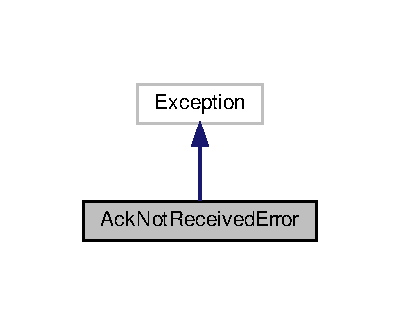
\includegraphics[width=192pt]{classstm__tools_1_1serialflasher_1_1errors_1_1AckNotReceivedError__inherit__graph}
\end{center}
\end{figure}


Collaboration diagram for Ack\+Not\+Received\+Error\+:
\nopagebreak
\begin{figure}[H]
\begin{center}
\leavevmode
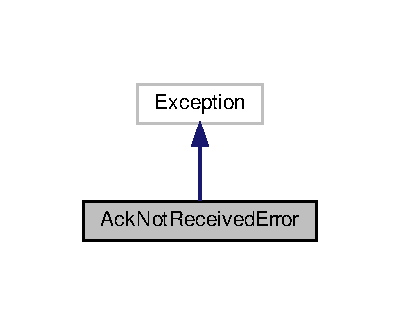
\includegraphics[width=192pt]{classstm__tools_1_1serialflasher_1_1errors_1_1AckNotReceivedError__coll__graph}
\end{center}
\end{figure}


\subsection{Detailed Description}
\begin{DoxyVerb}An expected ack byte was not received\end{DoxyVerb}
 

The documentation for this class was generated from the following file\+:\begin{DoxyCompactItemize}
\item 
/home/rich/\+Development/\+Py\+Dev/\+S\+T\+M32\+Tools/\+S\+T\+M32\+F1\+\_\+\+Serial\+\_\+\+Flasher/stm\+\_\+tools/serialflasher/\hyperlink{errors_8py}{errors.\+py}\end{DoxyCompactItemize}

\hypertarget{classstm__tools_1_1serialflasher_1_1errors_1_1CommandFailedError}{}\section{Command\+Failed\+Error Class Reference}
\label{classstm__tools_1_1serialflasher_1_1errors_1_1CommandFailedError}\index{Command\+Failed\+Error@{Command\+Failed\+Error}}


Inheritance diagram for Command\+Failed\+Error\+:
\nopagebreak
\begin{figure}[H]
\begin{center}
\leavevmode
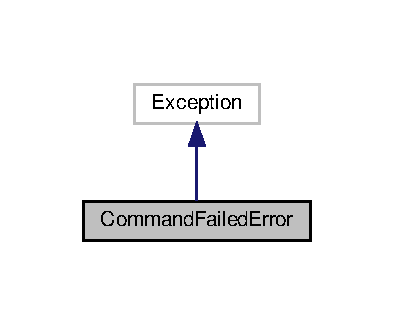
\includegraphics[width=189pt]{classstm__tools_1_1serialflasher_1_1errors_1_1CommandFailedError__inherit__graph}
\end{center}
\end{figure}


Collaboration diagram for Command\+Failed\+Error\+:
\nopagebreak
\begin{figure}[H]
\begin{center}
\leavevmode
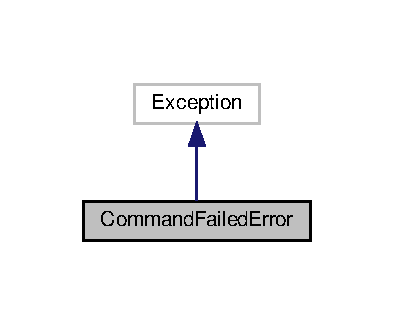
\includegraphics[width=189pt]{classstm__tools_1_1serialflasher_1_1errors_1_1CommandFailedError__coll__graph}
\end{center}
\end{figure}


\subsection{Detailed Description}
\begin{DoxyVerb}The command failed in some way\end{DoxyVerb}
 

The documentation for this class was generated from the following file\+:\begin{DoxyCompactItemize}
\item 
/home/rich/\+Development/\+Py\+Dev/\+S\+T\+M32\+Tools/\+S\+T\+M32\+F1\+\_\+\+Serial\+\_\+\+Flasher/stm\+\_\+tools/serialflasher/\hyperlink{errors_8py}{errors.\+py}\end{DoxyCompactItemize}

\hypertarget{classstm__tools_1_1serialflasher_1_1devices_1_1DeviceDensity}{}\section{Device\+Density Class Reference}
\label{classstm__tools_1_1serialflasher_1_1devices_1_1DeviceDensity}\index{Device\+Density@{Device\+Density}}


Inheritance diagram for Device\+Density\+:
\nopagebreak
\begin{figure}[H]
\begin{center}
\leavevmode
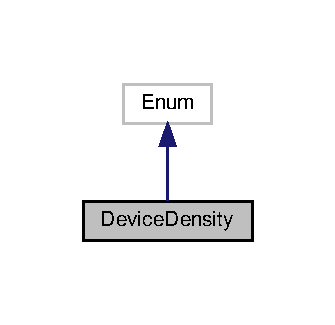
\includegraphics[width=161pt]{classstm__tools_1_1serialflasher_1_1devices_1_1DeviceDensity__inherit__graph}
\end{center}
\end{figure}


Collaboration diagram for Device\+Density\+:
\nopagebreak
\begin{figure}[H]
\begin{center}
\leavevmode
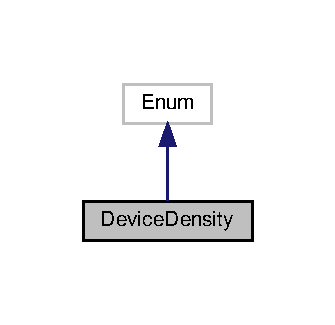
\includegraphics[width=161pt]{classstm__tools_1_1serialflasher_1_1devices_1_1DeviceDensity__coll__graph}
\end{center}
\end{figure}
\subsection*{Static Public Attributes}
\begin{DoxyCompactItemize}
\item 
int \hyperlink{classstm__tools_1_1serialflasher_1_1devices_1_1DeviceDensity_aa366990eb432a5857261b6695d5103e1}{D\+E\+V\+I\+C\+E\+\_\+\+T\+Y\+P\+E\+\_\+\+U\+N\+K\+N\+O\+WN} = 0
\item 
int \hyperlink{classstm__tools_1_1serialflasher_1_1devices_1_1DeviceDensity_a987fd1fab631cf6767c526467d03b809}{D\+E\+V\+I\+C\+E\+\_\+\+T\+Y\+P\+E\+\_\+\+L\+O\+W\+\_\+\+D\+E\+N\+S\+I\+TY} = 1
\item 
int \hyperlink{classstm__tools_1_1serialflasher_1_1devices_1_1DeviceDensity_a111774c04b9d3490c052abb4628efe95}{D\+E\+V\+I\+C\+E\+\_\+\+T\+Y\+P\+E\+\_\+\+M\+E\+D\+I\+U\+M\+\_\+\+D\+E\+N\+S\+I\+TY} = 2
\item 
int \hyperlink{classstm__tools_1_1serialflasher_1_1devices_1_1DeviceDensity_adf7ca92546276150a967a821fa53fc5b}{D\+E\+V\+I\+C\+E\+\_\+\+T\+Y\+P\+E\+\_\+\+H\+I\+G\+H\+\_\+\+D\+E\+N\+S\+I\+TY} = 3
\item 
int \hyperlink{classstm__tools_1_1serialflasher_1_1devices_1_1DeviceDensity_afdb0be7b9130a97eeedb21b56eb8b1f7}{D\+E\+V\+I\+C\+E\+\_\+\+T\+Y\+P\+E\+\_\+\+X\+L\+\_\+\+D\+E\+N\+S\+I\+TY} = 4
\end{DoxyCompactItemize}


\subsection{Member Data Documentation}
\mbox{\Hypertarget{classstm__tools_1_1serialflasher_1_1devices_1_1DeviceDensity_adf7ca92546276150a967a821fa53fc5b}\label{classstm__tools_1_1serialflasher_1_1devices_1_1DeviceDensity_adf7ca92546276150a967a821fa53fc5b}} 
\index{stm\+\_\+tools\+::serialflasher\+::devices\+::\+Device\+Density@{stm\+\_\+tools\+::serialflasher\+::devices\+::\+Device\+Density}!D\+E\+V\+I\+C\+E\+\_\+\+T\+Y\+P\+E\+\_\+\+H\+I\+G\+H\+\_\+\+D\+E\+N\+S\+I\+TY@{D\+E\+V\+I\+C\+E\+\_\+\+T\+Y\+P\+E\+\_\+\+H\+I\+G\+H\+\_\+\+D\+E\+N\+S\+I\+TY}}
\index{D\+E\+V\+I\+C\+E\+\_\+\+T\+Y\+P\+E\+\_\+\+H\+I\+G\+H\+\_\+\+D\+E\+N\+S\+I\+TY@{D\+E\+V\+I\+C\+E\+\_\+\+T\+Y\+P\+E\+\_\+\+H\+I\+G\+H\+\_\+\+D\+E\+N\+S\+I\+TY}!stm\+\_\+tools\+::serialflasher\+::devices\+::\+Device\+Density@{stm\+\_\+tools\+::serialflasher\+::devices\+::\+Device\+Density}}
\subsubsection{\texorpdfstring{D\+E\+V\+I\+C\+E\+\_\+\+T\+Y\+P\+E\+\_\+\+H\+I\+G\+H\+\_\+\+D\+E\+N\+S\+I\+TY}{DEVICE\_TYPE\_HIGH\_DENSITY}}
{\footnotesize\ttfamily int D\+E\+V\+I\+C\+E\+\_\+\+T\+Y\+P\+E\+\_\+\+H\+I\+G\+H\+\_\+\+D\+E\+N\+S\+I\+TY = 3\hspace{0.3cm}{\ttfamily [static]}}

\mbox{\Hypertarget{classstm__tools_1_1serialflasher_1_1devices_1_1DeviceDensity_a987fd1fab631cf6767c526467d03b809}\label{classstm__tools_1_1serialflasher_1_1devices_1_1DeviceDensity_a987fd1fab631cf6767c526467d03b809}} 
\index{stm\+\_\+tools\+::serialflasher\+::devices\+::\+Device\+Density@{stm\+\_\+tools\+::serialflasher\+::devices\+::\+Device\+Density}!D\+E\+V\+I\+C\+E\+\_\+\+T\+Y\+P\+E\+\_\+\+L\+O\+W\+\_\+\+D\+E\+N\+S\+I\+TY@{D\+E\+V\+I\+C\+E\+\_\+\+T\+Y\+P\+E\+\_\+\+L\+O\+W\+\_\+\+D\+E\+N\+S\+I\+TY}}
\index{D\+E\+V\+I\+C\+E\+\_\+\+T\+Y\+P\+E\+\_\+\+L\+O\+W\+\_\+\+D\+E\+N\+S\+I\+TY@{D\+E\+V\+I\+C\+E\+\_\+\+T\+Y\+P\+E\+\_\+\+L\+O\+W\+\_\+\+D\+E\+N\+S\+I\+TY}!stm\+\_\+tools\+::serialflasher\+::devices\+::\+Device\+Density@{stm\+\_\+tools\+::serialflasher\+::devices\+::\+Device\+Density}}
\subsubsection{\texorpdfstring{D\+E\+V\+I\+C\+E\+\_\+\+T\+Y\+P\+E\+\_\+\+L\+O\+W\+\_\+\+D\+E\+N\+S\+I\+TY}{DEVICE\_TYPE\_LOW\_DENSITY}}
{\footnotesize\ttfamily int D\+E\+V\+I\+C\+E\+\_\+\+T\+Y\+P\+E\+\_\+\+L\+O\+W\+\_\+\+D\+E\+N\+S\+I\+TY = 1\hspace{0.3cm}{\ttfamily [static]}}

\mbox{\Hypertarget{classstm__tools_1_1serialflasher_1_1devices_1_1DeviceDensity_a111774c04b9d3490c052abb4628efe95}\label{classstm__tools_1_1serialflasher_1_1devices_1_1DeviceDensity_a111774c04b9d3490c052abb4628efe95}} 
\index{stm\+\_\+tools\+::serialflasher\+::devices\+::\+Device\+Density@{stm\+\_\+tools\+::serialflasher\+::devices\+::\+Device\+Density}!D\+E\+V\+I\+C\+E\+\_\+\+T\+Y\+P\+E\+\_\+\+M\+E\+D\+I\+U\+M\+\_\+\+D\+E\+N\+S\+I\+TY@{D\+E\+V\+I\+C\+E\+\_\+\+T\+Y\+P\+E\+\_\+\+M\+E\+D\+I\+U\+M\+\_\+\+D\+E\+N\+S\+I\+TY}}
\index{D\+E\+V\+I\+C\+E\+\_\+\+T\+Y\+P\+E\+\_\+\+M\+E\+D\+I\+U\+M\+\_\+\+D\+E\+N\+S\+I\+TY@{D\+E\+V\+I\+C\+E\+\_\+\+T\+Y\+P\+E\+\_\+\+M\+E\+D\+I\+U\+M\+\_\+\+D\+E\+N\+S\+I\+TY}!stm\+\_\+tools\+::serialflasher\+::devices\+::\+Device\+Density@{stm\+\_\+tools\+::serialflasher\+::devices\+::\+Device\+Density}}
\subsubsection{\texorpdfstring{D\+E\+V\+I\+C\+E\+\_\+\+T\+Y\+P\+E\+\_\+\+M\+E\+D\+I\+U\+M\+\_\+\+D\+E\+N\+S\+I\+TY}{DEVICE\_TYPE\_MEDIUM\_DENSITY}}
{\footnotesize\ttfamily int D\+E\+V\+I\+C\+E\+\_\+\+T\+Y\+P\+E\+\_\+\+M\+E\+D\+I\+U\+M\+\_\+\+D\+E\+N\+S\+I\+TY = 2\hspace{0.3cm}{\ttfamily [static]}}

\mbox{\Hypertarget{classstm__tools_1_1serialflasher_1_1devices_1_1DeviceDensity_aa366990eb432a5857261b6695d5103e1}\label{classstm__tools_1_1serialflasher_1_1devices_1_1DeviceDensity_aa366990eb432a5857261b6695d5103e1}} 
\index{stm\+\_\+tools\+::serialflasher\+::devices\+::\+Device\+Density@{stm\+\_\+tools\+::serialflasher\+::devices\+::\+Device\+Density}!D\+E\+V\+I\+C\+E\+\_\+\+T\+Y\+P\+E\+\_\+\+U\+N\+K\+N\+O\+WN@{D\+E\+V\+I\+C\+E\+\_\+\+T\+Y\+P\+E\+\_\+\+U\+N\+K\+N\+O\+WN}}
\index{D\+E\+V\+I\+C\+E\+\_\+\+T\+Y\+P\+E\+\_\+\+U\+N\+K\+N\+O\+WN@{D\+E\+V\+I\+C\+E\+\_\+\+T\+Y\+P\+E\+\_\+\+U\+N\+K\+N\+O\+WN}!stm\+\_\+tools\+::serialflasher\+::devices\+::\+Device\+Density@{stm\+\_\+tools\+::serialflasher\+::devices\+::\+Device\+Density}}
\subsubsection{\texorpdfstring{D\+E\+V\+I\+C\+E\+\_\+\+T\+Y\+P\+E\+\_\+\+U\+N\+K\+N\+O\+WN}{DEVICE\_TYPE\_UNKNOWN}}
{\footnotesize\ttfamily int D\+E\+V\+I\+C\+E\+\_\+\+T\+Y\+P\+E\+\_\+\+U\+N\+K\+N\+O\+WN = 0\hspace{0.3cm}{\ttfamily [static]}}

\mbox{\Hypertarget{classstm__tools_1_1serialflasher_1_1devices_1_1DeviceDensity_afdb0be7b9130a97eeedb21b56eb8b1f7}\label{classstm__tools_1_1serialflasher_1_1devices_1_1DeviceDensity_afdb0be7b9130a97eeedb21b56eb8b1f7}} 
\index{stm\+\_\+tools\+::serialflasher\+::devices\+::\+Device\+Density@{stm\+\_\+tools\+::serialflasher\+::devices\+::\+Device\+Density}!D\+E\+V\+I\+C\+E\+\_\+\+T\+Y\+P\+E\+\_\+\+X\+L\+\_\+\+D\+E\+N\+S\+I\+TY@{D\+E\+V\+I\+C\+E\+\_\+\+T\+Y\+P\+E\+\_\+\+X\+L\+\_\+\+D\+E\+N\+S\+I\+TY}}
\index{D\+E\+V\+I\+C\+E\+\_\+\+T\+Y\+P\+E\+\_\+\+X\+L\+\_\+\+D\+E\+N\+S\+I\+TY@{D\+E\+V\+I\+C\+E\+\_\+\+T\+Y\+P\+E\+\_\+\+X\+L\+\_\+\+D\+E\+N\+S\+I\+TY}!stm\+\_\+tools\+::serialflasher\+::devices\+::\+Device\+Density@{stm\+\_\+tools\+::serialflasher\+::devices\+::\+Device\+Density}}
\subsubsection{\texorpdfstring{D\+E\+V\+I\+C\+E\+\_\+\+T\+Y\+P\+E\+\_\+\+X\+L\+\_\+\+D\+E\+N\+S\+I\+TY}{DEVICE\_TYPE\_XL\_DENSITY}}
{\footnotesize\ttfamily int D\+E\+V\+I\+C\+E\+\_\+\+T\+Y\+P\+E\+\_\+\+X\+L\+\_\+\+D\+E\+N\+S\+I\+TY = 4\hspace{0.3cm}{\ttfamily [static]}}



The documentation for this class was generated from the following file\+:\begin{DoxyCompactItemize}
\item 
/home/rich/\+Development/\+Py\+Dev/\+S\+T\+M32\+Tools/\+S\+T\+M32\+F1\+\_\+\+Serial\+\_\+\+Flasher/stm\+\_\+tools/serialflasher/\hyperlink{devices_8py}{devices.\+py}\end{DoxyCompactItemize}

\hypertarget{classstm__tools_1_1serialflasher_1_1errors_1_1DeviceNotConnectedError}{}\section{Device\+Not\+Connected\+Error Class Reference}
\label{classstm__tools_1_1serialflasher_1_1errors_1_1DeviceNotConnectedError}\index{Device\+Not\+Connected\+Error@{Device\+Not\+Connected\+Error}}


Inheritance diagram for Device\+Not\+Connected\+Error\+:
\nopagebreak
\begin{figure}[H]
\begin{center}
\leavevmode
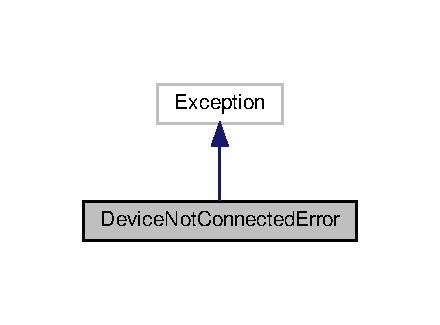
\includegraphics[width=211pt]{classstm__tools_1_1serialflasher_1_1errors_1_1DeviceNotConnectedError__inherit__graph}
\end{center}
\end{figure}


Collaboration diagram for Device\+Not\+Connected\+Error\+:
\nopagebreak
\begin{figure}[H]
\begin{center}
\leavevmode
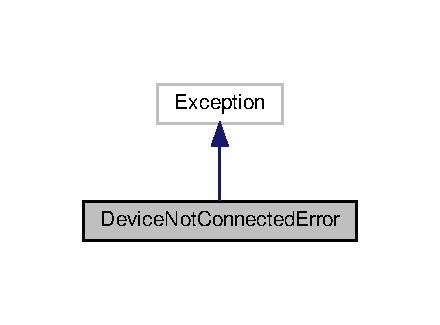
\includegraphics[width=211pt]{classstm__tools_1_1serialflasher_1_1errors_1_1DeviceNotConnectedError__coll__graph}
\end{center}
\end{figure}


\subsection{Detailed Description}
\begin{DoxyVerb}The device is not connected\end{DoxyVerb}
 

The documentation for this class was generated from the following file\+:\begin{DoxyCompactItemize}
\item 
/home/rich/\+Development/\+Py\+Dev/\+S\+T\+M32\+Tools/\+S\+T\+M32\+F1\+\_\+\+Serial\+\_\+\+Flasher/stm\+\_\+tools/serialflasher/\hyperlink{errors_8py}{errors.\+py}\end{DoxyCompactItemize}

\hypertarget{classstm__tools_1_1serialflasher_1_1errors_1_1DeviceNotSupportedError}{}\section{Device\+Not\+Supported\+Error Class Reference}
\label{classstm__tools_1_1serialflasher_1_1errors_1_1DeviceNotSupportedError}\index{Device\+Not\+Supported\+Error@{Device\+Not\+Supported\+Error}}


Inheritance diagram for Device\+Not\+Supported\+Error\+:
\nopagebreak
\begin{figure}[H]
\begin{center}
\leavevmode
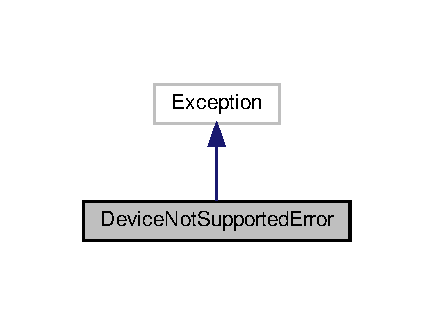
\includegraphics[width=208pt]{classstm__tools_1_1serialflasher_1_1errors_1_1DeviceNotSupportedError__inherit__graph}
\end{center}
\end{figure}


Collaboration diagram for Device\+Not\+Supported\+Error\+:
\nopagebreak
\begin{figure}[H]
\begin{center}
\leavevmode
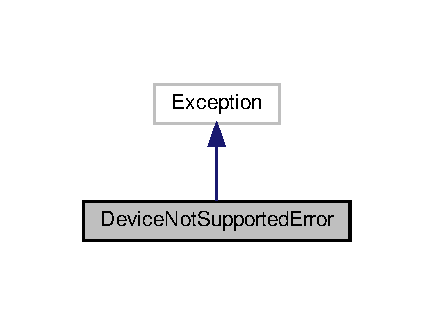
\includegraphics[width=208pt]{classstm__tools_1_1serialflasher_1_1errors_1_1DeviceNotSupportedError__coll__graph}
\end{center}
\end{figure}


\subsection{Detailed Description}
\begin{DoxyVerb}The device is not currently supported\end{DoxyVerb}
 

The documentation for this class was generated from the following file\+:\begin{DoxyCompactItemize}
\item 
/home/rich/\+Development/\+Py\+Dev/\+S\+T\+M32\+Tools/\+S\+T\+M32\+F1\+\_\+\+Serial\+\_\+\+Flasher/stm\+\_\+tools/serialflasher/\hyperlink{errors_8py}{errors.\+py}\end{DoxyCompactItemize}

\hypertarget{classstm__tools_1_1serialflasher_1_1devices_1_1DeviceType}{}\section{Device\+Type Class Reference}
\label{classstm__tools_1_1serialflasher_1_1devices_1_1DeviceType}\index{Device\+Type@{Device\+Type}}
\subsection*{Public Member Functions}
\begin{DoxyCompactItemize}
\item 
def \hyperlink{classstm__tools_1_1serialflasher_1_1devices_1_1DeviceType_ac775ee34451fdfa742b318538164070e}{\+\_\+\+\_\+init\+\_\+\+\_\+}
\item 
def \hyperlink{classstm__tools_1_1serialflasher_1_1devices_1_1DeviceType_af80ad02979239c2550bd7e104e033566}{update\+Option\+Bytes}
\item 
def \hyperlink{classstm__tools_1_1serialflasher_1_1devices_1_1DeviceType_ae57fa7cefa4fcfdef06179d37b0a0a43}{get\+Flash\+Page\+Address}
\end{DoxyCompactItemize}
\subsection*{Public Attributes}
\begin{DoxyCompactItemize}
\item 
\hyperlink{classstm__tools_1_1serialflasher_1_1devices_1_1DeviceType_ac47ca0713353d3fc9435a4f208f6b9a3}{pid}
\item 
\hyperlink{classstm__tools_1_1serialflasher_1_1devices_1_1DeviceType_af9435dc9b903cfa272f9b7caa56c7395}{bootloader\+Version}
\item 
\hyperlink{classstm__tools_1_1serialflasher_1_1devices_1_1DeviceType_a6c37743f24bd50c6555534138bb06609}{bootloader\+\_\+ram}
\item 
\hyperlink{classstm__tools_1_1serialflasher_1_1devices_1_1DeviceType_a8ee7951d8a8b884cd0e3e96ff0e044c9}{system\+\_\+memory}
\item 
\hyperlink{classstm__tools_1_1serialflasher_1_1devices_1_1DeviceType_ab74e6bf80237ddc4109968cedc58c151}{name}
\item 
\hyperlink{classstm__tools_1_1serialflasher_1_1devices_1_1DeviceType_a734379e382de4feb0dce07cb1061ef48}{ram}
\item 
\hyperlink{classstm__tools_1_1serialflasher_1_1devices_1_1DeviceType_a2dad30d94d39cd71e17e3dd0c0d0a56f}{flash\+\_\+page\+\_\+size}
\item 
\hyperlink{classstm__tools_1_1serialflasher_1_1devices_1_1DeviceType_a9540d15c338a785998389ac085d63d60}{flash\+\_\+page\+\_\+num}
\item 
\hyperlink{classstm__tools_1_1serialflasher_1_1devices_1_1DeviceType_ae9e107caabf7796d774e3b9dc66242f6}{flash\+\_\+info\+\_\+blk\+\_\+size}
\item 
\hyperlink{classstm__tools_1_1serialflasher_1_1devices_1_1DeviceType_adead9432d676c0ea71798ca6d28f0dc5}{flash\+\_\+memory}
\item 
\hyperlink{classstm__tools_1_1serialflasher_1_1devices_1_1DeviceType_a7ee6d57cdb63ffd25b774bc45ad88bdd}{flash\+\_\+pages}
\item 
\hyperlink{classstm__tools_1_1serialflasher_1_1devices_1_1DeviceType_ae0dcda22a9424b46b3b203906bff637d}{flash\+\_\+option\+\_\+bytes}
\item 
\hyperlink{classstm__tools_1_1serialflasher_1_1devices_1_1DeviceType_ad14913aeb6f779e1f7d36afffd23d781}{opt\+\_\+bytes}
\begin{DoxyCompactList}\small\item\em fill this in on demand \end{DoxyCompactList}\end{DoxyCompactItemize}
\subsection*{Static Public Attributes}
\begin{DoxyCompactItemize}
\item 
\hyperlink{classstm__tools_1_1serialflasher_1_1devices_1_1DeviceType_a61569f2965b7a369eb10b6d75d410d11}{int}
\end{DoxyCompactItemize}


\subsection{Constructor \& Destructor Documentation}
\mbox{\Hypertarget{classstm__tools_1_1serialflasher_1_1devices_1_1DeviceType_ac775ee34451fdfa742b318538164070e}\label{classstm__tools_1_1serialflasher_1_1devices_1_1DeviceType_ac775ee34451fdfa742b318538164070e}} 
\index{stm\+\_\+tools\+::serialflasher\+::devices\+::\+Device\+Type@{stm\+\_\+tools\+::serialflasher\+::devices\+::\+Device\+Type}!\+\_\+\+\_\+init\+\_\+\+\_\+@{\+\_\+\+\_\+init\+\_\+\+\_\+}}
\index{\+\_\+\+\_\+init\+\_\+\+\_\+@{\+\_\+\+\_\+init\+\_\+\+\_\+}!stm\+\_\+tools\+::serialflasher\+::devices\+::\+Device\+Type@{stm\+\_\+tools\+::serialflasher\+::devices\+::\+Device\+Type}}
\subsubsection{\texorpdfstring{\+\_\+\+\_\+init\+\_\+\+\_\+()}{\_\_init\_\_()}}
{\footnotesize\ttfamily def \+\_\+\+\_\+init\+\_\+\+\_\+ (\begin{DoxyParamCaption}\item[{}]{self,  }\item[{}]{pid }\end{DoxyParamCaption})}



\subsection{Member Function Documentation}
\mbox{\Hypertarget{classstm__tools_1_1serialflasher_1_1devices_1_1DeviceType_ae57fa7cefa4fcfdef06179d37b0a0a43}\label{classstm__tools_1_1serialflasher_1_1devices_1_1DeviceType_ae57fa7cefa4fcfdef06179d37b0a0a43}} 
\index{stm\+\_\+tools\+::serialflasher\+::devices\+::\+Device\+Type@{stm\+\_\+tools\+::serialflasher\+::devices\+::\+Device\+Type}!get\+Flash\+Page\+Address@{get\+Flash\+Page\+Address}}
\index{get\+Flash\+Page\+Address@{get\+Flash\+Page\+Address}!stm\+\_\+tools\+::serialflasher\+::devices\+::\+Device\+Type@{stm\+\_\+tools\+::serialflasher\+::devices\+::\+Device\+Type}}
\subsubsection{\texorpdfstring{get\+Flash\+Page\+Address()}{getFlashPageAddress()}}
{\footnotesize\ttfamily def get\+Flash\+Page\+Address (\begin{DoxyParamCaption}\item[{}]{self,  }\item[{}]{page }\end{DoxyParamCaption})}

\mbox{\Hypertarget{classstm__tools_1_1serialflasher_1_1devices_1_1DeviceType_af80ad02979239c2550bd7e104e033566}\label{classstm__tools_1_1serialflasher_1_1devices_1_1DeviceType_af80ad02979239c2550bd7e104e033566}} 
\index{stm\+\_\+tools\+::serialflasher\+::devices\+::\+Device\+Type@{stm\+\_\+tools\+::serialflasher\+::devices\+::\+Device\+Type}!update\+Option\+Bytes@{update\+Option\+Bytes}}
\index{update\+Option\+Bytes@{update\+Option\+Bytes}!stm\+\_\+tools\+::serialflasher\+::devices\+::\+Device\+Type@{stm\+\_\+tools\+::serialflasher\+::devices\+::\+Device\+Type}}
\subsubsection{\texorpdfstring{update\+Option\+Bytes()}{updateOptionBytes()}}
{\footnotesize\ttfamily def update\+Option\+Bytes (\begin{DoxyParamCaption}\item[{}]{self,  }\item[{}]{data }\end{DoxyParamCaption})}



\subsection{Member Data Documentation}
\mbox{\Hypertarget{classstm__tools_1_1serialflasher_1_1devices_1_1DeviceType_a6c37743f24bd50c6555534138bb06609}\label{classstm__tools_1_1serialflasher_1_1devices_1_1DeviceType_a6c37743f24bd50c6555534138bb06609}} 
\index{stm\+\_\+tools\+::serialflasher\+::devices\+::\+Device\+Type@{stm\+\_\+tools\+::serialflasher\+::devices\+::\+Device\+Type}!bootloader\+\_\+ram@{bootloader\+\_\+ram}}
\index{bootloader\+\_\+ram@{bootloader\+\_\+ram}!stm\+\_\+tools\+::serialflasher\+::devices\+::\+Device\+Type@{stm\+\_\+tools\+::serialflasher\+::devices\+::\+Device\+Type}}
\subsubsection{\texorpdfstring{bootloader\+\_\+ram}{bootloader\_ram}}
{\footnotesize\ttfamily bootloader\+\_\+ram}

\mbox{\Hypertarget{classstm__tools_1_1serialflasher_1_1devices_1_1DeviceType_af9435dc9b903cfa272f9b7caa56c7395}\label{classstm__tools_1_1serialflasher_1_1devices_1_1DeviceType_af9435dc9b903cfa272f9b7caa56c7395}} 
\index{stm\+\_\+tools\+::serialflasher\+::devices\+::\+Device\+Type@{stm\+\_\+tools\+::serialflasher\+::devices\+::\+Device\+Type}!bootloader\+Version@{bootloader\+Version}}
\index{bootloader\+Version@{bootloader\+Version}!stm\+\_\+tools\+::serialflasher\+::devices\+::\+Device\+Type@{stm\+\_\+tools\+::serialflasher\+::devices\+::\+Device\+Type}}
\subsubsection{\texorpdfstring{bootloader\+Version}{bootloaderVersion}}
{\footnotesize\ttfamily bootloader\+Version}

\mbox{\Hypertarget{classstm__tools_1_1serialflasher_1_1devices_1_1DeviceType_ae9e107caabf7796d774e3b9dc66242f6}\label{classstm__tools_1_1serialflasher_1_1devices_1_1DeviceType_ae9e107caabf7796d774e3b9dc66242f6}} 
\index{stm\+\_\+tools\+::serialflasher\+::devices\+::\+Device\+Type@{stm\+\_\+tools\+::serialflasher\+::devices\+::\+Device\+Type}!flash\+\_\+info\+\_\+blk\+\_\+size@{flash\+\_\+info\+\_\+blk\+\_\+size}}
\index{flash\+\_\+info\+\_\+blk\+\_\+size@{flash\+\_\+info\+\_\+blk\+\_\+size}!stm\+\_\+tools\+::serialflasher\+::devices\+::\+Device\+Type@{stm\+\_\+tools\+::serialflasher\+::devices\+::\+Device\+Type}}
\subsubsection{\texorpdfstring{flash\+\_\+info\+\_\+blk\+\_\+size}{flash\_info\_blk\_size}}
{\footnotesize\ttfamily flash\+\_\+info\+\_\+blk\+\_\+size}

\mbox{\Hypertarget{classstm__tools_1_1serialflasher_1_1devices_1_1DeviceType_adead9432d676c0ea71798ca6d28f0dc5}\label{classstm__tools_1_1serialflasher_1_1devices_1_1DeviceType_adead9432d676c0ea71798ca6d28f0dc5}} 
\index{stm\+\_\+tools\+::serialflasher\+::devices\+::\+Device\+Type@{stm\+\_\+tools\+::serialflasher\+::devices\+::\+Device\+Type}!flash\+\_\+memory@{flash\+\_\+memory}}
\index{flash\+\_\+memory@{flash\+\_\+memory}!stm\+\_\+tools\+::serialflasher\+::devices\+::\+Device\+Type@{stm\+\_\+tools\+::serialflasher\+::devices\+::\+Device\+Type}}
\subsubsection{\texorpdfstring{flash\+\_\+memory}{flash\_memory}}
{\footnotesize\ttfamily flash\+\_\+memory}

\mbox{\Hypertarget{classstm__tools_1_1serialflasher_1_1devices_1_1DeviceType_ae0dcda22a9424b46b3b203906bff637d}\label{classstm__tools_1_1serialflasher_1_1devices_1_1DeviceType_ae0dcda22a9424b46b3b203906bff637d}} 
\index{stm\+\_\+tools\+::serialflasher\+::devices\+::\+Device\+Type@{stm\+\_\+tools\+::serialflasher\+::devices\+::\+Device\+Type}!flash\+\_\+option\+\_\+bytes@{flash\+\_\+option\+\_\+bytes}}
\index{flash\+\_\+option\+\_\+bytes@{flash\+\_\+option\+\_\+bytes}!stm\+\_\+tools\+::serialflasher\+::devices\+::\+Device\+Type@{stm\+\_\+tools\+::serialflasher\+::devices\+::\+Device\+Type}}
\subsubsection{\texorpdfstring{flash\+\_\+option\+\_\+bytes}{flash\_option\_bytes}}
{\footnotesize\ttfamily flash\+\_\+option\+\_\+bytes}

\mbox{\Hypertarget{classstm__tools_1_1serialflasher_1_1devices_1_1DeviceType_a9540d15c338a785998389ac085d63d60}\label{classstm__tools_1_1serialflasher_1_1devices_1_1DeviceType_a9540d15c338a785998389ac085d63d60}} 
\index{stm\+\_\+tools\+::serialflasher\+::devices\+::\+Device\+Type@{stm\+\_\+tools\+::serialflasher\+::devices\+::\+Device\+Type}!flash\+\_\+page\+\_\+num@{flash\+\_\+page\+\_\+num}}
\index{flash\+\_\+page\+\_\+num@{flash\+\_\+page\+\_\+num}!stm\+\_\+tools\+::serialflasher\+::devices\+::\+Device\+Type@{stm\+\_\+tools\+::serialflasher\+::devices\+::\+Device\+Type}}
\subsubsection{\texorpdfstring{flash\+\_\+page\+\_\+num}{flash\_page\_num}}
{\footnotesize\ttfamily flash\+\_\+page\+\_\+num}

\mbox{\Hypertarget{classstm__tools_1_1serialflasher_1_1devices_1_1DeviceType_a2dad30d94d39cd71e17e3dd0c0d0a56f}\label{classstm__tools_1_1serialflasher_1_1devices_1_1DeviceType_a2dad30d94d39cd71e17e3dd0c0d0a56f}} 
\index{stm\+\_\+tools\+::serialflasher\+::devices\+::\+Device\+Type@{stm\+\_\+tools\+::serialflasher\+::devices\+::\+Device\+Type}!flash\+\_\+page\+\_\+size@{flash\+\_\+page\+\_\+size}}
\index{flash\+\_\+page\+\_\+size@{flash\+\_\+page\+\_\+size}!stm\+\_\+tools\+::serialflasher\+::devices\+::\+Device\+Type@{stm\+\_\+tools\+::serialflasher\+::devices\+::\+Device\+Type}}
\subsubsection{\texorpdfstring{flash\+\_\+page\+\_\+size}{flash\_page\_size}}
{\footnotesize\ttfamily flash\+\_\+page\+\_\+size}

\mbox{\Hypertarget{classstm__tools_1_1serialflasher_1_1devices_1_1DeviceType_a7ee6d57cdb63ffd25b774bc45ad88bdd}\label{classstm__tools_1_1serialflasher_1_1devices_1_1DeviceType_a7ee6d57cdb63ffd25b774bc45ad88bdd}} 
\index{stm\+\_\+tools\+::serialflasher\+::devices\+::\+Device\+Type@{stm\+\_\+tools\+::serialflasher\+::devices\+::\+Device\+Type}!flash\+\_\+pages@{flash\+\_\+pages}}
\index{flash\+\_\+pages@{flash\+\_\+pages}!stm\+\_\+tools\+::serialflasher\+::devices\+::\+Device\+Type@{stm\+\_\+tools\+::serialflasher\+::devices\+::\+Device\+Type}}
\subsubsection{\texorpdfstring{flash\+\_\+pages}{flash\_pages}}
{\footnotesize\ttfamily flash\+\_\+pages}

\mbox{\Hypertarget{classstm__tools_1_1serialflasher_1_1devices_1_1DeviceType_a61569f2965b7a369eb10b6d75d410d11}\label{classstm__tools_1_1serialflasher_1_1devices_1_1DeviceType_a61569f2965b7a369eb10b6d75d410d11}} 
\index{stm\+\_\+tools\+::serialflasher\+::devices\+::\+Device\+Type@{stm\+\_\+tools\+::serialflasher\+::devices\+::\+Device\+Type}!int@{int}}
\index{int@{int}!stm\+\_\+tools\+::serialflasher\+::devices\+::\+Device\+Type@{stm\+\_\+tools\+::serialflasher\+::devices\+::\+Device\+Type}}
\subsubsection{\texorpdfstring{int}{int}}
{\footnotesize\ttfamily int\hspace{0.3cm}{\ttfamily [static]}}

\mbox{\Hypertarget{classstm__tools_1_1serialflasher_1_1devices_1_1DeviceType_ab74e6bf80237ddc4109968cedc58c151}\label{classstm__tools_1_1serialflasher_1_1devices_1_1DeviceType_ab74e6bf80237ddc4109968cedc58c151}} 
\index{stm\+\_\+tools\+::serialflasher\+::devices\+::\+Device\+Type@{stm\+\_\+tools\+::serialflasher\+::devices\+::\+Device\+Type}!name@{name}}
\index{name@{name}!stm\+\_\+tools\+::serialflasher\+::devices\+::\+Device\+Type@{stm\+\_\+tools\+::serialflasher\+::devices\+::\+Device\+Type}}
\subsubsection{\texorpdfstring{name}{name}}
{\footnotesize\ttfamily name}

\mbox{\Hypertarget{classstm__tools_1_1serialflasher_1_1devices_1_1DeviceType_ad14913aeb6f779e1f7d36afffd23d781}\label{classstm__tools_1_1serialflasher_1_1devices_1_1DeviceType_ad14913aeb6f779e1f7d36afffd23d781}} 
\index{stm\+\_\+tools\+::serialflasher\+::devices\+::\+Device\+Type@{stm\+\_\+tools\+::serialflasher\+::devices\+::\+Device\+Type}!opt\+\_\+bytes@{opt\+\_\+bytes}}
\index{opt\+\_\+bytes@{opt\+\_\+bytes}!stm\+\_\+tools\+::serialflasher\+::devices\+::\+Device\+Type@{stm\+\_\+tools\+::serialflasher\+::devices\+::\+Device\+Type}}
\subsubsection{\texorpdfstring{opt\+\_\+bytes}{opt\_bytes}}
{\footnotesize\ttfamily opt\+\_\+bytes}



fill this in on demand 

\mbox{\Hypertarget{classstm__tools_1_1serialflasher_1_1devices_1_1DeviceType_ac47ca0713353d3fc9435a4f208f6b9a3}\label{classstm__tools_1_1serialflasher_1_1devices_1_1DeviceType_ac47ca0713353d3fc9435a4f208f6b9a3}} 
\index{stm\+\_\+tools\+::serialflasher\+::devices\+::\+Device\+Type@{stm\+\_\+tools\+::serialflasher\+::devices\+::\+Device\+Type}!pid@{pid}}
\index{pid@{pid}!stm\+\_\+tools\+::serialflasher\+::devices\+::\+Device\+Type@{stm\+\_\+tools\+::serialflasher\+::devices\+::\+Device\+Type}}
\subsubsection{\texorpdfstring{pid}{pid}}
{\footnotesize\ttfamily pid}

\mbox{\Hypertarget{classstm__tools_1_1serialflasher_1_1devices_1_1DeviceType_a734379e382de4feb0dce07cb1061ef48}\label{classstm__tools_1_1serialflasher_1_1devices_1_1DeviceType_a734379e382de4feb0dce07cb1061ef48}} 
\index{stm\+\_\+tools\+::serialflasher\+::devices\+::\+Device\+Type@{stm\+\_\+tools\+::serialflasher\+::devices\+::\+Device\+Type}!ram@{ram}}
\index{ram@{ram}!stm\+\_\+tools\+::serialflasher\+::devices\+::\+Device\+Type@{stm\+\_\+tools\+::serialflasher\+::devices\+::\+Device\+Type}}
\subsubsection{\texorpdfstring{ram}{ram}}
{\footnotesize\ttfamily ram}

\mbox{\Hypertarget{classstm__tools_1_1serialflasher_1_1devices_1_1DeviceType_a8ee7951d8a8b884cd0e3e96ff0e044c9}\label{classstm__tools_1_1serialflasher_1_1devices_1_1DeviceType_a8ee7951d8a8b884cd0e3e96ff0e044c9}} 
\index{stm\+\_\+tools\+::serialflasher\+::devices\+::\+Device\+Type@{stm\+\_\+tools\+::serialflasher\+::devices\+::\+Device\+Type}!system\+\_\+memory@{system\+\_\+memory}}
\index{system\+\_\+memory@{system\+\_\+memory}!stm\+\_\+tools\+::serialflasher\+::devices\+::\+Device\+Type@{stm\+\_\+tools\+::serialflasher\+::devices\+::\+Device\+Type}}
\subsubsection{\texorpdfstring{system\+\_\+memory}{system\_memory}}
{\footnotesize\ttfamily system\+\_\+memory}



The documentation for this class was generated from the following file\+:\begin{DoxyCompactItemize}
\item 
/home/rich/\+Development/\+Py\+Dev/\+S\+T\+M32\+Tools/\+S\+T\+M32\+F1\+\_\+\+Serial\+\_\+\+Flasher/stm\+\_\+tools/serialflasher/\hyperlink{devices_8py}{devices.\+py}\end{DoxyCompactItemize}

\hypertarget{classstm__tools_1_1tests_1_1devicetype__test_1_1DeviceTypeTestCase}{}\section{Device\+Type\+Test\+Case Class Reference}
\label{classstm__tools_1_1tests_1_1devicetype__test_1_1DeviceTypeTestCase}\index{Device\+Type\+Test\+Case@{Device\+Type\+Test\+Case}}


Inheritance diagram for Device\+Type\+Test\+Case\+:
\nopagebreak
\begin{figure}[H]
\begin{center}
\leavevmode
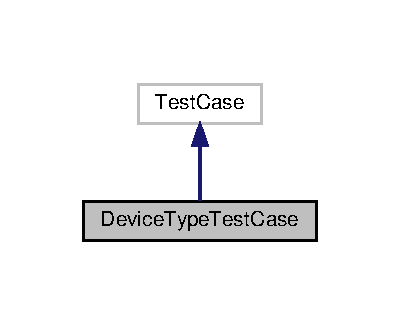
\includegraphics[width=192pt]{classstm__tools_1_1tests_1_1devicetype__test_1_1DeviceTypeTestCase__inherit__graph}
\end{center}
\end{figure}


Collaboration diagram for Device\+Type\+Test\+Case\+:
\nopagebreak
\begin{figure}[H]
\begin{center}
\leavevmode
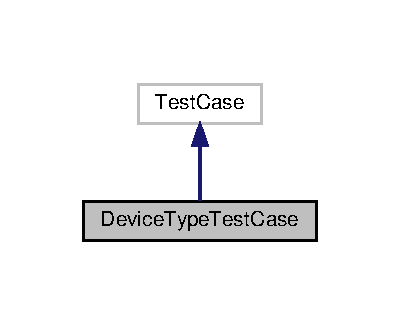
\includegraphics[width=192pt]{classstm__tools_1_1tests_1_1devicetype__test_1_1DeviceTypeTestCase__coll__graph}
\end{center}
\end{figure}
\subsection*{Public Member Functions}
\begin{DoxyCompactItemize}
\item 
def \hyperlink{classstm__tools_1_1tests_1_1devicetype__test_1_1DeviceTypeTestCase_a44235804fcdd3742539311a5b227cd65}{test\+Init\+Device\+Valid\+Id} (self)
\item 
def \hyperlink{classstm__tools_1_1tests_1_1devicetype__test_1_1DeviceTypeTestCase_a34ba45e3d34c504190cfdda52c974106}{test\+Init\+Device\+Invalid\+Id} (self)
\item 
def \hyperlink{classstm__tools_1_1tests_1_1devicetype__test_1_1DeviceTypeTestCase_a4fb9c46c063bdb33ee776b5bfaed520c}{test\+Device\+Bootloader\+Type} (self)
\item 
def \hyperlink{classstm__tools_1_1tests_1_1devicetype__test_1_1DeviceTypeTestCase_aeea2f380b7d7106f7828562b2582c2c1}{test\+Device\+Bootloader\+Region\+Size} (self)
\item 
def \hyperlink{classstm__tools_1_1tests_1_1devicetype__test_1_1DeviceTypeTestCase_a02d45ddc1e867ec1642eec0a5803e540}{test\+Device\+Flash\+Memory\+Size} (self)
\item 
def \hyperlink{classstm__tools_1_1tests_1_1devicetype__test_1_1DeviceTypeTestCase_aac994f12a19d50c45d0e86e833c62f10}{test\+Option\+Bytes\+Update} (self)
\end{DoxyCompactItemize}


\subsection{Member Function Documentation}
\mbox{\Hypertarget{classstm__tools_1_1tests_1_1devicetype__test_1_1DeviceTypeTestCase_aeea2f380b7d7106f7828562b2582c2c1}\label{classstm__tools_1_1tests_1_1devicetype__test_1_1DeviceTypeTestCase_aeea2f380b7d7106f7828562b2582c2c1}} 
\index{stm\+\_\+tools\+::tests\+::devicetype\+\_\+test\+::\+Device\+Type\+Test\+Case@{stm\+\_\+tools\+::tests\+::devicetype\+\_\+test\+::\+Device\+Type\+Test\+Case}!test\+Device\+Bootloader\+Region\+Size@{test\+Device\+Bootloader\+Region\+Size}}
\index{test\+Device\+Bootloader\+Region\+Size@{test\+Device\+Bootloader\+Region\+Size}!stm\+\_\+tools\+::tests\+::devicetype\+\_\+test\+::\+Device\+Type\+Test\+Case@{stm\+\_\+tools\+::tests\+::devicetype\+\_\+test\+::\+Device\+Type\+Test\+Case}}
\subsubsection{\texorpdfstring{test\+Device\+Bootloader\+Region\+Size()}{testDeviceBootloaderRegionSize()}}
{\footnotesize\ttfamily def test\+Device\+Bootloader\+Region\+Size (\begin{DoxyParamCaption}\item[{}]{self }\end{DoxyParamCaption})}

\mbox{\Hypertarget{classstm__tools_1_1tests_1_1devicetype__test_1_1DeviceTypeTestCase_a4fb9c46c063bdb33ee776b5bfaed520c}\label{classstm__tools_1_1tests_1_1devicetype__test_1_1DeviceTypeTestCase_a4fb9c46c063bdb33ee776b5bfaed520c}} 
\index{stm\+\_\+tools\+::tests\+::devicetype\+\_\+test\+::\+Device\+Type\+Test\+Case@{stm\+\_\+tools\+::tests\+::devicetype\+\_\+test\+::\+Device\+Type\+Test\+Case}!test\+Device\+Bootloader\+Type@{test\+Device\+Bootloader\+Type}}
\index{test\+Device\+Bootloader\+Type@{test\+Device\+Bootloader\+Type}!stm\+\_\+tools\+::tests\+::devicetype\+\_\+test\+::\+Device\+Type\+Test\+Case@{stm\+\_\+tools\+::tests\+::devicetype\+\_\+test\+::\+Device\+Type\+Test\+Case}}
\subsubsection{\texorpdfstring{test\+Device\+Bootloader\+Type()}{testDeviceBootloaderType()}}
{\footnotesize\ttfamily def test\+Device\+Bootloader\+Type (\begin{DoxyParamCaption}\item[{}]{self }\end{DoxyParamCaption})}

\mbox{\Hypertarget{classstm__tools_1_1tests_1_1devicetype__test_1_1DeviceTypeTestCase_a02d45ddc1e867ec1642eec0a5803e540}\label{classstm__tools_1_1tests_1_1devicetype__test_1_1DeviceTypeTestCase_a02d45ddc1e867ec1642eec0a5803e540}} 
\index{stm\+\_\+tools\+::tests\+::devicetype\+\_\+test\+::\+Device\+Type\+Test\+Case@{stm\+\_\+tools\+::tests\+::devicetype\+\_\+test\+::\+Device\+Type\+Test\+Case}!test\+Device\+Flash\+Memory\+Size@{test\+Device\+Flash\+Memory\+Size}}
\index{test\+Device\+Flash\+Memory\+Size@{test\+Device\+Flash\+Memory\+Size}!stm\+\_\+tools\+::tests\+::devicetype\+\_\+test\+::\+Device\+Type\+Test\+Case@{stm\+\_\+tools\+::tests\+::devicetype\+\_\+test\+::\+Device\+Type\+Test\+Case}}
\subsubsection{\texorpdfstring{test\+Device\+Flash\+Memory\+Size()}{testDeviceFlashMemorySize()}}
{\footnotesize\ttfamily def test\+Device\+Flash\+Memory\+Size (\begin{DoxyParamCaption}\item[{}]{self }\end{DoxyParamCaption})}

\mbox{\Hypertarget{classstm__tools_1_1tests_1_1devicetype__test_1_1DeviceTypeTestCase_a34ba45e3d34c504190cfdda52c974106}\label{classstm__tools_1_1tests_1_1devicetype__test_1_1DeviceTypeTestCase_a34ba45e3d34c504190cfdda52c974106}} 
\index{stm\+\_\+tools\+::tests\+::devicetype\+\_\+test\+::\+Device\+Type\+Test\+Case@{stm\+\_\+tools\+::tests\+::devicetype\+\_\+test\+::\+Device\+Type\+Test\+Case}!test\+Init\+Device\+Invalid\+Id@{test\+Init\+Device\+Invalid\+Id}}
\index{test\+Init\+Device\+Invalid\+Id@{test\+Init\+Device\+Invalid\+Id}!stm\+\_\+tools\+::tests\+::devicetype\+\_\+test\+::\+Device\+Type\+Test\+Case@{stm\+\_\+tools\+::tests\+::devicetype\+\_\+test\+::\+Device\+Type\+Test\+Case}}
\subsubsection{\texorpdfstring{test\+Init\+Device\+Invalid\+Id()}{testInitDeviceInvalidId()}}
{\footnotesize\ttfamily def test\+Init\+Device\+Invalid\+Id (\begin{DoxyParamCaption}\item[{}]{self }\end{DoxyParamCaption})}

\mbox{\Hypertarget{classstm__tools_1_1tests_1_1devicetype__test_1_1DeviceTypeTestCase_a44235804fcdd3742539311a5b227cd65}\label{classstm__tools_1_1tests_1_1devicetype__test_1_1DeviceTypeTestCase_a44235804fcdd3742539311a5b227cd65}} 
\index{stm\+\_\+tools\+::tests\+::devicetype\+\_\+test\+::\+Device\+Type\+Test\+Case@{stm\+\_\+tools\+::tests\+::devicetype\+\_\+test\+::\+Device\+Type\+Test\+Case}!test\+Init\+Device\+Valid\+Id@{test\+Init\+Device\+Valid\+Id}}
\index{test\+Init\+Device\+Valid\+Id@{test\+Init\+Device\+Valid\+Id}!stm\+\_\+tools\+::tests\+::devicetype\+\_\+test\+::\+Device\+Type\+Test\+Case@{stm\+\_\+tools\+::tests\+::devicetype\+\_\+test\+::\+Device\+Type\+Test\+Case}}
\subsubsection{\texorpdfstring{test\+Init\+Device\+Valid\+Id()}{testInitDeviceValidId()}}
{\footnotesize\ttfamily def test\+Init\+Device\+Valid\+Id (\begin{DoxyParamCaption}\item[{}]{self }\end{DoxyParamCaption})}

\mbox{\Hypertarget{classstm__tools_1_1tests_1_1devicetype__test_1_1DeviceTypeTestCase_aac994f12a19d50c45d0e86e833c62f10}\label{classstm__tools_1_1tests_1_1devicetype__test_1_1DeviceTypeTestCase_aac994f12a19d50c45d0e86e833c62f10}} 
\index{stm\+\_\+tools\+::tests\+::devicetype\+\_\+test\+::\+Device\+Type\+Test\+Case@{stm\+\_\+tools\+::tests\+::devicetype\+\_\+test\+::\+Device\+Type\+Test\+Case}!test\+Option\+Bytes\+Update@{test\+Option\+Bytes\+Update}}
\index{test\+Option\+Bytes\+Update@{test\+Option\+Bytes\+Update}!stm\+\_\+tools\+::tests\+::devicetype\+\_\+test\+::\+Device\+Type\+Test\+Case@{stm\+\_\+tools\+::tests\+::devicetype\+\_\+test\+::\+Device\+Type\+Test\+Case}}
\subsubsection{\texorpdfstring{test\+Option\+Bytes\+Update()}{testOptionBytesUpdate()}}
{\footnotesize\ttfamily def test\+Option\+Bytes\+Update (\begin{DoxyParamCaption}\item[{}]{self }\end{DoxyParamCaption})}



The documentation for this class was generated from the following file\+:\begin{DoxyCompactItemize}
\item 
/home/rich/\+Development/\+Py\+Dev/\+S\+T\+M32\+Tools/\+S\+T\+M32\+F1\+\_\+\+Serial\+\_\+\+Flasher/stm\+\_\+tools/tests/\hyperlink{devicetype__test_8py}{devicetype\+\_\+test.\+py}\end{DoxyCompactItemize}

\hypertarget{classstm__tools_1_1serialflasher_1_1errors_1_1InformationNotRetrieved}{}\section{Information\+Not\+Retrieved Class Reference}
\label{classstm__tools_1_1serialflasher_1_1errors_1_1InformationNotRetrieved}\index{Information\+Not\+Retrieved@{Information\+Not\+Retrieved}}


Inheritance diagram for Information\+Not\+Retrieved\+:
\nopagebreak
\begin{figure}[H]
\begin{center}
\leavevmode
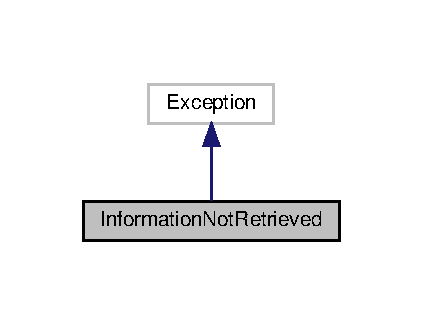
\includegraphics[width=203pt]{classstm__tools_1_1serialflasher_1_1errors_1_1InformationNotRetrieved__inherit__graph}
\end{center}
\end{figure}


Collaboration diagram for Information\+Not\+Retrieved\+:
\nopagebreak
\begin{figure}[H]
\begin{center}
\leavevmode
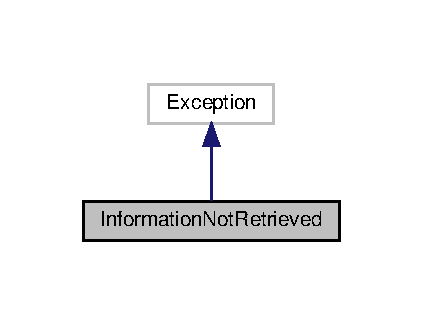
\includegraphics[width=203pt]{classstm__tools_1_1serialflasher_1_1errors_1_1InformationNotRetrieved__coll__graph}
\end{center}
\end{figure}


\subsection{Detailed Description}
\begin{DoxyVerb}information has not been read yet\end{DoxyVerb}
 

The documentation for this class was generated from the following file\+:\begin{DoxyCompactItemize}
\item 
/home/rich/\+Development/\+Py\+Dev/\+S\+T\+M32\+Tools/\+S\+T\+M32\+F1\+\_\+\+Serial\+\_\+\+Flasher/stm\+\_\+tools/serialflasher/\hyperlink{errors_8py}{errors.\+py}\end{DoxyCompactItemize}

\hypertarget{classstm__tools_1_1serialflasher_1_1errors_1_1InvalidAddressError}{}\section{Invalid\+Address\+Error Class Reference}
\label{classstm__tools_1_1serialflasher_1_1errors_1_1InvalidAddressError}\index{Invalid\+Address\+Error@{Invalid\+Address\+Error}}


Inheritance diagram for Invalid\+Address\+Error\+:
\nopagebreak
\begin{figure}[H]
\begin{center}
\leavevmode
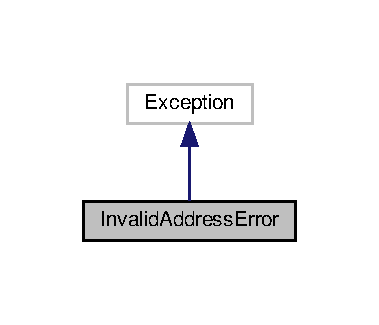
\includegraphics[width=182pt]{classstm__tools_1_1serialflasher_1_1errors_1_1InvalidAddressError__inherit__graph}
\end{center}
\end{figure}


Collaboration diagram for Invalid\+Address\+Error\+:
\nopagebreak
\begin{figure}[H]
\begin{center}
\leavevmode
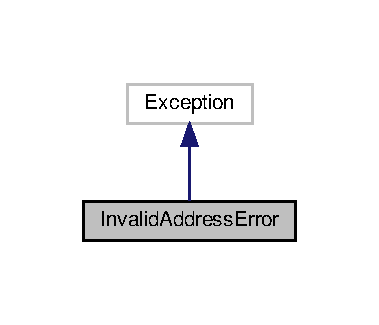
\includegraphics[width=182pt]{classstm__tools_1_1serialflasher_1_1errors_1_1InvalidAddressError__coll__graph}
\end{center}
\end{figure}


\subsection{Detailed Description}
\begin{DoxyVerb}the address is invalid\end{DoxyVerb}
 

The documentation for this class was generated from the following file\+:\begin{DoxyCompactItemize}
\item 
/home/rich/\+Development/\+Py\+Dev/\+S\+T\+M32\+Tools/\+S\+T\+M32\+F1\+\_\+\+Serial\+\_\+\+Flasher/stm\+\_\+tools/serialflasher/\hyperlink{errors_8py}{errors.\+py}\end{DoxyCompactItemize}

\hypertarget{classstm__tools_1_1serialflasher_1_1errors_1_1InvalidEraseLengthError}{}\section{Invalid\+Erase\+Length\+Error Class Reference}
\label{classstm__tools_1_1serialflasher_1_1errors_1_1InvalidEraseLengthError}\index{Invalid\+Erase\+Length\+Error@{Invalid\+Erase\+Length\+Error}}


Inheritance diagram for Invalid\+Erase\+Length\+Error\+:
\nopagebreak
\begin{figure}[H]
\begin{center}
\leavevmode
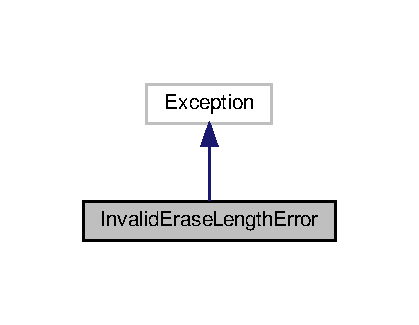
\includegraphics[width=201pt]{classstm__tools_1_1serialflasher_1_1errors_1_1InvalidEraseLengthError__inherit__graph}
\end{center}
\end{figure}


Collaboration diagram for Invalid\+Erase\+Length\+Error\+:
\nopagebreak
\begin{figure}[H]
\begin{center}
\leavevmode
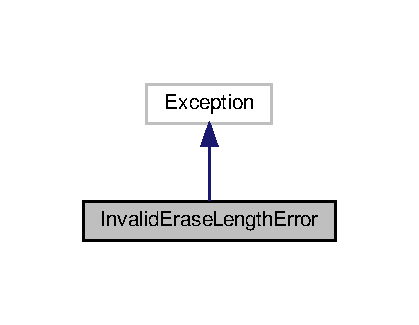
\includegraphics[width=201pt]{classstm__tools_1_1serialflasher_1_1errors_1_1InvalidEraseLengthError__coll__graph}
\end{center}
\end{figure}


\subsection{Detailed Description}
\begin{DoxyVerb}Invalid erase length\end{DoxyVerb}
 

The documentation for this class was generated from the following file\+:\begin{DoxyCompactItemize}
\item 
/home/rich/\+Development/\+Py\+Dev/\+S\+T\+M32\+Tools/\+S\+T\+M32\+F1\+\_\+\+Serial\+\_\+\+Flasher/stm\+\_\+tools/serialflasher/\hyperlink{errors_8py}{errors.\+py}\end{DoxyCompactItemize}

\hypertarget{classstm__tools_1_1serialflasher_1_1errors_1_1InvalidReadLengthError}{}\section{Invalid\+Read\+Length\+Error Class Reference}
\label{classstm__tools_1_1serialflasher_1_1errors_1_1InvalidReadLengthError}\index{Invalid\+Read\+Length\+Error@{Invalid\+Read\+Length\+Error}}


Inheritance diagram for Invalid\+Read\+Length\+Error\+:
\nopagebreak
\begin{figure}[H]
\begin{center}
\leavevmode
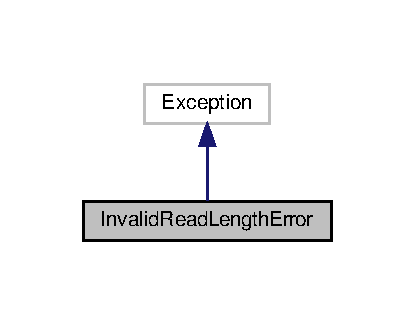
\includegraphics[width=199pt]{classstm__tools_1_1serialflasher_1_1errors_1_1InvalidReadLengthError__inherit__graph}
\end{center}
\end{figure}


Collaboration diagram for Invalid\+Read\+Length\+Error\+:
\nopagebreak
\begin{figure}[H]
\begin{center}
\leavevmode
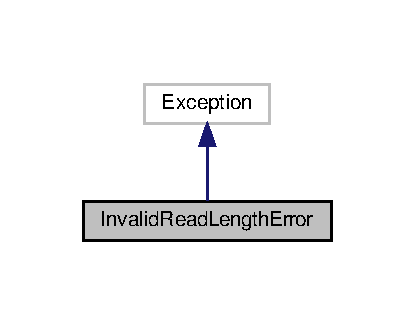
\includegraphics[width=199pt]{classstm__tools_1_1serialflasher_1_1errors_1_1InvalidReadLengthError__coll__graph}
\end{center}
\end{figure}


\subsection{Detailed Description}
\begin{DoxyVerb}the read length is invalid\end{DoxyVerb}
 

The documentation for this class was generated from the following file\+:\begin{DoxyCompactItemize}
\item 
/home/rich/\+Development/\+Py\+Dev/\+S\+T\+M32\+Tools/\+S\+T\+M32\+F1\+\_\+\+Serial\+\_\+\+Flasher/stm\+\_\+tools/serialflasher/\hyperlink{errors_8py}{errors.\+py}\end{DoxyCompactItemize}

\hypertarget{classstm__tools_1_1serialflasher_1_1errors_1_1InvalidResponseLengthError}{}\section{Invalid\+Response\+Length\+Error Class Reference}
\label{classstm__tools_1_1serialflasher_1_1errors_1_1InvalidResponseLengthError}\index{Invalid\+Response\+Length\+Error@{Invalid\+Response\+Length\+Error}}


Inheritance diagram for Invalid\+Response\+Length\+Error\+:
\nopagebreak
\begin{figure}[H]
\begin{center}
\leavevmode
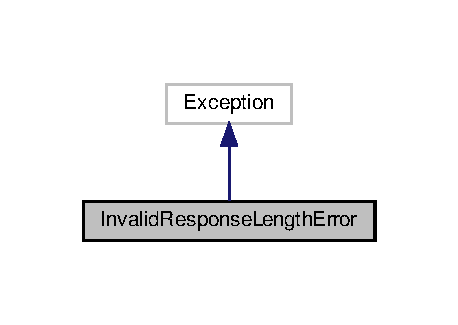
\includegraphics[width=220pt]{classstm__tools_1_1serialflasher_1_1errors_1_1InvalidResponseLengthError__inherit__graph}
\end{center}
\end{figure}


Collaboration diagram for Invalid\+Response\+Length\+Error\+:
\nopagebreak
\begin{figure}[H]
\begin{center}
\leavevmode
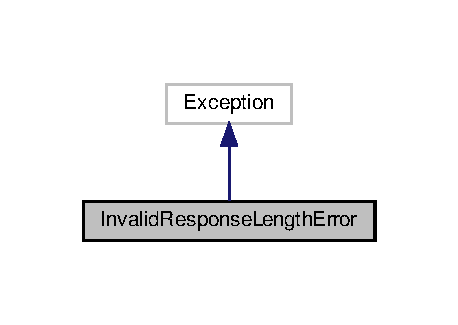
\includegraphics[width=220pt]{classstm__tools_1_1serialflasher_1_1errors_1_1InvalidResponseLengthError__coll__graph}
\end{center}
\end{figure}


\subsection{Detailed Description}
\begin{DoxyVerb}An invalid response length was returned\end{DoxyVerb}
 

The documentation for this class was generated from the following file\+:\begin{DoxyCompactItemize}
\item 
/home/rich/\+Development/\+Py\+Dev/\+S\+T\+M32\+Tools/\+S\+T\+M32\+F1\+\_\+\+Serial\+\_\+\+Flasher/stm\+\_\+tools/serialflasher/\hyperlink{errors_8py}{errors.\+py}\end{DoxyCompactItemize}

\hypertarget{classstm__tools_1_1serialflasher_1_1errors_1_1InvalidWriteLengthError}{}\section{Invalid\+Write\+Length\+Error Class Reference}
\label{classstm__tools_1_1serialflasher_1_1errors_1_1InvalidWriteLengthError}\index{Invalid\+Write\+Length\+Error@{Invalid\+Write\+Length\+Error}}


Inheritance diagram for Invalid\+Write\+Length\+Error\+:
\nopagebreak
\begin{figure}[H]
\begin{center}
\leavevmode
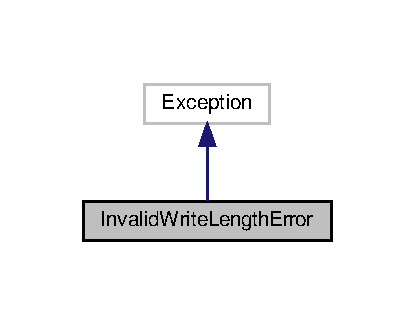
\includegraphics[width=199pt]{classstm__tools_1_1serialflasher_1_1errors_1_1InvalidWriteLengthError__inherit__graph}
\end{center}
\end{figure}


Collaboration diagram for Invalid\+Write\+Length\+Error\+:
\nopagebreak
\begin{figure}[H]
\begin{center}
\leavevmode
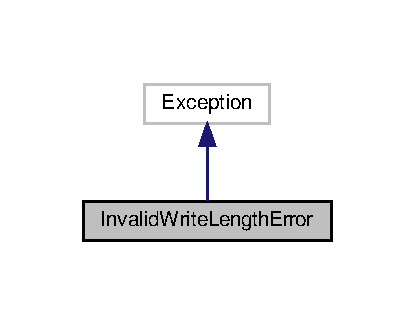
\includegraphics[width=199pt]{classstm__tools_1_1serialflasher_1_1errors_1_1InvalidWriteLengthError__coll__graph}
\end{center}
\end{figure}


\subsection{Detailed Description}
\begin{DoxyVerb}the write length is invalid\end{DoxyVerb}
 

The documentation for this class was generated from the following file\+:\begin{DoxyCompactItemize}
\item 
/home/rich/\+Development/\+Py\+Dev/\+S\+T\+M32\+Tools/\+S\+T\+M32\+F1\+\_\+\+Serial\+\_\+\+Flasher/stm\+\_\+tools/serialflasher/\hyperlink{errors_8py}{errors.\+py}\end{DoxyCompactItemize}

\hypertarget{classstm__tools_1_1serialflasher_1_1errors_1_1NoResponseError}{}\section{No\+Response\+Error Class Reference}
\label{classstm__tools_1_1serialflasher_1_1errors_1_1NoResponseError}\index{No\+Response\+Error@{No\+Response\+Error}}


Inheritance diagram for No\+Response\+Error\+:
\nopagebreak
\begin{figure}[H]
\begin{center}
\leavevmode
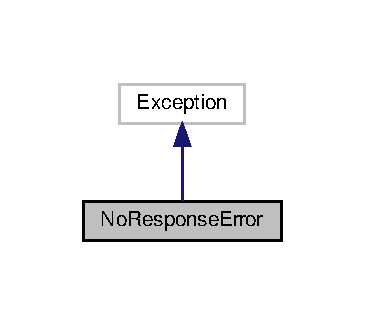
\includegraphics[width=175pt]{classstm__tools_1_1serialflasher_1_1errors_1_1NoResponseError__inherit__graph}
\end{center}
\end{figure}


Collaboration diagram for No\+Response\+Error\+:
\nopagebreak
\begin{figure}[H]
\begin{center}
\leavevmode
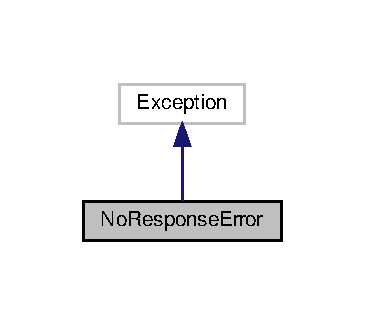
\includegraphics[width=175pt]{classstm__tools_1_1serialflasher_1_1errors_1_1NoResponseError__coll__graph}
\end{center}
\end{figure}


\subsection{Detailed Description}
\begin{DoxyVerb}The device did not respond\end{DoxyVerb}
 

The documentation for this class was generated from the following file\+:\begin{DoxyCompactItemize}
\item 
/home/rich/\+Development/\+Py\+Dev/\+S\+T\+M32\+Tools/\+S\+T\+M32\+F1\+\_\+\+Serial\+\_\+\+Flasher/stm\+\_\+tools/serialflasher/\hyperlink{errors_8py}{errors.\+py}\end{DoxyCompactItemize}

\hypertarget{classstm__tools_1_1tests_1_1optionbytes__test_1_1OptioByteTestCase}{}\section{Optio\+Byte\+Test\+Case Class Reference}
\label{classstm__tools_1_1tests_1_1optionbytes__test_1_1OptioByteTestCase}\index{Optio\+Byte\+Test\+Case@{Optio\+Byte\+Test\+Case}}


Inheritance diagram for Optio\+Byte\+Test\+Case\+:
\nopagebreak
\begin{figure}[H]
\begin{center}
\leavevmode
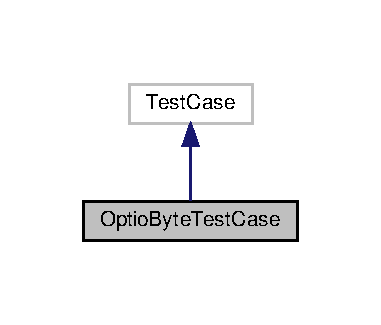
\includegraphics[width=183pt]{classstm__tools_1_1tests_1_1optionbytes__test_1_1OptioByteTestCase__inherit__graph}
\end{center}
\end{figure}


Collaboration diagram for Optio\+Byte\+Test\+Case\+:
\nopagebreak
\begin{figure}[H]
\begin{center}
\leavevmode
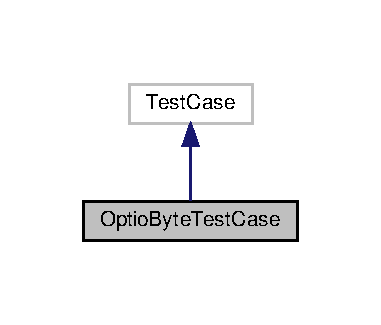
\includegraphics[width=183pt]{classstm__tools_1_1tests_1_1optionbytes__test_1_1OptioByteTestCase__coll__graph}
\end{center}
\end{figure}
\subsection*{Public Member Functions}
\begin{DoxyCompactItemize}
\item 
def \hyperlink{classstm__tools_1_1tests_1_1optionbytes__test_1_1OptioByteTestCase_a52f752f675b44f18235b22d6f574b20e}{test\+Init\+Option\+Bytes\+Attributes\+Instance} (self)
\item 
def \hyperlink{classstm__tools_1_1tests_1_1optionbytes__test_1_1OptioByteTestCase_ad4ac0a0181da1c7c9c4d241c5fc0bde7}{test\+Option\+Bytes\+From\+Bytes\+Instance} (self)
\item 
def \hyperlink{classstm__tools_1_1tests_1_1optionbytes__test_1_1OptioByteTestCase_a3ed58e1144f14d84c4f48d12df377b8b}{test\+Option\+Bytes\+From\+Bytes\+Known\+Data} (self)
\item 
def \hyperlink{classstm__tools_1_1tests_1_1optionbytes__test_1_1OptioByteTestCase_a7c06e67facce403071ee83c0f361e267}{test\+Option\+Bytes\+From\+Attributes\+Known\+Data} (self)
\item 
def \hyperlink{classstm__tools_1_1tests_1_1optionbytes__test_1_1OptioByteTestCase_a24a393387e49294471377b6ffcee128c}{test\+Option\+Bytes\+From\+Attributes\+Known\+Wd\+Type} (self)
\item 
def \hyperlink{classstm__tools_1_1tests_1_1optionbytes__test_1_1OptioByteTestCase_a882a59582b3706a59c616a3c4b8b82f3}{test\+Option\+Bytes\+To\+Bytes\+Method} (self)
\item 
def \hyperlink{classstm__tools_1_1tests_1_1optionbytes__test_1_1OptioByteTestCase_a69fff1f9b79505f64406627efa620f18}{test\+Option\+Bytes\+Resets\+From\+Known} (self)
\item 
def \hyperlink{classstm__tools_1_1tests_1_1optionbytes__test_1_1OptioByteTestCase_ac3a105564c93b8b37a961c9486d72e69}{test\+Option\+Bytes\+Set\+Watchdog\+Type} (self)
\item 
def \hyperlink{classstm__tools_1_1tests_1_1optionbytes__test_1_1OptioByteTestCase_a88cf4703aaf92b596cb9100f5dea70a9}{test\+Option\+Bytes\+Set\+Watchdog\+Value} (self)
\end{DoxyCompactItemize}


\subsection{Member Function Documentation}
\mbox{\Hypertarget{classstm__tools_1_1tests_1_1optionbytes__test_1_1OptioByteTestCase_a52f752f675b44f18235b22d6f574b20e}\label{classstm__tools_1_1tests_1_1optionbytes__test_1_1OptioByteTestCase_a52f752f675b44f18235b22d6f574b20e}} 
\index{stm\+\_\+tools\+::tests\+::optionbytes\+\_\+test\+::\+Optio\+Byte\+Test\+Case@{stm\+\_\+tools\+::tests\+::optionbytes\+\_\+test\+::\+Optio\+Byte\+Test\+Case}!test\+Init\+Option\+Bytes\+Attributes\+Instance@{test\+Init\+Option\+Bytes\+Attributes\+Instance}}
\index{test\+Init\+Option\+Bytes\+Attributes\+Instance@{test\+Init\+Option\+Bytes\+Attributes\+Instance}!stm\+\_\+tools\+::tests\+::optionbytes\+\_\+test\+::\+Optio\+Byte\+Test\+Case@{stm\+\_\+tools\+::tests\+::optionbytes\+\_\+test\+::\+Optio\+Byte\+Test\+Case}}
\subsubsection{\texorpdfstring{test\+Init\+Option\+Bytes\+Attributes\+Instance()}{testInitOptionBytesAttributesInstance()}}
{\footnotesize\ttfamily def test\+Init\+Option\+Bytes\+Attributes\+Instance (\begin{DoxyParamCaption}\item[{}]{self }\end{DoxyParamCaption})}

\mbox{\Hypertarget{classstm__tools_1_1tests_1_1optionbytes__test_1_1OptioByteTestCase_a7c06e67facce403071ee83c0f361e267}\label{classstm__tools_1_1tests_1_1optionbytes__test_1_1OptioByteTestCase_a7c06e67facce403071ee83c0f361e267}} 
\index{stm\+\_\+tools\+::tests\+::optionbytes\+\_\+test\+::\+Optio\+Byte\+Test\+Case@{stm\+\_\+tools\+::tests\+::optionbytes\+\_\+test\+::\+Optio\+Byte\+Test\+Case}!test\+Option\+Bytes\+From\+Attributes\+Known\+Data@{test\+Option\+Bytes\+From\+Attributes\+Known\+Data}}
\index{test\+Option\+Bytes\+From\+Attributes\+Known\+Data@{test\+Option\+Bytes\+From\+Attributes\+Known\+Data}!stm\+\_\+tools\+::tests\+::optionbytes\+\_\+test\+::\+Optio\+Byte\+Test\+Case@{stm\+\_\+tools\+::tests\+::optionbytes\+\_\+test\+::\+Optio\+Byte\+Test\+Case}}
\subsubsection{\texorpdfstring{test\+Option\+Bytes\+From\+Attributes\+Known\+Data()}{testOptionBytesFromAttributesKnownData()}}
{\footnotesize\ttfamily def test\+Option\+Bytes\+From\+Attributes\+Known\+Data (\begin{DoxyParamCaption}\item[{}]{self }\end{DoxyParamCaption})}

\mbox{\Hypertarget{classstm__tools_1_1tests_1_1optionbytes__test_1_1OptioByteTestCase_a24a393387e49294471377b6ffcee128c}\label{classstm__tools_1_1tests_1_1optionbytes__test_1_1OptioByteTestCase_a24a393387e49294471377b6ffcee128c}} 
\index{stm\+\_\+tools\+::tests\+::optionbytes\+\_\+test\+::\+Optio\+Byte\+Test\+Case@{stm\+\_\+tools\+::tests\+::optionbytes\+\_\+test\+::\+Optio\+Byte\+Test\+Case}!test\+Option\+Bytes\+From\+Attributes\+Known\+Wd\+Type@{test\+Option\+Bytes\+From\+Attributes\+Known\+Wd\+Type}}
\index{test\+Option\+Bytes\+From\+Attributes\+Known\+Wd\+Type@{test\+Option\+Bytes\+From\+Attributes\+Known\+Wd\+Type}!stm\+\_\+tools\+::tests\+::optionbytes\+\_\+test\+::\+Optio\+Byte\+Test\+Case@{stm\+\_\+tools\+::tests\+::optionbytes\+\_\+test\+::\+Optio\+Byte\+Test\+Case}}
\subsubsection{\texorpdfstring{test\+Option\+Bytes\+From\+Attributes\+Known\+Wd\+Type()}{testOptionBytesFromAttributesKnownWdType()}}
{\footnotesize\ttfamily def test\+Option\+Bytes\+From\+Attributes\+Known\+Wd\+Type (\begin{DoxyParamCaption}\item[{}]{self }\end{DoxyParamCaption})}

\mbox{\Hypertarget{classstm__tools_1_1tests_1_1optionbytes__test_1_1OptioByteTestCase_ad4ac0a0181da1c7c9c4d241c5fc0bde7}\label{classstm__tools_1_1tests_1_1optionbytes__test_1_1OptioByteTestCase_ad4ac0a0181da1c7c9c4d241c5fc0bde7}} 
\index{stm\+\_\+tools\+::tests\+::optionbytes\+\_\+test\+::\+Optio\+Byte\+Test\+Case@{stm\+\_\+tools\+::tests\+::optionbytes\+\_\+test\+::\+Optio\+Byte\+Test\+Case}!test\+Option\+Bytes\+From\+Bytes\+Instance@{test\+Option\+Bytes\+From\+Bytes\+Instance}}
\index{test\+Option\+Bytes\+From\+Bytes\+Instance@{test\+Option\+Bytes\+From\+Bytes\+Instance}!stm\+\_\+tools\+::tests\+::optionbytes\+\_\+test\+::\+Optio\+Byte\+Test\+Case@{stm\+\_\+tools\+::tests\+::optionbytes\+\_\+test\+::\+Optio\+Byte\+Test\+Case}}
\subsubsection{\texorpdfstring{test\+Option\+Bytes\+From\+Bytes\+Instance()}{testOptionBytesFromBytesInstance()}}
{\footnotesize\ttfamily def test\+Option\+Bytes\+From\+Bytes\+Instance (\begin{DoxyParamCaption}\item[{}]{self }\end{DoxyParamCaption})}

\mbox{\Hypertarget{classstm__tools_1_1tests_1_1optionbytes__test_1_1OptioByteTestCase_a3ed58e1144f14d84c4f48d12df377b8b}\label{classstm__tools_1_1tests_1_1optionbytes__test_1_1OptioByteTestCase_a3ed58e1144f14d84c4f48d12df377b8b}} 
\index{stm\+\_\+tools\+::tests\+::optionbytes\+\_\+test\+::\+Optio\+Byte\+Test\+Case@{stm\+\_\+tools\+::tests\+::optionbytes\+\_\+test\+::\+Optio\+Byte\+Test\+Case}!test\+Option\+Bytes\+From\+Bytes\+Known\+Data@{test\+Option\+Bytes\+From\+Bytes\+Known\+Data}}
\index{test\+Option\+Bytes\+From\+Bytes\+Known\+Data@{test\+Option\+Bytes\+From\+Bytes\+Known\+Data}!stm\+\_\+tools\+::tests\+::optionbytes\+\_\+test\+::\+Optio\+Byte\+Test\+Case@{stm\+\_\+tools\+::tests\+::optionbytes\+\_\+test\+::\+Optio\+Byte\+Test\+Case}}
\subsubsection{\texorpdfstring{test\+Option\+Bytes\+From\+Bytes\+Known\+Data()}{testOptionBytesFromBytesKnownData()}}
{\footnotesize\ttfamily def test\+Option\+Bytes\+From\+Bytes\+Known\+Data (\begin{DoxyParamCaption}\item[{}]{self }\end{DoxyParamCaption})}

\mbox{\Hypertarget{classstm__tools_1_1tests_1_1optionbytes__test_1_1OptioByteTestCase_a69fff1f9b79505f64406627efa620f18}\label{classstm__tools_1_1tests_1_1optionbytes__test_1_1OptioByteTestCase_a69fff1f9b79505f64406627efa620f18}} 
\index{stm\+\_\+tools\+::tests\+::optionbytes\+\_\+test\+::\+Optio\+Byte\+Test\+Case@{stm\+\_\+tools\+::tests\+::optionbytes\+\_\+test\+::\+Optio\+Byte\+Test\+Case}!test\+Option\+Bytes\+Resets\+From\+Known@{test\+Option\+Bytes\+Resets\+From\+Known}}
\index{test\+Option\+Bytes\+Resets\+From\+Known@{test\+Option\+Bytes\+Resets\+From\+Known}!stm\+\_\+tools\+::tests\+::optionbytes\+\_\+test\+::\+Optio\+Byte\+Test\+Case@{stm\+\_\+tools\+::tests\+::optionbytes\+\_\+test\+::\+Optio\+Byte\+Test\+Case}}
\subsubsection{\texorpdfstring{test\+Option\+Bytes\+Resets\+From\+Known()}{testOptionBytesResetsFromKnown()}}
{\footnotesize\ttfamily def test\+Option\+Bytes\+Resets\+From\+Known (\begin{DoxyParamCaption}\item[{}]{self }\end{DoxyParamCaption})}

\mbox{\Hypertarget{classstm__tools_1_1tests_1_1optionbytes__test_1_1OptioByteTestCase_ac3a105564c93b8b37a961c9486d72e69}\label{classstm__tools_1_1tests_1_1optionbytes__test_1_1OptioByteTestCase_ac3a105564c93b8b37a961c9486d72e69}} 
\index{stm\+\_\+tools\+::tests\+::optionbytes\+\_\+test\+::\+Optio\+Byte\+Test\+Case@{stm\+\_\+tools\+::tests\+::optionbytes\+\_\+test\+::\+Optio\+Byte\+Test\+Case}!test\+Option\+Bytes\+Set\+Watchdog\+Type@{test\+Option\+Bytes\+Set\+Watchdog\+Type}}
\index{test\+Option\+Bytes\+Set\+Watchdog\+Type@{test\+Option\+Bytes\+Set\+Watchdog\+Type}!stm\+\_\+tools\+::tests\+::optionbytes\+\_\+test\+::\+Optio\+Byte\+Test\+Case@{stm\+\_\+tools\+::tests\+::optionbytes\+\_\+test\+::\+Optio\+Byte\+Test\+Case}}
\subsubsection{\texorpdfstring{test\+Option\+Bytes\+Set\+Watchdog\+Type()}{testOptionBytesSetWatchdogType()}}
{\footnotesize\ttfamily def test\+Option\+Bytes\+Set\+Watchdog\+Type (\begin{DoxyParamCaption}\item[{}]{self }\end{DoxyParamCaption})}

\mbox{\Hypertarget{classstm__tools_1_1tests_1_1optionbytes__test_1_1OptioByteTestCase_a88cf4703aaf92b596cb9100f5dea70a9}\label{classstm__tools_1_1tests_1_1optionbytes__test_1_1OptioByteTestCase_a88cf4703aaf92b596cb9100f5dea70a9}} 
\index{stm\+\_\+tools\+::tests\+::optionbytes\+\_\+test\+::\+Optio\+Byte\+Test\+Case@{stm\+\_\+tools\+::tests\+::optionbytes\+\_\+test\+::\+Optio\+Byte\+Test\+Case}!test\+Option\+Bytes\+Set\+Watchdog\+Value@{test\+Option\+Bytes\+Set\+Watchdog\+Value}}
\index{test\+Option\+Bytes\+Set\+Watchdog\+Value@{test\+Option\+Bytes\+Set\+Watchdog\+Value}!stm\+\_\+tools\+::tests\+::optionbytes\+\_\+test\+::\+Optio\+Byte\+Test\+Case@{stm\+\_\+tools\+::tests\+::optionbytes\+\_\+test\+::\+Optio\+Byte\+Test\+Case}}
\subsubsection{\texorpdfstring{test\+Option\+Bytes\+Set\+Watchdog\+Value()}{testOptionBytesSetWatchdogValue()}}
{\footnotesize\ttfamily def test\+Option\+Bytes\+Set\+Watchdog\+Value (\begin{DoxyParamCaption}\item[{}]{self }\end{DoxyParamCaption})}

\mbox{\Hypertarget{classstm__tools_1_1tests_1_1optionbytes__test_1_1OptioByteTestCase_a882a59582b3706a59c616a3c4b8b82f3}\label{classstm__tools_1_1tests_1_1optionbytes__test_1_1OptioByteTestCase_a882a59582b3706a59c616a3c4b8b82f3}} 
\index{stm\+\_\+tools\+::tests\+::optionbytes\+\_\+test\+::\+Optio\+Byte\+Test\+Case@{stm\+\_\+tools\+::tests\+::optionbytes\+\_\+test\+::\+Optio\+Byte\+Test\+Case}!test\+Option\+Bytes\+To\+Bytes\+Method@{test\+Option\+Bytes\+To\+Bytes\+Method}}
\index{test\+Option\+Bytes\+To\+Bytes\+Method@{test\+Option\+Bytes\+To\+Bytes\+Method}!stm\+\_\+tools\+::tests\+::optionbytes\+\_\+test\+::\+Optio\+Byte\+Test\+Case@{stm\+\_\+tools\+::tests\+::optionbytes\+\_\+test\+::\+Optio\+Byte\+Test\+Case}}
\subsubsection{\texorpdfstring{test\+Option\+Bytes\+To\+Bytes\+Method()}{testOptionBytesToBytesMethod()}}
{\footnotesize\ttfamily def test\+Option\+Bytes\+To\+Bytes\+Method (\begin{DoxyParamCaption}\item[{}]{self }\end{DoxyParamCaption})}



The documentation for this class was generated from the following file\+:\begin{DoxyCompactItemize}
\item 
/home/rich/\+Development/\+Py\+Dev/\+S\+T\+M32\+Tools/\+S\+T\+M32\+F1\+\_\+\+Serial\+\_\+\+Flasher/stm\+\_\+tools/tests/\hyperlink{optionbytes__test_8py}{optionbytes\+\_\+test.\+py}\end{DoxyCompactItemize}

\hypertarget{classstm__tools_1_1serialflasher_1_1devices_1_1OptionBytes}{}\section{Option\+Bytes Class Reference}
\label{classstm__tools_1_1serialflasher_1_1devices_1_1OptionBytes}\index{Option\+Bytes@{Option\+Bytes}}
\subsection*{Public Member Functions}
\begin{DoxyCompactItemize}
\item 
def \hyperlink{classstm__tools_1_1serialflasher_1_1devices_1_1OptionBytes_ae64f0875afe3067b97ba370b354b9213}{\+\_\+\+\_\+init\+\_\+\+\_\+} (\hyperlink{classstm__tools_1_1serialflasher_1_1devices_1_1OptionBytes_a9a04aa327fd016eb962c5799377e1f29}{self})
\item 
def \hyperlink{classstm__tools_1_1serialflasher_1_1devices_1_1OptionBytes_a382d9cfc8c5960396f6003674cecc20a}{From\+Attributes}
\item 
def \hyperlink{classstm__tools_1_1serialflasher_1_1devices_1_1OptionBytes_aacdb9f5b827de05bfefa79f379a2cd51}{From\+Bytes}
\item 
def \hyperlink{classstm__tools_1_1serialflasher_1_1devices_1_1OptionBytes_aa3e6e65c18eb7dd1ebb4c4988bf67dc3}{generate\+User\+Byte} (\hyperlink{classstm__tools_1_1serialflasher_1_1devices_1_1OptionBytes_a9a04aa327fd016eb962c5799377e1f29}{self})
\item 
def \hyperlink{classstm__tools_1_1serialflasher_1_1devices_1_1OptionBytes_a58a6ff9c9a0a432ab3b19b65c9977a7c}{to\+Bytes} (\hyperlink{classstm__tools_1_1serialflasher_1_1devices_1_1OptionBytes_a9a04aa327fd016eb962c5799377e1f29}{self})
\item 
def \hyperlink{classstm__tools_1_1serialflasher_1_1devices_1_1OptionBytes_ad4f22596222a06b30a766a352adc8c79}{update\+Raw\+Bytes} (\hyperlink{classstm__tools_1_1serialflasher_1_1devices_1_1OptionBytes_a9a04aa327fd016eb962c5799377e1f29}{self})
\item 
def \hyperlink{classstm__tools_1_1serialflasher_1_1devices_1_1OptionBytes_ac529349575475f39414293aade46af32}{raw\+Bytes} (\hyperlink{classstm__tools_1_1serialflasher_1_1devices_1_1OptionBytes_a9a04aa327fd016eb962c5799377e1f29}{self})
\item 
def \hyperlink{classstm__tools_1_1serialflasher_1_1devices_1_1OptionBytes_a54d7cb3878ecd7c655f9267237a72088}{watchdog\+Type} (\hyperlink{classstm__tools_1_1serialflasher_1_1devices_1_1OptionBytes_a9a04aa327fd016eb962c5799377e1f29}{self})
\item 
def \hyperlink{classstm__tools_1_1serialflasher_1_1devices_1_1OptionBytes_a950990256985e0777e404d52930a53a5}{watchdog\+Type}
\item 
def \hyperlink{classstm__tools_1_1serialflasher_1_1devices_1_1OptionBytes_a829d43cd3e895f85115af574e2cf8372}{reset\+On\+Stop} (\hyperlink{classstm__tools_1_1serialflasher_1_1devices_1_1OptionBytes_a9a04aa327fd016eb962c5799377e1f29}{self})
\item 
def \hyperlink{classstm__tools_1_1serialflasher_1_1devices_1_1OptionBytes_a2849d0dc87582555edfbdc691a592c2f}{reset\+On\+Stop}
\item 
def \hyperlink{classstm__tools_1_1serialflasher_1_1devices_1_1OptionBytes_a1084946ed0f38014d2f3089a3e763473}{reset\+On\+Standby} (\hyperlink{classstm__tools_1_1serialflasher_1_1devices_1_1OptionBytes_a9a04aa327fd016eb962c5799377e1f29}{self})
\item 
def \hyperlink{classstm__tools_1_1serialflasher_1_1devices_1_1OptionBytes_af004b4efeda1a23ca9b34e9de37cab5b}{reset\+On\+Standby}
\item 
def \hyperlink{classstm__tools_1_1serialflasher_1_1devices_1_1OptionBytes_a5886e1a7a12ae044368f84aba2b253e7}{data\+Byte0} (\hyperlink{classstm__tools_1_1serialflasher_1_1devices_1_1OptionBytes_a9a04aa327fd016eb962c5799377e1f29}{self})
\item 
def \hyperlink{classstm__tools_1_1serialflasher_1_1devices_1_1OptionBytes_ae3c37f29a1a0045eb7ac5eb21e538b53}{data\+Byte0}
\item 
def \hyperlink{classstm__tools_1_1serialflasher_1_1devices_1_1OptionBytes_a8d3c4f3b019dd028f78d6c1bc8cfa824}{data\+Byte1} (\hyperlink{classstm__tools_1_1serialflasher_1_1devices_1_1OptionBytes_a9a04aa327fd016eb962c5799377e1f29}{self})
\item 
def \hyperlink{classstm__tools_1_1serialflasher_1_1devices_1_1OptionBytes_ae7e2dcb268488f5e5b25938af7d0771c}{data\+Byte1}
\item 
def \hyperlink{classstm__tools_1_1serialflasher_1_1devices_1_1OptionBytes_addf9a0b1e48ed1cf061c6dac3ce933a3}{read\+Protect} (\hyperlink{classstm__tools_1_1serialflasher_1_1devices_1_1OptionBytes_a9a04aa327fd016eb962c5799377e1f29}{self})
\item 
def \hyperlink{classstm__tools_1_1serialflasher_1_1devices_1_1OptionBytes_a1b4d34a5c4f446e466c0b5fb2b0c8acc}{read\+Protect}
\item 
def \hyperlink{classstm__tools_1_1serialflasher_1_1devices_1_1OptionBytes_a560231527be282ea9e401baf676b0b0a}{write\+Protect0} (\hyperlink{classstm__tools_1_1serialflasher_1_1devices_1_1OptionBytes_a9a04aa327fd016eb962c5799377e1f29}{self})
\item 
def \hyperlink{classstm__tools_1_1serialflasher_1_1devices_1_1OptionBytes_a46dcd99862104cc42388a9c6ca8ee249}{write\+Protect0}
\item 
def \hyperlink{classstm__tools_1_1serialflasher_1_1devices_1_1OptionBytes_a9ccf5960bf4062ceeb5106108699fe12}{write\+Protect1} (\hyperlink{classstm__tools_1_1serialflasher_1_1devices_1_1OptionBytes_a9a04aa327fd016eb962c5799377e1f29}{self})
\item 
def \hyperlink{classstm__tools_1_1serialflasher_1_1devices_1_1OptionBytes_aa09ba320b6ac5900dc9539f4eb9adc2e}{write\+Protect1}
\item 
def \hyperlink{classstm__tools_1_1serialflasher_1_1devices_1_1OptionBytes_a6462b4b33a52c1ce10e6104b2ea5d814}{write\+Protect2} (\hyperlink{classstm__tools_1_1serialflasher_1_1devices_1_1OptionBytes_a9a04aa327fd016eb962c5799377e1f29}{self})
\item 
def \hyperlink{classstm__tools_1_1serialflasher_1_1devices_1_1OptionBytes_a1a3b668e419e836a0e0c002ee53c8eb8}{write\+Protect2}
\item 
def \hyperlink{classstm__tools_1_1serialflasher_1_1devices_1_1OptionBytes_a991e45f3f715f40d2893c964ddf622a7}{write\+Protect3} (\hyperlink{classstm__tools_1_1serialflasher_1_1devices_1_1OptionBytes_a9a04aa327fd016eb962c5799377e1f29}{self})
\item 
def \hyperlink{classstm__tools_1_1serialflasher_1_1devices_1_1OptionBytes_a54b1fb61e8c772594a3f655369ca8a01}{write\+Protect3}
\item 
def \hyperlink{classstm__tools_1_1serialflasher_1_1devices_1_1OptionBytes_ab7cc38c038de41730b6656ce9fb2e475}{enable\+Write\+Protect} (\hyperlink{classstm__tools_1_1serialflasher_1_1devices_1_1OptionBytes_a9a04aa327fd016eb962c5799377e1f29}{self})
\item 
def \hyperlink{classstm__tools_1_1serialflasher_1_1devices_1_1OptionBytes_afafad373819bdb9c67312f2d687f5c9d}{disable\+Write\+Protect} (\hyperlink{classstm__tools_1_1serialflasher_1_1devices_1_1OptionBytes_a9a04aa327fd016eb962c5799377e1f29}{self})
\item 
def \hyperlink{classstm__tools_1_1serialflasher_1_1devices_1_1OptionBytes_ab162f97a92cf1ba991d8dd517c3d3357}{dump\+Option\+Bytes} (\hyperlink{classstm__tools_1_1serialflasher_1_1devices_1_1OptionBytes_a9a04aa327fd016eb962c5799377e1f29}{self})
\item 
def \hyperlink{classstm__tools_1_1serialflasher_1_1devices_1_1OptionBytes_a37c60978e654cb0ae2185817163c403d}{raw\+Bytes\+To\+String} (\hyperlink{classstm__tools_1_1serialflasher_1_1devices_1_1OptionBytes_a9a04aa327fd016eb962c5799377e1f29}{self})
\end{DoxyCompactItemize}
\subsection*{Static Public Attributes}
\begin{DoxyCompactItemize}
\item 
\hyperlink{classstm__tools_1_1serialflasher_1_1devices_1_1OptionBytes_a61569f2965b7a369eb10b6d75d410d11}{int}
\item 
\hyperlink{classstm__tools_1_1serialflasher_1_1devices_1_1OptionBytes_a50d56d469cf437646fbb6d0c63ba7e9e}{bytearray}
\item 
\hyperlink{classstm__tools_1_1serialflasher_1_1devices_1_1OptionBytes_a9a04aa327fd016eb962c5799377e1f29}{self}
\item 
\hyperlink{classstm__tools_1_1serialflasher_1_1devices_1_1OptionBytes_a099b94c6be2822f849135ae50e806b73}{read\+\_\+protect}
\item 
\hyperlink{classstm__tools_1_1serialflasher_1_1devices_1_1OptionBytes_a352ca3d6460ffb8b4be71ca5b2b4a66a}{watchdog\+\_\+type}
\item 
\hyperlink{classstm__tools_1_1serialflasher_1_1devices_1_1OptionBytes_a563f83e9bb0cc532cb6c29efa34fc212}{reset\+\_\+on\+\_\+stop}
\item 
\hyperlink{classstm__tools_1_1serialflasher_1_1devices_1_1OptionBytes_af6b8cda6e2e17ec7cedeb961272d8f95}{reset\+\_\+on\+\_\+standby}
\item 
\hyperlink{classstm__tools_1_1serialflasher_1_1devices_1_1OptionBytes_a5cc32e366c87c4cb49e4309b75f57d64}{user}
\item 
\hyperlink{classstm__tools_1_1serialflasher_1_1devices_1_1OptionBytes_aa26ed87f84ce36929a443c5ca5ab883e}{data\+\_\+byte\+\_\+0}
\item 
\hyperlink{classstm__tools_1_1serialflasher_1_1devices_1_1OptionBytes_a55f7b4672c91d43b12e6e6fa50ae0078}{data\+\_\+byte\+\_\+1}
\item 
\hyperlink{classstm__tools_1_1serialflasher_1_1devices_1_1OptionBytes_aa6d5a8bc15ad2248eca0c8db3281bb10}{write\+\_\+protect\+\_\+0}
\item 
\hyperlink{classstm__tools_1_1serialflasher_1_1devices_1_1OptionBytes_a8ff355caabcc05c7a12d63948443db25}{write\+\_\+protect\+\_\+1}
\item 
\hyperlink{classstm__tools_1_1serialflasher_1_1devices_1_1OptionBytes_aec7190b83930f8f9e716ec1f07333eab}{write\+\_\+protect\+\_\+2}
\item 
\hyperlink{classstm__tools_1_1serialflasher_1_1devices_1_1OptionBytes_a728da06e5068901f3524fe02a873e514}{write\+\_\+protect\+\_\+3}
\item 
\hyperlink{classstm__tools_1_1serialflasher_1_1devices_1_1OptionBytes_a55a904d43455b0d4484caa720e744a83}{raw\+\_\+bytes}
\end{DoxyCompactItemize}


\subsection{Detailed Description}
\begin{DoxyVerb}enough messing about with tuples
make a proper class with functionality
and stuff. This might have got out of control.
But it's almost worth it if only for the practice
\end{DoxyVerb}
 

\subsection{Constructor \& Destructor Documentation}
\mbox{\Hypertarget{classstm__tools_1_1serialflasher_1_1devices_1_1OptionBytes_ae64f0875afe3067b97ba370b354b9213}\label{classstm__tools_1_1serialflasher_1_1devices_1_1OptionBytes_ae64f0875afe3067b97ba370b354b9213}} 
\index{stm\+\_\+tools\+::serialflasher\+::devices\+::\+Option\+Bytes@{stm\+\_\+tools\+::serialflasher\+::devices\+::\+Option\+Bytes}!\+\_\+\+\_\+init\+\_\+\+\_\+@{\+\_\+\+\_\+init\+\_\+\+\_\+}}
\index{\+\_\+\+\_\+init\+\_\+\+\_\+@{\+\_\+\+\_\+init\+\_\+\+\_\+}!stm\+\_\+tools\+::serialflasher\+::devices\+::\+Option\+Bytes@{stm\+\_\+tools\+::serialflasher\+::devices\+::\+Option\+Bytes}}
\subsubsection{\texorpdfstring{\+\_\+\+\_\+init\+\_\+\+\_\+()}{\_\_init\_\_()}}
{\footnotesize\ttfamily def \+\_\+\+\_\+init\+\_\+\+\_\+ (\begin{DoxyParamCaption}\item[{}]{self }\end{DoxyParamCaption})}

\begin{DoxyVerb}Default Constructor - do not use.\end{DoxyVerb}
 

\subsection{Member Function Documentation}
\mbox{\Hypertarget{classstm__tools_1_1serialflasher_1_1devices_1_1OptionBytes_a5886e1a7a12ae044368f84aba2b253e7}\label{classstm__tools_1_1serialflasher_1_1devices_1_1OptionBytes_a5886e1a7a12ae044368f84aba2b253e7}} 
\index{stm\+\_\+tools\+::serialflasher\+::devices\+::\+Option\+Bytes@{stm\+\_\+tools\+::serialflasher\+::devices\+::\+Option\+Bytes}!data\+Byte0@{data\+Byte0}}
\index{data\+Byte0@{data\+Byte0}!stm\+\_\+tools\+::serialflasher\+::devices\+::\+Option\+Bytes@{stm\+\_\+tools\+::serialflasher\+::devices\+::\+Option\+Bytes}}
\subsubsection{\texorpdfstring{data\+Byte0()}{dataByte0()}\hspace{0.1cm}{\footnotesize\ttfamily [1/2]}}
{\footnotesize\ttfamily def data\+Byte0 (\begin{DoxyParamCaption}\item[{}]{self,  }\item[{}]{int }\end{DoxyParamCaption})}

\begin{DoxyVerb}_summary_

Returns:
    int: data byte 0 value
\end{DoxyVerb}
 \mbox{\Hypertarget{classstm__tools_1_1serialflasher_1_1devices_1_1OptionBytes_ae3c37f29a1a0045eb7ac5eb21e538b53}\label{classstm__tools_1_1serialflasher_1_1devices_1_1OptionBytes_ae3c37f29a1a0045eb7ac5eb21e538b53}} 
\index{stm\+\_\+tools\+::serialflasher\+::devices\+::\+Option\+Bytes@{stm\+\_\+tools\+::serialflasher\+::devices\+::\+Option\+Bytes}!data\+Byte0@{data\+Byte0}}
\index{data\+Byte0@{data\+Byte0}!stm\+\_\+tools\+::serialflasher\+::devices\+::\+Option\+Bytes@{stm\+\_\+tools\+::serialflasher\+::devices\+::\+Option\+Bytes}}
\subsubsection{\texorpdfstring{data\+Byte0()}{dataByte0()}\hspace{0.1cm}{\footnotesize\ttfamily [2/2]}}
{\footnotesize\ttfamily def data\+Byte0 (\begin{DoxyParamCaption}\item[{}]{self,  }\item[{}]{data }\end{DoxyParamCaption})}

\mbox{\Hypertarget{classstm__tools_1_1serialflasher_1_1devices_1_1OptionBytes_a8d3c4f3b019dd028f78d6c1bc8cfa824}\label{classstm__tools_1_1serialflasher_1_1devices_1_1OptionBytes_a8d3c4f3b019dd028f78d6c1bc8cfa824}} 
\index{stm\+\_\+tools\+::serialflasher\+::devices\+::\+Option\+Bytes@{stm\+\_\+tools\+::serialflasher\+::devices\+::\+Option\+Bytes}!data\+Byte1@{data\+Byte1}}
\index{data\+Byte1@{data\+Byte1}!stm\+\_\+tools\+::serialflasher\+::devices\+::\+Option\+Bytes@{stm\+\_\+tools\+::serialflasher\+::devices\+::\+Option\+Bytes}}
\subsubsection{\texorpdfstring{data\+Byte1()}{dataByte1()}\hspace{0.1cm}{\footnotesize\ttfamily [1/2]}}
{\footnotesize\ttfamily def data\+Byte1 (\begin{DoxyParamCaption}\item[{}]{self }\end{DoxyParamCaption})}

\mbox{\Hypertarget{classstm__tools_1_1serialflasher_1_1devices_1_1OptionBytes_ae7e2dcb268488f5e5b25938af7d0771c}\label{classstm__tools_1_1serialflasher_1_1devices_1_1OptionBytes_ae7e2dcb268488f5e5b25938af7d0771c}} 
\index{stm\+\_\+tools\+::serialflasher\+::devices\+::\+Option\+Bytes@{stm\+\_\+tools\+::serialflasher\+::devices\+::\+Option\+Bytes}!data\+Byte1@{data\+Byte1}}
\index{data\+Byte1@{data\+Byte1}!stm\+\_\+tools\+::serialflasher\+::devices\+::\+Option\+Bytes@{stm\+\_\+tools\+::serialflasher\+::devices\+::\+Option\+Bytes}}
\subsubsection{\texorpdfstring{data\+Byte1()}{dataByte1()}\hspace{0.1cm}{\footnotesize\ttfamily [2/2]}}
{\footnotesize\ttfamily def data\+Byte1 (\begin{DoxyParamCaption}\item[{}]{self,  }\item[{}]{data }\end{DoxyParamCaption})}

\mbox{\Hypertarget{classstm__tools_1_1serialflasher_1_1devices_1_1OptionBytes_afafad373819bdb9c67312f2d687f5c9d}\label{classstm__tools_1_1serialflasher_1_1devices_1_1OptionBytes_afafad373819bdb9c67312f2d687f5c9d}} 
\index{stm\+\_\+tools\+::serialflasher\+::devices\+::\+Option\+Bytes@{stm\+\_\+tools\+::serialflasher\+::devices\+::\+Option\+Bytes}!disable\+Write\+Protect@{disable\+Write\+Protect}}
\index{disable\+Write\+Protect@{disable\+Write\+Protect}!stm\+\_\+tools\+::serialflasher\+::devices\+::\+Option\+Bytes@{stm\+\_\+tools\+::serialflasher\+::devices\+::\+Option\+Bytes}}
\subsubsection{\texorpdfstring{disable\+Write\+Protect()}{disableWriteProtect()}}
{\footnotesize\ttfamily def disable\+Write\+Protect (\begin{DoxyParamCaption}\item[{}]{self }\end{DoxyParamCaption})}

\mbox{\Hypertarget{classstm__tools_1_1serialflasher_1_1devices_1_1OptionBytes_ab162f97a92cf1ba991d8dd517c3d3357}\label{classstm__tools_1_1serialflasher_1_1devices_1_1OptionBytes_ab162f97a92cf1ba991d8dd517c3d3357}} 
\index{stm\+\_\+tools\+::serialflasher\+::devices\+::\+Option\+Bytes@{stm\+\_\+tools\+::serialflasher\+::devices\+::\+Option\+Bytes}!dump\+Option\+Bytes@{dump\+Option\+Bytes}}
\index{dump\+Option\+Bytes@{dump\+Option\+Bytes}!stm\+\_\+tools\+::serialflasher\+::devices\+::\+Option\+Bytes@{stm\+\_\+tools\+::serialflasher\+::devices\+::\+Option\+Bytes}}
\subsubsection{\texorpdfstring{dump\+Option\+Bytes()}{dumpOptionBytes()}}
{\footnotesize\ttfamily def dump\+Option\+Bytes (\begin{DoxyParamCaption}\item[{}]{self }\end{DoxyParamCaption})}

\mbox{\Hypertarget{classstm__tools_1_1serialflasher_1_1devices_1_1OptionBytes_ab7cc38c038de41730b6656ce9fb2e475}\label{classstm__tools_1_1serialflasher_1_1devices_1_1OptionBytes_ab7cc38c038de41730b6656ce9fb2e475}} 
\index{stm\+\_\+tools\+::serialflasher\+::devices\+::\+Option\+Bytes@{stm\+\_\+tools\+::serialflasher\+::devices\+::\+Option\+Bytes}!enable\+Write\+Protect@{enable\+Write\+Protect}}
\index{enable\+Write\+Protect@{enable\+Write\+Protect}!stm\+\_\+tools\+::serialflasher\+::devices\+::\+Option\+Bytes@{stm\+\_\+tools\+::serialflasher\+::devices\+::\+Option\+Bytes}}
\subsubsection{\texorpdfstring{enable\+Write\+Protect()}{enableWriteProtect()}}
{\footnotesize\ttfamily def enable\+Write\+Protect (\begin{DoxyParamCaption}\item[{}]{self }\end{DoxyParamCaption})}

\mbox{\Hypertarget{classstm__tools_1_1serialflasher_1_1devices_1_1OptionBytes_a382d9cfc8c5960396f6003674cecc20a}\label{classstm__tools_1_1serialflasher_1_1devices_1_1OptionBytes_a382d9cfc8c5960396f6003674cecc20a}} 
\index{stm\+\_\+tools\+::serialflasher\+::devices\+::\+Option\+Bytes@{stm\+\_\+tools\+::serialflasher\+::devices\+::\+Option\+Bytes}!From\+Attributes@{From\+Attributes}}
\index{From\+Attributes@{From\+Attributes}!stm\+\_\+tools\+::serialflasher\+::devices\+::\+Option\+Bytes@{stm\+\_\+tools\+::serialflasher\+::devices\+::\+Option\+Bytes}}
\subsubsection{\texorpdfstring{From\+Attributes()}{FromAttributes()}}
{\footnotesize\ttfamily def From\+Attributes (\begin{DoxyParamCaption}\item[{}]{cls,  }\item[{}]{read\+\_\+protect }\end{DoxyParamCaption})}

\mbox{\Hypertarget{classstm__tools_1_1serialflasher_1_1devices_1_1OptionBytes_aacdb9f5b827de05bfefa79f379a2cd51}\label{classstm__tools_1_1serialflasher_1_1devices_1_1OptionBytes_aacdb9f5b827de05bfefa79f379a2cd51}} 
\index{stm\+\_\+tools\+::serialflasher\+::devices\+::\+Option\+Bytes@{stm\+\_\+tools\+::serialflasher\+::devices\+::\+Option\+Bytes}!From\+Bytes@{From\+Bytes}}
\index{From\+Bytes@{From\+Bytes}!stm\+\_\+tools\+::serialflasher\+::devices\+::\+Option\+Bytes@{stm\+\_\+tools\+::serialflasher\+::devices\+::\+Option\+Bytes}}
\subsubsection{\texorpdfstring{From\+Bytes()}{FromBytes()}}
{\footnotesize\ttfamily def From\+Bytes (\begin{DoxyParamCaption}\item[{}]{cls,  }\item[{}]{data }\end{DoxyParamCaption})}

\mbox{\Hypertarget{classstm__tools_1_1serialflasher_1_1devices_1_1OptionBytes_aa3e6e65c18eb7dd1ebb4c4988bf67dc3}\label{classstm__tools_1_1serialflasher_1_1devices_1_1OptionBytes_aa3e6e65c18eb7dd1ebb4c4988bf67dc3}} 
\index{stm\+\_\+tools\+::serialflasher\+::devices\+::\+Option\+Bytes@{stm\+\_\+tools\+::serialflasher\+::devices\+::\+Option\+Bytes}!generate\+User\+Byte@{generate\+User\+Byte}}
\index{generate\+User\+Byte@{generate\+User\+Byte}!stm\+\_\+tools\+::serialflasher\+::devices\+::\+Option\+Bytes@{stm\+\_\+tools\+::serialflasher\+::devices\+::\+Option\+Bytes}}
\subsubsection{\texorpdfstring{generate\+User\+Byte()}{generateUserByte()}}
{\footnotesize\ttfamily def generate\+User\+Byte (\begin{DoxyParamCaption}\item[{}]{self,  }\item[{}]{int }\end{DoxyParamCaption})}

\begin{DoxyVerb}generate the user-byte from watchdog and reset settings

Returns:
    int: assembled user-byte
\end{DoxyVerb}
 \mbox{\Hypertarget{classstm__tools_1_1serialflasher_1_1devices_1_1OptionBytes_ac529349575475f39414293aade46af32}\label{classstm__tools_1_1serialflasher_1_1devices_1_1OptionBytes_ac529349575475f39414293aade46af32}} 
\index{stm\+\_\+tools\+::serialflasher\+::devices\+::\+Option\+Bytes@{stm\+\_\+tools\+::serialflasher\+::devices\+::\+Option\+Bytes}!raw\+Bytes@{raw\+Bytes}}
\index{raw\+Bytes@{raw\+Bytes}!stm\+\_\+tools\+::serialflasher\+::devices\+::\+Option\+Bytes@{stm\+\_\+tools\+::serialflasher\+::devices\+::\+Option\+Bytes}}
\subsubsection{\texorpdfstring{raw\+Bytes()}{rawBytes()}}
{\footnotesize\ttfamily def raw\+Bytes (\begin{DoxyParamCaption}\item[{}]{self,  }\item[{}]{bytearray }\end{DoxyParamCaption})}

\begin{DoxyVerb}raw bytes getter

Returns:
    bytearray: option bytes as 16-byte array
\end{DoxyVerb}
 \mbox{\Hypertarget{classstm__tools_1_1serialflasher_1_1devices_1_1OptionBytes_a37c60978e654cb0ae2185817163c403d}\label{classstm__tools_1_1serialflasher_1_1devices_1_1OptionBytes_a37c60978e654cb0ae2185817163c403d}} 
\index{stm\+\_\+tools\+::serialflasher\+::devices\+::\+Option\+Bytes@{stm\+\_\+tools\+::serialflasher\+::devices\+::\+Option\+Bytes}!raw\+Bytes\+To\+String@{raw\+Bytes\+To\+String}}
\index{raw\+Bytes\+To\+String@{raw\+Bytes\+To\+String}!stm\+\_\+tools\+::serialflasher\+::devices\+::\+Option\+Bytes@{stm\+\_\+tools\+::serialflasher\+::devices\+::\+Option\+Bytes}}
\subsubsection{\texorpdfstring{raw\+Bytes\+To\+String()}{rawBytesToString()}}
{\footnotesize\ttfamily def raw\+Bytes\+To\+String (\begin{DoxyParamCaption}\item[{}]{self }\end{DoxyParamCaption})}

\mbox{\Hypertarget{classstm__tools_1_1serialflasher_1_1devices_1_1OptionBytes_addf9a0b1e48ed1cf061c6dac3ce933a3}\label{classstm__tools_1_1serialflasher_1_1devices_1_1OptionBytes_addf9a0b1e48ed1cf061c6dac3ce933a3}} 
\index{stm\+\_\+tools\+::serialflasher\+::devices\+::\+Option\+Bytes@{stm\+\_\+tools\+::serialflasher\+::devices\+::\+Option\+Bytes}!read\+Protect@{read\+Protect}}
\index{read\+Protect@{read\+Protect}!stm\+\_\+tools\+::serialflasher\+::devices\+::\+Option\+Bytes@{stm\+\_\+tools\+::serialflasher\+::devices\+::\+Option\+Bytes}}
\subsubsection{\texorpdfstring{read\+Protect()}{readProtect()}\hspace{0.1cm}{\footnotesize\ttfamily [1/2]}}
{\footnotesize\ttfamily def read\+Protect (\begin{DoxyParamCaption}\item[{}]{self,  }\item[{}]{bool }\end{DoxyParamCaption})}

\mbox{\Hypertarget{classstm__tools_1_1serialflasher_1_1devices_1_1OptionBytes_a1b4d34a5c4f446e466c0b5fb2b0c8acc}\label{classstm__tools_1_1serialflasher_1_1devices_1_1OptionBytes_a1b4d34a5c4f446e466c0b5fb2b0c8acc}} 
\index{stm\+\_\+tools\+::serialflasher\+::devices\+::\+Option\+Bytes@{stm\+\_\+tools\+::serialflasher\+::devices\+::\+Option\+Bytes}!read\+Protect@{read\+Protect}}
\index{read\+Protect@{read\+Protect}!stm\+\_\+tools\+::serialflasher\+::devices\+::\+Option\+Bytes@{stm\+\_\+tools\+::serialflasher\+::devices\+::\+Option\+Bytes}}
\subsubsection{\texorpdfstring{read\+Protect()}{readProtect()}\hspace{0.1cm}{\footnotesize\ttfamily [2/2]}}
{\footnotesize\ttfamily def read\+Protect (\begin{DoxyParamCaption}\item[{}]{self,  }\item[{}]{enabled }\end{DoxyParamCaption})}

\mbox{\Hypertarget{classstm__tools_1_1serialflasher_1_1devices_1_1OptionBytes_a1084946ed0f38014d2f3089a3e763473}\label{classstm__tools_1_1serialflasher_1_1devices_1_1OptionBytes_a1084946ed0f38014d2f3089a3e763473}} 
\index{stm\+\_\+tools\+::serialflasher\+::devices\+::\+Option\+Bytes@{stm\+\_\+tools\+::serialflasher\+::devices\+::\+Option\+Bytes}!reset\+On\+Standby@{reset\+On\+Standby}}
\index{reset\+On\+Standby@{reset\+On\+Standby}!stm\+\_\+tools\+::serialflasher\+::devices\+::\+Option\+Bytes@{stm\+\_\+tools\+::serialflasher\+::devices\+::\+Option\+Bytes}}
\subsubsection{\texorpdfstring{reset\+On\+Standby()}{resetOnStandby()}\hspace{0.1cm}{\footnotesize\ttfamily [1/2]}}
{\footnotesize\ttfamily def reset\+On\+Standby (\begin{DoxyParamCaption}\item[{}]{self,  }\item[{}]{bool }\end{DoxyParamCaption})}

\begin{DoxyVerb}get reset on standby setting
Returns:
    bool: reset on standby enabled
\end{DoxyVerb}
 \mbox{\Hypertarget{classstm__tools_1_1serialflasher_1_1devices_1_1OptionBytes_af004b4efeda1a23ca9b34e9de37cab5b}\label{classstm__tools_1_1serialflasher_1_1devices_1_1OptionBytes_af004b4efeda1a23ca9b34e9de37cab5b}} 
\index{stm\+\_\+tools\+::serialflasher\+::devices\+::\+Option\+Bytes@{stm\+\_\+tools\+::serialflasher\+::devices\+::\+Option\+Bytes}!reset\+On\+Standby@{reset\+On\+Standby}}
\index{reset\+On\+Standby@{reset\+On\+Standby}!stm\+\_\+tools\+::serialflasher\+::devices\+::\+Option\+Bytes@{stm\+\_\+tools\+::serialflasher\+::devices\+::\+Option\+Bytes}}
\subsubsection{\texorpdfstring{reset\+On\+Standby()}{resetOnStandby()}\hspace{0.1cm}{\footnotesize\ttfamily [2/2]}}
{\footnotesize\ttfamily def reset\+On\+Standby (\begin{DoxyParamCaption}\item[{}]{self,  }\item[{}]{ros }\end{DoxyParamCaption})}

\mbox{\Hypertarget{classstm__tools_1_1serialflasher_1_1devices_1_1OptionBytes_a829d43cd3e895f85115af574e2cf8372}\label{classstm__tools_1_1serialflasher_1_1devices_1_1OptionBytes_a829d43cd3e895f85115af574e2cf8372}} 
\index{stm\+\_\+tools\+::serialflasher\+::devices\+::\+Option\+Bytes@{stm\+\_\+tools\+::serialflasher\+::devices\+::\+Option\+Bytes}!reset\+On\+Stop@{reset\+On\+Stop}}
\index{reset\+On\+Stop@{reset\+On\+Stop}!stm\+\_\+tools\+::serialflasher\+::devices\+::\+Option\+Bytes@{stm\+\_\+tools\+::serialflasher\+::devices\+::\+Option\+Bytes}}
\subsubsection{\texorpdfstring{reset\+On\+Stop()}{resetOnStop()}\hspace{0.1cm}{\footnotesize\ttfamily [1/2]}}
{\footnotesize\ttfamily def reset\+On\+Stop (\begin{DoxyParamCaption}\item[{}]{self,  }\item[{}]{int }\end{DoxyParamCaption})}

\begin{DoxyVerb}reset on stop getter

Returns:
    int: reset on stop enabled
\end{DoxyVerb}
 \mbox{\Hypertarget{classstm__tools_1_1serialflasher_1_1devices_1_1OptionBytes_a2849d0dc87582555edfbdc691a592c2f}\label{classstm__tools_1_1serialflasher_1_1devices_1_1OptionBytes_a2849d0dc87582555edfbdc691a592c2f}} 
\index{stm\+\_\+tools\+::serialflasher\+::devices\+::\+Option\+Bytes@{stm\+\_\+tools\+::serialflasher\+::devices\+::\+Option\+Bytes}!reset\+On\+Stop@{reset\+On\+Stop}}
\index{reset\+On\+Stop@{reset\+On\+Stop}!stm\+\_\+tools\+::serialflasher\+::devices\+::\+Option\+Bytes@{stm\+\_\+tools\+::serialflasher\+::devices\+::\+Option\+Bytes}}
\subsubsection{\texorpdfstring{reset\+On\+Stop()}{resetOnStop()}\hspace{0.1cm}{\footnotesize\ttfamily [2/2]}}
{\footnotesize\ttfamily def reset\+On\+Stop (\begin{DoxyParamCaption}\item[{}]{self,  }\item[{}]{ros }\end{DoxyParamCaption})}

\mbox{\Hypertarget{classstm__tools_1_1serialflasher_1_1devices_1_1OptionBytes_a58a6ff9c9a0a432ab3b19b65c9977a7c}\label{classstm__tools_1_1serialflasher_1_1devices_1_1OptionBytes_a58a6ff9c9a0a432ab3b19b65c9977a7c}} 
\index{stm\+\_\+tools\+::serialflasher\+::devices\+::\+Option\+Bytes@{stm\+\_\+tools\+::serialflasher\+::devices\+::\+Option\+Bytes}!to\+Bytes@{to\+Bytes}}
\index{to\+Bytes@{to\+Bytes}!stm\+\_\+tools\+::serialflasher\+::devices\+::\+Option\+Bytes@{stm\+\_\+tools\+::serialflasher\+::devices\+::\+Option\+Bytes}}
\subsubsection{\texorpdfstring{to\+Bytes()}{toBytes()}}
{\footnotesize\ttfamily def to\+Bytes (\begin{DoxyParamCaption}\item[{}]{self,  }\item[{}]{bytearray }\end{DoxyParamCaption})}

\begin{DoxyVerb}generate option bytes as raw bytes from attributes

Returns:
    bytearray: raw bytes
\end{DoxyVerb}
 \mbox{\Hypertarget{classstm__tools_1_1serialflasher_1_1devices_1_1OptionBytes_ad4f22596222a06b30a766a352adc8c79}\label{classstm__tools_1_1serialflasher_1_1devices_1_1OptionBytes_ad4f22596222a06b30a766a352adc8c79}} 
\index{stm\+\_\+tools\+::serialflasher\+::devices\+::\+Option\+Bytes@{stm\+\_\+tools\+::serialflasher\+::devices\+::\+Option\+Bytes}!update\+Raw\+Bytes@{update\+Raw\+Bytes}}
\index{update\+Raw\+Bytes@{update\+Raw\+Bytes}!stm\+\_\+tools\+::serialflasher\+::devices\+::\+Option\+Bytes@{stm\+\_\+tools\+::serialflasher\+::devices\+::\+Option\+Bytes}}
\subsubsection{\texorpdfstring{update\+Raw\+Bytes()}{updateRawBytes()}}
{\footnotesize\ttfamily def update\+Raw\+Bytes (\begin{DoxyParamCaption}\item[{}]{self,  }\item[{}]{None }\end{DoxyParamCaption})}

\begin{DoxyVerb}updates the raw bytes attribute from self attributes\end{DoxyVerb}
 \mbox{\Hypertarget{classstm__tools_1_1serialflasher_1_1devices_1_1OptionBytes_a54d7cb3878ecd7c655f9267237a72088}\label{classstm__tools_1_1serialflasher_1_1devices_1_1OptionBytes_a54d7cb3878ecd7c655f9267237a72088}} 
\index{stm\+\_\+tools\+::serialflasher\+::devices\+::\+Option\+Bytes@{stm\+\_\+tools\+::serialflasher\+::devices\+::\+Option\+Bytes}!watchdog\+Type@{watchdog\+Type}}
\index{watchdog\+Type@{watchdog\+Type}!stm\+\_\+tools\+::serialflasher\+::devices\+::\+Option\+Bytes@{stm\+\_\+tools\+::serialflasher\+::devices\+::\+Option\+Bytes}}
\subsubsection{\texorpdfstring{watchdog\+Type()}{watchdogType()}\hspace{0.1cm}{\footnotesize\ttfamily [1/2]}}
{\footnotesize\ttfamily def watchdog\+Type (\begin{DoxyParamCaption}\item[{}]{self,  }\item[{}]{int }\end{DoxyParamCaption})}

\begin{DoxyVerb}getter for watchdog type
    TODO: Fix this as a variable type - don't mix
    bool/int in getter/setter!

Returns:
    int: watchdog type
\end{DoxyVerb}
 \mbox{\Hypertarget{classstm__tools_1_1serialflasher_1_1devices_1_1OptionBytes_a950990256985e0777e404d52930a53a5}\label{classstm__tools_1_1serialflasher_1_1devices_1_1OptionBytes_a950990256985e0777e404d52930a53a5}} 
\index{stm\+\_\+tools\+::serialflasher\+::devices\+::\+Option\+Bytes@{stm\+\_\+tools\+::serialflasher\+::devices\+::\+Option\+Bytes}!watchdog\+Type@{watchdog\+Type}}
\index{watchdog\+Type@{watchdog\+Type}!stm\+\_\+tools\+::serialflasher\+::devices\+::\+Option\+Bytes@{stm\+\_\+tools\+::serialflasher\+::devices\+::\+Option\+Bytes}}
\subsubsection{\texorpdfstring{watchdog\+Type()}{watchdogType()}\hspace{0.1cm}{\footnotesize\ttfamily [2/2]}}
{\footnotesize\ttfamily def watchdog\+Type (\begin{DoxyParamCaption}\item[{}]{self,  }\item[{}]{watchdog\+\_\+type }\end{DoxyParamCaption})}

\mbox{\Hypertarget{classstm__tools_1_1serialflasher_1_1devices_1_1OptionBytes_a560231527be282ea9e401baf676b0b0a}\label{classstm__tools_1_1serialflasher_1_1devices_1_1OptionBytes_a560231527be282ea9e401baf676b0b0a}} 
\index{stm\+\_\+tools\+::serialflasher\+::devices\+::\+Option\+Bytes@{stm\+\_\+tools\+::serialflasher\+::devices\+::\+Option\+Bytes}!write\+Protect0@{write\+Protect0}}
\index{write\+Protect0@{write\+Protect0}!stm\+\_\+tools\+::serialflasher\+::devices\+::\+Option\+Bytes@{stm\+\_\+tools\+::serialflasher\+::devices\+::\+Option\+Bytes}}
\subsubsection{\texorpdfstring{write\+Protect0()}{writeProtect0()}\hspace{0.1cm}{\footnotesize\ttfamily [1/2]}}
{\footnotesize\ttfamily def write\+Protect0 (\begin{DoxyParamCaption}\item[{}]{self }\end{DoxyParamCaption})}

\mbox{\Hypertarget{classstm__tools_1_1serialflasher_1_1devices_1_1OptionBytes_a46dcd99862104cc42388a9c6ca8ee249}\label{classstm__tools_1_1serialflasher_1_1devices_1_1OptionBytes_a46dcd99862104cc42388a9c6ca8ee249}} 
\index{stm\+\_\+tools\+::serialflasher\+::devices\+::\+Option\+Bytes@{stm\+\_\+tools\+::serialflasher\+::devices\+::\+Option\+Bytes}!write\+Protect0@{write\+Protect0}}
\index{write\+Protect0@{write\+Protect0}!stm\+\_\+tools\+::serialflasher\+::devices\+::\+Option\+Bytes@{stm\+\_\+tools\+::serialflasher\+::devices\+::\+Option\+Bytes}}
\subsubsection{\texorpdfstring{write\+Protect0()}{writeProtect0()}\hspace{0.1cm}{\footnotesize\ttfamily [2/2]}}
{\footnotesize\ttfamily def write\+Protect0 (\begin{DoxyParamCaption}\item[{}]{self,  }\item[{}]{data }\end{DoxyParamCaption})}

\mbox{\Hypertarget{classstm__tools_1_1serialflasher_1_1devices_1_1OptionBytes_a9ccf5960bf4062ceeb5106108699fe12}\label{classstm__tools_1_1serialflasher_1_1devices_1_1OptionBytes_a9ccf5960bf4062ceeb5106108699fe12}} 
\index{stm\+\_\+tools\+::serialflasher\+::devices\+::\+Option\+Bytes@{stm\+\_\+tools\+::serialflasher\+::devices\+::\+Option\+Bytes}!write\+Protect1@{write\+Protect1}}
\index{write\+Protect1@{write\+Protect1}!stm\+\_\+tools\+::serialflasher\+::devices\+::\+Option\+Bytes@{stm\+\_\+tools\+::serialflasher\+::devices\+::\+Option\+Bytes}}
\subsubsection{\texorpdfstring{write\+Protect1()}{writeProtect1()}\hspace{0.1cm}{\footnotesize\ttfamily [1/2]}}
{\footnotesize\ttfamily def write\+Protect1 (\begin{DoxyParamCaption}\item[{}]{self }\end{DoxyParamCaption})}

\mbox{\Hypertarget{classstm__tools_1_1serialflasher_1_1devices_1_1OptionBytes_aa09ba320b6ac5900dc9539f4eb9adc2e}\label{classstm__tools_1_1serialflasher_1_1devices_1_1OptionBytes_aa09ba320b6ac5900dc9539f4eb9adc2e}} 
\index{stm\+\_\+tools\+::serialflasher\+::devices\+::\+Option\+Bytes@{stm\+\_\+tools\+::serialflasher\+::devices\+::\+Option\+Bytes}!write\+Protect1@{write\+Protect1}}
\index{write\+Protect1@{write\+Protect1}!stm\+\_\+tools\+::serialflasher\+::devices\+::\+Option\+Bytes@{stm\+\_\+tools\+::serialflasher\+::devices\+::\+Option\+Bytes}}
\subsubsection{\texorpdfstring{write\+Protect1()}{writeProtect1()}\hspace{0.1cm}{\footnotesize\ttfamily [2/2]}}
{\footnotesize\ttfamily def write\+Protect1 (\begin{DoxyParamCaption}\item[{}]{self,  }\item[{}]{data }\end{DoxyParamCaption})}

\mbox{\Hypertarget{classstm__tools_1_1serialflasher_1_1devices_1_1OptionBytes_a6462b4b33a52c1ce10e6104b2ea5d814}\label{classstm__tools_1_1serialflasher_1_1devices_1_1OptionBytes_a6462b4b33a52c1ce10e6104b2ea5d814}} 
\index{stm\+\_\+tools\+::serialflasher\+::devices\+::\+Option\+Bytes@{stm\+\_\+tools\+::serialflasher\+::devices\+::\+Option\+Bytes}!write\+Protect2@{write\+Protect2}}
\index{write\+Protect2@{write\+Protect2}!stm\+\_\+tools\+::serialflasher\+::devices\+::\+Option\+Bytes@{stm\+\_\+tools\+::serialflasher\+::devices\+::\+Option\+Bytes}}
\subsubsection{\texorpdfstring{write\+Protect2()}{writeProtect2()}\hspace{0.1cm}{\footnotesize\ttfamily [1/2]}}
{\footnotesize\ttfamily def write\+Protect2 (\begin{DoxyParamCaption}\item[{}]{self }\end{DoxyParamCaption})}

\mbox{\Hypertarget{classstm__tools_1_1serialflasher_1_1devices_1_1OptionBytes_a1a3b668e419e836a0e0c002ee53c8eb8}\label{classstm__tools_1_1serialflasher_1_1devices_1_1OptionBytes_a1a3b668e419e836a0e0c002ee53c8eb8}} 
\index{stm\+\_\+tools\+::serialflasher\+::devices\+::\+Option\+Bytes@{stm\+\_\+tools\+::serialflasher\+::devices\+::\+Option\+Bytes}!write\+Protect2@{write\+Protect2}}
\index{write\+Protect2@{write\+Protect2}!stm\+\_\+tools\+::serialflasher\+::devices\+::\+Option\+Bytes@{stm\+\_\+tools\+::serialflasher\+::devices\+::\+Option\+Bytes}}
\subsubsection{\texorpdfstring{write\+Protect2()}{writeProtect2()}\hspace{0.1cm}{\footnotesize\ttfamily [2/2]}}
{\footnotesize\ttfamily def write\+Protect2 (\begin{DoxyParamCaption}\item[{}]{self,  }\item[{}]{data }\end{DoxyParamCaption})}

\mbox{\Hypertarget{classstm__tools_1_1serialflasher_1_1devices_1_1OptionBytes_a991e45f3f715f40d2893c964ddf622a7}\label{classstm__tools_1_1serialflasher_1_1devices_1_1OptionBytes_a991e45f3f715f40d2893c964ddf622a7}} 
\index{stm\+\_\+tools\+::serialflasher\+::devices\+::\+Option\+Bytes@{stm\+\_\+tools\+::serialflasher\+::devices\+::\+Option\+Bytes}!write\+Protect3@{write\+Protect3}}
\index{write\+Protect3@{write\+Protect3}!stm\+\_\+tools\+::serialflasher\+::devices\+::\+Option\+Bytes@{stm\+\_\+tools\+::serialflasher\+::devices\+::\+Option\+Bytes}}
\subsubsection{\texorpdfstring{write\+Protect3()}{writeProtect3()}\hspace{0.1cm}{\footnotesize\ttfamily [1/2]}}
{\footnotesize\ttfamily def write\+Protect3 (\begin{DoxyParamCaption}\item[{}]{self }\end{DoxyParamCaption})}

\mbox{\Hypertarget{classstm__tools_1_1serialflasher_1_1devices_1_1OptionBytes_a54b1fb61e8c772594a3f655369ca8a01}\label{classstm__tools_1_1serialflasher_1_1devices_1_1OptionBytes_a54b1fb61e8c772594a3f655369ca8a01}} 
\index{stm\+\_\+tools\+::serialflasher\+::devices\+::\+Option\+Bytes@{stm\+\_\+tools\+::serialflasher\+::devices\+::\+Option\+Bytes}!write\+Protect3@{write\+Protect3}}
\index{write\+Protect3@{write\+Protect3}!stm\+\_\+tools\+::serialflasher\+::devices\+::\+Option\+Bytes@{stm\+\_\+tools\+::serialflasher\+::devices\+::\+Option\+Bytes}}
\subsubsection{\texorpdfstring{write\+Protect3()}{writeProtect3()}\hspace{0.1cm}{\footnotesize\ttfamily [2/2]}}
{\footnotesize\ttfamily def write\+Protect3 (\begin{DoxyParamCaption}\item[{}]{self,  }\item[{}]{data }\end{DoxyParamCaption})}



\subsection{Member Data Documentation}
\mbox{\Hypertarget{classstm__tools_1_1serialflasher_1_1devices_1_1OptionBytes_a50d56d469cf437646fbb6d0c63ba7e9e}\label{classstm__tools_1_1serialflasher_1_1devices_1_1OptionBytes_a50d56d469cf437646fbb6d0c63ba7e9e}} 
\index{stm\+\_\+tools\+::serialflasher\+::devices\+::\+Option\+Bytes@{stm\+\_\+tools\+::serialflasher\+::devices\+::\+Option\+Bytes}!bytearray@{bytearray}}
\index{bytearray@{bytearray}!stm\+\_\+tools\+::serialflasher\+::devices\+::\+Option\+Bytes@{stm\+\_\+tools\+::serialflasher\+::devices\+::\+Option\+Bytes}}
\subsubsection{\texorpdfstring{bytearray}{bytearray}}
{\footnotesize\ttfamily bytearray\hspace{0.3cm}{\ttfamily [static]}}

\mbox{\Hypertarget{classstm__tools_1_1serialflasher_1_1devices_1_1OptionBytes_aa26ed87f84ce36929a443c5ca5ab883e}\label{classstm__tools_1_1serialflasher_1_1devices_1_1OptionBytes_aa26ed87f84ce36929a443c5ca5ab883e}} 
\index{stm\+\_\+tools\+::serialflasher\+::devices\+::\+Option\+Bytes@{stm\+\_\+tools\+::serialflasher\+::devices\+::\+Option\+Bytes}!data\+\_\+byte\+\_\+0@{data\+\_\+byte\+\_\+0}}
\index{data\+\_\+byte\+\_\+0@{data\+\_\+byte\+\_\+0}!stm\+\_\+tools\+::serialflasher\+::devices\+::\+Option\+Bytes@{stm\+\_\+tools\+::serialflasher\+::devices\+::\+Option\+Bytes}}
\subsubsection{\texorpdfstring{data\+\_\+byte\+\_\+0}{data\_byte\_0}}
{\footnotesize\ttfamily data\+\_\+byte\+\_\+0\hspace{0.3cm}{\ttfamily [static]}}

\mbox{\Hypertarget{classstm__tools_1_1serialflasher_1_1devices_1_1OptionBytes_a55f7b4672c91d43b12e6e6fa50ae0078}\label{classstm__tools_1_1serialflasher_1_1devices_1_1OptionBytes_a55f7b4672c91d43b12e6e6fa50ae0078}} 
\index{stm\+\_\+tools\+::serialflasher\+::devices\+::\+Option\+Bytes@{stm\+\_\+tools\+::serialflasher\+::devices\+::\+Option\+Bytes}!data\+\_\+byte\+\_\+1@{data\+\_\+byte\+\_\+1}}
\index{data\+\_\+byte\+\_\+1@{data\+\_\+byte\+\_\+1}!stm\+\_\+tools\+::serialflasher\+::devices\+::\+Option\+Bytes@{stm\+\_\+tools\+::serialflasher\+::devices\+::\+Option\+Bytes}}
\subsubsection{\texorpdfstring{data\+\_\+byte\+\_\+1}{data\_byte\_1}}
{\footnotesize\ttfamily data\+\_\+byte\+\_\+1\hspace{0.3cm}{\ttfamily [static]}}

\mbox{\Hypertarget{classstm__tools_1_1serialflasher_1_1devices_1_1OptionBytes_a61569f2965b7a369eb10b6d75d410d11}\label{classstm__tools_1_1serialflasher_1_1devices_1_1OptionBytes_a61569f2965b7a369eb10b6d75d410d11}} 
\index{stm\+\_\+tools\+::serialflasher\+::devices\+::\+Option\+Bytes@{stm\+\_\+tools\+::serialflasher\+::devices\+::\+Option\+Bytes}!int@{int}}
\index{int@{int}!stm\+\_\+tools\+::serialflasher\+::devices\+::\+Option\+Bytes@{stm\+\_\+tools\+::serialflasher\+::devices\+::\+Option\+Bytes}}
\subsubsection{\texorpdfstring{int}{int}}
{\footnotesize\ttfamily int\hspace{0.3cm}{\ttfamily [static]}}

\mbox{\Hypertarget{classstm__tools_1_1serialflasher_1_1devices_1_1OptionBytes_a55a904d43455b0d4484caa720e744a83}\label{classstm__tools_1_1serialflasher_1_1devices_1_1OptionBytes_a55a904d43455b0d4484caa720e744a83}} 
\index{stm\+\_\+tools\+::serialflasher\+::devices\+::\+Option\+Bytes@{stm\+\_\+tools\+::serialflasher\+::devices\+::\+Option\+Bytes}!raw\+\_\+bytes@{raw\+\_\+bytes}}
\index{raw\+\_\+bytes@{raw\+\_\+bytes}!stm\+\_\+tools\+::serialflasher\+::devices\+::\+Option\+Bytes@{stm\+\_\+tools\+::serialflasher\+::devices\+::\+Option\+Bytes}}
\subsubsection{\texorpdfstring{raw\+\_\+bytes}{raw\_bytes}}
{\footnotesize\ttfamily raw\+\_\+bytes\hspace{0.3cm}{\ttfamily [static]}}

\mbox{\Hypertarget{classstm__tools_1_1serialflasher_1_1devices_1_1OptionBytes_a099b94c6be2822f849135ae50e806b73}\label{classstm__tools_1_1serialflasher_1_1devices_1_1OptionBytes_a099b94c6be2822f849135ae50e806b73}} 
\index{stm\+\_\+tools\+::serialflasher\+::devices\+::\+Option\+Bytes@{stm\+\_\+tools\+::serialflasher\+::devices\+::\+Option\+Bytes}!read\+\_\+protect@{read\+\_\+protect}}
\index{read\+\_\+protect@{read\+\_\+protect}!stm\+\_\+tools\+::serialflasher\+::devices\+::\+Option\+Bytes@{stm\+\_\+tools\+::serialflasher\+::devices\+::\+Option\+Bytes}}
\subsubsection{\texorpdfstring{read\+\_\+protect}{read\_protect}}
{\footnotesize\ttfamily read\+\_\+protect\hspace{0.3cm}{\ttfamily [static]}}

\mbox{\Hypertarget{classstm__tools_1_1serialflasher_1_1devices_1_1OptionBytes_af6b8cda6e2e17ec7cedeb961272d8f95}\label{classstm__tools_1_1serialflasher_1_1devices_1_1OptionBytes_af6b8cda6e2e17ec7cedeb961272d8f95}} 
\index{stm\+\_\+tools\+::serialflasher\+::devices\+::\+Option\+Bytes@{stm\+\_\+tools\+::serialflasher\+::devices\+::\+Option\+Bytes}!reset\+\_\+on\+\_\+standby@{reset\+\_\+on\+\_\+standby}}
\index{reset\+\_\+on\+\_\+standby@{reset\+\_\+on\+\_\+standby}!stm\+\_\+tools\+::serialflasher\+::devices\+::\+Option\+Bytes@{stm\+\_\+tools\+::serialflasher\+::devices\+::\+Option\+Bytes}}
\subsubsection{\texorpdfstring{reset\+\_\+on\+\_\+standby}{reset\_on\_standby}}
{\footnotesize\ttfamily reset\+\_\+on\+\_\+standby\hspace{0.3cm}{\ttfamily [static]}}

\mbox{\Hypertarget{classstm__tools_1_1serialflasher_1_1devices_1_1OptionBytes_a563f83e9bb0cc532cb6c29efa34fc212}\label{classstm__tools_1_1serialflasher_1_1devices_1_1OptionBytes_a563f83e9bb0cc532cb6c29efa34fc212}} 
\index{stm\+\_\+tools\+::serialflasher\+::devices\+::\+Option\+Bytes@{stm\+\_\+tools\+::serialflasher\+::devices\+::\+Option\+Bytes}!reset\+\_\+on\+\_\+stop@{reset\+\_\+on\+\_\+stop}}
\index{reset\+\_\+on\+\_\+stop@{reset\+\_\+on\+\_\+stop}!stm\+\_\+tools\+::serialflasher\+::devices\+::\+Option\+Bytes@{stm\+\_\+tools\+::serialflasher\+::devices\+::\+Option\+Bytes}}
\subsubsection{\texorpdfstring{reset\+\_\+on\+\_\+stop}{reset\_on\_stop}}
{\footnotesize\ttfamily reset\+\_\+on\+\_\+stop\hspace{0.3cm}{\ttfamily [static]}}

\mbox{\Hypertarget{classstm__tools_1_1serialflasher_1_1devices_1_1OptionBytes_a9a04aa327fd016eb962c5799377e1f29}\label{classstm__tools_1_1serialflasher_1_1devices_1_1OptionBytes_a9a04aa327fd016eb962c5799377e1f29}} 
\index{stm\+\_\+tools\+::serialflasher\+::devices\+::\+Option\+Bytes@{stm\+\_\+tools\+::serialflasher\+::devices\+::\+Option\+Bytes}!self@{self}}
\index{self@{self}!stm\+\_\+tools\+::serialflasher\+::devices\+::\+Option\+Bytes@{stm\+\_\+tools\+::serialflasher\+::devices\+::\+Option\+Bytes}}
\subsubsection{\texorpdfstring{self}{self}}
{\footnotesize\ttfamily self\hspace{0.3cm}{\ttfamily [static]}}

\mbox{\Hypertarget{classstm__tools_1_1serialflasher_1_1devices_1_1OptionBytes_a5cc32e366c87c4cb49e4309b75f57d64}\label{classstm__tools_1_1serialflasher_1_1devices_1_1OptionBytes_a5cc32e366c87c4cb49e4309b75f57d64}} 
\index{stm\+\_\+tools\+::serialflasher\+::devices\+::\+Option\+Bytes@{stm\+\_\+tools\+::serialflasher\+::devices\+::\+Option\+Bytes}!user@{user}}
\index{user@{user}!stm\+\_\+tools\+::serialflasher\+::devices\+::\+Option\+Bytes@{stm\+\_\+tools\+::serialflasher\+::devices\+::\+Option\+Bytes}}
\subsubsection{\texorpdfstring{user}{user}}
{\footnotesize\ttfamily user\hspace{0.3cm}{\ttfamily [static]}}

\mbox{\Hypertarget{classstm__tools_1_1serialflasher_1_1devices_1_1OptionBytes_a352ca3d6460ffb8b4be71ca5b2b4a66a}\label{classstm__tools_1_1serialflasher_1_1devices_1_1OptionBytes_a352ca3d6460ffb8b4be71ca5b2b4a66a}} 
\index{stm\+\_\+tools\+::serialflasher\+::devices\+::\+Option\+Bytes@{stm\+\_\+tools\+::serialflasher\+::devices\+::\+Option\+Bytes}!watchdog\+\_\+type@{watchdog\+\_\+type}}
\index{watchdog\+\_\+type@{watchdog\+\_\+type}!stm\+\_\+tools\+::serialflasher\+::devices\+::\+Option\+Bytes@{stm\+\_\+tools\+::serialflasher\+::devices\+::\+Option\+Bytes}}
\subsubsection{\texorpdfstring{watchdog\+\_\+type}{watchdog\_type}}
{\footnotesize\ttfamily watchdog\+\_\+type\hspace{0.3cm}{\ttfamily [static]}}

\mbox{\Hypertarget{classstm__tools_1_1serialflasher_1_1devices_1_1OptionBytes_aa6d5a8bc15ad2248eca0c8db3281bb10}\label{classstm__tools_1_1serialflasher_1_1devices_1_1OptionBytes_aa6d5a8bc15ad2248eca0c8db3281bb10}} 
\index{stm\+\_\+tools\+::serialflasher\+::devices\+::\+Option\+Bytes@{stm\+\_\+tools\+::serialflasher\+::devices\+::\+Option\+Bytes}!write\+\_\+protect\+\_\+0@{write\+\_\+protect\+\_\+0}}
\index{write\+\_\+protect\+\_\+0@{write\+\_\+protect\+\_\+0}!stm\+\_\+tools\+::serialflasher\+::devices\+::\+Option\+Bytes@{stm\+\_\+tools\+::serialflasher\+::devices\+::\+Option\+Bytes}}
\subsubsection{\texorpdfstring{write\+\_\+protect\+\_\+0}{write\_protect\_0}}
{\footnotesize\ttfamily write\+\_\+protect\+\_\+0\hspace{0.3cm}{\ttfamily [static]}}

\mbox{\Hypertarget{classstm__tools_1_1serialflasher_1_1devices_1_1OptionBytes_a8ff355caabcc05c7a12d63948443db25}\label{classstm__tools_1_1serialflasher_1_1devices_1_1OptionBytes_a8ff355caabcc05c7a12d63948443db25}} 
\index{stm\+\_\+tools\+::serialflasher\+::devices\+::\+Option\+Bytes@{stm\+\_\+tools\+::serialflasher\+::devices\+::\+Option\+Bytes}!write\+\_\+protect\+\_\+1@{write\+\_\+protect\+\_\+1}}
\index{write\+\_\+protect\+\_\+1@{write\+\_\+protect\+\_\+1}!stm\+\_\+tools\+::serialflasher\+::devices\+::\+Option\+Bytes@{stm\+\_\+tools\+::serialflasher\+::devices\+::\+Option\+Bytes}}
\subsubsection{\texorpdfstring{write\+\_\+protect\+\_\+1}{write\_protect\_1}}
{\footnotesize\ttfamily write\+\_\+protect\+\_\+1\hspace{0.3cm}{\ttfamily [static]}}

\mbox{\Hypertarget{classstm__tools_1_1serialflasher_1_1devices_1_1OptionBytes_aec7190b83930f8f9e716ec1f07333eab}\label{classstm__tools_1_1serialflasher_1_1devices_1_1OptionBytes_aec7190b83930f8f9e716ec1f07333eab}} 
\index{stm\+\_\+tools\+::serialflasher\+::devices\+::\+Option\+Bytes@{stm\+\_\+tools\+::serialflasher\+::devices\+::\+Option\+Bytes}!write\+\_\+protect\+\_\+2@{write\+\_\+protect\+\_\+2}}
\index{write\+\_\+protect\+\_\+2@{write\+\_\+protect\+\_\+2}!stm\+\_\+tools\+::serialflasher\+::devices\+::\+Option\+Bytes@{stm\+\_\+tools\+::serialflasher\+::devices\+::\+Option\+Bytes}}
\subsubsection{\texorpdfstring{write\+\_\+protect\+\_\+2}{write\_protect\_2}}
{\footnotesize\ttfamily write\+\_\+protect\+\_\+2\hspace{0.3cm}{\ttfamily [static]}}

\mbox{\Hypertarget{classstm__tools_1_1serialflasher_1_1devices_1_1OptionBytes_a728da06e5068901f3524fe02a873e514}\label{classstm__tools_1_1serialflasher_1_1devices_1_1OptionBytes_a728da06e5068901f3524fe02a873e514}} 
\index{stm\+\_\+tools\+::serialflasher\+::devices\+::\+Option\+Bytes@{stm\+\_\+tools\+::serialflasher\+::devices\+::\+Option\+Bytes}!write\+\_\+protect\+\_\+3@{write\+\_\+protect\+\_\+3}}
\index{write\+\_\+protect\+\_\+3@{write\+\_\+protect\+\_\+3}!stm\+\_\+tools\+::serialflasher\+::devices\+::\+Option\+Bytes@{stm\+\_\+tools\+::serialflasher\+::devices\+::\+Option\+Bytes}}
\subsubsection{\texorpdfstring{write\+\_\+protect\+\_\+3}{write\_protect\_3}}
{\footnotesize\ttfamily write\+\_\+protect\+\_\+3\hspace{0.3cm}{\ttfamily [static]}}



The documentation for this class was generated from the following file\+:\begin{DoxyCompactItemize}
\item 
/home/rich/\+Development/\+Py\+Dev/\+S\+T\+M32\+Tools/\+S\+T\+M32\+F1\+\_\+\+Serial\+\_\+\+Flasher/stm\+\_\+tools/serialflasher/\hyperlink{devices_8py}{devices.\+py}\end{DoxyCompactItemize}

\hypertarget{classstm__tools_1_1serialflasher_1_1devices_1_1Region}{}\section{Region Class Reference}
\label{classstm__tools_1_1serialflasher_1_1devices_1_1Region}\index{Region@{Region}}
\subsection*{Public Member Functions}
\begin{DoxyCompactItemize}
\item 
def \hyperlink{classstm__tools_1_1serialflasher_1_1devices_1_1Region_a6d620a10dad91cadcb542e6098ada619}{size} (self)
\item 
def \hyperlink{classstm__tools_1_1serialflasher_1_1devices_1_1Region_ab8ec952ac9912f234bcf2575cb7a28e9}{is\+\_\+valid}
\end{DoxyCompactItemize}


\subsection{Detailed Description}
\begin{DoxyVerb}describes a region of memory space on the device\end{DoxyVerb}
 

\subsection{Member Function Documentation}
\mbox{\Hypertarget{classstm__tools_1_1serialflasher_1_1devices_1_1Region_ab8ec952ac9912f234bcf2575cb7a28e9}\label{classstm__tools_1_1serialflasher_1_1devices_1_1Region_ab8ec952ac9912f234bcf2575cb7a28e9}} 
\index{stm\+\_\+tools\+::serialflasher\+::devices\+::\+Region@{stm\+\_\+tools\+::serialflasher\+::devices\+::\+Region}!is\+\_\+valid@{is\+\_\+valid}}
\index{is\+\_\+valid@{is\+\_\+valid}!stm\+\_\+tools\+::serialflasher\+::devices\+::\+Region@{stm\+\_\+tools\+::serialflasher\+::devices\+::\+Region}}
\subsubsection{\texorpdfstring{is\+\_\+valid()}{is\_valid()}}
{\footnotesize\ttfamily def is\+\_\+valid (\begin{DoxyParamCaption}\item[{}]{self,  }\item[{}]{address }\end{DoxyParamCaption})}

\mbox{\Hypertarget{classstm__tools_1_1serialflasher_1_1devices_1_1Region_a6d620a10dad91cadcb542e6098ada619}\label{classstm__tools_1_1serialflasher_1_1devices_1_1Region_a6d620a10dad91cadcb542e6098ada619}} 
\index{stm\+\_\+tools\+::serialflasher\+::devices\+::\+Region@{stm\+\_\+tools\+::serialflasher\+::devices\+::\+Region}!size@{size}}
\index{size@{size}!stm\+\_\+tools\+::serialflasher\+::devices\+::\+Region@{stm\+\_\+tools\+::serialflasher\+::devices\+::\+Region}}
\subsubsection{\texorpdfstring{size()}{size()}}
{\footnotesize\ttfamily def size (\begin{DoxyParamCaption}\item[{}]{self }\end{DoxyParamCaption})}



The documentation for this class was generated from the following file\+:\begin{DoxyCompactItemize}
\item 
/home/rich/\+Development/\+Py\+Dev/\+S\+T\+M32\+Tools/\+S\+T\+M32\+F1\+\_\+\+Serial\+\_\+\+Flasher/stm\+\_\+tools/serialflasher/\hyperlink{devices_8py}{devices.\+py}\end{DoxyCompactItemize}

\hypertarget{classstm__tools_1_1tests_1_1serialflasher__test_1_1SerialFlasherTestCase}{}\section{Serial\+Flasher\+Test\+Case Class Reference}
\label{classstm__tools_1_1tests_1_1serialflasher__test_1_1SerialFlasherTestCase}\index{Serial\+Flasher\+Test\+Case@{Serial\+Flasher\+Test\+Case}}


Inheritance diagram for Serial\+Flasher\+Test\+Case\+:
\nopagebreak
\begin{figure}[H]
\begin{center}
\leavevmode
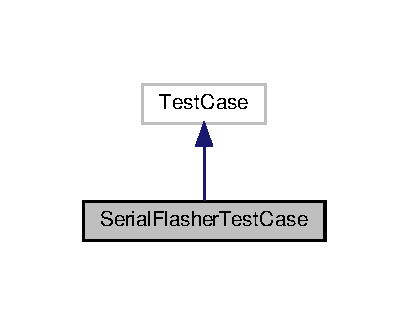
\includegraphics[width=196pt]{classstm__tools_1_1tests_1_1serialflasher__test_1_1SerialFlasherTestCase__inherit__graph}
\end{center}
\end{figure}


Collaboration diagram for Serial\+Flasher\+Test\+Case\+:
\nopagebreak
\begin{figure}[H]
\begin{center}
\leavevmode
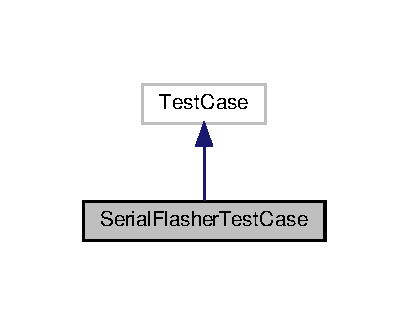
\includegraphics[width=196pt]{classstm__tools_1_1tests_1_1serialflasher__test_1_1SerialFlasherTestCase__coll__graph}
\end{center}
\end{figure}
\subsection*{Public Member Functions}
\begin{DoxyCompactItemize}
\item 
def \hyperlink{classstm__tools_1_1tests_1_1serialflasher__test_1_1SerialFlasherTestCase_a26b1b5aaa859d024cb7114cc1d4c1fd2}{set\+Up} (self)
\item 
def \hyperlink{classstm__tools_1_1tests_1_1serialflasher__test_1_1SerialFlasherTestCase_a56c54e463c817da67a20bb5e7b3b433a}{tear\+Down} (self)
\item 
def \hyperlink{classstm__tools_1_1tests_1_1serialflasher__test_1_1SerialFlasherTestCase_a3c64ad4ffc70313fb320cbff348ca340}{reset\+Device} (self)
\item 
def \hyperlink{classstm__tools_1_1tests_1_1serialflasher__test_1_1SerialFlasherTestCase_a6196826ae4218aa1d998d46082d63e32}{test\+Get\+Byte\+Complement} (self)
\item 
def \hyperlink{classstm__tools_1_1tests_1_1serialflasher__test_1_1SerialFlasherTestCase_ab3bae2350dc5fe3a1648fade1f3a220e}{test\+Append\+Checksum} (self)
\item 
def \hyperlink{classstm__tools_1_1tests_1_1serialflasher__test_1_1SerialFlasherTestCase_a7b9e64e2d4d21e7661b78b9be72fbc5c}{test\+Address\+To\+Bytes} (self)
\item 
def \hyperlink{classstm__tools_1_1tests_1_1serialflasher__test_1_1SerialFlasherTestCase_aa04254363060fbf88e9842fc5af0e984}{test\+Get\+Baud} (self)
\item 
def \hyperlink{classstm__tools_1_1tests_1_1serialflasher__test_1_1SerialFlasherTestCase_a09aac660829ca8fa8f1756fed0259dbf}{test\+Set\+Baud\+Valid} (self)
\item 
def \hyperlink{classstm__tools_1_1tests_1_1serialflasher__test_1_1SerialFlasherTestCase_aba049008f1b0bf098a9e9f385605f2b7}{test\+Set\+Baud\+Too\+Low} (self)
\item 
def \hyperlink{classstm__tools_1_1tests_1_1serialflasher__test_1_1SerialFlasherTestCase_a166cbd10369a00e75b9007161f8b4e2a}{test\+Set\+Baud\+Too\+High} (self)
\item 
def \hyperlink{classstm__tools_1_1tests_1_1serialflasher__test_1_1SerialFlasherTestCase_a5fb7594f713b3585700d0e388678e3be}{test\+Get\+Port} (self)
\item 
def \hyperlink{classstm__tools_1_1tests_1_1serialflasher__test_1_1SerialFlasherTestCase_a4c49f2b638d34ec72b059278a381ad51}{test\+Get\+Timeout} (self)
\item 
def \hyperlink{classstm__tools_1_1tests_1_1serialflasher__test_1_1SerialFlasherTestCase_ae3c687b584b4a279bd9df22cb2fef811}{test\+Set\+Serial\+Timeout} (self)
\item 
def \hyperlink{classstm__tools_1_1tests_1_1serialflasher__test_1_1SerialFlasherTestCase_a863c0a82485e80b7005e738b2bacefb8}{test\+Get\+Serial\+State} (self)
\item 
def \hyperlink{classstm__tools_1_1tests_1_1serialflasher__test_1_1SerialFlasherTestCase_a114db03b48126022cfcd2d0dc4fb26b3}{test\+Connect} (self)
\item 
def \hyperlink{classstm__tools_1_1tests_1_1serialflasher__test_1_1SerialFlasherTestCase_ac1cbca85ce618094d632a0af16ba52e6}{test\+Connected\+State} (self)
\item 
def \hyperlink{classstm__tools_1_1tests_1_1serialflasher__test_1_1SerialFlasherTestCase_ac9751871872b8bfb27e061c108222282}{test\+Disconnect} (self)
\item 
def \hyperlink{classstm__tools_1_1tests_1_1serialflasher__test_1_1SerialFlasherTestCase_af486717823faa844b9bc5d9cb03f7b61}{test\+Set\+Baud\+Whilst\+Connected} (self)
\item 
def \hyperlink{classstm__tools_1_1tests_1_1serialflasher__test_1_1SerialFlasherTestCase_a103102126afd6a4b959d0c10473cc787}{test\+Cmd\+Get\+Id} (self)
\item 
def \hyperlink{classstm__tools_1_1tests_1_1serialflasher__test_1_1SerialFlasherTestCase_a8c6d66f97f8060adc810eb666ef4cca7}{test\+Cmd\+Get\+Version\+Prot} (self)
\item 
def \hyperlink{classstm__tools_1_1tests_1_1serialflasher__test_1_1SerialFlasherTestCase_abcb99be50edb3c671a3b2a8246921600}{test\+Read\+Memory\+Address} (self)
\item 
def \hyperlink{classstm__tools_1_1tests_1_1serialflasher__test_1_1SerialFlasherTestCase_a5b970a4209778cf5951059570a5fad06}{test\+Read\+Ram\+Memory\+Address} (self)
\item 
def \hyperlink{classstm__tools_1_1tests_1_1serialflasher__test_1_1SerialFlasherTestCase_a000717609bc7fcbdcd0466f55c6593d6}{test\+Cmd\+Write\+Memory\+Address\+Ram} (self)
\item 
def \hyperlink{classstm__tools_1_1tests_1_1serialflasher__test_1_1SerialFlasherTestCase_af6c1e00106ebeaf5cdaf948b299f988a}{test\+Cmd\+Write\+Memory\+Address\+Protected} (self)
\item 
def \hyperlink{classstm__tools_1_1tests_1_1serialflasher__test_1_1SerialFlasherTestCase_a61f04287c66a27d3a90210980b991b55}{test\+Cmd\+Write\+Read\+Memory\+Address\+Ram} (self)
\item 
def \hyperlink{classstm__tools_1_1tests_1_1serialflasher__test_1_1SerialFlasherTestCase_aeadcb812deb6d74af00e557b59bb3906}{test\+Cmd\+Write\+Protect} (self)
\item 
def \hyperlink{classstm__tools_1_1tests_1_1serialflasher__test_1_1SerialFlasherTestCase_ac137024da2dc3ada51d8cb8bc1d4eca9}{test\+Cmd\+Write\+Unprotect} (self)
\item 
def \hyperlink{classstm__tools_1_1tests_1_1serialflasher__test_1_1SerialFlasherTestCase_a643113c69f00e161c618ba8a8e0c894a}{test\+Cmd\+Read\+Protect} (self)
\item 
def \hyperlink{classstm__tools_1_1tests_1_1serialflasher__test_1_1SerialFlasherTestCase_a3b8dd28cc2525171c4cd37e5d212a005}{test\+Cmd\+Read\+Unprotect} (self)
\end{DoxyCompactItemize}
\subsection*{Public Attributes}
\begin{DoxyCompactItemize}
\item 
\hyperlink{classstm__tools_1_1tests_1_1serialflasher__test_1_1SerialFlasherTestCase_afae8c8266de12daf134ef2bf3a869f65}{serial}
\item 
\hyperlink{classstm__tools_1_1tests_1_1serialflasher__test_1_1SerialFlasherTestCase_ad713e38281718ed2d493fdcfa44dac7e}{sf}
\end{DoxyCompactItemize}


\subsection{Member Function Documentation}
\mbox{\Hypertarget{classstm__tools_1_1tests_1_1serialflasher__test_1_1SerialFlasherTestCase_a3c64ad4ffc70313fb320cbff348ca340}\label{classstm__tools_1_1tests_1_1serialflasher__test_1_1SerialFlasherTestCase_a3c64ad4ffc70313fb320cbff348ca340}} 
\index{stm\+\_\+tools\+::tests\+::serialflasher\+\_\+test\+::\+Serial\+Flasher\+Test\+Case@{stm\+\_\+tools\+::tests\+::serialflasher\+\_\+test\+::\+Serial\+Flasher\+Test\+Case}!reset\+Device@{reset\+Device}}
\index{reset\+Device@{reset\+Device}!stm\+\_\+tools\+::tests\+::serialflasher\+\_\+test\+::\+Serial\+Flasher\+Test\+Case@{stm\+\_\+tools\+::tests\+::serialflasher\+\_\+test\+::\+Serial\+Flasher\+Test\+Case}}
\subsubsection{\texorpdfstring{reset\+Device()}{resetDevice()}}
{\footnotesize\ttfamily def reset\+Device (\begin{DoxyParamCaption}\item[{}]{self }\end{DoxyParamCaption})}

\begin{DoxyVerb}uses the DTR pin of USB->Serial to reset board\end{DoxyVerb}
 \mbox{\Hypertarget{classstm__tools_1_1tests_1_1serialflasher__test_1_1SerialFlasherTestCase_a26b1b5aaa859d024cb7114cc1d4c1fd2}\label{classstm__tools_1_1tests_1_1serialflasher__test_1_1SerialFlasherTestCase_a26b1b5aaa859d024cb7114cc1d4c1fd2}} 
\index{stm\+\_\+tools\+::tests\+::serialflasher\+\_\+test\+::\+Serial\+Flasher\+Test\+Case@{stm\+\_\+tools\+::tests\+::serialflasher\+\_\+test\+::\+Serial\+Flasher\+Test\+Case}!set\+Up@{set\+Up}}
\index{set\+Up@{set\+Up}!stm\+\_\+tools\+::tests\+::serialflasher\+\_\+test\+::\+Serial\+Flasher\+Test\+Case@{stm\+\_\+tools\+::tests\+::serialflasher\+\_\+test\+::\+Serial\+Flasher\+Test\+Case}}
\subsubsection{\texorpdfstring{set\+Up()}{setUp()}}
{\footnotesize\ttfamily def set\+Up (\begin{DoxyParamCaption}\item[{}]{self }\end{DoxyParamCaption})}

\mbox{\Hypertarget{classstm__tools_1_1tests_1_1serialflasher__test_1_1SerialFlasherTestCase_a56c54e463c817da67a20bb5e7b3b433a}\label{classstm__tools_1_1tests_1_1serialflasher__test_1_1SerialFlasherTestCase_a56c54e463c817da67a20bb5e7b3b433a}} 
\index{stm\+\_\+tools\+::tests\+::serialflasher\+\_\+test\+::\+Serial\+Flasher\+Test\+Case@{stm\+\_\+tools\+::tests\+::serialflasher\+\_\+test\+::\+Serial\+Flasher\+Test\+Case}!tear\+Down@{tear\+Down}}
\index{tear\+Down@{tear\+Down}!stm\+\_\+tools\+::tests\+::serialflasher\+\_\+test\+::\+Serial\+Flasher\+Test\+Case@{stm\+\_\+tools\+::tests\+::serialflasher\+\_\+test\+::\+Serial\+Flasher\+Test\+Case}}
\subsubsection{\texorpdfstring{tear\+Down()}{tearDown()}}
{\footnotesize\ttfamily def tear\+Down (\begin{DoxyParamCaption}\item[{}]{self }\end{DoxyParamCaption})}

\begin{DoxyVerb}Teardown: Close socket and reset device\end{DoxyVerb}
 \mbox{\Hypertarget{classstm__tools_1_1tests_1_1serialflasher__test_1_1SerialFlasherTestCase_a7b9e64e2d4d21e7661b78b9be72fbc5c}\label{classstm__tools_1_1tests_1_1serialflasher__test_1_1SerialFlasherTestCase_a7b9e64e2d4d21e7661b78b9be72fbc5c}} 
\index{stm\+\_\+tools\+::tests\+::serialflasher\+\_\+test\+::\+Serial\+Flasher\+Test\+Case@{stm\+\_\+tools\+::tests\+::serialflasher\+\_\+test\+::\+Serial\+Flasher\+Test\+Case}!test\+Address\+To\+Bytes@{test\+Address\+To\+Bytes}}
\index{test\+Address\+To\+Bytes@{test\+Address\+To\+Bytes}!stm\+\_\+tools\+::tests\+::serialflasher\+\_\+test\+::\+Serial\+Flasher\+Test\+Case@{stm\+\_\+tools\+::tests\+::serialflasher\+\_\+test\+::\+Serial\+Flasher\+Test\+Case}}
\subsubsection{\texorpdfstring{test\+Address\+To\+Bytes()}{testAddressToBytes()}}
{\footnotesize\ttfamily def test\+Address\+To\+Bytes (\begin{DoxyParamCaption}\item[{}]{self }\end{DoxyParamCaption})}

\mbox{\Hypertarget{classstm__tools_1_1tests_1_1serialflasher__test_1_1SerialFlasherTestCase_ab3bae2350dc5fe3a1648fade1f3a220e}\label{classstm__tools_1_1tests_1_1serialflasher__test_1_1SerialFlasherTestCase_ab3bae2350dc5fe3a1648fade1f3a220e}} 
\index{stm\+\_\+tools\+::tests\+::serialflasher\+\_\+test\+::\+Serial\+Flasher\+Test\+Case@{stm\+\_\+tools\+::tests\+::serialflasher\+\_\+test\+::\+Serial\+Flasher\+Test\+Case}!test\+Append\+Checksum@{test\+Append\+Checksum}}
\index{test\+Append\+Checksum@{test\+Append\+Checksum}!stm\+\_\+tools\+::tests\+::serialflasher\+\_\+test\+::\+Serial\+Flasher\+Test\+Case@{stm\+\_\+tools\+::tests\+::serialflasher\+\_\+test\+::\+Serial\+Flasher\+Test\+Case}}
\subsubsection{\texorpdfstring{test\+Append\+Checksum()}{testAppendChecksum()}}
{\footnotesize\ttfamily def test\+Append\+Checksum (\begin{DoxyParamCaption}\item[{}]{self }\end{DoxyParamCaption})}

\mbox{\Hypertarget{classstm__tools_1_1tests_1_1serialflasher__test_1_1SerialFlasherTestCase_a103102126afd6a4b959d0c10473cc787}\label{classstm__tools_1_1tests_1_1serialflasher__test_1_1SerialFlasherTestCase_a103102126afd6a4b959d0c10473cc787}} 
\index{stm\+\_\+tools\+::tests\+::serialflasher\+\_\+test\+::\+Serial\+Flasher\+Test\+Case@{stm\+\_\+tools\+::tests\+::serialflasher\+\_\+test\+::\+Serial\+Flasher\+Test\+Case}!test\+Cmd\+Get\+Id@{test\+Cmd\+Get\+Id}}
\index{test\+Cmd\+Get\+Id@{test\+Cmd\+Get\+Id}!stm\+\_\+tools\+::tests\+::serialflasher\+\_\+test\+::\+Serial\+Flasher\+Test\+Case@{stm\+\_\+tools\+::tests\+::serialflasher\+\_\+test\+::\+Serial\+Flasher\+Test\+Case}}
\subsubsection{\texorpdfstring{test\+Cmd\+Get\+Id()}{testCmdGetId()}}
{\footnotesize\ttfamily def test\+Cmd\+Get\+Id (\begin{DoxyParamCaption}\item[{}]{self }\end{DoxyParamCaption})}

\begin{DoxyVerb}test we can get the device id\end{DoxyVerb}
 \mbox{\Hypertarget{classstm__tools_1_1tests_1_1serialflasher__test_1_1SerialFlasherTestCase_a8c6d66f97f8060adc810eb666ef4cca7}\label{classstm__tools_1_1tests_1_1serialflasher__test_1_1SerialFlasherTestCase_a8c6d66f97f8060adc810eb666ef4cca7}} 
\index{stm\+\_\+tools\+::tests\+::serialflasher\+\_\+test\+::\+Serial\+Flasher\+Test\+Case@{stm\+\_\+tools\+::tests\+::serialflasher\+\_\+test\+::\+Serial\+Flasher\+Test\+Case}!test\+Cmd\+Get\+Version\+Prot@{test\+Cmd\+Get\+Version\+Prot}}
\index{test\+Cmd\+Get\+Version\+Prot@{test\+Cmd\+Get\+Version\+Prot}!stm\+\_\+tools\+::tests\+::serialflasher\+\_\+test\+::\+Serial\+Flasher\+Test\+Case@{stm\+\_\+tools\+::tests\+::serialflasher\+\_\+test\+::\+Serial\+Flasher\+Test\+Case}}
\subsubsection{\texorpdfstring{test\+Cmd\+Get\+Version\+Prot()}{testCmdGetVersionProt()}}
{\footnotesize\ttfamily def test\+Cmd\+Get\+Version\+Prot (\begin{DoxyParamCaption}\item[{}]{self }\end{DoxyParamCaption})}

\begin{DoxyVerb}interested to see what these other commands return
and compare to the GET command output
\end{DoxyVerb}
 \mbox{\Hypertarget{classstm__tools_1_1tests_1_1serialflasher__test_1_1SerialFlasherTestCase_a643113c69f00e161c618ba8a8e0c894a}\label{classstm__tools_1_1tests_1_1serialflasher__test_1_1SerialFlasherTestCase_a643113c69f00e161c618ba8a8e0c894a}} 
\index{stm\+\_\+tools\+::tests\+::serialflasher\+\_\+test\+::\+Serial\+Flasher\+Test\+Case@{stm\+\_\+tools\+::tests\+::serialflasher\+\_\+test\+::\+Serial\+Flasher\+Test\+Case}!test\+Cmd\+Read\+Protect@{test\+Cmd\+Read\+Protect}}
\index{test\+Cmd\+Read\+Protect@{test\+Cmd\+Read\+Protect}!stm\+\_\+tools\+::tests\+::serialflasher\+\_\+test\+::\+Serial\+Flasher\+Test\+Case@{stm\+\_\+tools\+::tests\+::serialflasher\+\_\+test\+::\+Serial\+Flasher\+Test\+Case}}
\subsubsection{\texorpdfstring{test\+Cmd\+Read\+Protect()}{testCmdReadProtect()}}
{\footnotesize\ttfamily def test\+Cmd\+Read\+Protect (\begin{DoxyParamCaption}\item[{}]{self }\end{DoxyParamCaption})}

\mbox{\Hypertarget{classstm__tools_1_1tests_1_1serialflasher__test_1_1SerialFlasherTestCase_a3b8dd28cc2525171c4cd37e5d212a005}\label{classstm__tools_1_1tests_1_1serialflasher__test_1_1SerialFlasherTestCase_a3b8dd28cc2525171c4cd37e5d212a005}} 
\index{stm\+\_\+tools\+::tests\+::serialflasher\+\_\+test\+::\+Serial\+Flasher\+Test\+Case@{stm\+\_\+tools\+::tests\+::serialflasher\+\_\+test\+::\+Serial\+Flasher\+Test\+Case}!test\+Cmd\+Read\+Unprotect@{test\+Cmd\+Read\+Unprotect}}
\index{test\+Cmd\+Read\+Unprotect@{test\+Cmd\+Read\+Unprotect}!stm\+\_\+tools\+::tests\+::serialflasher\+\_\+test\+::\+Serial\+Flasher\+Test\+Case@{stm\+\_\+tools\+::tests\+::serialflasher\+\_\+test\+::\+Serial\+Flasher\+Test\+Case}}
\subsubsection{\texorpdfstring{test\+Cmd\+Read\+Unprotect()}{testCmdReadUnprotect()}}
{\footnotesize\ttfamily def test\+Cmd\+Read\+Unprotect (\begin{DoxyParamCaption}\item[{}]{self }\end{DoxyParamCaption})}

\mbox{\Hypertarget{classstm__tools_1_1tests_1_1serialflasher__test_1_1SerialFlasherTestCase_af6c1e00106ebeaf5cdaf948b299f988a}\label{classstm__tools_1_1tests_1_1serialflasher__test_1_1SerialFlasherTestCase_af6c1e00106ebeaf5cdaf948b299f988a}} 
\index{stm\+\_\+tools\+::tests\+::serialflasher\+\_\+test\+::\+Serial\+Flasher\+Test\+Case@{stm\+\_\+tools\+::tests\+::serialflasher\+\_\+test\+::\+Serial\+Flasher\+Test\+Case}!test\+Cmd\+Write\+Memory\+Address\+Protected@{test\+Cmd\+Write\+Memory\+Address\+Protected}}
\index{test\+Cmd\+Write\+Memory\+Address\+Protected@{test\+Cmd\+Write\+Memory\+Address\+Protected}!stm\+\_\+tools\+::tests\+::serialflasher\+\_\+test\+::\+Serial\+Flasher\+Test\+Case@{stm\+\_\+tools\+::tests\+::serialflasher\+\_\+test\+::\+Serial\+Flasher\+Test\+Case}}
\subsubsection{\texorpdfstring{test\+Cmd\+Write\+Memory\+Address\+Protected()}{testCmdWriteMemoryAddressProtected()}}
{\footnotesize\ttfamily def test\+Cmd\+Write\+Memory\+Address\+Protected (\begin{DoxyParamCaption}\item[{}]{self }\end{DoxyParamCaption})}

\mbox{\Hypertarget{classstm__tools_1_1tests_1_1serialflasher__test_1_1SerialFlasherTestCase_a000717609bc7fcbdcd0466f55c6593d6}\label{classstm__tools_1_1tests_1_1serialflasher__test_1_1SerialFlasherTestCase_a000717609bc7fcbdcd0466f55c6593d6}} 
\index{stm\+\_\+tools\+::tests\+::serialflasher\+\_\+test\+::\+Serial\+Flasher\+Test\+Case@{stm\+\_\+tools\+::tests\+::serialflasher\+\_\+test\+::\+Serial\+Flasher\+Test\+Case}!test\+Cmd\+Write\+Memory\+Address\+Ram@{test\+Cmd\+Write\+Memory\+Address\+Ram}}
\index{test\+Cmd\+Write\+Memory\+Address\+Ram@{test\+Cmd\+Write\+Memory\+Address\+Ram}!stm\+\_\+tools\+::tests\+::serialflasher\+\_\+test\+::\+Serial\+Flasher\+Test\+Case@{stm\+\_\+tools\+::tests\+::serialflasher\+\_\+test\+::\+Serial\+Flasher\+Test\+Case}}
\subsubsection{\texorpdfstring{test\+Cmd\+Write\+Memory\+Address\+Ram()}{testCmdWriteMemoryAddressRam()}}
{\footnotesize\ttfamily def test\+Cmd\+Write\+Memory\+Address\+Ram (\begin{DoxyParamCaption}\item[{}]{self }\end{DoxyParamCaption})}

\mbox{\Hypertarget{classstm__tools_1_1tests_1_1serialflasher__test_1_1SerialFlasherTestCase_aeadcb812deb6d74af00e557b59bb3906}\label{classstm__tools_1_1tests_1_1serialflasher__test_1_1SerialFlasherTestCase_aeadcb812deb6d74af00e557b59bb3906}} 
\index{stm\+\_\+tools\+::tests\+::serialflasher\+\_\+test\+::\+Serial\+Flasher\+Test\+Case@{stm\+\_\+tools\+::tests\+::serialflasher\+\_\+test\+::\+Serial\+Flasher\+Test\+Case}!test\+Cmd\+Write\+Protect@{test\+Cmd\+Write\+Protect}}
\index{test\+Cmd\+Write\+Protect@{test\+Cmd\+Write\+Protect}!stm\+\_\+tools\+::tests\+::serialflasher\+\_\+test\+::\+Serial\+Flasher\+Test\+Case@{stm\+\_\+tools\+::tests\+::serialflasher\+\_\+test\+::\+Serial\+Flasher\+Test\+Case}}
\subsubsection{\texorpdfstring{test\+Cmd\+Write\+Protect()}{testCmdWriteProtect()}}
{\footnotesize\ttfamily def test\+Cmd\+Write\+Protect (\begin{DoxyParamCaption}\item[{}]{self }\end{DoxyParamCaption})}

\begin{DoxyVerb}test command write protect succeeds -
TODO: should check the
     the option bytes to confirm
\end{DoxyVerb}
 \mbox{\Hypertarget{classstm__tools_1_1tests_1_1serialflasher__test_1_1SerialFlasherTestCase_a61f04287c66a27d3a90210980b991b55}\label{classstm__tools_1_1tests_1_1serialflasher__test_1_1SerialFlasherTestCase_a61f04287c66a27d3a90210980b991b55}} 
\index{stm\+\_\+tools\+::tests\+::serialflasher\+\_\+test\+::\+Serial\+Flasher\+Test\+Case@{stm\+\_\+tools\+::tests\+::serialflasher\+\_\+test\+::\+Serial\+Flasher\+Test\+Case}!test\+Cmd\+Write\+Read\+Memory\+Address\+Ram@{test\+Cmd\+Write\+Read\+Memory\+Address\+Ram}}
\index{test\+Cmd\+Write\+Read\+Memory\+Address\+Ram@{test\+Cmd\+Write\+Read\+Memory\+Address\+Ram}!stm\+\_\+tools\+::tests\+::serialflasher\+\_\+test\+::\+Serial\+Flasher\+Test\+Case@{stm\+\_\+tools\+::tests\+::serialflasher\+\_\+test\+::\+Serial\+Flasher\+Test\+Case}}
\subsubsection{\texorpdfstring{test\+Cmd\+Write\+Read\+Memory\+Address\+Ram()}{testCmdWriteReadMemoryAddressRam()}}
{\footnotesize\ttfamily def test\+Cmd\+Write\+Read\+Memory\+Address\+Ram (\begin{DoxyParamCaption}\item[{}]{self }\end{DoxyParamCaption})}

\mbox{\Hypertarget{classstm__tools_1_1tests_1_1serialflasher__test_1_1SerialFlasherTestCase_ac137024da2dc3ada51d8cb8bc1d4eca9}\label{classstm__tools_1_1tests_1_1serialflasher__test_1_1SerialFlasherTestCase_ac137024da2dc3ada51d8cb8bc1d4eca9}} 
\index{stm\+\_\+tools\+::tests\+::serialflasher\+\_\+test\+::\+Serial\+Flasher\+Test\+Case@{stm\+\_\+tools\+::tests\+::serialflasher\+\_\+test\+::\+Serial\+Flasher\+Test\+Case}!test\+Cmd\+Write\+Unprotect@{test\+Cmd\+Write\+Unprotect}}
\index{test\+Cmd\+Write\+Unprotect@{test\+Cmd\+Write\+Unprotect}!stm\+\_\+tools\+::tests\+::serialflasher\+\_\+test\+::\+Serial\+Flasher\+Test\+Case@{stm\+\_\+tools\+::tests\+::serialflasher\+\_\+test\+::\+Serial\+Flasher\+Test\+Case}}
\subsubsection{\texorpdfstring{test\+Cmd\+Write\+Unprotect()}{testCmdWriteUnprotect()}}
{\footnotesize\ttfamily def test\+Cmd\+Write\+Unprotect (\begin{DoxyParamCaption}\item[{}]{self }\end{DoxyParamCaption})}

\mbox{\Hypertarget{classstm__tools_1_1tests_1_1serialflasher__test_1_1SerialFlasherTestCase_a114db03b48126022cfcd2d0dc4fb26b3}\label{classstm__tools_1_1tests_1_1serialflasher__test_1_1SerialFlasherTestCase_a114db03b48126022cfcd2d0dc4fb26b3}} 
\index{stm\+\_\+tools\+::tests\+::serialflasher\+\_\+test\+::\+Serial\+Flasher\+Test\+Case@{stm\+\_\+tools\+::tests\+::serialflasher\+\_\+test\+::\+Serial\+Flasher\+Test\+Case}!test\+Connect@{test\+Connect}}
\index{test\+Connect@{test\+Connect}!stm\+\_\+tools\+::tests\+::serialflasher\+\_\+test\+::\+Serial\+Flasher\+Test\+Case@{stm\+\_\+tools\+::tests\+::serialflasher\+\_\+test\+::\+Serial\+Flasher\+Test\+Case}}
\subsubsection{\texorpdfstring{test\+Connect()}{testConnect()}}
{\footnotesize\ttfamily def test\+Connect (\begin{DoxyParamCaption}\item[{}]{self }\end{DoxyParamCaption})}

\begin{DoxyVerb}test we can connect to the device\end{DoxyVerb}
 \mbox{\Hypertarget{classstm__tools_1_1tests_1_1serialflasher__test_1_1SerialFlasherTestCase_ac1cbca85ce618094d632a0af16ba52e6}\label{classstm__tools_1_1tests_1_1serialflasher__test_1_1SerialFlasherTestCase_ac1cbca85ce618094d632a0af16ba52e6}} 
\index{stm\+\_\+tools\+::tests\+::serialflasher\+\_\+test\+::\+Serial\+Flasher\+Test\+Case@{stm\+\_\+tools\+::tests\+::serialflasher\+\_\+test\+::\+Serial\+Flasher\+Test\+Case}!test\+Connected\+State@{test\+Connected\+State}}
\index{test\+Connected\+State@{test\+Connected\+State}!stm\+\_\+tools\+::tests\+::serialflasher\+\_\+test\+::\+Serial\+Flasher\+Test\+Case@{stm\+\_\+tools\+::tests\+::serialflasher\+\_\+test\+::\+Serial\+Flasher\+Test\+Case}}
\subsubsection{\texorpdfstring{test\+Connected\+State()}{testConnectedState()}}
{\footnotesize\ttfamily def test\+Connected\+State (\begin{DoxyParamCaption}\item[{}]{self }\end{DoxyParamCaption})}

\mbox{\Hypertarget{classstm__tools_1_1tests_1_1serialflasher__test_1_1SerialFlasherTestCase_ac9751871872b8bfb27e061c108222282}\label{classstm__tools_1_1tests_1_1serialflasher__test_1_1SerialFlasherTestCase_ac9751871872b8bfb27e061c108222282}} 
\index{stm\+\_\+tools\+::tests\+::serialflasher\+\_\+test\+::\+Serial\+Flasher\+Test\+Case@{stm\+\_\+tools\+::tests\+::serialflasher\+\_\+test\+::\+Serial\+Flasher\+Test\+Case}!test\+Disconnect@{test\+Disconnect}}
\index{test\+Disconnect@{test\+Disconnect}!stm\+\_\+tools\+::tests\+::serialflasher\+\_\+test\+::\+Serial\+Flasher\+Test\+Case@{stm\+\_\+tools\+::tests\+::serialflasher\+\_\+test\+::\+Serial\+Flasher\+Test\+Case}}
\subsubsection{\texorpdfstring{test\+Disconnect()}{testDisconnect()}}
{\footnotesize\ttfamily def test\+Disconnect (\begin{DoxyParamCaption}\item[{}]{self }\end{DoxyParamCaption})}

\begin{DoxyVerb}test we can disconnect from the device and close the serial port\end{DoxyVerb}
 \mbox{\Hypertarget{classstm__tools_1_1tests_1_1serialflasher__test_1_1SerialFlasherTestCase_aa04254363060fbf88e9842fc5af0e984}\label{classstm__tools_1_1tests_1_1serialflasher__test_1_1SerialFlasherTestCase_aa04254363060fbf88e9842fc5af0e984}} 
\index{stm\+\_\+tools\+::tests\+::serialflasher\+\_\+test\+::\+Serial\+Flasher\+Test\+Case@{stm\+\_\+tools\+::tests\+::serialflasher\+\_\+test\+::\+Serial\+Flasher\+Test\+Case}!test\+Get\+Baud@{test\+Get\+Baud}}
\index{test\+Get\+Baud@{test\+Get\+Baud}!stm\+\_\+tools\+::tests\+::serialflasher\+\_\+test\+::\+Serial\+Flasher\+Test\+Case@{stm\+\_\+tools\+::tests\+::serialflasher\+\_\+test\+::\+Serial\+Flasher\+Test\+Case}}
\subsubsection{\texorpdfstring{test\+Get\+Baud()}{testGetBaud()}}
{\footnotesize\ttfamily def test\+Get\+Baud (\begin{DoxyParamCaption}\item[{}]{self }\end{DoxyParamCaption})}

\begin{DoxyVerb}test we can get the baud property\end{DoxyVerb}
 \mbox{\Hypertarget{classstm__tools_1_1tests_1_1serialflasher__test_1_1SerialFlasherTestCase_a6196826ae4218aa1d998d46082d63e32}\label{classstm__tools_1_1tests_1_1serialflasher__test_1_1SerialFlasherTestCase_a6196826ae4218aa1d998d46082d63e32}} 
\index{stm\+\_\+tools\+::tests\+::serialflasher\+\_\+test\+::\+Serial\+Flasher\+Test\+Case@{stm\+\_\+tools\+::tests\+::serialflasher\+\_\+test\+::\+Serial\+Flasher\+Test\+Case}!test\+Get\+Byte\+Complement@{test\+Get\+Byte\+Complement}}
\index{test\+Get\+Byte\+Complement@{test\+Get\+Byte\+Complement}!stm\+\_\+tools\+::tests\+::serialflasher\+\_\+test\+::\+Serial\+Flasher\+Test\+Case@{stm\+\_\+tools\+::tests\+::serialflasher\+\_\+test\+::\+Serial\+Flasher\+Test\+Case}}
\subsubsection{\texorpdfstring{test\+Get\+Byte\+Complement()}{testGetByteComplement()}}
{\footnotesize\ttfamily def test\+Get\+Byte\+Complement (\begin{DoxyParamCaption}\item[{}]{self }\end{DoxyParamCaption})}

\mbox{\Hypertarget{classstm__tools_1_1tests_1_1serialflasher__test_1_1SerialFlasherTestCase_a5fb7594f713b3585700d0e388678e3be}\label{classstm__tools_1_1tests_1_1serialflasher__test_1_1SerialFlasherTestCase_a5fb7594f713b3585700d0e388678e3be}} 
\index{stm\+\_\+tools\+::tests\+::serialflasher\+\_\+test\+::\+Serial\+Flasher\+Test\+Case@{stm\+\_\+tools\+::tests\+::serialflasher\+\_\+test\+::\+Serial\+Flasher\+Test\+Case}!test\+Get\+Port@{test\+Get\+Port}}
\index{test\+Get\+Port@{test\+Get\+Port}!stm\+\_\+tools\+::tests\+::serialflasher\+\_\+test\+::\+Serial\+Flasher\+Test\+Case@{stm\+\_\+tools\+::tests\+::serialflasher\+\_\+test\+::\+Serial\+Flasher\+Test\+Case}}
\subsubsection{\texorpdfstring{test\+Get\+Port()}{testGetPort()}}
{\footnotesize\ttfamily def test\+Get\+Port (\begin{DoxyParamCaption}\item[{}]{self }\end{DoxyParamCaption})}

\begin{DoxyVerb}test we can get the connected port\end{DoxyVerb}
 \mbox{\Hypertarget{classstm__tools_1_1tests_1_1serialflasher__test_1_1SerialFlasherTestCase_a863c0a82485e80b7005e738b2bacefb8}\label{classstm__tools_1_1tests_1_1serialflasher__test_1_1SerialFlasherTestCase_a863c0a82485e80b7005e738b2bacefb8}} 
\index{stm\+\_\+tools\+::tests\+::serialflasher\+\_\+test\+::\+Serial\+Flasher\+Test\+Case@{stm\+\_\+tools\+::tests\+::serialflasher\+\_\+test\+::\+Serial\+Flasher\+Test\+Case}!test\+Get\+Serial\+State@{test\+Get\+Serial\+State}}
\index{test\+Get\+Serial\+State@{test\+Get\+Serial\+State}!stm\+\_\+tools\+::tests\+::serialflasher\+\_\+test\+::\+Serial\+Flasher\+Test\+Case@{stm\+\_\+tools\+::tests\+::serialflasher\+\_\+test\+::\+Serial\+Flasher\+Test\+Case}}
\subsubsection{\texorpdfstring{test\+Get\+Serial\+State()}{testGetSerialState()}}
{\footnotesize\ttfamily def test\+Get\+Serial\+State (\begin{DoxyParamCaption}\item[{}]{self }\end{DoxyParamCaption})}

\begin{DoxyVerb}test we can get the serial state\end{DoxyVerb}
 \mbox{\Hypertarget{classstm__tools_1_1tests_1_1serialflasher__test_1_1SerialFlasherTestCase_a4c49f2b638d34ec72b059278a381ad51}\label{classstm__tools_1_1tests_1_1serialflasher__test_1_1SerialFlasherTestCase_a4c49f2b638d34ec72b059278a381ad51}} 
\index{stm\+\_\+tools\+::tests\+::serialflasher\+\_\+test\+::\+Serial\+Flasher\+Test\+Case@{stm\+\_\+tools\+::tests\+::serialflasher\+\_\+test\+::\+Serial\+Flasher\+Test\+Case}!test\+Get\+Timeout@{test\+Get\+Timeout}}
\index{test\+Get\+Timeout@{test\+Get\+Timeout}!stm\+\_\+tools\+::tests\+::serialflasher\+\_\+test\+::\+Serial\+Flasher\+Test\+Case@{stm\+\_\+tools\+::tests\+::serialflasher\+\_\+test\+::\+Serial\+Flasher\+Test\+Case}}
\subsubsection{\texorpdfstring{test\+Get\+Timeout()}{testGetTimeout()}}
{\footnotesize\ttfamily def test\+Get\+Timeout (\begin{DoxyParamCaption}\item[{}]{self }\end{DoxyParamCaption})}

\begin{DoxyVerb}test we can get the serial timeout\end{DoxyVerb}
 \mbox{\Hypertarget{classstm__tools_1_1tests_1_1serialflasher__test_1_1SerialFlasherTestCase_abcb99be50edb3c671a3b2a8246921600}\label{classstm__tools_1_1tests_1_1serialflasher__test_1_1SerialFlasherTestCase_abcb99be50edb3c671a3b2a8246921600}} 
\index{stm\+\_\+tools\+::tests\+::serialflasher\+\_\+test\+::\+Serial\+Flasher\+Test\+Case@{stm\+\_\+tools\+::tests\+::serialflasher\+\_\+test\+::\+Serial\+Flasher\+Test\+Case}!test\+Read\+Memory\+Address@{test\+Read\+Memory\+Address}}
\index{test\+Read\+Memory\+Address@{test\+Read\+Memory\+Address}!stm\+\_\+tools\+::tests\+::serialflasher\+\_\+test\+::\+Serial\+Flasher\+Test\+Case@{stm\+\_\+tools\+::tests\+::serialflasher\+\_\+test\+::\+Serial\+Flasher\+Test\+Case}}
\subsubsection{\texorpdfstring{test\+Read\+Memory\+Address()}{testReadMemoryAddress()}}
{\footnotesize\ttfamily def test\+Read\+Memory\+Address (\begin{DoxyParamCaption}\item[{}]{self }\end{DoxyParamCaption})}

\begin{DoxyVerb}test we can read from a known memory address
read a known fixed value from the device...
let's go look at the data sheet...
option byte seems a good target
also the flash CR - needs unlocked
\end{DoxyVerb}
 \mbox{\Hypertarget{classstm__tools_1_1tests_1_1serialflasher__test_1_1SerialFlasherTestCase_a5b970a4209778cf5951059570a5fad06}\label{classstm__tools_1_1tests_1_1serialflasher__test_1_1SerialFlasherTestCase_a5b970a4209778cf5951059570a5fad06}} 
\index{stm\+\_\+tools\+::tests\+::serialflasher\+\_\+test\+::\+Serial\+Flasher\+Test\+Case@{stm\+\_\+tools\+::tests\+::serialflasher\+\_\+test\+::\+Serial\+Flasher\+Test\+Case}!test\+Read\+Ram\+Memory\+Address@{test\+Read\+Ram\+Memory\+Address}}
\index{test\+Read\+Ram\+Memory\+Address@{test\+Read\+Ram\+Memory\+Address}!stm\+\_\+tools\+::tests\+::serialflasher\+\_\+test\+::\+Serial\+Flasher\+Test\+Case@{stm\+\_\+tools\+::tests\+::serialflasher\+\_\+test\+::\+Serial\+Flasher\+Test\+Case}}
\subsubsection{\texorpdfstring{test\+Read\+Ram\+Memory\+Address()}{testReadRamMemoryAddress()}}
{\footnotesize\ttfamily def test\+Read\+Ram\+Memory\+Address (\begin{DoxyParamCaption}\item[{}]{self }\end{DoxyParamCaption})}

\begin{DoxyVerb}test we can read from a ram address\end{DoxyVerb}
 \mbox{\Hypertarget{classstm__tools_1_1tests_1_1serialflasher__test_1_1SerialFlasherTestCase_a166cbd10369a00e75b9007161f8b4e2a}\label{classstm__tools_1_1tests_1_1serialflasher__test_1_1SerialFlasherTestCase_a166cbd10369a00e75b9007161f8b4e2a}} 
\index{stm\+\_\+tools\+::tests\+::serialflasher\+\_\+test\+::\+Serial\+Flasher\+Test\+Case@{stm\+\_\+tools\+::tests\+::serialflasher\+\_\+test\+::\+Serial\+Flasher\+Test\+Case}!test\+Set\+Baud\+Too\+High@{test\+Set\+Baud\+Too\+High}}
\index{test\+Set\+Baud\+Too\+High@{test\+Set\+Baud\+Too\+High}!stm\+\_\+tools\+::tests\+::serialflasher\+\_\+test\+::\+Serial\+Flasher\+Test\+Case@{stm\+\_\+tools\+::tests\+::serialflasher\+\_\+test\+::\+Serial\+Flasher\+Test\+Case}}
\subsubsection{\texorpdfstring{test\+Set\+Baud\+Too\+High()}{testSetBaudTooHigh()}}
{\footnotesize\ttfamily def test\+Set\+Baud\+Too\+High (\begin{DoxyParamCaption}\item[{}]{self }\end{DoxyParamCaption})}

\begin{DoxyVerb}test setting baud above max raises value error\end{DoxyVerb}
 \mbox{\Hypertarget{classstm__tools_1_1tests_1_1serialflasher__test_1_1SerialFlasherTestCase_aba049008f1b0bf098a9e9f385605f2b7}\label{classstm__tools_1_1tests_1_1serialflasher__test_1_1SerialFlasherTestCase_aba049008f1b0bf098a9e9f385605f2b7}} 
\index{stm\+\_\+tools\+::tests\+::serialflasher\+\_\+test\+::\+Serial\+Flasher\+Test\+Case@{stm\+\_\+tools\+::tests\+::serialflasher\+\_\+test\+::\+Serial\+Flasher\+Test\+Case}!test\+Set\+Baud\+Too\+Low@{test\+Set\+Baud\+Too\+Low}}
\index{test\+Set\+Baud\+Too\+Low@{test\+Set\+Baud\+Too\+Low}!stm\+\_\+tools\+::tests\+::serialflasher\+\_\+test\+::\+Serial\+Flasher\+Test\+Case@{stm\+\_\+tools\+::tests\+::serialflasher\+\_\+test\+::\+Serial\+Flasher\+Test\+Case}}
\subsubsection{\texorpdfstring{test\+Set\+Baud\+Too\+Low()}{testSetBaudTooLow()}}
{\footnotesize\ttfamily def test\+Set\+Baud\+Too\+Low (\begin{DoxyParamCaption}\item[{}]{self }\end{DoxyParamCaption})}

\begin{DoxyVerb}test setting baud below min raises value error\end{DoxyVerb}
 \mbox{\Hypertarget{classstm__tools_1_1tests_1_1serialflasher__test_1_1SerialFlasherTestCase_a09aac660829ca8fa8f1756fed0259dbf}\label{classstm__tools_1_1tests_1_1serialflasher__test_1_1SerialFlasherTestCase_a09aac660829ca8fa8f1756fed0259dbf}} 
\index{stm\+\_\+tools\+::tests\+::serialflasher\+\_\+test\+::\+Serial\+Flasher\+Test\+Case@{stm\+\_\+tools\+::tests\+::serialflasher\+\_\+test\+::\+Serial\+Flasher\+Test\+Case}!test\+Set\+Baud\+Valid@{test\+Set\+Baud\+Valid}}
\index{test\+Set\+Baud\+Valid@{test\+Set\+Baud\+Valid}!stm\+\_\+tools\+::tests\+::serialflasher\+\_\+test\+::\+Serial\+Flasher\+Test\+Case@{stm\+\_\+tools\+::tests\+::serialflasher\+\_\+test\+::\+Serial\+Flasher\+Test\+Case}}
\subsubsection{\texorpdfstring{test\+Set\+Baud\+Valid()}{testSetBaudValid()}}
{\footnotesize\ttfamily def test\+Set\+Baud\+Valid (\begin{DoxyParamCaption}\item[{}]{self }\end{DoxyParamCaption})}

\begin{DoxyVerb}test we can set valid baud\end{DoxyVerb}
 \mbox{\Hypertarget{classstm__tools_1_1tests_1_1serialflasher__test_1_1SerialFlasherTestCase_af486717823faa844b9bc5d9cb03f7b61}\label{classstm__tools_1_1tests_1_1serialflasher__test_1_1SerialFlasherTestCase_af486717823faa844b9bc5d9cb03f7b61}} 
\index{stm\+\_\+tools\+::tests\+::serialflasher\+\_\+test\+::\+Serial\+Flasher\+Test\+Case@{stm\+\_\+tools\+::tests\+::serialflasher\+\_\+test\+::\+Serial\+Flasher\+Test\+Case}!test\+Set\+Baud\+Whilst\+Connected@{test\+Set\+Baud\+Whilst\+Connected}}
\index{test\+Set\+Baud\+Whilst\+Connected@{test\+Set\+Baud\+Whilst\+Connected}!stm\+\_\+tools\+::tests\+::serialflasher\+\_\+test\+::\+Serial\+Flasher\+Test\+Case@{stm\+\_\+tools\+::tests\+::serialflasher\+\_\+test\+::\+Serial\+Flasher\+Test\+Case}}
\subsubsection{\texorpdfstring{test\+Set\+Baud\+Whilst\+Connected()}{testSetBaudWhilstConnected()}}
{\footnotesize\ttfamily def test\+Set\+Baud\+Whilst\+Connected (\begin{DoxyParamCaption}\item[{}]{self }\end{DoxyParamCaption})}

\begin{DoxyVerb}test that setting baud whilst connected returns false\end{DoxyVerb}
 \mbox{\Hypertarget{classstm__tools_1_1tests_1_1serialflasher__test_1_1SerialFlasherTestCase_ae3c687b584b4a279bd9df22cb2fef811}\label{classstm__tools_1_1tests_1_1serialflasher__test_1_1SerialFlasherTestCase_ae3c687b584b4a279bd9df22cb2fef811}} 
\index{stm\+\_\+tools\+::tests\+::serialflasher\+\_\+test\+::\+Serial\+Flasher\+Test\+Case@{stm\+\_\+tools\+::tests\+::serialflasher\+\_\+test\+::\+Serial\+Flasher\+Test\+Case}!test\+Set\+Serial\+Timeout@{test\+Set\+Serial\+Timeout}}
\index{test\+Set\+Serial\+Timeout@{test\+Set\+Serial\+Timeout}!stm\+\_\+tools\+::tests\+::serialflasher\+\_\+test\+::\+Serial\+Flasher\+Test\+Case@{stm\+\_\+tools\+::tests\+::serialflasher\+\_\+test\+::\+Serial\+Flasher\+Test\+Case}}
\subsubsection{\texorpdfstring{test\+Set\+Serial\+Timeout()}{testSetSerialTimeout()}}
{\footnotesize\ttfamily def test\+Set\+Serial\+Timeout (\begin{DoxyParamCaption}\item[{}]{self }\end{DoxyParamCaption})}

\begin{DoxyVerb}test we can set the serial timeout\end{DoxyVerb}
 

\subsection{Member Data Documentation}
\mbox{\Hypertarget{classstm__tools_1_1tests_1_1serialflasher__test_1_1SerialFlasherTestCase_afae8c8266de12daf134ef2bf3a869f65}\label{classstm__tools_1_1tests_1_1serialflasher__test_1_1SerialFlasherTestCase_afae8c8266de12daf134ef2bf3a869f65}} 
\index{stm\+\_\+tools\+::tests\+::serialflasher\+\_\+test\+::\+Serial\+Flasher\+Test\+Case@{stm\+\_\+tools\+::tests\+::serialflasher\+\_\+test\+::\+Serial\+Flasher\+Test\+Case}!serial@{serial}}
\index{serial@{serial}!stm\+\_\+tools\+::tests\+::serialflasher\+\_\+test\+::\+Serial\+Flasher\+Test\+Case@{stm\+\_\+tools\+::tests\+::serialflasher\+\_\+test\+::\+Serial\+Flasher\+Test\+Case}}
\subsubsection{\texorpdfstring{serial}{serial}}
{\footnotesize\ttfamily serial}

\mbox{\Hypertarget{classstm__tools_1_1tests_1_1serialflasher__test_1_1SerialFlasherTestCase_ad713e38281718ed2d493fdcfa44dac7e}\label{classstm__tools_1_1tests_1_1serialflasher__test_1_1SerialFlasherTestCase_ad713e38281718ed2d493fdcfa44dac7e}} 
\index{stm\+\_\+tools\+::tests\+::serialflasher\+\_\+test\+::\+Serial\+Flasher\+Test\+Case@{stm\+\_\+tools\+::tests\+::serialflasher\+\_\+test\+::\+Serial\+Flasher\+Test\+Case}!sf@{sf}}
\index{sf@{sf}!stm\+\_\+tools\+::tests\+::serialflasher\+\_\+test\+::\+Serial\+Flasher\+Test\+Case@{stm\+\_\+tools\+::tests\+::serialflasher\+\_\+test\+::\+Serial\+Flasher\+Test\+Case}}
\subsubsection{\texorpdfstring{sf}{sf}}
{\footnotesize\ttfamily sf}



The documentation for this class was generated from the following file\+:\begin{DoxyCompactItemize}
\item 
/home/rich/\+Development/\+Py\+Dev/\+S\+T\+M32\+Tools/\+S\+T\+M32\+F1\+\_\+\+Serial\+\_\+\+Flasher/stm\+\_\+tools/tests/\hyperlink{serialflasher__test_8py}{serialflasher\+\_\+test.\+py}\end{DoxyCompactItemize}

\hypertarget{classstm__tools_1_1serialflasher_1_1serialtool_1_1SerialTool}{}\section{Serial\+Tool Class Reference}
\label{classstm__tools_1_1serialflasher_1_1serialtool_1_1SerialTool}\index{Serial\+Tool@{Serial\+Tool}}
\subsection*{Public Member Functions}
\begin{DoxyCompactItemize}
\item 
def \hyperlink{classstm__tools_1_1serialflasher_1_1serialtool_1_1SerialTool_a51829b63adb24ac48d350dee60181002}{reset} (self)
\begin{DoxyCompactList}\small\item\em reset the device with \end{DoxyCompactList}\item 
def \hyperlink{classstm__tools_1_1serialflasher_1_1serialtool_1_1SerialTool_ac775ee34451fdfa742b318538164070e}{\+\_\+\+\_\+init\+\_\+\+\_\+}
\item 
def \hyperlink{classstm__tools_1_1serialflasher_1_1serialtool_1_1SerialTool_a114788c4016c718a2039d4538bf0a84e}{get\+Baud} (self)
\begin{DoxyCompactList}\small\item\em ============ G\+E\+T\+T\+E\+R\+S/\+S\+E\+T\+T\+E\+RS ============\#\# \end{DoxyCompactList}\item 
def \hyperlink{classstm__tools_1_1serialflasher_1_1serialtool_1_1SerialTool_aa9bca33407cd58087eea6b276aff65c6}{set\+Baud}
\item 
def \hyperlink{classstm__tools_1_1serialflasher_1_1serialtool_1_1SerialTool_af7d10832669f64b540a251c3f2b5c0e5}{get\+Port} (self)
\item 
def \hyperlink{classstm__tools_1_1serialflasher_1_1serialtool_1_1SerialTool_a6290a27c45325e9f0bb11a9f677e6e73}{set\+Serial\+Read\+Write\+Timeout}
\item 
def \hyperlink{classstm__tools_1_1serialflasher_1_1serialtool_1_1SerialTool_a3a9f47662cbdfa0fc6ec4e2b3f6eb54e}{get\+Serial\+Timeout} (self)
\item 
def \hyperlink{classstm__tools_1_1serialflasher_1_1serialtool_1_1SerialTool_a502946040dfcc9c9a9e15a5e24be5cd1}{get\+Serial\+State} (self)
\item 
def \hyperlink{classstm__tools_1_1serialflasher_1_1serialtool_1_1SerialTool_ac6b967e091d488648e1cacacbe125050}{get\+Connected\+State} (self)
\item 
def \hyperlink{classstm__tools_1_1serialflasher_1_1serialtool_1_1SerialTool_ac4991de66e562d2ab02e7eff4fcc0305}{write\+Device}
\begin{DoxyCompactList}\small\item\em ============= Serial Interaction =========\# \end{DoxyCompactList}\item 
def \hyperlink{classstm__tools_1_1serialflasher_1_1serialtool_1_1SerialTool_a29d870b59f3b5d88667f0f34af750ccf}{read\+Device}
\item 
def \hyperlink{classstm__tools_1_1serialflasher_1_1serialtool_1_1SerialTool_a06853b692f8bc33fdffaf70c0862529a}{write\+And\+Wait\+Ack}
\item 
def \hyperlink{classstm__tools_1_1serialflasher_1_1serialtool_1_1SerialTool_a6ec64a368f74e6bc01797a90c9a4802f}{wait\+For\+Ack}
\item 
def \hyperlink{classstm__tools_1_1serialflasher_1_1serialtool_1_1SerialTool_a5505259a51131fe89dbde6fbeab32b52}{connect} (self)
\begin{DoxyCompactList}\small\item\em ============== Device Interaction =========\#\# \end{DoxyCompactList}\item 
def \hyperlink{classstm__tools_1_1serialflasher_1_1serialtool_1_1SerialTool_afe00fd94add5c82aa6cab53e81ef3489}{disconnect} (self)
\item 
def \hyperlink{classstm__tools_1_1serialflasher_1_1serialtool_1_1SerialTool_a480a5cff9b431bb6ef8fc84d363e3a58}{reconnect} (self)
\item 
def \hyperlink{classstm__tools_1_1serialflasher_1_1serialtool_1_1SerialTool_a2c26a88db6bb3b4270b43ab908fa7e7f}{write\+Command}
\begin{DoxyCompactList}\small\item\em =============== D\+E\+V\+I\+CE C\+O\+M\+M\+A\+N\+DS ==========\#\# \end{DoxyCompactList}\item 
def \hyperlink{classstm__tools_1_1serialflasher_1_1serialtool_1_1SerialTool_a24c2b769f8721fbdbf37b005c30d3866}{cmd\+Get\+Id} (self)
\item 
def \hyperlink{classstm__tools_1_1serialflasher_1_1serialtool_1_1SerialTool_a248aa53e6c2299c84dedd466816c08b5}{cmd\+Get\+Info} (self)
\item 
def \hyperlink{classstm__tools_1_1serialflasher_1_1serialtool_1_1SerialTool_a232f400cabb6f4d95701e1466e0aa056}{cmd\+Get\+Version\+Prot} (self)
\item 
def \hyperlink{classstm__tools_1_1serialflasher_1_1serialtool_1_1SerialTool_a21a14bb04d134beb77f790851b3956d7}{cmd\+Read\+From\+Memory\+Address}
\item 
def \hyperlink{classstm__tools_1_1serialflasher_1_1serialtool_1_1SerialTool_af7ce514b9cb5e567aafc05e96a01b1e9}{cmd\+Write\+To\+Memory\+Address}
\item 
def \hyperlink{classstm__tools_1_1serialflasher_1_1serialtool_1_1SerialTool_ab6e808e3d7d1b8b9f8a7f9b0dccd376f}{cmd\+Erase\+Flash\+Memory\+Pages}
\item 
def \hyperlink{classstm__tools_1_1serialflasher_1_1serialtool_1_1SerialTool_a013542af9288304524060909fb641b57}{cmd\+Erase\+Flash\+Memory} (self)
\item 
def \hyperlink{classstm__tools_1_1serialflasher_1_1serialtool_1_1SerialTool_a024844acf4d48ed3cadb21e65f75d830}{cmd\+Write\+Protect}
\item 
def \hyperlink{classstm__tools_1_1serialflasher_1_1serialtool_1_1SerialTool_aecb5f0ae89714ed9f952b07e5b8e38c4}{cmd\+Write\+Unprotect} (self)
\item 
def \hyperlink{classstm__tools_1_1serialflasher_1_1serialtool_1_1SerialTool_a3cad818dcdf3fc52f4e83c7cf07edb88}{cmd\+Readout\+Protect} (self)
\item 
def \hyperlink{classstm__tools_1_1serialflasher_1_1serialtool_1_1SerialTool_ac8dc5676f06fcfb8f24b0a7899e3c89f}{cmd\+Readout\+Unprotect} (self)
\item 
def \hyperlink{classstm__tools_1_1serialflasher_1_1serialtool_1_1SerialTool_a9d83898b55e0669d5871dce375eeccd8}{cmd\+Go\+To\+Address}
\end{DoxyCompactItemize}
\subsection*{Static Public Member Functions}
\begin{DoxyCompactItemize}
\item 
def \hyperlink{classstm__tools_1_1serialflasher_1_1serialtool_1_1SerialTool_a250e652928311a8f7f3af0c4cbdafa29}{valid\+Baud}
\begin{DoxyCompactList}\small\item\em =========== U\+T\+I\+L\+I\+TY F\+U\+N\+C\+T\+I\+O\+NS =========\#\# \end{DoxyCompactList}\item 
def \hyperlink{classstm__tools_1_1serialflasher_1_1serialtool_1_1SerialTool_a20d2a637920814950ffbc1f9f964b78b}{append\+Checksum}
\item 
def \hyperlink{classstm__tools_1_1serialflasher_1_1serialtool_1_1SerialTool_ad6c7ccd74623d9e2eadd694eb91e7f56}{address\+To\+Bytes}
\end{DoxyCompactItemize}
\subsection*{Public Attributes}
\begin{DoxyCompactItemize}
\item 
\hyperlink{classstm__tools_1_1serialflasher_1_1serialtool_1_1SerialTool_afae8c8266de12daf134ef2bf3a869f65}{serial}
\item 
\hyperlink{classstm__tools_1_1serialflasher_1_1serialtool_1_1SerialTool_af8fb0f45ee0195c7422a49e6a8d72369}{port}
\item 
\hyperlink{classstm__tools_1_1serialflasher_1_1serialtool_1_1SerialTool_a76432121357072730f76c1bf26df93ec}{baud}
\end{DoxyCompactItemize}
\subsection*{Static Public Attributes}
\begin{DoxyCompactItemize}
\item 
\hyperlink{classstm__tools_1_1serialflasher_1_1serialtool_1_1SerialTool_a0d28f70b9b7238e7de23f1128d858d39}{connected}
\begin{DoxyCompactList}\small\item\em once the write protect command is complete, the device resets, so set connected to false \end{DoxyCompactList}\end{DoxyCompactItemize}


\subsection{Detailed Description}
\begin{DoxyVerb}SerialTool
    This class should:
- provide access to the underlying PySerial object
- send and receive bootloader commands
- provide functions to read/write data to memory addresses
- contain various utility functions for use in device commands
- handle handshake & initial serial connection
- return the bytearrays read from the device\end{DoxyVerb}
 

\subsection{Constructor \& Destructor Documentation}
\mbox{\Hypertarget{classstm__tools_1_1serialflasher_1_1serialtool_1_1SerialTool_ac775ee34451fdfa742b318538164070e}\label{classstm__tools_1_1serialflasher_1_1serialtool_1_1SerialTool_ac775ee34451fdfa742b318538164070e}} 
\index{stm\+\_\+tools\+::serialflasher\+::serialtool\+::\+Serial\+Tool@{stm\+\_\+tools\+::serialflasher\+::serialtool\+::\+Serial\+Tool}!\+\_\+\+\_\+init\+\_\+\+\_\+@{\+\_\+\+\_\+init\+\_\+\+\_\+}}
\index{\+\_\+\+\_\+init\+\_\+\+\_\+@{\+\_\+\+\_\+init\+\_\+\+\_\+}!stm\+\_\+tools\+::serialflasher\+::serialtool\+::\+Serial\+Tool@{stm\+\_\+tools\+::serialflasher\+::serialtool\+::\+Serial\+Tool}}
\subsubsection{\texorpdfstring{\+\_\+\+\_\+init\+\_\+\+\_\+()}{\_\_init\_\_()}}
{\footnotesize\ttfamily def \+\_\+\+\_\+init\+\_\+\+\_\+ (\begin{DoxyParamCaption}\item[{}]{self,  }\item[{}]{port = {\ttfamily None},  }\item[{}]{baud }\end{DoxyParamCaption})}



\subsection{Member Function Documentation}
\mbox{\Hypertarget{classstm__tools_1_1serialflasher_1_1serialtool_1_1SerialTool_ad6c7ccd74623d9e2eadd694eb91e7f56}\label{classstm__tools_1_1serialflasher_1_1serialtool_1_1SerialTool_ad6c7ccd74623d9e2eadd694eb91e7f56}} 
\index{stm\+\_\+tools\+::serialflasher\+::serialtool\+::\+Serial\+Tool@{stm\+\_\+tools\+::serialflasher\+::serialtool\+::\+Serial\+Tool}!address\+To\+Bytes@{address\+To\+Bytes}}
\index{address\+To\+Bytes@{address\+To\+Bytes}!stm\+\_\+tools\+::serialflasher\+::serialtool\+::\+Serial\+Tool@{stm\+\_\+tools\+::serialflasher\+::serialtool\+::\+Serial\+Tool}}
\subsubsection{\texorpdfstring{address\+To\+Bytes()}{addressToBytes()}}
{\footnotesize\ttfamily def address\+To\+Bytes (\begin{DoxyParamCaption}\item[{}]{address }\end{DoxyParamCaption})\hspace{0.3cm}{\ttfamily [static]}}

\mbox{\Hypertarget{classstm__tools_1_1serialflasher_1_1serialtool_1_1SerialTool_a20d2a637920814950ffbc1f9f964b78b}\label{classstm__tools_1_1serialflasher_1_1serialtool_1_1SerialTool_a20d2a637920814950ffbc1f9f964b78b}} 
\index{stm\+\_\+tools\+::serialflasher\+::serialtool\+::\+Serial\+Tool@{stm\+\_\+tools\+::serialflasher\+::serialtool\+::\+Serial\+Tool}!append\+Checksum@{append\+Checksum}}
\index{append\+Checksum@{append\+Checksum}!stm\+\_\+tools\+::serialflasher\+::serialtool\+::\+Serial\+Tool@{stm\+\_\+tools\+::serialflasher\+::serialtool\+::\+Serial\+Tool}}
\subsubsection{\texorpdfstring{append\+Checksum()}{appendChecksum()}}
{\footnotesize\ttfamily def append\+Checksum (\begin{DoxyParamCaption}\item[{}]{data }\end{DoxyParamCaption})\hspace{0.3cm}{\ttfamily [static]}}

\mbox{\Hypertarget{classstm__tools_1_1serialflasher_1_1serialtool_1_1SerialTool_a013542af9288304524060909fb641b57}\label{classstm__tools_1_1serialflasher_1_1serialtool_1_1SerialTool_a013542af9288304524060909fb641b57}} 
\index{stm\+\_\+tools\+::serialflasher\+::serialtool\+::\+Serial\+Tool@{stm\+\_\+tools\+::serialflasher\+::serialtool\+::\+Serial\+Tool}!cmd\+Erase\+Flash\+Memory@{cmd\+Erase\+Flash\+Memory}}
\index{cmd\+Erase\+Flash\+Memory@{cmd\+Erase\+Flash\+Memory}!stm\+\_\+tools\+::serialflasher\+::serialtool\+::\+Serial\+Tool@{stm\+\_\+tools\+::serialflasher\+::serialtool\+::\+Serial\+Tool}}
\subsubsection{\texorpdfstring{cmd\+Erase\+Flash\+Memory()}{cmdEraseFlashMemory()}}
{\footnotesize\ttfamily def cmd\+Erase\+Flash\+Memory (\begin{DoxyParamCaption}\item[{}]{self,  }\item[{}]{bool }\end{DoxyParamCaption})}

\begin{DoxyVerb}send the command to erase all flash memory pages

Returns:
    bool: Success
\end{DoxyVerb}
 \mbox{\Hypertarget{classstm__tools_1_1serialflasher_1_1serialtool_1_1SerialTool_ab6e808e3d7d1b8b9f8a7f9b0dccd376f}\label{classstm__tools_1_1serialflasher_1_1serialtool_1_1SerialTool_ab6e808e3d7d1b8b9f8a7f9b0dccd376f}} 
\index{stm\+\_\+tools\+::serialflasher\+::serialtool\+::\+Serial\+Tool@{stm\+\_\+tools\+::serialflasher\+::serialtool\+::\+Serial\+Tool}!cmd\+Erase\+Flash\+Memory\+Pages@{cmd\+Erase\+Flash\+Memory\+Pages}}
\index{cmd\+Erase\+Flash\+Memory\+Pages@{cmd\+Erase\+Flash\+Memory\+Pages}!stm\+\_\+tools\+::serialflasher\+::serialtool\+::\+Serial\+Tool@{stm\+\_\+tools\+::serialflasher\+::serialtool\+::\+Serial\+Tool}}
\subsubsection{\texorpdfstring{cmd\+Erase\+Flash\+Memory\+Pages()}{cmdEraseFlashMemoryPages()}}
{\footnotesize\ttfamily def cmd\+Erase\+Flash\+Memory\+Pages (\begin{DoxyParamCaption}\item[{}]{self,  }\item[{}]{pages }\end{DoxyParamCaption})}

\mbox{\Hypertarget{classstm__tools_1_1serialflasher_1_1serialtool_1_1SerialTool_a24c2b769f8721fbdbf37b005c30d3866}\label{classstm__tools_1_1serialflasher_1_1serialtool_1_1SerialTool_a24c2b769f8721fbdbf37b005c30d3866}} 
\index{stm\+\_\+tools\+::serialflasher\+::serialtool\+::\+Serial\+Tool@{stm\+\_\+tools\+::serialflasher\+::serialtool\+::\+Serial\+Tool}!cmd\+Get\+Id@{cmd\+Get\+Id}}
\index{cmd\+Get\+Id@{cmd\+Get\+Id}!stm\+\_\+tools\+::serialflasher\+::serialtool\+::\+Serial\+Tool@{stm\+\_\+tools\+::serialflasher\+::serialtool\+::\+Serial\+Tool}}
\subsubsection{\texorpdfstring{cmd\+Get\+Id()}{cmdGetId()}}
{\footnotesize\ttfamily def cmd\+Get\+Id (\begin{DoxyParamCaption}\item[{}]{self,  }\item[{}]{tuple }\end{DoxyParamCaption})}

\begin{DoxyVerb}Send the ID command

Returns:
    tuple: (bool Success, bytearray Rx data)
\end{DoxyVerb}
 \mbox{\Hypertarget{classstm__tools_1_1serialflasher_1_1serialtool_1_1SerialTool_a248aa53e6c2299c84dedd466816c08b5}\label{classstm__tools_1_1serialflasher_1_1serialtool_1_1SerialTool_a248aa53e6c2299c84dedd466816c08b5}} 
\index{stm\+\_\+tools\+::serialflasher\+::serialtool\+::\+Serial\+Tool@{stm\+\_\+tools\+::serialflasher\+::serialtool\+::\+Serial\+Tool}!cmd\+Get\+Info@{cmd\+Get\+Info}}
\index{cmd\+Get\+Info@{cmd\+Get\+Info}!stm\+\_\+tools\+::serialflasher\+::serialtool\+::\+Serial\+Tool@{stm\+\_\+tools\+::serialflasher\+::serialtool\+::\+Serial\+Tool}}
\subsubsection{\texorpdfstring{cmd\+Get\+Info()}{cmdGetInfo()}}
{\footnotesize\ttfamily def cmd\+Get\+Info (\begin{DoxyParamCaption}\item[{}]{self,  }\item[{}]{tuple }\end{DoxyParamCaption})}

\begin{DoxyVerb}Send the Info command

Returns:
    tuple: (bool Success, bytearray received data)
\end{DoxyVerb}
 \mbox{\Hypertarget{classstm__tools_1_1serialflasher_1_1serialtool_1_1SerialTool_a232f400cabb6f4d95701e1466e0aa056}\label{classstm__tools_1_1serialflasher_1_1serialtool_1_1SerialTool_a232f400cabb6f4d95701e1466e0aa056}} 
\index{stm\+\_\+tools\+::serialflasher\+::serialtool\+::\+Serial\+Tool@{stm\+\_\+tools\+::serialflasher\+::serialtool\+::\+Serial\+Tool}!cmd\+Get\+Version\+Prot@{cmd\+Get\+Version\+Prot}}
\index{cmd\+Get\+Version\+Prot@{cmd\+Get\+Version\+Prot}!stm\+\_\+tools\+::serialflasher\+::serialtool\+::\+Serial\+Tool@{stm\+\_\+tools\+::serialflasher\+::serialtool\+::\+Serial\+Tool}}
\subsubsection{\texorpdfstring{cmd\+Get\+Version\+Prot()}{cmdGetVersionProt()}}
{\footnotesize\ttfamily def cmd\+Get\+Version\+Prot (\begin{DoxyParamCaption}\item[{}]{self,  }\item[{}]{tuple }\end{DoxyParamCaption})}

\begin{DoxyVerb}Get the device's bootloader protocol version
this command is structured differently, presumably for backwards
compatibility. Likely better to use the GetInfo command unless the
option(al?) bytes are specifically required

Returns:
     tuple: (bool Success, bytearray received data)
\end{DoxyVerb}
 \mbox{\Hypertarget{classstm__tools_1_1serialflasher_1_1serialtool_1_1SerialTool_a9d83898b55e0669d5871dce375eeccd8}\label{classstm__tools_1_1serialflasher_1_1serialtool_1_1SerialTool_a9d83898b55e0669d5871dce375eeccd8}} 
\index{stm\+\_\+tools\+::serialflasher\+::serialtool\+::\+Serial\+Tool@{stm\+\_\+tools\+::serialflasher\+::serialtool\+::\+Serial\+Tool}!cmd\+Go\+To\+Address@{cmd\+Go\+To\+Address}}
\index{cmd\+Go\+To\+Address@{cmd\+Go\+To\+Address}!stm\+\_\+tools\+::serialflasher\+::serialtool\+::\+Serial\+Tool@{stm\+\_\+tools\+::serialflasher\+::serialtool\+::\+Serial\+Tool}}
\subsubsection{\texorpdfstring{cmd\+Go\+To\+Address()}{cmdGoToAddress()}}
{\footnotesize\ttfamily def cmd\+Go\+To\+Address (\begin{DoxyParamCaption}\item[{}]{self,  }\item[{}]{address }\end{DoxyParamCaption})}

\mbox{\Hypertarget{classstm__tools_1_1serialflasher_1_1serialtool_1_1SerialTool_a21a14bb04d134beb77f790851b3956d7}\label{classstm__tools_1_1serialflasher_1_1serialtool_1_1SerialTool_a21a14bb04d134beb77f790851b3956d7}} 
\index{stm\+\_\+tools\+::serialflasher\+::serialtool\+::\+Serial\+Tool@{stm\+\_\+tools\+::serialflasher\+::serialtool\+::\+Serial\+Tool}!cmd\+Read\+From\+Memory\+Address@{cmd\+Read\+From\+Memory\+Address}}
\index{cmd\+Read\+From\+Memory\+Address@{cmd\+Read\+From\+Memory\+Address}!stm\+\_\+tools\+::serialflasher\+::serialtool\+::\+Serial\+Tool@{stm\+\_\+tools\+::serialflasher\+::serialtool\+::\+Serial\+Tool}}
\subsubsection{\texorpdfstring{cmd\+Read\+From\+Memory\+Address()}{cmdReadFromMemoryAddress()}}
{\footnotesize\ttfamily def cmd\+Read\+From\+Memory\+Address (\begin{DoxyParamCaption}\item[{}]{self,  }\item[{}]{address }\end{DoxyParamCaption})}

\mbox{\Hypertarget{classstm__tools_1_1serialflasher_1_1serialtool_1_1SerialTool_a3cad818dcdf3fc52f4e83c7cf07edb88}\label{classstm__tools_1_1serialflasher_1_1serialtool_1_1SerialTool_a3cad818dcdf3fc52f4e83c7cf07edb88}} 
\index{stm\+\_\+tools\+::serialflasher\+::serialtool\+::\+Serial\+Tool@{stm\+\_\+tools\+::serialflasher\+::serialtool\+::\+Serial\+Tool}!cmd\+Readout\+Protect@{cmd\+Readout\+Protect}}
\index{cmd\+Readout\+Protect@{cmd\+Readout\+Protect}!stm\+\_\+tools\+::serialflasher\+::serialtool\+::\+Serial\+Tool@{stm\+\_\+tools\+::serialflasher\+::serialtool\+::\+Serial\+Tool}}
\subsubsection{\texorpdfstring{cmd\+Readout\+Protect()}{cmdReadoutProtect()}}
{\footnotesize\ttfamily def cmd\+Readout\+Protect (\begin{DoxyParamCaption}\item[{}]{self,  }\item[{}]{bool }\end{DoxyParamCaption})}

\begin{DoxyVerb}Send the readout protect command, protecting the flash memory from read
access. This command will cause a device reset

Returns:
    bool: Success
\end{DoxyVerb}
 \mbox{\Hypertarget{classstm__tools_1_1serialflasher_1_1serialtool_1_1SerialTool_ac8dc5676f06fcfb8f24b0a7899e3c89f}\label{classstm__tools_1_1serialflasher_1_1serialtool_1_1SerialTool_ac8dc5676f06fcfb8f24b0a7899e3c89f}} 
\index{stm\+\_\+tools\+::serialflasher\+::serialtool\+::\+Serial\+Tool@{stm\+\_\+tools\+::serialflasher\+::serialtool\+::\+Serial\+Tool}!cmd\+Readout\+Unprotect@{cmd\+Readout\+Unprotect}}
\index{cmd\+Readout\+Unprotect@{cmd\+Readout\+Unprotect}!stm\+\_\+tools\+::serialflasher\+::serialtool\+::\+Serial\+Tool@{stm\+\_\+tools\+::serialflasher\+::serialtool\+::\+Serial\+Tool}}
\subsubsection{\texorpdfstring{cmd\+Readout\+Unprotect()}{cmdReadoutUnprotect()}}
{\footnotesize\ttfamily def cmd\+Readout\+Unprotect (\begin{DoxyParamCaption}\item[{}]{self,  }\item[{}]{bool }\end{DoxyParamCaption})}

\begin{DoxyVerb}Send the commmand to disable readout protect on the flash memory. This
    This command will cause a device reset

Returns:
    bool: Success
\end{DoxyVerb}
 \mbox{\Hypertarget{classstm__tools_1_1serialflasher_1_1serialtool_1_1SerialTool_a024844acf4d48ed3cadb21e65f75d830}\label{classstm__tools_1_1serialflasher_1_1serialtool_1_1SerialTool_a024844acf4d48ed3cadb21e65f75d830}} 
\index{stm\+\_\+tools\+::serialflasher\+::serialtool\+::\+Serial\+Tool@{stm\+\_\+tools\+::serialflasher\+::serialtool\+::\+Serial\+Tool}!cmd\+Write\+Protect@{cmd\+Write\+Protect}}
\index{cmd\+Write\+Protect@{cmd\+Write\+Protect}!stm\+\_\+tools\+::serialflasher\+::serialtool\+::\+Serial\+Tool@{stm\+\_\+tools\+::serialflasher\+::serialtool\+::\+Serial\+Tool}}
\subsubsection{\texorpdfstring{cmd\+Write\+Protect()}{cmdWriteProtect()}}
{\footnotesize\ttfamily def cmd\+Write\+Protect (\begin{DoxyParamCaption}\item[{}]{self,  }\item[{}]{sectors }\end{DoxyParamCaption})}

\mbox{\Hypertarget{classstm__tools_1_1serialflasher_1_1serialtool_1_1SerialTool_af7ce514b9cb5e567aafc05e96a01b1e9}\label{classstm__tools_1_1serialflasher_1_1serialtool_1_1SerialTool_af7ce514b9cb5e567aafc05e96a01b1e9}} 
\index{stm\+\_\+tools\+::serialflasher\+::serialtool\+::\+Serial\+Tool@{stm\+\_\+tools\+::serialflasher\+::serialtool\+::\+Serial\+Tool}!cmd\+Write\+To\+Memory\+Address@{cmd\+Write\+To\+Memory\+Address}}
\index{cmd\+Write\+To\+Memory\+Address@{cmd\+Write\+To\+Memory\+Address}!stm\+\_\+tools\+::serialflasher\+::serialtool\+::\+Serial\+Tool@{stm\+\_\+tools\+::serialflasher\+::serialtool\+::\+Serial\+Tool}}
\subsubsection{\texorpdfstring{cmd\+Write\+To\+Memory\+Address()}{cmdWriteToMemoryAddress()}}
{\footnotesize\ttfamily def cmd\+Write\+To\+Memory\+Address (\begin{DoxyParamCaption}\item[{}]{self,  }\item[{}]{address }\end{DoxyParamCaption})}

\mbox{\Hypertarget{classstm__tools_1_1serialflasher_1_1serialtool_1_1SerialTool_aecb5f0ae89714ed9f952b07e5b8e38c4}\label{classstm__tools_1_1serialflasher_1_1serialtool_1_1SerialTool_aecb5f0ae89714ed9f952b07e5b8e38c4}} 
\index{stm\+\_\+tools\+::serialflasher\+::serialtool\+::\+Serial\+Tool@{stm\+\_\+tools\+::serialflasher\+::serialtool\+::\+Serial\+Tool}!cmd\+Write\+Unprotect@{cmd\+Write\+Unprotect}}
\index{cmd\+Write\+Unprotect@{cmd\+Write\+Unprotect}!stm\+\_\+tools\+::serialflasher\+::serialtool\+::\+Serial\+Tool@{stm\+\_\+tools\+::serialflasher\+::serialtool\+::\+Serial\+Tool}}
\subsubsection{\texorpdfstring{cmd\+Write\+Unprotect()}{cmdWriteUnprotect()}}
{\footnotesize\ttfamily def cmd\+Write\+Unprotect (\begin{DoxyParamCaption}\item[{}]{self,  }\item[{}]{bool }\end{DoxyParamCaption})}

\begin{DoxyVerb}Send the command to disable write protection on the flash. This
    Command will cause the device to reset

Returns:
    bool: Success
\end{DoxyVerb}
 \mbox{\Hypertarget{classstm__tools_1_1serialflasher_1_1serialtool_1_1SerialTool_a5505259a51131fe89dbde6fbeab32b52}\label{classstm__tools_1_1serialflasher_1_1serialtool_1_1SerialTool_a5505259a51131fe89dbde6fbeab32b52}} 
\index{stm\+\_\+tools\+::serialflasher\+::serialtool\+::\+Serial\+Tool@{stm\+\_\+tools\+::serialflasher\+::serialtool\+::\+Serial\+Tool}!connect@{connect}}
\index{connect@{connect}!stm\+\_\+tools\+::serialflasher\+::serialtool\+::\+Serial\+Tool@{stm\+\_\+tools\+::serialflasher\+::serialtool\+::\+Serial\+Tool}}
\subsubsection{\texorpdfstring{connect()}{connect()}}
{\footnotesize\ttfamily def connect (\begin{DoxyParamCaption}\item[{}]{self,  }\item[{}]{bool }\end{DoxyParamCaption})}



============== Device Interaction =========\#\# 

\begin{DoxyVerb}connect to the STM chip bootloader by sending the
handshake byte

Returns:
    bool: Success
\end{DoxyVerb}
 \mbox{\Hypertarget{classstm__tools_1_1serialflasher_1_1serialtool_1_1SerialTool_afe00fd94add5c82aa6cab53e81ef3489}\label{classstm__tools_1_1serialflasher_1_1serialtool_1_1SerialTool_afe00fd94add5c82aa6cab53e81ef3489}} 
\index{stm\+\_\+tools\+::serialflasher\+::serialtool\+::\+Serial\+Tool@{stm\+\_\+tools\+::serialflasher\+::serialtool\+::\+Serial\+Tool}!disconnect@{disconnect}}
\index{disconnect@{disconnect}!stm\+\_\+tools\+::serialflasher\+::serialtool\+::\+Serial\+Tool@{stm\+\_\+tools\+::serialflasher\+::serialtool\+::\+Serial\+Tool}}
\subsubsection{\texorpdfstring{disconnect()}{disconnect()}}
{\footnotesize\ttfamily def disconnect (\begin{DoxyParamCaption}\item[{}]{self,  }\item[{}]{None }\end{DoxyParamCaption})}

\begin{DoxyVerb}close the serial socket\end{DoxyVerb}
 \mbox{\Hypertarget{classstm__tools_1_1serialflasher_1_1serialtool_1_1SerialTool_a114788c4016c718a2039d4538bf0a84e}\label{classstm__tools_1_1serialflasher_1_1serialtool_1_1SerialTool_a114788c4016c718a2039d4538bf0a84e}} 
\index{stm\+\_\+tools\+::serialflasher\+::serialtool\+::\+Serial\+Tool@{stm\+\_\+tools\+::serialflasher\+::serialtool\+::\+Serial\+Tool}!get\+Baud@{get\+Baud}}
\index{get\+Baud@{get\+Baud}!stm\+\_\+tools\+::serialflasher\+::serialtool\+::\+Serial\+Tool@{stm\+\_\+tools\+::serialflasher\+::serialtool\+::\+Serial\+Tool}}
\subsubsection{\texorpdfstring{get\+Baud()}{getBaud()}}
{\footnotesize\ttfamily def get\+Baud (\begin{DoxyParamCaption}\item[{}]{self,  }\item[{}]{int }\end{DoxyParamCaption})}



============ G\+E\+T\+T\+E\+R\+S/\+S\+E\+T\+T\+E\+RS ============\#\# 

\begin{DoxyVerb}return the baud rate of the serial object

Returns:
    int -- baud rate
\end{DoxyVerb}
 \mbox{\Hypertarget{classstm__tools_1_1serialflasher_1_1serialtool_1_1SerialTool_ac6b967e091d488648e1cacacbe125050}\label{classstm__tools_1_1serialflasher_1_1serialtool_1_1SerialTool_ac6b967e091d488648e1cacacbe125050}} 
\index{stm\+\_\+tools\+::serialflasher\+::serialtool\+::\+Serial\+Tool@{stm\+\_\+tools\+::serialflasher\+::serialtool\+::\+Serial\+Tool}!get\+Connected\+State@{get\+Connected\+State}}
\index{get\+Connected\+State@{get\+Connected\+State}!stm\+\_\+tools\+::serialflasher\+::serialtool\+::\+Serial\+Tool@{stm\+\_\+tools\+::serialflasher\+::serialtool\+::\+Serial\+Tool}}
\subsubsection{\texorpdfstring{get\+Connected\+State()}{getConnectedState()}}
{\footnotesize\ttfamily def get\+Connected\+State (\begin{DoxyParamCaption}\item[{}]{self }\end{DoxyParamCaption})}

\begin{DoxyVerb}get the connected state

Returns:
    bool: device connected state
\end{DoxyVerb}
 \mbox{\Hypertarget{classstm__tools_1_1serialflasher_1_1serialtool_1_1SerialTool_af7d10832669f64b540a251c3f2b5c0e5}\label{classstm__tools_1_1serialflasher_1_1serialtool_1_1SerialTool_af7d10832669f64b540a251c3f2b5c0e5}} 
\index{stm\+\_\+tools\+::serialflasher\+::serialtool\+::\+Serial\+Tool@{stm\+\_\+tools\+::serialflasher\+::serialtool\+::\+Serial\+Tool}!get\+Port@{get\+Port}}
\index{get\+Port@{get\+Port}!stm\+\_\+tools\+::serialflasher\+::serialtool\+::\+Serial\+Tool@{stm\+\_\+tools\+::serialflasher\+::serialtool\+::\+Serial\+Tool}}
\subsubsection{\texorpdfstring{get\+Port()}{getPort()}}
{\footnotesize\ttfamily def get\+Port (\begin{DoxyParamCaption}\item[{}]{self,  }\item[{}]{str }\end{DoxyParamCaption})}

\begin{DoxyVerb}returns the configured serial port
Returns:
    str -- port
\end{DoxyVerb}
 \mbox{\Hypertarget{classstm__tools_1_1serialflasher_1_1serialtool_1_1SerialTool_a502946040dfcc9c9a9e15a5e24be5cd1}\label{classstm__tools_1_1serialflasher_1_1serialtool_1_1SerialTool_a502946040dfcc9c9a9e15a5e24be5cd1}} 
\index{stm\+\_\+tools\+::serialflasher\+::serialtool\+::\+Serial\+Tool@{stm\+\_\+tools\+::serialflasher\+::serialtool\+::\+Serial\+Tool}!get\+Serial\+State@{get\+Serial\+State}}
\index{get\+Serial\+State@{get\+Serial\+State}!stm\+\_\+tools\+::serialflasher\+::serialtool\+::\+Serial\+Tool@{stm\+\_\+tools\+::serialflasher\+::serialtool\+::\+Serial\+Tool}}
\subsubsection{\texorpdfstring{get\+Serial\+State()}{getSerialState()}}
{\footnotesize\ttfamily def get\+Serial\+State (\begin{DoxyParamCaption}\item[{}]{self }\end{DoxyParamCaption})}

\begin{DoxyVerb}get the serial state

Returns:
    bool: serial open state
\end{DoxyVerb}
 \mbox{\Hypertarget{classstm__tools_1_1serialflasher_1_1serialtool_1_1SerialTool_a3a9f47662cbdfa0fc6ec4e2b3f6eb54e}\label{classstm__tools_1_1serialflasher_1_1serialtool_1_1SerialTool_a3a9f47662cbdfa0fc6ec4e2b3f6eb54e}} 
\index{stm\+\_\+tools\+::serialflasher\+::serialtool\+::\+Serial\+Tool@{stm\+\_\+tools\+::serialflasher\+::serialtool\+::\+Serial\+Tool}!get\+Serial\+Timeout@{get\+Serial\+Timeout}}
\index{get\+Serial\+Timeout@{get\+Serial\+Timeout}!stm\+\_\+tools\+::serialflasher\+::serialtool\+::\+Serial\+Tool@{stm\+\_\+tools\+::serialflasher\+::serialtool\+::\+Serial\+Tool}}
\subsubsection{\texorpdfstring{get\+Serial\+Timeout()}{getSerialTimeout()}}
{\footnotesize\ttfamily def get\+Serial\+Timeout (\begin{DoxyParamCaption}\item[{}]{self,  }\item[{}]{float }\end{DoxyParamCaption})}

\begin{DoxyVerb}get the serial timeout

Returns:
    timeout (float): timeout of the serial object
\end{DoxyVerb}
 \mbox{\Hypertarget{classstm__tools_1_1serialflasher_1_1serialtool_1_1SerialTool_a29d870b59f3b5d88667f0f34af750ccf}\label{classstm__tools_1_1serialflasher_1_1serialtool_1_1SerialTool_a29d870b59f3b5d88667f0f34af750ccf}} 
\index{stm\+\_\+tools\+::serialflasher\+::serialtool\+::\+Serial\+Tool@{stm\+\_\+tools\+::serialflasher\+::serialtool\+::\+Serial\+Tool}!read\+Device@{read\+Device}}
\index{read\+Device@{read\+Device}!stm\+\_\+tools\+::serialflasher\+::serialtool\+::\+Serial\+Tool@{stm\+\_\+tools\+::serialflasher\+::serialtool\+::\+Serial\+Tool}}
\subsubsection{\texorpdfstring{read\+Device()}{readDevice()}}
{\footnotesize\ttfamily def read\+Device (\begin{DoxyParamCaption}\item[{}]{self,  }\item[{}]{length }\end{DoxyParamCaption})}

\mbox{\Hypertarget{classstm__tools_1_1serialflasher_1_1serialtool_1_1SerialTool_a480a5cff9b431bb6ef8fc84d363e3a58}\label{classstm__tools_1_1serialflasher_1_1serialtool_1_1SerialTool_a480a5cff9b431bb6ef8fc84d363e3a58}} 
\index{stm\+\_\+tools\+::serialflasher\+::serialtool\+::\+Serial\+Tool@{stm\+\_\+tools\+::serialflasher\+::serialtool\+::\+Serial\+Tool}!reconnect@{reconnect}}
\index{reconnect@{reconnect}!stm\+\_\+tools\+::serialflasher\+::serialtool\+::\+Serial\+Tool@{stm\+\_\+tools\+::serialflasher\+::serialtool\+::\+Serial\+Tool}}
\subsubsection{\texorpdfstring{reconnect()}{reconnect()}}
{\footnotesize\ttfamily def reconnect (\begin{DoxyParamCaption}\item[{}]{self,  }\item[{}]{bool }\end{DoxyParamCaption})}

\begin{DoxyVerb}Disconnect and reconnect to the device
(useful after commands which cause reset)

Returns:
    bool: Success
\end{DoxyVerb}
 \mbox{\Hypertarget{classstm__tools_1_1serialflasher_1_1serialtool_1_1SerialTool_a51829b63adb24ac48d350dee60181002}\label{classstm__tools_1_1serialflasher_1_1serialtool_1_1SerialTool_a51829b63adb24ac48d350dee60181002}} 
\index{stm\+\_\+tools\+::serialflasher\+::serialtool\+::\+Serial\+Tool@{stm\+\_\+tools\+::serialflasher\+::serialtool\+::\+Serial\+Tool}!reset@{reset}}
\index{reset@{reset}!stm\+\_\+tools\+::serialflasher\+::serialtool\+::\+Serial\+Tool@{stm\+\_\+tools\+::serialflasher\+::serialtool\+::\+Serial\+Tool}}
\subsubsection{\texorpdfstring{reset()}{reset()}}
{\footnotesize\ttfamily def reset (\begin{DoxyParamCaption}\item[{}]{self }\end{DoxyParamCaption})}



reset the device with 

\mbox{\Hypertarget{classstm__tools_1_1serialflasher_1_1serialtool_1_1SerialTool_aa9bca33407cd58087eea6b276aff65c6}\label{classstm__tools_1_1serialflasher_1_1serialtool_1_1SerialTool_aa9bca33407cd58087eea6b276aff65c6}} 
\index{stm\+\_\+tools\+::serialflasher\+::serialtool\+::\+Serial\+Tool@{stm\+\_\+tools\+::serialflasher\+::serialtool\+::\+Serial\+Tool}!set\+Baud@{set\+Baud}}
\index{set\+Baud@{set\+Baud}!stm\+\_\+tools\+::serialflasher\+::serialtool\+::\+Serial\+Tool@{stm\+\_\+tools\+::serialflasher\+::serialtool\+::\+Serial\+Tool}}
\subsubsection{\texorpdfstring{set\+Baud()}{setBaud()}}
{\footnotesize\ttfamily def set\+Baud (\begin{DoxyParamCaption}\item[{}]{self,  }\item[{}]{baud }\end{DoxyParamCaption})}

\mbox{\Hypertarget{classstm__tools_1_1serialflasher_1_1serialtool_1_1SerialTool_a6290a27c45325e9f0bb11a9f677e6e73}\label{classstm__tools_1_1serialflasher_1_1serialtool_1_1SerialTool_a6290a27c45325e9f0bb11a9f677e6e73}} 
\index{stm\+\_\+tools\+::serialflasher\+::serialtool\+::\+Serial\+Tool@{stm\+\_\+tools\+::serialflasher\+::serialtool\+::\+Serial\+Tool}!set\+Serial\+Read\+Write\+Timeout@{set\+Serial\+Read\+Write\+Timeout}}
\index{set\+Serial\+Read\+Write\+Timeout@{set\+Serial\+Read\+Write\+Timeout}!stm\+\_\+tools\+::serialflasher\+::serialtool\+::\+Serial\+Tool@{stm\+\_\+tools\+::serialflasher\+::serialtool\+::\+Serial\+Tool}}
\subsubsection{\texorpdfstring{set\+Serial\+Read\+Write\+Timeout()}{setSerialReadWriteTimeout()}}
{\footnotesize\ttfamily def set\+Serial\+Read\+Write\+Timeout (\begin{DoxyParamCaption}\item[{}]{self,  }\item[{}]{timeout }\end{DoxyParamCaption})}

\mbox{\Hypertarget{classstm__tools_1_1serialflasher_1_1serialtool_1_1SerialTool_a250e652928311a8f7f3af0c4cbdafa29}\label{classstm__tools_1_1serialflasher_1_1serialtool_1_1SerialTool_a250e652928311a8f7f3af0c4cbdafa29}} 
\index{stm\+\_\+tools\+::serialflasher\+::serialtool\+::\+Serial\+Tool@{stm\+\_\+tools\+::serialflasher\+::serialtool\+::\+Serial\+Tool}!valid\+Baud@{valid\+Baud}}
\index{valid\+Baud@{valid\+Baud}!stm\+\_\+tools\+::serialflasher\+::serialtool\+::\+Serial\+Tool@{stm\+\_\+tools\+::serialflasher\+::serialtool\+::\+Serial\+Tool}}
\subsubsection{\texorpdfstring{valid\+Baud()}{validBaud()}}
{\footnotesize\ttfamily def valid\+Baud (\begin{DoxyParamCaption}\item[{}]{baud }\end{DoxyParamCaption})\hspace{0.3cm}{\ttfamily [static]}}



=========== U\+T\+I\+L\+I\+TY F\+U\+N\+C\+T\+I\+O\+NS =========\#\# 

\mbox{\Hypertarget{classstm__tools_1_1serialflasher_1_1serialtool_1_1SerialTool_a6ec64a368f74e6bc01797a90c9a4802f}\label{classstm__tools_1_1serialflasher_1_1serialtool_1_1SerialTool_a6ec64a368f74e6bc01797a90c9a4802f}} 
\index{stm\+\_\+tools\+::serialflasher\+::serialtool\+::\+Serial\+Tool@{stm\+\_\+tools\+::serialflasher\+::serialtool\+::\+Serial\+Tool}!wait\+For\+Ack@{wait\+For\+Ack}}
\index{wait\+For\+Ack@{wait\+For\+Ack}!stm\+\_\+tools\+::serialflasher\+::serialtool\+::\+Serial\+Tool@{stm\+\_\+tools\+::serialflasher\+::serialtool\+::\+Serial\+Tool}}
\subsubsection{\texorpdfstring{wait\+For\+Ack()}{waitForAck()}}
{\footnotesize\ttfamily def wait\+For\+Ack (\begin{DoxyParamCaption}\item[{}]{self,  }\item[{}]{timeout }\end{DoxyParamCaption})}

\mbox{\Hypertarget{classstm__tools_1_1serialflasher_1_1serialtool_1_1SerialTool_a06853b692f8bc33fdffaf70c0862529a}\label{classstm__tools_1_1serialflasher_1_1serialtool_1_1SerialTool_a06853b692f8bc33fdffaf70c0862529a}} 
\index{stm\+\_\+tools\+::serialflasher\+::serialtool\+::\+Serial\+Tool@{stm\+\_\+tools\+::serialflasher\+::serialtool\+::\+Serial\+Tool}!write\+And\+Wait\+Ack@{write\+And\+Wait\+Ack}}
\index{write\+And\+Wait\+Ack@{write\+And\+Wait\+Ack}!stm\+\_\+tools\+::serialflasher\+::serialtool\+::\+Serial\+Tool@{stm\+\_\+tools\+::serialflasher\+::serialtool\+::\+Serial\+Tool}}
\subsubsection{\texorpdfstring{write\+And\+Wait\+Ack()}{writeAndWaitAck()}}
{\footnotesize\ttfamily def write\+And\+Wait\+Ack (\begin{DoxyParamCaption}\item[{}]{self,  }\item[{}]{data }\end{DoxyParamCaption})}

\mbox{\Hypertarget{classstm__tools_1_1serialflasher_1_1serialtool_1_1SerialTool_a2c26a88db6bb3b4270b43ab908fa7e7f}\label{classstm__tools_1_1serialflasher_1_1serialtool_1_1SerialTool_a2c26a88db6bb3b4270b43ab908fa7e7f}} 
\index{stm\+\_\+tools\+::serialflasher\+::serialtool\+::\+Serial\+Tool@{stm\+\_\+tools\+::serialflasher\+::serialtool\+::\+Serial\+Tool}!write\+Command@{write\+Command}}
\index{write\+Command@{write\+Command}!stm\+\_\+tools\+::serialflasher\+::serialtool\+::\+Serial\+Tool@{stm\+\_\+tools\+::serialflasher\+::serialtool\+::\+Serial\+Tool}}
\subsubsection{\texorpdfstring{write\+Command()}{writeCommand()}}
{\footnotesize\ttfamily def write\+Command (\begin{DoxyParamCaption}\item[{}]{self,  }\item[{}]{data }\end{DoxyParamCaption})}



=============== D\+E\+V\+I\+CE C\+O\+M\+M\+A\+N\+DS ==========\#\# 

\mbox{\Hypertarget{classstm__tools_1_1serialflasher_1_1serialtool_1_1SerialTool_ac4991de66e562d2ab02e7eff4fcc0305}\label{classstm__tools_1_1serialflasher_1_1serialtool_1_1SerialTool_ac4991de66e562d2ab02e7eff4fcc0305}} 
\index{stm\+\_\+tools\+::serialflasher\+::serialtool\+::\+Serial\+Tool@{stm\+\_\+tools\+::serialflasher\+::serialtool\+::\+Serial\+Tool}!write\+Device@{write\+Device}}
\index{write\+Device@{write\+Device}!stm\+\_\+tools\+::serialflasher\+::serialtool\+::\+Serial\+Tool@{stm\+\_\+tools\+::serialflasher\+::serialtool\+::\+Serial\+Tool}}
\subsubsection{\texorpdfstring{write\+Device()}{writeDevice()}}
{\footnotesize\ttfamily def write\+Device (\begin{DoxyParamCaption}\item[{}]{self,  }\item[{}]{data }\end{DoxyParamCaption})}



============= Serial Interaction =========\# 



\subsection{Member Data Documentation}
\mbox{\Hypertarget{classstm__tools_1_1serialflasher_1_1serialtool_1_1SerialTool_a76432121357072730f76c1bf26df93ec}\label{classstm__tools_1_1serialflasher_1_1serialtool_1_1SerialTool_a76432121357072730f76c1bf26df93ec}} 
\index{stm\+\_\+tools\+::serialflasher\+::serialtool\+::\+Serial\+Tool@{stm\+\_\+tools\+::serialflasher\+::serialtool\+::\+Serial\+Tool}!baud@{baud}}
\index{baud@{baud}!stm\+\_\+tools\+::serialflasher\+::serialtool\+::\+Serial\+Tool@{stm\+\_\+tools\+::serialflasher\+::serialtool\+::\+Serial\+Tool}}
\subsubsection{\texorpdfstring{baud}{baud}}
{\footnotesize\ttfamily baud}

\mbox{\Hypertarget{classstm__tools_1_1serialflasher_1_1serialtool_1_1SerialTool_a0d28f70b9b7238e7de23f1128d858d39}\label{classstm__tools_1_1serialflasher_1_1serialtool_1_1SerialTool_a0d28f70b9b7238e7de23f1128d858d39}} 
\index{stm\+\_\+tools\+::serialflasher\+::serialtool\+::\+Serial\+Tool@{stm\+\_\+tools\+::serialflasher\+::serialtool\+::\+Serial\+Tool}!connected@{connected}}
\index{connected@{connected}!stm\+\_\+tools\+::serialflasher\+::serialtool\+::\+Serial\+Tool@{stm\+\_\+tools\+::serialflasher\+::serialtool\+::\+Serial\+Tool}}
\subsubsection{\texorpdfstring{connected}{connected}}
{\footnotesize\ttfamily connected\hspace{0.3cm}{\ttfamily [static]}}



once the write protect command is complete, the device resets, so set connected to false 

we are no longer connected to the bootloader \mbox{\Hypertarget{classstm__tools_1_1serialflasher_1_1serialtool_1_1SerialTool_af8fb0f45ee0195c7422a49e6a8d72369}\label{classstm__tools_1_1serialflasher_1_1serialtool_1_1SerialTool_af8fb0f45ee0195c7422a49e6a8d72369}} 
\index{stm\+\_\+tools\+::serialflasher\+::serialtool\+::\+Serial\+Tool@{stm\+\_\+tools\+::serialflasher\+::serialtool\+::\+Serial\+Tool}!port@{port}}
\index{port@{port}!stm\+\_\+tools\+::serialflasher\+::serialtool\+::\+Serial\+Tool@{stm\+\_\+tools\+::serialflasher\+::serialtool\+::\+Serial\+Tool}}
\subsubsection{\texorpdfstring{port}{port}}
{\footnotesize\ttfamily port}

\mbox{\Hypertarget{classstm__tools_1_1serialflasher_1_1serialtool_1_1SerialTool_afae8c8266de12daf134ef2bf3a869f65}\label{classstm__tools_1_1serialflasher_1_1serialtool_1_1SerialTool_afae8c8266de12daf134ef2bf3a869f65}} 
\index{stm\+\_\+tools\+::serialflasher\+::serialtool\+::\+Serial\+Tool@{stm\+\_\+tools\+::serialflasher\+::serialtool\+::\+Serial\+Tool}!serial@{serial}}
\index{serial@{serial}!stm\+\_\+tools\+::serialflasher\+::serialtool\+::\+Serial\+Tool@{stm\+\_\+tools\+::serialflasher\+::serialtool\+::\+Serial\+Tool}}
\subsubsection{\texorpdfstring{serial}{serial}}
{\footnotesize\ttfamily serial}



The documentation for this class was generated from the following file\+:\begin{DoxyCompactItemize}
\item 
/home/rich/\+Development/\+Py\+Dev/\+S\+T\+M32\+Tools/\+S\+T\+M32\+F1\+\_\+\+Serial\+\_\+\+Flasher/stm\+\_\+tools/serialflasher/\hyperlink{serialtool_8py}{serialtool.\+py}\end{DoxyCompactItemize}

\hypertarget{classstm__tools_1_1serialflasher_1_1stmdevice_1_1STMInterface}{}\section{S\+T\+M\+Interface Class Reference}
\label{classstm__tools_1_1serialflasher_1_1stmdevice_1_1STMInterface}\index{S\+T\+M\+Interface@{S\+T\+M\+Interface}}
\subsection*{Public Member Functions}
\begin{DoxyCompactItemize}
\item 
def \hyperlink{classstm__tools_1_1serialflasher_1_1stmdevice_1_1STMInterface_ac775ee34451fdfa742b318538164070e}{\+\_\+\+\_\+init\+\_\+\+\_\+}
\item 
def \hyperlink{classstm__tools_1_1serialflasher_1_1stmdevice_1_1STMInterface_a45b59dff44460c9189958d8127143bb6}{build\+Option\+Bytes\+From\+Dict}
\item 
def \hyperlink{classstm__tools_1_1serialflasher_1_1stmdevice_1_1STMInterface_a4717902150045f81cc2a9756cae8df29}{unpack\+Bootloader\+Version}
\item 
def \hyperlink{classstm__tools_1_1serialflasher_1_1stmdevice_1_1STMInterface_a9562076cb53f736a4ec69528c9ce617d}{connect\+To\+Device}
\item 
def \hyperlink{classstm__tools_1_1serialflasher_1_1stmdevice_1_1STMInterface_a51ad4fd68300a1811eb5e2b0c6a5938a}{connect\+And\+Read\+Info}
\item 
def \hyperlink{classstm__tools_1_1serialflasher_1_1stmdevice_1_1STMInterface_aa42a47690be7cd535fab1a929f9d068b}{read\+Device\+Info} (self)
\item 
def \hyperlink{classstm__tools_1_1serialflasher_1_1stmdevice_1_1STMInterface_ae12f48de9412bb8556457dba868a208e}{get\+Device\+Bootloader\+Version} (self)
\item 
def \hyperlink{classstm__tools_1_1serialflasher_1_1stmdevice_1_1STMInterface_a8a04482352e8b6862cb2346679aadf8a}{get\+Device\+Id} (self)
\item 
def \hyperlink{classstm__tools_1_1serialflasher_1_1stmdevice_1_1STMInterface_a26e0dced9e2a1b627e517828aecb1c8a}{read\+Option\+Bytes} (self)
\item 
def \hyperlink{classstm__tools_1_1serialflasher_1_1stmdevice_1_1STMInterface_a4d0e6e64dcd774383c834cd743ef9c4d}{write\+To\+Option\+Bytes}
\item 
def \hyperlink{classstm__tools_1_1serialflasher_1_1stmdevice_1_1STMInterface_a6126a4a43b416c02f7226879ffe107d8}{read\+Unprotect\+Flash\+Memory} (self)
\item 
def \hyperlink{classstm__tools_1_1serialflasher_1_1stmdevice_1_1STMInterface_ad11572f8cdfd15fafda57063c7bf39fd}{read\+Protect\+Flash\+Memory} (self)
\item 
def \hyperlink{classstm__tools_1_1serialflasher_1_1stmdevice_1_1STMInterface_ace9ab600da0e18109b3f7812ea9789b0}{write\+Unprotect\+Flash\+Memory} (self)
\item 
def \hyperlink{classstm__tools_1_1serialflasher_1_1stmdevice_1_1STMInterface_a8608d7abc8ea2880c6dc70e921a03a63}{write\+Protect\+Flash\+Memory} (self)
\item 
def \hyperlink{classstm__tools_1_1serialflasher_1_1stmdevice_1_1STMInterface_ac7f89ebbb29fb2eac15a05c9bdbf993a}{read\+From\+Ram}
\item 
def \hyperlink{classstm__tools_1_1serialflasher_1_1stmdevice_1_1STMInterface_af98ea93434346abf85292e1d21ed272e}{write\+To\+Ram}
\item 
def \hyperlink{classstm__tools_1_1serialflasher_1_1stmdevice_1_1STMInterface_a1c110b16ded5bc4d637df007477069cb}{read\+From\+Flash}
\item 
def \hyperlink{classstm__tools_1_1serialflasher_1_1stmdevice_1_1STMInterface_aa1c44efc046b984931f15a7c79132474}{write\+To\+Flash}
\item 
def \hyperlink{classstm__tools_1_1serialflasher_1_1stmdevice_1_1STMInterface_a3ec697c56dd144f4fe478d89ac0ba657}{global\+Erase\+Flash} (self)
\item 
def \hyperlink{classstm__tools_1_1serialflasher_1_1stmdevice_1_1STMInterface_a82b19b0b7a516f3e2c578edcc860fdb7}{write\+Application\+File\+To\+Flash}
\item 
def \hyperlink{classstm__tools_1_1serialflasher_1_1stmdevice_1_1STMInterface_a3294094a1eb36f4d11aef9a3a04a54f9}{is\+Flash\+Write\+Protected} (self)
\item 
def \hyperlink{classstm__tools_1_1serialflasher_1_1stmdevice_1_1STMInterface_a3294094a1eb36f4d11aef9a3a04a54f9}{is\+Flash\+Write\+Protected} (self)
\end{DoxyCompactItemize}
\subsection*{Public Attributes}
\begin{DoxyCompactItemize}
\item 
\hyperlink{classstm__tools_1_1serialflasher_1_1stmdevice_1_1STMInterface_a0d28f70b9b7238e7de23f1128d858d39}{connected}
\item 
\hyperlink{classstm__tools_1_1serialflasher_1_1stmdevice_1_1STMInterface_a6a69f797b7e3f4399dbd0a52f09a007a}{serial\+Tool}
\end{DoxyCompactItemize}
\subsection*{Static Public Attributes}
\begin{DoxyCompactItemize}
\item 
\hyperlink{classstm__tools_1_1serialflasher_1_1stmdevice_1_1STMInterface_ac6ee8d13bf1e292b3c1660a66e846fa7}{success}
\item 
\hyperlink{classstm__tools_1_1serialflasher_1_1stmdevice_1_1STMInterface_adbdec58595587fea1750c91cd18315fb}{device}
\begin{DoxyCompactList}\small\item\em clear the device info if it exists \end{DoxyCompactList}\end{DoxyCompactItemize}


\subsection{Detailed Description}
\begin{DoxyVerb}The device object should:
- describe the connected device
- keep track of the device information retrieved
- provide higher level interface to the device
- allow reading/writing of specific sections
- translate device areas into specific memory addresses
- lock/unlock flash sections
\end{DoxyVerb}
 

\subsection{Constructor \& Destructor Documentation}
\mbox{\Hypertarget{classstm__tools_1_1serialflasher_1_1stmdevice_1_1STMInterface_ac775ee34451fdfa742b318538164070e}\label{classstm__tools_1_1serialflasher_1_1stmdevice_1_1STMInterface_ac775ee34451fdfa742b318538164070e}} 
\index{stm\+\_\+tools\+::serialflasher\+::stmdevice\+::\+S\+T\+M\+Interface@{stm\+\_\+tools\+::serialflasher\+::stmdevice\+::\+S\+T\+M\+Interface}!\+\_\+\+\_\+init\+\_\+\+\_\+@{\+\_\+\+\_\+init\+\_\+\+\_\+}}
\index{\+\_\+\+\_\+init\+\_\+\+\_\+@{\+\_\+\+\_\+init\+\_\+\+\_\+}!stm\+\_\+tools\+::serialflasher\+::stmdevice\+::\+S\+T\+M\+Interface@{stm\+\_\+tools\+::serialflasher\+::stmdevice\+::\+S\+T\+M\+Interface}}
\subsubsection{\texorpdfstring{\+\_\+\+\_\+init\+\_\+\+\_\+()}{\_\_init\_\_()}}
{\footnotesize\ttfamily def \+\_\+\+\_\+init\+\_\+\+\_\+ (\begin{DoxyParamCaption}\item[{}]{self,  }\item[{}]{serial\+Tool }\end{DoxyParamCaption})}



\subsection{Member Function Documentation}
\mbox{\Hypertarget{classstm__tools_1_1serialflasher_1_1stmdevice_1_1STMInterface_a45b59dff44460c9189958d8127143bb6}\label{classstm__tools_1_1serialflasher_1_1stmdevice_1_1STMInterface_a45b59dff44460c9189958d8127143bb6}} 
\index{stm\+\_\+tools\+::serialflasher\+::stmdevice\+::\+S\+T\+M\+Interface@{stm\+\_\+tools\+::serialflasher\+::stmdevice\+::\+S\+T\+M\+Interface}!build\+Option\+Bytes\+From\+Dict@{build\+Option\+Bytes\+From\+Dict}}
\index{build\+Option\+Bytes\+From\+Dict@{build\+Option\+Bytes\+From\+Dict}!stm\+\_\+tools\+::serialflasher\+::stmdevice\+::\+S\+T\+M\+Interface@{stm\+\_\+tools\+::serialflasher\+::stmdevice\+::\+S\+T\+M\+Interface}}
\subsubsection{\texorpdfstring{build\+Option\+Bytes\+From\+Dict()}{buildOptionBytesFromDict()}}
{\footnotesize\ttfamily def build\+Option\+Bytes\+From\+Dict (\begin{DoxyParamCaption}\item[{}]{self,  }\item[{}]{data }\end{DoxyParamCaption})}

\mbox{\Hypertarget{classstm__tools_1_1serialflasher_1_1stmdevice_1_1STMInterface_a51ad4fd68300a1811eb5e2b0c6a5938a}\label{classstm__tools_1_1serialflasher_1_1stmdevice_1_1STMInterface_a51ad4fd68300a1811eb5e2b0c6a5938a}} 
\index{stm\+\_\+tools\+::serialflasher\+::stmdevice\+::\+S\+T\+M\+Interface@{stm\+\_\+tools\+::serialflasher\+::stmdevice\+::\+S\+T\+M\+Interface}!connect\+And\+Read\+Info@{connect\+And\+Read\+Info}}
\index{connect\+And\+Read\+Info@{connect\+And\+Read\+Info}!stm\+\_\+tools\+::serialflasher\+::stmdevice\+::\+S\+T\+M\+Interface@{stm\+\_\+tools\+::serialflasher\+::stmdevice\+::\+S\+T\+M\+Interface}}
\subsubsection{\texorpdfstring{connect\+And\+Read\+Info()}{connectAndReadInfo()}}
{\footnotesize\ttfamily def connect\+And\+Read\+Info (\begin{DoxyParamCaption}\item[{}]{self,  }\item[{}]{port }\end{DoxyParamCaption})}

\mbox{\Hypertarget{classstm__tools_1_1serialflasher_1_1stmdevice_1_1STMInterface_a9562076cb53f736a4ec69528c9ce617d}\label{classstm__tools_1_1serialflasher_1_1stmdevice_1_1STMInterface_a9562076cb53f736a4ec69528c9ce617d}} 
\index{stm\+\_\+tools\+::serialflasher\+::stmdevice\+::\+S\+T\+M\+Interface@{stm\+\_\+tools\+::serialflasher\+::stmdevice\+::\+S\+T\+M\+Interface}!connect\+To\+Device@{connect\+To\+Device}}
\index{connect\+To\+Device@{connect\+To\+Device}!stm\+\_\+tools\+::serialflasher\+::stmdevice\+::\+S\+T\+M\+Interface@{stm\+\_\+tools\+::serialflasher\+::stmdevice\+::\+S\+T\+M\+Interface}}
\subsubsection{\texorpdfstring{connect\+To\+Device()}{connectToDevice()}}
{\footnotesize\ttfamily def connect\+To\+Device (\begin{DoxyParamCaption}\item[{}]{self,  }\item[{}]{port }\end{DoxyParamCaption})}

\mbox{\Hypertarget{classstm__tools_1_1serialflasher_1_1stmdevice_1_1STMInterface_ae12f48de9412bb8556457dba868a208e}\label{classstm__tools_1_1serialflasher_1_1stmdevice_1_1STMInterface_ae12f48de9412bb8556457dba868a208e}} 
\index{stm\+\_\+tools\+::serialflasher\+::stmdevice\+::\+S\+T\+M\+Interface@{stm\+\_\+tools\+::serialflasher\+::stmdevice\+::\+S\+T\+M\+Interface}!get\+Device\+Bootloader\+Version@{get\+Device\+Bootloader\+Version}}
\index{get\+Device\+Bootloader\+Version@{get\+Device\+Bootloader\+Version}!stm\+\_\+tools\+::serialflasher\+::stmdevice\+::\+S\+T\+M\+Interface@{stm\+\_\+tools\+::serialflasher\+::stmdevice\+::\+S\+T\+M\+Interface}}
\subsubsection{\texorpdfstring{get\+Device\+Bootloader\+Version()}{getDeviceBootloaderVersion()}}
{\footnotesize\ttfamily def get\+Device\+Bootloader\+Version (\begin{DoxyParamCaption}\item[{}]{self,  }\item[{}]{float }\end{DoxyParamCaption})}

\begin{DoxyVerb}Getter for bootloader version

Raises:
    InformationNotRetrieved: Bootloader version has not been read

Returns:
    float: Bootloader version
\end{DoxyVerb}
 \mbox{\Hypertarget{classstm__tools_1_1serialflasher_1_1stmdevice_1_1STMInterface_a8a04482352e8b6862cb2346679aadf8a}\label{classstm__tools_1_1serialflasher_1_1stmdevice_1_1STMInterface_a8a04482352e8b6862cb2346679aadf8a}} 
\index{stm\+\_\+tools\+::serialflasher\+::stmdevice\+::\+S\+T\+M\+Interface@{stm\+\_\+tools\+::serialflasher\+::stmdevice\+::\+S\+T\+M\+Interface}!get\+Device\+Id@{get\+Device\+Id}}
\index{get\+Device\+Id@{get\+Device\+Id}!stm\+\_\+tools\+::serialflasher\+::stmdevice\+::\+S\+T\+M\+Interface@{stm\+\_\+tools\+::serialflasher\+::stmdevice\+::\+S\+T\+M\+Interface}}
\subsubsection{\texorpdfstring{get\+Device\+Id()}{getDeviceId()}}
{\footnotesize\ttfamily def get\+Device\+Id (\begin{DoxyParamCaption}\item[{}]{self,  }\item[{}]{int }\end{DoxyParamCaption})}

\begin{DoxyVerb}getter for device ID

Raises:
    InformationNotRetrieved: Device ID not read yet

Returns:
    int: device ID
\end{DoxyVerb}
 \mbox{\Hypertarget{classstm__tools_1_1serialflasher_1_1stmdevice_1_1STMInterface_a3ec697c56dd144f4fe478d89ac0ba657}\label{classstm__tools_1_1serialflasher_1_1stmdevice_1_1STMInterface_a3ec697c56dd144f4fe478d89ac0ba657}} 
\index{stm\+\_\+tools\+::serialflasher\+::stmdevice\+::\+S\+T\+M\+Interface@{stm\+\_\+tools\+::serialflasher\+::stmdevice\+::\+S\+T\+M\+Interface}!global\+Erase\+Flash@{global\+Erase\+Flash}}
\index{global\+Erase\+Flash@{global\+Erase\+Flash}!stm\+\_\+tools\+::serialflasher\+::stmdevice\+::\+S\+T\+M\+Interface@{stm\+\_\+tools\+::serialflasher\+::stmdevice\+::\+S\+T\+M\+Interface}}
\subsubsection{\texorpdfstring{global\+Erase\+Flash()}{globalEraseFlash()}}
{\footnotesize\ttfamily def global\+Erase\+Flash (\begin{DoxyParamCaption}\item[{}]{self,  }\item[{}]{bool }\end{DoxyParamCaption})}

\begin{DoxyVerb}erase all flash pages

Returns:
    bool: Success
\end{DoxyVerb}
 \mbox{\Hypertarget{classstm__tools_1_1serialflasher_1_1stmdevice_1_1STMInterface_a3294094a1eb36f4d11aef9a3a04a54f9}\label{classstm__tools_1_1serialflasher_1_1stmdevice_1_1STMInterface_a3294094a1eb36f4d11aef9a3a04a54f9}} 
\index{stm\+\_\+tools\+::serialflasher\+::stmdevice\+::\+S\+T\+M\+Interface@{stm\+\_\+tools\+::serialflasher\+::stmdevice\+::\+S\+T\+M\+Interface}!is\+Flash\+Write\+Protected@{is\+Flash\+Write\+Protected}}
\index{is\+Flash\+Write\+Protected@{is\+Flash\+Write\+Protected}!stm\+\_\+tools\+::serialflasher\+::stmdevice\+::\+S\+T\+M\+Interface@{stm\+\_\+tools\+::serialflasher\+::stmdevice\+::\+S\+T\+M\+Interface}}
\subsubsection{\texorpdfstring{is\+Flash\+Write\+Protected()}{isFlashWriteProtected()}\hspace{0.1cm}{\footnotesize\ttfamily [1/2]}}
{\footnotesize\ttfamily def is\+Flash\+Write\+Protected (\begin{DoxyParamCaption}\item[{}]{self }\end{DoxyParamCaption})}

\mbox{\Hypertarget{classstm__tools_1_1serialflasher_1_1stmdevice_1_1STMInterface_a3294094a1eb36f4d11aef9a3a04a54f9}\label{classstm__tools_1_1serialflasher_1_1stmdevice_1_1STMInterface_a3294094a1eb36f4d11aef9a3a04a54f9}} 
\index{stm\+\_\+tools\+::serialflasher\+::stmdevice\+::\+S\+T\+M\+Interface@{stm\+\_\+tools\+::serialflasher\+::stmdevice\+::\+S\+T\+M\+Interface}!is\+Flash\+Write\+Protected@{is\+Flash\+Write\+Protected}}
\index{is\+Flash\+Write\+Protected@{is\+Flash\+Write\+Protected}!stm\+\_\+tools\+::serialflasher\+::stmdevice\+::\+S\+T\+M\+Interface@{stm\+\_\+tools\+::serialflasher\+::stmdevice\+::\+S\+T\+M\+Interface}}
\subsubsection{\texorpdfstring{is\+Flash\+Write\+Protected()}{isFlashWriteProtected()}\hspace{0.1cm}{\footnotesize\ttfamily [2/2]}}
{\footnotesize\ttfamily def is\+Flash\+Write\+Protected (\begin{DoxyParamCaption}\item[{}]{self }\end{DoxyParamCaption})}

\mbox{\Hypertarget{classstm__tools_1_1serialflasher_1_1stmdevice_1_1STMInterface_aa42a47690be7cd535fab1a929f9d068b}\label{classstm__tools_1_1serialflasher_1_1stmdevice_1_1STMInterface_aa42a47690be7cd535fab1a929f9d068b}} 
\index{stm\+\_\+tools\+::serialflasher\+::stmdevice\+::\+S\+T\+M\+Interface@{stm\+\_\+tools\+::serialflasher\+::stmdevice\+::\+S\+T\+M\+Interface}!read\+Device\+Info@{read\+Device\+Info}}
\index{read\+Device\+Info@{read\+Device\+Info}!stm\+\_\+tools\+::serialflasher\+::stmdevice\+::\+S\+T\+M\+Interface@{stm\+\_\+tools\+::serialflasher\+::stmdevice\+::\+S\+T\+M\+Interface}}
\subsubsection{\texorpdfstring{read\+Device\+Info()}{readDeviceInfo()}}
{\footnotesize\ttfamily def read\+Device\+Info (\begin{DoxyParamCaption}\item[{}]{self,  }\item[{}]{bool }\end{DoxyParamCaption})}

\begin{DoxyVerb}collects the object's id and bootloader version
and creates a device model from it
NOTE: probably shouldn't have so many exceptions here?
Use exceptions for now as this is a fundamental function which
requires multiple other commands to work in order to build
Device model
\end{DoxyVerb}
 \mbox{\Hypertarget{classstm__tools_1_1serialflasher_1_1stmdevice_1_1STMInterface_a1c110b16ded5bc4d637df007477069cb}\label{classstm__tools_1_1serialflasher_1_1stmdevice_1_1STMInterface_a1c110b16ded5bc4d637df007477069cb}} 
\index{stm\+\_\+tools\+::serialflasher\+::stmdevice\+::\+S\+T\+M\+Interface@{stm\+\_\+tools\+::serialflasher\+::stmdevice\+::\+S\+T\+M\+Interface}!read\+From\+Flash@{read\+From\+Flash}}
\index{read\+From\+Flash@{read\+From\+Flash}!stm\+\_\+tools\+::serialflasher\+::stmdevice\+::\+S\+T\+M\+Interface@{stm\+\_\+tools\+::serialflasher\+::stmdevice\+::\+S\+T\+M\+Interface}}
\subsubsection{\texorpdfstring{read\+From\+Flash()}{readFromFlash()}}
{\footnotesize\ttfamily def read\+From\+Flash (\begin{DoxyParamCaption}\item[{}]{self,  }\item[{}]{address }\end{DoxyParamCaption})}

\mbox{\Hypertarget{classstm__tools_1_1serialflasher_1_1stmdevice_1_1STMInterface_ac7f89ebbb29fb2eac15a05c9bdbf993a}\label{classstm__tools_1_1serialflasher_1_1stmdevice_1_1STMInterface_ac7f89ebbb29fb2eac15a05c9bdbf993a}} 
\index{stm\+\_\+tools\+::serialflasher\+::stmdevice\+::\+S\+T\+M\+Interface@{stm\+\_\+tools\+::serialflasher\+::stmdevice\+::\+S\+T\+M\+Interface}!read\+From\+Ram@{read\+From\+Ram}}
\index{read\+From\+Ram@{read\+From\+Ram}!stm\+\_\+tools\+::serialflasher\+::stmdevice\+::\+S\+T\+M\+Interface@{stm\+\_\+tools\+::serialflasher\+::stmdevice\+::\+S\+T\+M\+Interface}}
\subsubsection{\texorpdfstring{read\+From\+Ram()}{readFromRam()}}
{\footnotesize\ttfamily def read\+From\+Ram (\begin{DoxyParamCaption}\item[{}]{self,  }\item[{}]{address }\end{DoxyParamCaption})}

\mbox{\Hypertarget{classstm__tools_1_1serialflasher_1_1stmdevice_1_1STMInterface_a26e0dced9e2a1b627e517828aecb1c8a}\label{classstm__tools_1_1serialflasher_1_1stmdevice_1_1STMInterface_a26e0dced9e2a1b627e517828aecb1c8a}} 
\index{stm\+\_\+tools\+::serialflasher\+::stmdevice\+::\+S\+T\+M\+Interface@{stm\+\_\+tools\+::serialflasher\+::stmdevice\+::\+S\+T\+M\+Interface}!read\+Option\+Bytes@{read\+Option\+Bytes}}
\index{read\+Option\+Bytes@{read\+Option\+Bytes}!stm\+\_\+tools\+::serialflasher\+::stmdevice\+::\+S\+T\+M\+Interface@{stm\+\_\+tools\+::serialflasher\+::stmdevice\+::\+S\+T\+M\+Interface}}
\subsubsection{\texorpdfstring{read\+Option\+Bytes()}{readOptionBytes()}}
{\footnotesize\ttfamily def read\+Option\+Bytes (\begin{DoxyParamCaption}\item[{}]{self,  }\item[{}]{bool }\end{DoxyParamCaption})}

\begin{DoxyVerb}reads the flash option-bytes from the device and creates an
OptionBytes object from the result

Raises:
    DeviceNotConnectedError: Device is not connected

Returns:
    bool: Success
\end{DoxyVerb}
 \mbox{\Hypertarget{classstm__tools_1_1serialflasher_1_1stmdevice_1_1STMInterface_ad11572f8cdfd15fafda57063c7bf39fd}\label{classstm__tools_1_1serialflasher_1_1stmdevice_1_1STMInterface_ad11572f8cdfd15fafda57063c7bf39fd}} 
\index{stm\+\_\+tools\+::serialflasher\+::stmdevice\+::\+S\+T\+M\+Interface@{stm\+\_\+tools\+::serialflasher\+::stmdevice\+::\+S\+T\+M\+Interface}!read\+Protect\+Flash\+Memory@{read\+Protect\+Flash\+Memory}}
\index{read\+Protect\+Flash\+Memory@{read\+Protect\+Flash\+Memory}!stm\+\_\+tools\+::serialflasher\+::stmdevice\+::\+S\+T\+M\+Interface@{stm\+\_\+tools\+::serialflasher\+::stmdevice\+::\+S\+T\+M\+Interface}}
\subsubsection{\texorpdfstring{read\+Protect\+Flash\+Memory()}{readProtectFlashMemory()}}
{\footnotesize\ttfamily def read\+Protect\+Flash\+Memory (\begin{DoxyParamCaption}\item[{}]{self,  }\item[{}]{bool }\end{DoxyParamCaption})}

\mbox{\Hypertarget{classstm__tools_1_1serialflasher_1_1stmdevice_1_1STMInterface_a6126a4a43b416c02f7226879ffe107d8}\label{classstm__tools_1_1serialflasher_1_1stmdevice_1_1STMInterface_a6126a4a43b416c02f7226879ffe107d8}} 
\index{stm\+\_\+tools\+::serialflasher\+::stmdevice\+::\+S\+T\+M\+Interface@{stm\+\_\+tools\+::serialflasher\+::stmdevice\+::\+S\+T\+M\+Interface}!read\+Unprotect\+Flash\+Memory@{read\+Unprotect\+Flash\+Memory}}
\index{read\+Unprotect\+Flash\+Memory@{read\+Unprotect\+Flash\+Memory}!stm\+\_\+tools\+::serialflasher\+::stmdevice\+::\+S\+T\+M\+Interface@{stm\+\_\+tools\+::serialflasher\+::stmdevice\+::\+S\+T\+M\+Interface}}
\subsubsection{\texorpdfstring{read\+Unprotect\+Flash\+Memory()}{readUnprotectFlashMemory()}}
{\footnotesize\ttfamily def read\+Unprotect\+Flash\+Memory (\begin{DoxyParamCaption}\item[{}]{self,  }\item[{}]{bool }\end{DoxyParamCaption})}

\mbox{\Hypertarget{classstm__tools_1_1serialflasher_1_1stmdevice_1_1STMInterface_a4717902150045f81cc2a9756cae8df29}\label{classstm__tools_1_1serialflasher_1_1stmdevice_1_1STMInterface_a4717902150045f81cc2a9756cae8df29}} 
\index{stm\+\_\+tools\+::serialflasher\+::stmdevice\+::\+S\+T\+M\+Interface@{stm\+\_\+tools\+::serialflasher\+::stmdevice\+::\+S\+T\+M\+Interface}!unpack\+Bootloader\+Version@{unpack\+Bootloader\+Version}}
\index{unpack\+Bootloader\+Version@{unpack\+Bootloader\+Version}!stm\+\_\+tools\+::serialflasher\+::stmdevice\+::\+S\+T\+M\+Interface@{stm\+\_\+tools\+::serialflasher\+::stmdevice\+::\+S\+T\+M\+Interface}}
\subsubsection{\texorpdfstring{unpack\+Bootloader\+Version()}{unpackBootloaderVersion()}}
{\footnotesize\ttfamily def unpack\+Bootloader\+Version (\begin{DoxyParamCaption}\item[{}]{self,  }\item[{}]{value }\end{DoxyParamCaption})}

\mbox{\Hypertarget{classstm__tools_1_1serialflasher_1_1stmdevice_1_1STMInterface_a82b19b0b7a516f3e2c578edcc860fdb7}\label{classstm__tools_1_1serialflasher_1_1stmdevice_1_1STMInterface_a82b19b0b7a516f3e2c578edcc860fdb7}} 
\index{stm\+\_\+tools\+::serialflasher\+::stmdevice\+::\+S\+T\+M\+Interface@{stm\+\_\+tools\+::serialflasher\+::stmdevice\+::\+S\+T\+M\+Interface}!write\+Application\+File\+To\+Flash@{write\+Application\+File\+To\+Flash}}
\index{write\+Application\+File\+To\+Flash@{write\+Application\+File\+To\+Flash}!stm\+\_\+tools\+::serialflasher\+::stmdevice\+::\+S\+T\+M\+Interface@{stm\+\_\+tools\+::serialflasher\+::stmdevice\+::\+S\+T\+M\+Interface}}
\subsubsection{\texorpdfstring{write\+Application\+File\+To\+Flash()}{writeApplicationFileToFlash()}}
{\footnotesize\ttfamily def write\+Application\+File\+To\+Flash (\begin{DoxyParamCaption}\item[{}]{self,  }\item[{}]{path }\end{DoxyParamCaption})}

\mbox{\Hypertarget{classstm__tools_1_1serialflasher_1_1stmdevice_1_1STMInterface_a8608d7abc8ea2880c6dc70e921a03a63}\label{classstm__tools_1_1serialflasher_1_1stmdevice_1_1STMInterface_a8608d7abc8ea2880c6dc70e921a03a63}} 
\index{stm\+\_\+tools\+::serialflasher\+::stmdevice\+::\+S\+T\+M\+Interface@{stm\+\_\+tools\+::serialflasher\+::stmdevice\+::\+S\+T\+M\+Interface}!write\+Protect\+Flash\+Memory@{write\+Protect\+Flash\+Memory}}
\index{write\+Protect\+Flash\+Memory@{write\+Protect\+Flash\+Memory}!stm\+\_\+tools\+::serialflasher\+::stmdevice\+::\+S\+T\+M\+Interface@{stm\+\_\+tools\+::serialflasher\+::stmdevice\+::\+S\+T\+M\+Interface}}
\subsubsection{\texorpdfstring{write\+Protect\+Flash\+Memory()}{writeProtectFlashMemory()}}
{\footnotesize\ttfamily def write\+Protect\+Flash\+Memory (\begin{DoxyParamCaption}\item[{}]{self,  }\item[{}]{bool }\end{DoxyParamCaption})}

\mbox{\Hypertarget{classstm__tools_1_1serialflasher_1_1stmdevice_1_1STMInterface_aa1c44efc046b984931f15a7c79132474}\label{classstm__tools_1_1serialflasher_1_1stmdevice_1_1STMInterface_aa1c44efc046b984931f15a7c79132474}} 
\index{stm\+\_\+tools\+::serialflasher\+::stmdevice\+::\+S\+T\+M\+Interface@{stm\+\_\+tools\+::serialflasher\+::stmdevice\+::\+S\+T\+M\+Interface}!write\+To\+Flash@{write\+To\+Flash}}
\index{write\+To\+Flash@{write\+To\+Flash}!stm\+\_\+tools\+::serialflasher\+::stmdevice\+::\+S\+T\+M\+Interface@{stm\+\_\+tools\+::serialflasher\+::stmdevice\+::\+S\+T\+M\+Interface}}
\subsubsection{\texorpdfstring{write\+To\+Flash()}{writeToFlash()}}
{\footnotesize\ttfamily def write\+To\+Flash (\begin{DoxyParamCaption}\item[{}]{self,  }\item[{}]{address }\end{DoxyParamCaption})}

\mbox{\Hypertarget{classstm__tools_1_1serialflasher_1_1stmdevice_1_1STMInterface_a4d0e6e64dcd774383c834cd743ef9c4d}\label{classstm__tools_1_1serialflasher_1_1stmdevice_1_1STMInterface_a4d0e6e64dcd774383c834cd743ef9c4d}} 
\index{stm\+\_\+tools\+::serialflasher\+::stmdevice\+::\+S\+T\+M\+Interface@{stm\+\_\+tools\+::serialflasher\+::stmdevice\+::\+S\+T\+M\+Interface}!write\+To\+Option\+Bytes@{write\+To\+Option\+Bytes}}
\index{write\+To\+Option\+Bytes@{write\+To\+Option\+Bytes}!stm\+\_\+tools\+::serialflasher\+::stmdevice\+::\+S\+T\+M\+Interface@{stm\+\_\+tools\+::serialflasher\+::stmdevice\+::\+S\+T\+M\+Interface}}
\subsubsection{\texorpdfstring{write\+To\+Option\+Bytes()}{writeToOptionBytes()}}
{\footnotesize\ttfamily def write\+To\+Option\+Bytes (\begin{DoxyParamCaption}\item[{}]{self,  }\item[{}]{data }\end{DoxyParamCaption})}

\mbox{\Hypertarget{classstm__tools_1_1serialflasher_1_1stmdevice_1_1STMInterface_af98ea93434346abf85292e1d21ed272e}\label{classstm__tools_1_1serialflasher_1_1stmdevice_1_1STMInterface_af98ea93434346abf85292e1d21ed272e}} 
\index{stm\+\_\+tools\+::serialflasher\+::stmdevice\+::\+S\+T\+M\+Interface@{stm\+\_\+tools\+::serialflasher\+::stmdevice\+::\+S\+T\+M\+Interface}!write\+To\+Ram@{write\+To\+Ram}}
\index{write\+To\+Ram@{write\+To\+Ram}!stm\+\_\+tools\+::serialflasher\+::stmdevice\+::\+S\+T\+M\+Interface@{stm\+\_\+tools\+::serialflasher\+::stmdevice\+::\+S\+T\+M\+Interface}}
\subsubsection{\texorpdfstring{write\+To\+Ram()}{writeToRam()}}
{\footnotesize\ttfamily def write\+To\+Ram (\begin{DoxyParamCaption}\item[{}]{self,  }\item[{}]{address }\end{DoxyParamCaption})}

\mbox{\Hypertarget{classstm__tools_1_1serialflasher_1_1stmdevice_1_1STMInterface_ace9ab600da0e18109b3f7812ea9789b0}\label{classstm__tools_1_1serialflasher_1_1stmdevice_1_1STMInterface_ace9ab600da0e18109b3f7812ea9789b0}} 
\index{stm\+\_\+tools\+::serialflasher\+::stmdevice\+::\+S\+T\+M\+Interface@{stm\+\_\+tools\+::serialflasher\+::stmdevice\+::\+S\+T\+M\+Interface}!write\+Unprotect\+Flash\+Memory@{write\+Unprotect\+Flash\+Memory}}
\index{write\+Unprotect\+Flash\+Memory@{write\+Unprotect\+Flash\+Memory}!stm\+\_\+tools\+::serialflasher\+::stmdevice\+::\+S\+T\+M\+Interface@{stm\+\_\+tools\+::serialflasher\+::stmdevice\+::\+S\+T\+M\+Interface}}
\subsubsection{\texorpdfstring{write\+Unprotect\+Flash\+Memory()}{writeUnprotectFlashMemory()}}
{\footnotesize\ttfamily def write\+Unprotect\+Flash\+Memory (\begin{DoxyParamCaption}\item[{}]{self,  }\item[{}]{bool }\end{DoxyParamCaption})}



\subsection{Member Data Documentation}
\mbox{\Hypertarget{classstm__tools_1_1serialflasher_1_1stmdevice_1_1STMInterface_a0d28f70b9b7238e7de23f1128d858d39}\label{classstm__tools_1_1serialflasher_1_1stmdevice_1_1STMInterface_a0d28f70b9b7238e7de23f1128d858d39}} 
\index{stm\+\_\+tools\+::serialflasher\+::stmdevice\+::\+S\+T\+M\+Interface@{stm\+\_\+tools\+::serialflasher\+::stmdevice\+::\+S\+T\+M\+Interface}!connected@{connected}}
\index{connected@{connected}!stm\+\_\+tools\+::serialflasher\+::stmdevice\+::\+S\+T\+M\+Interface@{stm\+\_\+tools\+::serialflasher\+::stmdevice\+::\+S\+T\+M\+Interface}}
\subsubsection{\texorpdfstring{connected}{connected}}
{\footnotesize\ttfamily connected}

\mbox{\Hypertarget{classstm__tools_1_1serialflasher_1_1stmdevice_1_1STMInterface_adbdec58595587fea1750c91cd18315fb}\label{classstm__tools_1_1serialflasher_1_1stmdevice_1_1STMInterface_adbdec58595587fea1750c91cd18315fb}} 
\index{stm\+\_\+tools\+::serialflasher\+::stmdevice\+::\+S\+T\+M\+Interface@{stm\+\_\+tools\+::serialflasher\+::stmdevice\+::\+S\+T\+M\+Interface}!device@{device}}
\index{device@{device}!stm\+\_\+tools\+::serialflasher\+::stmdevice\+::\+S\+T\+M\+Interface@{stm\+\_\+tools\+::serialflasher\+::stmdevice\+::\+S\+T\+M\+Interface}}
\subsubsection{\texorpdfstring{device}{device}}
{\footnotesize\ttfamily device\hspace{0.3cm}{\ttfamily [static]}}



clear the device info if it exists 

\mbox{\Hypertarget{classstm__tools_1_1serialflasher_1_1stmdevice_1_1STMInterface_a6a69f797b7e3f4399dbd0a52f09a007a}\label{classstm__tools_1_1serialflasher_1_1stmdevice_1_1STMInterface_a6a69f797b7e3f4399dbd0a52f09a007a}} 
\index{stm\+\_\+tools\+::serialflasher\+::stmdevice\+::\+S\+T\+M\+Interface@{stm\+\_\+tools\+::serialflasher\+::stmdevice\+::\+S\+T\+M\+Interface}!serial\+Tool@{serial\+Tool}}
\index{serial\+Tool@{serial\+Tool}!stm\+\_\+tools\+::serialflasher\+::stmdevice\+::\+S\+T\+M\+Interface@{stm\+\_\+tools\+::serialflasher\+::stmdevice\+::\+S\+T\+M\+Interface}}
\subsubsection{\texorpdfstring{serial\+Tool}{serialTool}}
{\footnotesize\ttfamily serial\+Tool}

\mbox{\Hypertarget{classstm__tools_1_1serialflasher_1_1stmdevice_1_1STMInterface_ac6ee8d13bf1e292b3c1660a66e846fa7}\label{classstm__tools_1_1serialflasher_1_1stmdevice_1_1STMInterface_ac6ee8d13bf1e292b3c1660a66e846fa7}} 
\index{stm\+\_\+tools\+::serialflasher\+::stmdevice\+::\+S\+T\+M\+Interface@{stm\+\_\+tools\+::serialflasher\+::stmdevice\+::\+S\+T\+M\+Interface}!success@{success}}
\index{success@{success}!stm\+\_\+tools\+::serialflasher\+::stmdevice\+::\+S\+T\+M\+Interface@{stm\+\_\+tools\+::serialflasher\+::stmdevice\+::\+S\+T\+M\+Interface}}
\subsubsection{\texorpdfstring{success}{success}}
{\footnotesize\ttfamily success\hspace{0.3cm}{\ttfamily [static]}}



The documentation for this class was generated from the following file\+:\begin{DoxyCompactItemize}
\item 
/home/rich/\+Development/\+Py\+Dev/\+S\+T\+M32\+Tools/\+S\+T\+M32\+F1\+\_\+\+Serial\+\_\+\+Flasher/stm\+\_\+tools/serialflasher/\hyperlink{stmdevice_8py}{stmdevice.\+py}\end{DoxyCompactItemize}

\hypertarget{classstm__tools_1_1tests_1_1stmdevice__test_1_1STMInterfaceTestCase}{}\section{S\+T\+M\+Interface\+Test\+Case Class Reference}
\label{classstm__tools_1_1tests_1_1stmdevice__test_1_1STMInterfaceTestCase}\index{S\+T\+M\+Interface\+Test\+Case@{S\+T\+M\+Interface\+Test\+Case}}


Inheritance diagram for S\+T\+M\+Interface\+Test\+Case\+:
\nopagebreak
\begin{figure}[H]
\begin{center}
\leavevmode
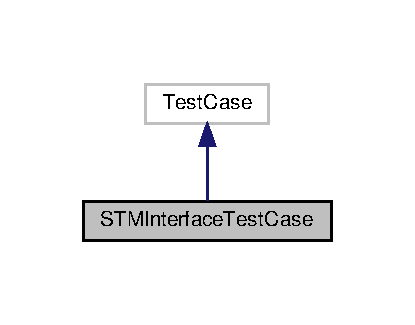
\includegraphics[width=199pt]{classstm__tools_1_1tests_1_1stmdevice__test_1_1STMInterfaceTestCase__inherit__graph}
\end{center}
\end{figure}


Collaboration diagram for S\+T\+M\+Interface\+Test\+Case\+:
\nopagebreak
\begin{figure}[H]
\begin{center}
\leavevmode
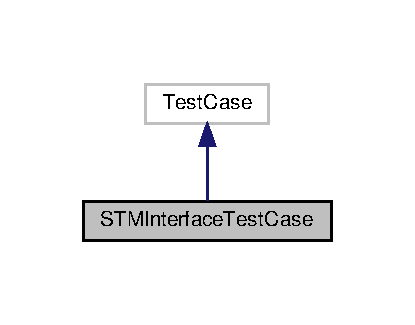
\includegraphics[width=199pt]{classstm__tools_1_1tests_1_1stmdevice__test_1_1STMInterfaceTestCase__coll__graph}
\end{center}
\end{figure}
\subsection*{Public Member Functions}
\begin{DoxyCompactItemize}
\item 
def \hyperlink{classstm__tools_1_1tests_1_1stmdevice__test_1_1STMInterfaceTestCase_a26b1b5aaa859d024cb7114cc1d4c1fd2}{set\+Up} (self)
\item 
def \hyperlink{classstm__tools_1_1tests_1_1stmdevice__test_1_1STMInterfaceTestCase_a56c54e463c817da67a20bb5e7b3b433a}{tear\+Down} (self)
\item 
def \hyperlink{classstm__tools_1_1tests_1_1stmdevice__test_1_1STMInterfaceTestCase_a3c64ad4ffc70313fb320cbff348ca340}{reset\+Device} (self)
\item 
def \hyperlink{classstm__tools_1_1tests_1_1stmdevice__test_1_1STMInterfaceTestCase_a408546ad5706980a509ac7d4226ba788}{test\+Get\+Device\+Information} (self)
\item 
def \hyperlink{classstm__tools_1_1tests_1_1stmdevice__test_1_1STMInterfaceTestCase_adda90c9c5669430e397f90131dc266b8}{test\+Get\+Device\+Bootloader\+Version} (self)
\item 
def \hyperlink{classstm__tools_1_1tests_1_1stmdevice__test_1_1STMInterfaceTestCase_a2df5f9e6a3f10a0160b330a5555b0f21}{test\+Get\+Device\+Bootloader\+Version\+Before\+Read} (self)
\item 
def \hyperlink{classstm__tools_1_1tests_1_1stmdevice__test_1_1STMInterfaceTestCase_a605c545bac14cf3b02c66ccbd9376603}{test\+Get\+Device\+Id\+Before\+Read} (self)
\item 
def \hyperlink{classstm__tools_1_1tests_1_1stmdevice__test_1_1STMInterfaceTestCase_a517f69dd76d9495fea814b05a467e25f}{test\+Write\+Data\+To\+Ram} (self)
\begin{DoxyCompactList}\small\item\em Test writing and reading to R\+AM \#\#\#. \end{DoxyCompactList}\item 
def \hyperlink{classstm__tools_1_1tests_1_1stmdevice__test_1_1STMInterfaceTestCase_a39b83e18c29c4fadb52969c6a26d9df2}{test\+Read\+Data\+From\+Ram} (self)
\item 
def \hyperlink{classstm__tools_1_1tests_1_1stmdevice__test_1_1STMInterfaceTestCase_a367136f856eff34bbd98d109c116b532}{test\+Write\+Data\+To\+Flash} (self)
\item 
def \hyperlink{classstm__tools_1_1tests_1_1stmdevice__test_1_1STMInterfaceTestCase_ad24b5e238a3322160c33e350ca7a4bd0}{test\+Read\+Data\+From\+Flash} (self)
\item 
def \hyperlink{classstm__tools_1_1tests_1_1stmdevice__test_1_1STMInterfaceTestCase_a62444780adc2068779a899c912837681}{test\+Read\+Option\+Bytes\+Data} (self)
\begin{DoxyCompactList}\small\item\em Test using the Flash and option bytes \#\#\#. \end{DoxyCompactList}\item 
def \hyperlink{classstm__tools_1_1tests_1_1stmdevice__test_1_1STMInterfaceTestCase_a19f0718574b25d07f4715ec0c9caad53}{test\+Write\+Option\+Bytes\+Data} (self)
\item 
def \hyperlink{classstm__tools_1_1tests_1_1stmdevice__test_1_1STMInterfaceTestCase_a18428729aed5aa4d5490942cada28264}{test\+Read\+Unprotect} (self)
\item 
def \hyperlink{classstm__tools_1_1tests_1_1stmdevice__test_1_1STMInterfaceTestCase_a709696307a75780772fda6f1c4544976}{test\+Read\+Protect} (self)
\item 
def \hyperlink{classstm__tools_1_1tests_1_1stmdevice__test_1_1STMInterfaceTestCase_aa3780a03aea7675aec22fb6dbf9af2e8}{test\+Long\+Write\+To\+Flash} (self)
\item 
def \hyperlink{classstm__tools_1_1tests_1_1stmdevice__test_1_1STMInterfaceTestCase_a69b3d280c74920034935b620de741818}{test\+Application\+Write\+To\+Flash} (self)
\end{DoxyCompactItemize}
\subsection*{Public Attributes}
\begin{DoxyCompactItemize}
\item 
\hyperlink{classstm__tools_1_1tests_1_1stmdevice__test_1_1STMInterfaceTestCase_ada855626ae0ce416b8edf41f44ab7bd5}{stm}
\end{DoxyCompactItemize}


\subsection{Member Function Documentation}
\mbox{\Hypertarget{classstm__tools_1_1tests_1_1stmdevice__test_1_1STMInterfaceTestCase_a3c64ad4ffc70313fb320cbff348ca340}\label{classstm__tools_1_1tests_1_1stmdevice__test_1_1STMInterfaceTestCase_a3c64ad4ffc70313fb320cbff348ca340}} 
\index{stm\+\_\+tools\+::tests\+::stmdevice\+\_\+test\+::\+S\+T\+M\+Interface\+Test\+Case@{stm\+\_\+tools\+::tests\+::stmdevice\+\_\+test\+::\+S\+T\+M\+Interface\+Test\+Case}!reset\+Device@{reset\+Device}}
\index{reset\+Device@{reset\+Device}!stm\+\_\+tools\+::tests\+::stmdevice\+\_\+test\+::\+S\+T\+M\+Interface\+Test\+Case@{stm\+\_\+tools\+::tests\+::stmdevice\+\_\+test\+::\+S\+T\+M\+Interface\+Test\+Case}}
\subsubsection{\texorpdfstring{reset\+Device()}{resetDevice()}}
{\footnotesize\ttfamily def reset\+Device (\begin{DoxyParamCaption}\item[{}]{self }\end{DoxyParamCaption})}

\mbox{\Hypertarget{classstm__tools_1_1tests_1_1stmdevice__test_1_1STMInterfaceTestCase_a26b1b5aaa859d024cb7114cc1d4c1fd2}\label{classstm__tools_1_1tests_1_1stmdevice__test_1_1STMInterfaceTestCase_a26b1b5aaa859d024cb7114cc1d4c1fd2}} 
\index{stm\+\_\+tools\+::tests\+::stmdevice\+\_\+test\+::\+S\+T\+M\+Interface\+Test\+Case@{stm\+\_\+tools\+::tests\+::stmdevice\+\_\+test\+::\+S\+T\+M\+Interface\+Test\+Case}!set\+Up@{set\+Up}}
\index{set\+Up@{set\+Up}!stm\+\_\+tools\+::tests\+::stmdevice\+\_\+test\+::\+S\+T\+M\+Interface\+Test\+Case@{stm\+\_\+tools\+::tests\+::stmdevice\+\_\+test\+::\+S\+T\+M\+Interface\+Test\+Case}}
\subsubsection{\texorpdfstring{set\+Up()}{setUp()}}
{\footnotesize\ttfamily def set\+Up (\begin{DoxyParamCaption}\item[{}]{self }\end{DoxyParamCaption})}

\mbox{\Hypertarget{classstm__tools_1_1tests_1_1stmdevice__test_1_1STMInterfaceTestCase_a56c54e463c817da67a20bb5e7b3b433a}\label{classstm__tools_1_1tests_1_1stmdevice__test_1_1STMInterfaceTestCase_a56c54e463c817da67a20bb5e7b3b433a}} 
\index{stm\+\_\+tools\+::tests\+::stmdevice\+\_\+test\+::\+S\+T\+M\+Interface\+Test\+Case@{stm\+\_\+tools\+::tests\+::stmdevice\+\_\+test\+::\+S\+T\+M\+Interface\+Test\+Case}!tear\+Down@{tear\+Down}}
\index{tear\+Down@{tear\+Down}!stm\+\_\+tools\+::tests\+::stmdevice\+\_\+test\+::\+S\+T\+M\+Interface\+Test\+Case@{stm\+\_\+tools\+::tests\+::stmdevice\+\_\+test\+::\+S\+T\+M\+Interface\+Test\+Case}}
\subsubsection{\texorpdfstring{tear\+Down()}{tearDown()}}
{\footnotesize\ttfamily def tear\+Down (\begin{DoxyParamCaption}\item[{}]{self }\end{DoxyParamCaption})}

\mbox{\Hypertarget{classstm__tools_1_1tests_1_1stmdevice__test_1_1STMInterfaceTestCase_a69b3d280c74920034935b620de741818}\label{classstm__tools_1_1tests_1_1stmdevice__test_1_1STMInterfaceTestCase_a69b3d280c74920034935b620de741818}} 
\index{stm\+\_\+tools\+::tests\+::stmdevice\+\_\+test\+::\+S\+T\+M\+Interface\+Test\+Case@{stm\+\_\+tools\+::tests\+::stmdevice\+\_\+test\+::\+S\+T\+M\+Interface\+Test\+Case}!test\+Application\+Write\+To\+Flash@{test\+Application\+Write\+To\+Flash}}
\index{test\+Application\+Write\+To\+Flash@{test\+Application\+Write\+To\+Flash}!stm\+\_\+tools\+::tests\+::stmdevice\+\_\+test\+::\+S\+T\+M\+Interface\+Test\+Case@{stm\+\_\+tools\+::tests\+::stmdevice\+\_\+test\+::\+S\+T\+M\+Interface\+Test\+Case}}
\subsubsection{\texorpdfstring{test\+Application\+Write\+To\+Flash()}{testApplicationWriteToFlash()}}
{\footnotesize\ttfamily def test\+Application\+Write\+To\+Flash (\begin{DoxyParamCaption}\item[{}]{self }\end{DoxyParamCaption})}

\mbox{\Hypertarget{classstm__tools_1_1tests_1_1stmdevice__test_1_1STMInterfaceTestCase_adda90c9c5669430e397f90131dc266b8}\label{classstm__tools_1_1tests_1_1stmdevice__test_1_1STMInterfaceTestCase_adda90c9c5669430e397f90131dc266b8}} 
\index{stm\+\_\+tools\+::tests\+::stmdevice\+\_\+test\+::\+S\+T\+M\+Interface\+Test\+Case@{stm\+\_\+tools\+::tests\+::stmdevice\+\_\+test\+::\+S\+T\+M\+Interface\+Test\+Case}!test\+Get\+Device\+Bootloader\+Version@{test\+Get\+Device\+Bootloader\+Version}}
\index{test\+Get\+Device\+Bootloader\+Version@{test\+Get\+Device\+Bootloader\+Version}!stm\+\_\+tools\+::tests\+::stmdevice\+\_\+test\+::\+S\+T\+M\+Interface\+Test\+Case@{stm\+\_\+tools\+::tests\+::stmdevice\+\_\+test\+::\+S\+T\+M\+Interface\+Test\+Case}}
\subsubsection{\texorpdfstring{test\+Get\+Device\+Bootloader\+Version()}{testGetDeviceBootloaderVersion()}}
{\footnotesize\ttfamily def test\+Get\+Device\+Bootloader\+Version (\begin{DoxyParamCaption}\item[{}]{self }\end{DoxyParamCaption})}

\begin{DoxyVerb}test we can get the expected device bootloader\end{DoxyVerb}
 \mbox{\Hypertarget{classstm__tools_1_1tests_1_1stmdevice__test_1_1STMInterfaceTestCase_a2df5f9e6a3f10a0160b330a5555b0f21}\label{classstm__tools_1_1tests_1_1stmdevice__test_1_1STMInterfaceTestCase_a2df5f9e6a3f10a0160b330a5555b0f21}} 
\index{stm\+\_\+tools\+::tests\+::stmdevice\+\_\+test\+::\+S\+T\+M\+Interface\+Test\+Case@{stm\+\_\+tools\+::tests\+::stmdevice\+\_\+test\+::\+S\+T\+M\+Interface\+Test\+Case}!test\+Get\+Device\+Bootloader\+Version\+Before\+Read@{test\+Get\+Device\+Bootloader\+Version\+Before\+Read}}
\index{test\+Get\+Device\+Bootloader\+Version\+Before\+Read@{test\+Get\+Device\+Bootloader\+Version\+Before\+Read}!stm\+\_\+tools\+::tests\+::stmdevice\+\_\+test\+::\+S\+T\+M\+Interface\+Test\+Case@{stm\+\_\+tools\+::tests\+::stmdevice\+\_\+test\+::\+S\+T\+M\+Interface\+Test\+Case}}
\subsubsection{\texorpdfstring{test\+Get\+Device\+Bootloader\+Version\+Before\+Read()}{testGetDeviceBootloaderVersionBeforeRead()}}
{\footnotesize\ttfamily def test\+Get\+Device\+Bootloader\+Version\+Before\+Read (\begin{DoxyParamCaption}\item[{}]{self }\end{DoxyParamCaption})}

\begin{DoxyVerb}test that getting bootloader version before read raises exception\end{DoxyVerb}
 \mbox{\Hypertarget{classstm__tools_1_1tests_1_1stmdevice__test_1_1STMInterfaceTestCase_a605c545bac14cf3b02c66ccbd9376603}\label{classstm__tools_1_1tests_1_1stmdevice__test_1_1STMInterfaceTestCase_a605c545bac14cf3b02c66ccbd9376603}} 
\index{stm\+\_\+tools\+::tests\+::stmdevice\+\_\+test\+::\+S\+T\+M\+Interface\+Test\+Case@{stm\+\_\+tools\+::tests\+::stmdevice\+\_\+test\+::\+S\+T\+M\+Interface\+Test\+Case}!test\+Get\+Device\+Id\+Before\+Read@{test\+Get\+Device\+Id\+Before\+Read}}
\index{test\+Get\+Device\+Id\+Before\+Read@{test\+Get\+Device\+Id\+Before\+Read}!stm\+\_\+tools\+::tests\+::stmdevice\+\_\+test\+::\+S\+T\+M\+Interface\+Test\+Case@{stm\+\_\+tools\+::tests\+::stmdevice\+\_\+test\+::\+S\+T\+M\+Interface\+Test\+Case}}
\subsubsection{\texorpdfstring{test\+Get\+Device\+Id\+Before\+Read()}{testGetDeviceIdBeforeRead()}}
{\footnotesize\ttfamily def test\+Get\+Device\+Id\+Before\+Read (\begin{DoxyParamCaption}\item[{}]{self }\end{DoxyParamCaption})}

\begin{DoxyVerb}test that getting device ID before read raises exception\end{DoxyVerb}
 \mbox{\Hypertarget{classstm__tools_1_1tests_1_1stmdevice__test_1_1STMInterfaceTestCase_a408546ad5706980a509ac7d4226ba788}\label{classstm__tools_1_1tests_1_1stmdevice__test_1_1STMInterfaceTestCase_a408546ad5706980a509ac7d4226ba788}} 
\index{stm\+\_\+tools\+::tests\+::stmdevice\+\_\+test\+::\+S\+T\+M\+Interface\+Test\+Case@{stm\+\_\+tools\+::tests\+::stmdevice\+\_\+test\+::\+S\+T\+M\+Interface\+Test\+Case}!test\+Get\+Device\+Information@{test\+Get\+Device\+Information}}
\index{test\+Get\+Device\+Information@{test\+Get\+Device\+Information}!stm\+\_\+tools\+::tests\+::stmdevice\+\_\+test\+::\+S\+T\+M\+Interface\+Test\+Case@{stm\+\_\+tools\+::tests\+::stmdevice\+\_\+test\+::\+S\+T\+M\+Interface\+Test\+Case}}
\subsubsection{\texorpdfstring{test\+Get\+Device\+Information()}{testGetDeviceInformation()}}
{\footnotesize\ttfamily def test\+Get\+Device\+Information (\begin{DoxyParamCaption}\item[{}]{self }\end{DoxyParamCaption})}

\begin{DoxyVerb}test we can read the device information\end{DoxyVerb}
 \mbox{\Hypertarget{classstm__tools_1_1tests_1_1stmdevice__test_1_1STMInterfaceTestCase_aa3780a03aea7675aec22fb6dbf9af2e8}\label{classstm__tools_1_1tests_1_1stmdevice__test_1_1STMInterfaceTestCase_aa3780a03aea7675aec22fb6dbf9af2e8}} 
\index{stm\+\_\+tools\+::tests\+::stmdevice\+\_\+test\+::\+S\+T\+M\+Interface\+Test\+Case@{stm\+\_\+tools\+::tests\+::stmdevice\+\_\+test\+::\+S\+T\+M\+Interface\+Test\+Case}!test\+Long\+Write\+To\+Flash@{test\+Long\+Write\+To\+Flash}}
\index{test\+Long\+Write\+To\+Flash@{test\+Long\+Write\+To\+Flash}!stm\+\_\+tools\+::tests\+::stmdevice\+\_\+test\+::\+S\+T\+M\+Interface\+Test\+Case@{stm\+\_\+tools\+::tests\+::stmdevice\+\_\+test\+::\+S\+T\+M\+Interface\+Test\+Case}}
\subsubsection{\texorpdfstring{test\+Long\+Write\+To\+Flash()}{testLongWriteToFlash()}}
{\footnotesize\ttfamily def test\+Long\+Write\+To\+Flash (\begin{DoxyParamCaption}\item[{}]{self }\end{DoxyParamCaption})}

\begin{DoxyVerb}test we can write a 516 len bytes to
flash memory, testing the multiple write
and remainder function
\end{DoxyVerb}
 \mbox{\Hypertarget{classstm__tools_1_1tests_1_1stmdevice__test_1_1STMInterfaceTestCase_ad24b5e238a3322160c33e350ca7a4bd0}\label{classstm__tools_1_1tests_1_1stmdevice__test_1_1STMInterfaceTestCase_ad24b5e238a3322160c33e350ca7a4bd0}} 
\index{stm\+\_\+tools\+::tests\+::stmdevice\+\_\+test\+::\+S\+T\+M\+Interface\+Test\+Case@{stm\+\_\+tools\+::tests\+::stmdevice\+\_\+test\+::\+S\+T\+M\+Interface\+Test\+Case}!test\+Read\+Data\+From\+Flash@{test\+Read\+Data\+From\+Flash}}
\index{test\+Read\+Data\+From\+Flash@{test\+Read\+Data\+From\+Flash}!stm\+\_\+tools\+::tests\+::stmdevice\+\_\+test\+::\+S\+T\+M\+Interface\+Test\+Case@{stm\+\_\+tools\+::tests\+::stmdevice\+\_\+test\+::\+S\+T\+M\+Interface\+Test\+Case}}
\subsubsection{\texorpdfstring{test\+Read\+Data\+From\+Flash()}{testReadDataFromFlash()}}
{\footnotesize\ttfamily def test\+Read\+Data\+From\+Flash (\begin{DoxyParamCaption}\item[{}]{self }\end{DoxyParamCaption})}

\begin{DoxyVerb}test we can read a byte from RAM\end{DoxyVerb}
 \mbox{\Hypertarget{classstm__tools_1_1tests_1_1stmdevice__test_1_1STMInterfaceTestCase_a39b83e18c29c4fadb52969c6a26d9df2}\label{classstm__tools_1_1tests_1_1stmdevice__test_1_1STMInterfaceTestCase_a39b83e18c29c4fadb52969c6a26d9df2}} 
\index{stm\+\_\+tools\+::tests\+::stmdevice\+\_\+test\+::\+S\+T\+M\+Interface\+Test\+Case@{stm\+\_\+tools\+::tests\+::stmdevice\+\_\+test\+::\+S\+T\+M\+Interface\+Test\+Case}!test\+Read\+Data\+From\+Ram@{test\+Read\+Data\+From\+Ram}}
\index{test\+Read\+Data\+From\+Ram@{test\+Read\+Data\+From\+Ram}!stm\+\_\+tools\+::tests\+::stmdevice\+\_\+test\+::\+S\+T\+M\+Interface\+Test\+Case@{stm\+\_\+tools\+::tests\+::stmdevice\+\_\+test\+::\+S\+T\+M\+Interface\+Test\+Case}}
\subsubsection{\texorpdfstring{test\+Read\+Data\+From\+Ram()}{testReadDataFromRam()}}
{\footnotesize\ttfamily def test\+Read\+Data\+From\+Ram (\begin{DoxyParamCaption}\item[{}]{self }\end{DoxyParamCaption})}

\begin{DoxyVerb}test we can read a byte from RAM\end{DoxyVerb}
 \mbox{\Hypertarget{classstm__tools_1_1tests_1_1stmdevice__test_1_1STMInterfaceTestCase_a62444780adc2068779a899c912837681}\label{classstm__tools_1_1tests_1_1stmdevice__test_1_1STMInterfaceTestCase_a62444780adc2068779a899c912837681}} 
\index{stm\+\_\+tools\+::tests\+::stmdevice\+\_\+test\+::\+S\+T\+M\+Interface\+Test\+Case@{stm\+\_\+tools\+::tests\+::stmdevice\+\_\+test\+::\+S\+T\+M\+Interface\+Test\+Case}!test\+Read\+Option\+Bytes\+Data@{test\+Read\+Option\+Bytes\+Data}}
\index{test\+Read\+Option\+Bytes\+Data@{test\+Read\+Option\+Bytes\+Data}!stm\+\_\+tools\+::tests\+::stmdevice\+\_\+test\+::\+S\+T\+M\+Interface\+Test\+Case@{stm\+\_\+tools\+::tests\+::stmdevice\+\_\+test\+::\+S\+T\+M\+Interface\+Test\+Case}}
\subsubsection{\texorpdfstring{test\+Read\+Option\+Bytes\+Data()}{testReadOptionBytesData()}}
{\footnotesize\ttfamily def test\+Read\+Option\+Bytes\+Data (\begin{DoxyParamCaption}\item[{}]{self }\end{DoxyParamCaption})}



Test using the Flash and option bytes \#\#\#. 

\mbox{\Hypertarget{classstm__tools_1_1tests_1_1stmdevice__test_1_1STMInterfaceTestCase_a709696307a75780772fda6f1c4544976}\label{classstm__tools_1_1tests_1_1stmdevice__test_1_1STMInterfaceTestCase_a709696307a75780772fda6f1c4544976}} 
\index{stm\+\_\+tools\+::tests\+::stmdevice\+\_\+test\+::\+S\+T\+M\+Interface\+Test\+Case@{stm\+\_\+tools\+::tests\+::stmdevice\+\_\+test\+::\+S\+T\+M\+Interface\+Test\+Case}!test\+Read\+Protect@{test\+Read\+Protect}}
\index{test\+Read\+Protect@{test\+Read\+Protect}!stm\+\_\+tools\+::tests\+::stmdevice\+\_\+test\+::\+S\+T\+M\+Interface\+Test\+Case@{stm\+\_\+tools\+::tests\+::stmdevice\+\_\+test\+::\+S\+T\+M\+Interface\+Test\+Case}}
\subsubsection{\texorpdfstring{test\+Read\+Protect()}{testReadProtect()}}
{\footnotesize\ttfamily def test\+Read\+Protect (\begin{DoxyParamCaption}\item[{}]{self }\end{DoxyParamCaption})}

\begin{DoxyVerb}assert we can successfully call readProtectFlashMemory
and assert that reads from flash fail
\end{DoxyVerb}
 \mbox{\Hypertarget{classstm__tools_1_1tests_1_1stmdevice__test_1_1STMInterfaceTestCase_a18428729aed5aa4d5490942cada28264}\label{classstm__tools_1_1tests_1_1stmdevice__test_1_1STMInterfaceTestCase_a18428729aed5aa4d5490942cada28264}} 
\index{stm\+\_\+tools\+::tests\+::stmdevice\+\_\+test\+::\+S\+T\+M\+Interface\+Test\+Case@{stm\+\_\+tools\+::tests\+::stmdevice\+\_\+test\+::\+S\+T\+M\+Interface\+Test\+Case}!test\+Read\+Unprotect@{test\+Read\+Unprotect}}
\index{test\+Read\+Unprotect@{test\+Read\+Unprotect}!stm\+\_\+tools\+::tests\+::stmdevice\+\_\+test\+::\+S\+T\+M\+Interface\+Test\+Case@{stm\+\_\+tools\+::tests\+::stmdevice\+\_\+test\+::\+S\+T\+M\+Interface\+Test\+Case}}
\subsubsection{\texorpdfstring{test\+Read\+Unprotect()}{testReadUnprotect()}}
{\footnotesize\ttfamily def test\+Read\+Unprotect (\begin{DoxyParamCaption}\item[{}]{self }\end{DoxyParamCaption})}

\mbox{\Hypertarget{classstm__tools_1_1tests_1_1stmdevice__test_1_1STMInterfaceTestCase_a367136f856eff34bbd98d109c116b532}\label{classstm__tools_1_1tests_1_1stmdevice__test_1_1STMInterfaceTestCase_a367136f856eff34bbd98d109c116b532}} 
\index{stm\+\_\+tools\+::tests\+::stmdevice\+\_\+test\+::\+S\+T\+M\+Interface\+Test\+Case@{stm\+\_\+tools\+::tests\+::stmdevice\+\_\+test\+::\+S\+T\+M\+Interface\+Test\+Case}!test\+Write\+Data\+To\+Flash@{test\+Write\+Data\+To\+Flash}}
\index{test\+Write\+Data\+To\+Flash@{test\+Write\+Data\+To\+Flash}!stm\+\_\+tools\+::tests\+::stmdevice\+\_\+test\+::\+S\+T\+M\+Interface\+Test\+Case@{stm\+\_\+tools\+::tests\+::stmdevice\+\_\+test\+::\+S\+T\+M\+Interface\+Test\+Case}}
\subsubsection{\texorpdfstring{test\+Write\+Data\+To\+Flash()}{testWriteDataToFlash()}}
{\footnotesize\ttfamily def test\+Write\+Data\+To\+Flash (\begin{DoxyParamCaption}\item[{}]{self }\end{DoxyParamCaption})}

\mbox{\Hypertarget{classstm__tools_1_1tests_1_1stmdevice__test_1_1STMInterfaceTestCase_a517f69dd76d9495fea814b05a467e25f}\label{classstm__tools_1_1tests_1_1stmdevice__test_1_1STMInterfaceTestCase_a517f69dd76d9495fea814b05a467e25f}} 
\index{stm\+\_\+tools\+::tests\+::stmdevice\+\_\+test\+::\+S\+T\+M\+Interface\+Test\+Case@{stm\+\_\+tools\+::tests\+::stmdevice\+\_\+test\+::\+S\+T\+M\+Interface\+Test\+Case}!test\+Write\+Data\+To\+Ram@{test\+Write\+Data\+To\+Ram}}
\index{test\+Write\+Data\+To\+Ram@{test\+Write\+Data\+To\+Ram}!stm\+\_\+tools\+::tests\+::stmdevice\+\_\+test\+::\+S\+T\+M\+Interface\+Test\+Case@{stm\+\_\+tools\+::tests\+::stmdevice\+\_\+test\+::\+S\+T\+M\+Interface\+Test\+Case}}
\subsubsection{\texorpdfstring{test\+Write\+Data\+To\+Ram()}{testWriteDataToRam()}}
{\footnotesize\ttfamily def test\+Write\+Data\+To\+Ram (\begin{DoxyParamCaption}\item[{}]{self }\end{DoxyParamCaption})}



Test writing and reading to R\+AM \#\#\#. 

\begin{DoxyVerb}test we can write a byte to RAM\end{DoxyVerb}
 \mbox{\Hypertarget{classstm__tools_1_1tests_1_1stmdevice__test_1_1STMInterfaceTestCase_a19f0718574b25d07f4715ec0c9caad53}\label{classstm__tools_1_1tests_1_1stmdevice__test_1_1STMInterfaceTestCase_a19f0718574b25d07f4715ec0c9caad53}} 
\index{stm\+\_\+tools\+::tests\+::stmdevice\+\_\+test\+::\+S\+T\+M\+Interface\+Test\+Case@{stm\+\_\+tools\+::tests\+::stmdevice\+\_\+test\+::\+S\+T\+M\+Interface\+Test\+Case}!test\+Write\+Option\+Bytes\+Data@{test\+Write\+Option\+Bytes\+Data}}
\index{test\+Write\+Option\+Bytes\+Data@{test\+Write\+Option\+Bytes\+Data}!stm\+\_\+tools\+::tests\+::stmdevice\+\_\+test\+::\+S\+T\+M\+Interface\+Test\+Case@{stm\+\_\+tools\+::tests\+::stmdevice\+\_\+test\+::\+S\+T\+M\+Interface\+Test\+Case}}
\subsubsection{\texorpdfstring{test\+Write\+Option\+Bytes\+Data()}{testWriteOptionBytesData()}}
{\footnotesize\ttfamily def test\+Write\+Option\+Bytes\+Data (\begin{DoxyParamCaption}\item[{}]{self }\end{DoxyParamCaption})}

\begin{DoxyVerb}test we can write a valid config to the option bytes
we check the value of the data byte to ensure write success
\end{DoxyVerb}
 

\subsection{Member Data Documentation}
\mbox{\Hypertarget{classstm__tools_1_1tests_1_1stmdevice__test_1_1STMInterfaceTestCase_ada855626ae0ce416b8edf41f44ab7bd5}\label{classstm__tools_1_1tests_1_1stmdevice__test_1_1STMInterfaceTestCase_ada855626ae0ce416b8edf41f44ab7bd5}} 
\index{stm\+\_\+tools\+::tests\+::stmdevice\+\_\+test\+::\+S\+T\+M\+Interface\+Test\+Case@{stm\+\_\+tools\+::tests\+::stmdevice\+\_\+test\+::\+S\+T\+M\+Interface\+Test\+Case}!stm@{stm}}
\index{stm@{stm}!stm\+\_\+tools\+::tests\+::stmdevice\+\_\+test\+::\+S\+T\+M\+Interface\+Test\+Case@{stm\+\_\+tools\+::tests\+::stmdevice\+\_\+test\+::\+S\+T\+M\+Interface\+Test\+Case}}
\subsubsection{\texorpdfstring{stm}{stm}}
{\footnotesize\ttfamily stm}



The documentation for this class was generated from the following file\+:\begin{DoxyCompactItemize}
\item 
/home/rich/\+Development/\+Py\+Dev/\+S\+T\+M32\+Tools/\+S\+T\+M32\+F1\+\_\+\+Serial\+\_\+\+Flasher/stm\+\_\+tools/tests/\hyperlink{stmdevice__test_8py}{stmdevice\+\_\+test.\+py}\end{DoxyCompactItemize}

\hypertarget{classstm__tools_1_1serialflasher_1_1errors_1_1UnexpectedResponseError}{}\section{Unexpected\+Response\+Error Class Reference}
\label{classstm__tools_1_1serialflasher_1_1errors_1_1UnexpectedResponseError}\index{Unexpected\+Response\+Error@{Unexpected\+Response\+Error}}


Inheritance diagram for Unexpected\+Response\+Error\+:
\nopagebreak
\begin{figure}[H]
\begin{center}
\leavevmode
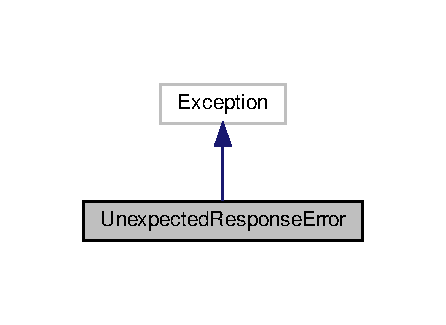
\includegraphics[width=214pt]{classstm__tools_1_1serialflasher_1_1errors_1_1UnexpectedResponseError__inherit__graph}
\end{center}
\end{figure}


Collaboration diagram for Unexpected\+Response\+Error\+:
\nopagebreak
\begin{figure}[H]
\begin{center}
\leavevmode
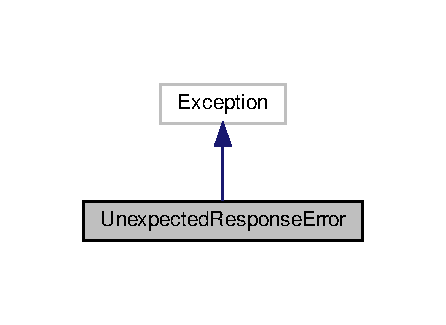
\includegraphics[width=214pt]{classstm__tools_1_1serialflasher_1_1errors_1_1UnexpectedResponseError__coll__graph}
\end{center}
\end{figure}


\subsection{Detailed Description}
\begin{DoxyVerb}An unexpected response was received\end{DoxyVerb}
 

The documentation for this class was generated from the following file\+:\begin{DoxyCompactItemize}
\item 
/home/rich/\+Development/\+Py\+Dev/\+S\+T\+M32\+Tools/\+S\+T\+M32\+F1\+\_\+\+Serial\+\_\+\+Flasher/stm\+\_\+tools/serialflasher/\hyperlink{errors_8py}{errors.\+py}\end{DoxyCompactItemize}

\hypertarget{classstm__tools_1_1serialflasher_1_1errors_1_1UnpackInfoFailedError}{}\section{Unpack\+Info\+Failed\+Error Class Reference}
\label{classstm__tools_1_1serialflasher_1_1errors_1_1UnpackInfoFailedError}\index{Unpack\+Info\+Failed\+Error@{Unpack\+Info\+Failed\+Error}}


Inheritance diagram for Unpack\+Info\+Failed\+Error\+:
\nopagebreak
\begin{figure}[H]
\begin{center}
\leavevmode
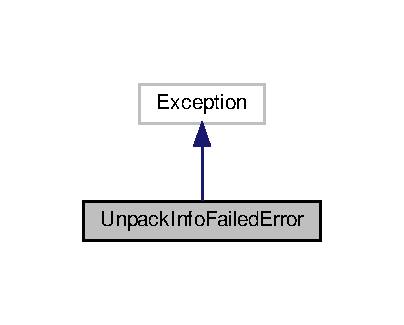
\includegraphics[width=194pt]{classstm__tools_1_1serialflasher_1_1errors_1_1UnpackInfoFailedError__inherit__graph}
\end{center}
\end{figure}


Collaboration diagram for Unpack\+Info\+Failed\+Error\+:
\nopagebreak
\begin{figure}[H]
\begin{center}
\leavevmode
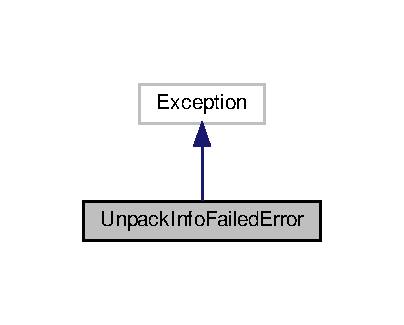
\includegraphics[width=194pt]{classstm__tools_1_1serialflasher_1_1errors_1_1UnpackInfoFailedError__coll__graph}
\end{center}
\end{figure}


\subsection{Detailed Description}
\begin{DoxyVerb}The info bytes were unable to be unpacked\end{DoxyVerb}
 

The documentation for this class was generated from the following file\+:\begin{DoxyCompactItemize}
\item 
/home/rich/\+Development/\+Py\+Dev/\+S\+T\+M32\+Tools/\+S\+T\+M32\+F1\+\_\+\+Serial\+\_\+\+Flasher/stm\+\_\+tools/serialflasher/\hyperlink{errors_8py}{errors.\+py}\end{DoxyCompactItemize}

\chapter{File Documentation}
\hypertarget{____init_____8py}{}\section{/home/rich/\+Development/\+Py\+Dev/\+S\+T\+M32\+Tools/\+S\+T\+M32\+F1\+\_\+\+Serial\+\_\+\+Flasher/stm\+\_\+tools/\+\_\+\+\_\+init\+\_\+\+\_\+.py File Reference}
\label{____init_____8py}\index{/home/rich/\+Development/\+Py\+Dev/\+S\+T\+M32\+Tools/\+S\+T\+M32\+F1\+\_\+\+Serial\+\_\+\+Flasher/stm\+\_\+tools/\+\_\+\+\_\+init\+\_\+\+\_\+.\+py@{/home/rich/\+Development/\+Py\+Dev/\+S\+T\+M32\+Tools/\+S\+T\+M32\+F1\+\_\+\+Serial\+\_\+\+Flasher/stm\+\_\+tools/\+\_\+\+\_\+init\+\_\+\+\_\+.\+py}}
\subsection*{Namespaces}
\begin{DoxyCompactItemize}
\item 
 \hyperlink{namespacestm__tools}{stm\+\_\+tools}
\end{DoxyCompactItemize}

\hypertarget{serialflasher_2____init_____8py}{}\section{/home/rich/\+Development/\+Py\+Dev/\+S\+T\+M32\+Tools/\+S\+T\+M32\+F1\+\_\+\+Serial\+\_\+\+Flasher/stm\+\_\+tools/serialflasher/\+\_\+\+\_\+init\+\_\+\+\_\+.py File Reference}
\label{serialflasher_2____init_____8py}\index{/home/rich/\+Development/\+Py\+Dev/\+S\+T\+M32\+Tools/\+S\+T\+M32\+F1\+\_\+\+Serial\+\_\+\+Flasher/stm\+\_\+tools/serialflasher/\+\_\+\+\_\+init\+\_\+\+\_\+.\+py@{/home/rich/\+Development/\+Py\+Dev/\+S\+T\+M32\+Tools/\+S\+T\+M32\+F1\+\_\+\+Serial\+\_\+\+Flasher/stm\+\_\+tools/serialflasher/\+\_\+\+\_\+init\+\_\+\+\_\+.\+py}}
\subsection*{Namespaces}
\begin{DoxyCompactItemize}
\item 
 \hyperlink{namespacestm__tools_1_1serialflasher}{stm\+\_\+tools.\+serialflasher}
\end{DoxyCompactItemize}

\hypertarget{tests_2____init_____8py}{}\section{/home/rich/\+Development/\+Py\+Dev/\+S\+T\+M32\+Tools/\+S\+T\+M32\+F1\+\_\+\+Serial\+\_\+\+Flasher/stm\+\_\+tools/tests/\+\_\+\+\_\+init\+\_\+\+\_\+.py File Reference}
\label{tests_2____init_____8py}\index{/home/rich/\+Development/\+Py\+Dev/\+S\+T\+M32\+Tools/\+S\+T\+M32\+F1\+\_\+\+Serial\+\_\+\+Flasher/stm\+\_\+tools/tests/\+\_\+\+\_\+init\+\_\+\+\_\+.\+py@{/home/rich/\+Development/\+Py\+Dev/\+S\+T\+M32\+Tools/\+S\+T\+M32\+F1\+\_\+\+Serial\+\_\+\+Flasher/stm\+\_\+tools/tests/\+\_\+\+\_\+init\+\_\+\+\_\+.\+py}}
\subsection*{Namespaces}
\begin{DoxyCompactItemize}
\item 
 \hyperlink{namespacestm__tools_1_1tests}{stm\+\_\+tools.\+tests}
\end{DoxyCompactItemize}

\hypertarget{constants_8py}{}\section{/home/rich/\+Development/\+Py\+Dev/\+S\+T\+M32\+Tools/\+S\+T\+M32\+F1\+\_\+\+Serial\+\_\+\+Flasher/stm\+\_\+tools/serialflasher/constants.py File Reference}
\label{constants_8py}\index{/home/rich/\+Development/\+Py\+Dev/\+S\+T\+M32\+Tools/\+S\+T\+M32\+F1\+\_\+\+Serial\+\_\+\+Flasher/stm\+\_\+tools/serialflasher/constants.\+py@{/home/rich/\+Development/\+Py\+Dev/\+S\+T\+M32\+Tools/\+S\+T\+M32\+F1\+\_\+\+Serial\+\_\+\+Flasher/stm\+\_\+tools/serialflasher/constants.\+py}}


contains constants used by the S\+TM bootloader  


\subsection*{Namespaces}
\begin{DoxyCompactItemize}
\item 
 \hyperlink{namespacestm__tools_1_1serialflasher_1_1constants}{stm\+\_\+tools.\+serialflasher.\+constants}
\end{DoxyCompactItemize}
\subsection*{Variables}
\begin{DoxyCompactItemize}
\item 
int \hyperlink{namespacestm__tools_1_1serialflasher_1_1constants_a8355cfda6a22b054771cec379e3687a9}{S\+T\+M\+\_\+\+R\+S\+P\+\_\+\+L\+E\+N\+\_\+\+B\+Y\+TE} = 1
\item 
int \hyperlink{namespacestm__tools_1_1serialflasher_1_1constants_a9fd4e692bfbfdcfce2aa0967c695b9cb}{S\+T\+M\+\_\+\+C\+M\+D\+\_\+\+H\+A\+N\+D\+S\+H\+A\+KE} = 0x7F
\item 
int \hyperlink{namespacestm__tools_1_1serialflasher_1_1constants_ac28ce0ad36785d1cd97a9341888c4e87}{S\+T\+M\+\_\+\+C\+M\+D\+\_\+\+A\+CK} = 0x79
\item 
int \hyperlink{namespacestm__tools_1_1serialflasher_1_1constants_aea0ea6655468a1b515f3ecc5c77fe132}{S\+T\+M\+\_\+\+C\+M\+D\+\_\+\+N\+A\+CK} = 0x1F
\item 
int \hyperlink{namespacestm__tools_1_1serialflasher_1_1constants_aec187f355bbd8d75889a8a888703b561}{S\+T\+M\+\_\+\+C\+M\+D\+\_\+\+G\+ET} = 0x00
\item 
int \hyperlink{namespacestm__tools_1_1serialflasher_1_1constants_a96496172df5836557db4edf3682fd14f}{S\+T\+M\+\_\+\+C\+M\+D\+\_\+\+V\+E\+R\+S\+I\+O\+N\+\_\+\+R\+E\+A\+D\+\_\+\+P\+R\+O\+T\+E\+CT} = 0x01
\item 
int \hyperlink{namespacestm__tools_1_1serialflasher_1_1constants_a9e6ba502dc8cf71e3ca09af43a27b50e}{S\+T\+M\+\_\+\+C\+M\+D\+\_\+\+G\+E\+T\+\_\+\+ID} = 0x02
\item 
int \hyperlink{namespacestm__tools_1_1serialflasher_1_1constants_a8a10a83309fd510330b5453140cb3516}{S\+T\+M\+\_\+\+C\+M\+D\+\_\+\+R\+E\+A\+D\+\_\+\+M\+EM} = 0x11
\item 
int \hyperlink{namespacestm__tools_1_1serialflasher_1_1constants_a98d4a1a9acc50ab78d8916ab797db74a}{S\+T\+M\+\_\+\+C\+M\+D\+\_\+\+GO} = 0x21
\item 
int \hyperlink{namespacestm__tools_1_1serialflasher_1_1constants_a88a947d173ce28afd93ef7937e3c17be}{S\+T\+M\+\_\+\+C\+M\+D\+\_\+\+W\+R\+I\+T\+E\+\_\+\+M\+EM} = 0x31
\item 
int \hyperlink{namespacestm__tools_1_1serialflasher_1_1constants_a9871a69524ee4c9871df968d4f1b6a37}{S\+T\+M\+\_\+\+C\+M\+D\+\_\+\+E\+R\+A\+S\+E\+\_\+\+M\+EM} = 0x43
\item 
int \hyperlink{namespacestm__tools_1_1serialflasher_1_1constants_ab3c1fb827d58301ab66a7d659220b6bd}{S\+T\+M\+\_\+\+C\+M\+D\+\_\+\+E\+X\+T\+\_\+\+E\+R\+A\+SE} = 0x44
\item 
int \hyperlink{namespacestm__tools_1_1serialflasher_1_1constants_a5d774c1771596f29cd18be93f349c5d3}{S\+T\+M\+\_\+\+C\+M\+D\+\_\+\+W\+R\+I\+T\+E\+\_\+\+P\+R\+O\+T\+E\+C\+T\+\_\+\+EN} = 0x63
\item 
int \hyperlink{namespacestm__tools_1_1serialflasher_1_1constants_acbb182b85efbf5850fe0435979ce7fd1}{S\+T\+M\+\_\+\+C\+M\+D\+\_\+\+W\+R\+I\+T\+E\+\_\+\+P\+R\+O\+T\+E\+C\+T\+\_\+\+D\+IS} = 0x73
\item 
int \hyperlink{namespacestm__tools_1_1serialflasher_1_1constants_a1b8e486151dc5e6f1e549b665d0682b6}{S\+T\+M\+\_\+\+C\+M\+D\+\_\+\+R\+E\+A\+D\+O\+U\+T\+\_\+\+P\+R\+O\+T\+E\+C\+T\+\_\+\+EN} = 0x82
\item 
int \hyperlink{namespacestm__tools_1_1serialflasher_1_1constants_a35e00bb803e9eaf44452c62752779e6f}{S\+T\+M\+\_\+\+C\+M\+D\+\_\+\+R\+E\+A\+D\+O\+U\+T\+\_\+\+P\+R\+O\+T\+E\+C\+T\+\_\+\+D\+IS} = 0x92
\item 
int \hyperlink{namespacestm__tools_1_1serialflasher_1_1constants_a7dd44899886a9e3035bb3b6746dd8203}{S\+T\+M\+\_\+\+G\+E\+T\+\_\+\+R\+E\+T\+U\+R\+N\+\_\+N} = 0x0B
\item 
int \hyperlink{namespacestm__tools_1_1serialflasher_1_1constants_a2115b42a2c641cb0bd3e49482c836530}{S\+T\+M\+\_\+\+R\+S\+P\+\_\+\+G\+E\+T\+\_\+\+L\+EN} = 12
\item 
int \hyperlink{namespacestm__tools_1_1serialflasher_1_1constants_a21ae2319bf1d542808d538fb56734263}{S\+T\+M\+\_\+\+G\+E\+T\+\_\+\+I\+D\+\_\+\+R\+S\+P\+\_\+\+L\+EN} = 2
\item 
int \hyperlink{namespacestm__tools_1_1serialflasher_1_1constants_ada4f39c4ccd1fbe20a1783d6b78024fe}{S\+T\+M\+\_\+\+V\+E\+R\+S\+\_\+\+R\+S\+P\+\_\+\+L\+EN} = 3
\item 
int \hyperlink{namespacestm__tools_1_1serialflasher_1_1constants_a2c47a48fe05305572ad6faa596f77346}{S\+T\+M\+\_\+\+B\+O\+O\+T\+L\+O\+A\+D\+E\+R\+\_\+\+M\+A\+X\+\_\+\+B\+A\+UD} = 115200
\item 
int \hyperlink{namespacestm__tools_1_1serialflasher_1_1constants_aaf62af7e54b0d4889b5df4707424ce3a}{S\+T\+M\+\_\+\+B\+O\+O\+T\+L\+O\+A\+D\+E\+R\+\_\+\+M\+I\+N\+\_\+\+B\+A\+UD} = 1200
\item 
int \hyperlink{namespacestm__tools_1_1serialflasher_1_1constants_a070aadb2eb435572cd9974a67a78b32c}{S\+T\+M\+\_\+\+F10\+X\+\_\+\+O\+P\+T\+B\+Y\+T\+E\+S\+\_\+\+A\+D\+DR} = 0x1\+F\+F\+F\+F800
\end{DoxyCompactItemize}


\subsection{Detailed Description}
contains constants used by the S\+TM bootloader 


\hypertarget{devices_8py}{}\section{/home/rich/\+Development/\+Py\+Dev/\+S\+T\+M32\+Tools/\+S\+T\+M32\+F1\+\_\+\+Serial\+\_\+\+Flasher/stm\+\_\+tools/serialflasher/devices.py File Reference}
\label{devices_8py}\index{/home/rich/\+Development/\+Py\+Dev/\+S\+T\+M32\+Tools/\+S\+T\+M32\+F1\+\_\+\+Serial\+\_\+\+Flasher/stm\+\_\+tools/serialflasher/devices.\+py@{/home/rich/\+Development/\+Py\+Dev/\+S\+T\+M32\+Tools/\+S\+T\+M32\+F1\+\_\+\+Serial\+\_\+\+Flasher/stm\+\_\+tools/serialflasher/devices.\+py}}
\subsection*{Classes}
\begin{DoxyCompactItemize}
\item 
class \hyperlink{classstm__tools_1_1serialflasher_1_1devices_1_1Region}{Region}
\item 
class \hyperlink{classstm__tools_1_1serialflasher_1_1devices_1_1DeviceDensity}{Device\+Density}
\item 
class \hyperlink{classstm__tools_1_1serialflasher_1_1devices_1_1OptionBytes}{Option\+Bytes}
\item 
class \hyperlink{classstm__tools_1_1serialflasher_1_1devices_1_1DeviceType}{Device\+Type}
\end{DoxyCompactItemize}
\subsection*{Namespaces}
\begin{DoxyCompactItemize}
\item 
 \hyperlink{namespacestm__tools_1_1serialflasher_1_1devices}{stm\+\_\+tools.\+serialflasher.\+devices}
\end{DoxyCompactItemize}
\subsection*{Variables}
\begin{DoxyCompactItemize}
\item 
\hyperlink{namespacestm__tools_1_1serialflasher_1_1devices_a929ea6db15a8a354b2e498af7e7caf7e}{Flash\+Option\+Bytes}
\end{DoxyCompactItemize}

\hypertarget{errors_8py}{}\section{/home/rich/\+Development/\+Py\+Dev/\+S\+T\+M32\+Tools/\+S\+T\+M32\+F1\+\_\+\+Serial\+\_\+\+Flasher/stm\+\_\+tools/serialflasher/errors.py File Reference}
\label{errors_8py}\index{/home/rich/\+Development/\+Py\+Dev/\+S\+T\+M32\+Tools/\+S\+T\+M32\+F1\+\_\+\+Serial\+\_\+\+Flasher/stm\+\_\+tools/serialflasher/errors.\+py@{/home/rich/\+Development/\+Py\+Dev/\+S\+T\+M32\+Tools/\+S\+T\+M32\+F1\+\_\+\+Serial\+\_\+\+Flasher/stm\+\_\+tools/serialflasher/errors.\+py}}
\subsection*{Classes}
\begin{DoxyCompactItemize}
\item 
class \hyperlink{classstm__tools_1_1serialflasher_1_1errors_1_1InformationNotRetrieved}{Information\+Not\+Retrieved}
\item 
class \hyperlink{classstm__tools_1_1serialflasher_1_1errors_1_1InvalidAddressError}{Invalid\+Address\+Error}
\item 
class \hyperlink{classstm__tools_1_1serialflasher_1_1errors_1_1InvalidReadLengthError}{Invalid\+Read\+Length\+Error}
\item 
class \hyperlink{classstm__tools_1_1serialflasher_1_1errors_1_1InvalidWriteLengthError}{Invalid\+Write\+Length\+Error}
\item 
class \hyperlink{classstm__tools_1_1serialflasher_1_1errors_1_1InvalidResponseLengthError}{Invalid\+Response\+Length\+Error}
\item 
class \hyperlink{classstm__tools_1_1serialflasher_1_1errors_1_1AckNotReceivedError}{Ack\+Not\+Received\+Error}
\item 
class \hyperlink{classstm__tools_1_1serialflasher_1_1errors_1_1NoResponseError}{No\+Response\+Error}
\item 
class \hyperlink{classstm__tools_1_1serialflasher_1_1errors_1_1UnexpectedResponseError}{Unexpected\+Response\+Error}
\item 
class \hyperlink{classstm__tools_1_1serialflasher_1_1errors_1_1InvalidEraseLengthError}{Invalid\+Erase\+Length\+Error}
\item 
class \hyperlink{classstm__tools_1_1serialflasher_1_1errors_1_1DeviceNotConnectedError}{Device\+Not\+Connected\+Error}
\item 
class \hyperlink{classstm__tools_1_1serialflasher_1_1errors_1_1CommandFailedError}{Command\+Failed\+Error}
\item 
class \hyperlink{classstm__tools_1_1serialflasher_1_1errors_1_1UnpackInfoFailedError}{Unpack\+Info\+Failed\+Error}
\item 
class \hyperlink{classstm__tools_1_1serialflasher_1_1errors_1_1DeviceNotSupportedError}{Device\+Not\+Supported\+Error}
\end{DoxyCompactItemize}
\subsection*{Namespaces}
\begin{DoxyCompactItemize}
\item 
 \hyperlink{namespacestm__tools_1_1serialflasher_1_1errors}{stm\+\_\+tools.\+serialflasher.\+errors}
\end{DoxyCompactItemize}

\hypertarget{serialtool_8py}{}\section{/home/rich/\+Development/\+Py\+Dev/\+S\+T\+M32\+Tools/\+S\+T\+M32\+F1\+\_\+\+Serial\+\_\+\+Flasher/stm\+\_\+tools/serialflasher/serialtool.py File Reference}
\label{serialtool_8py}\index{/home/rich/\+Development/\+Py\+Dev/\+S\+T\+M32\+Tools/\+S\+T\+M32\+F1\+\_\+\+Serial\+\_\+\+Flasher/stm\+\_\+tools/serialflasher/serialtool.\+py@{/home/rich/\+Development/\+Py\+Dev/\+S\+T\+M32\+Tools/\+S\+T\+M32\+F1\+\_\+\+Serial\+\_\+\+Flasher/stm\+\_\+tools/serialflasher/serialtool.\+py}}


Description\+: Python module creates an object with methods for interacting with the S\+T\+M32 F1 line of microcontrollers via the Bootloader\textquotesingle{}s serial interface.  


\subsection*{Classes}
\begin{DoxyCompactItemize}
\item 
class \hyperlink{classstm__tools_1_1serialflasher_1_1serialtool_1_1SerialTool}{Serial\+Tool}
\end{DoxyCompactItemize}
\subsection*{Namespaces}
\begin{DoxyCompactItemize}
\item 
 \hyperlink{namespacestm__tools_1_1serialflasher_1_1serialtool}{stm\+\_\+tools.\+serialflasher.\+serialtool}
\end{DoxyCompactItemize}


\subsection{Detailed Description}
Description\+: Python module creates an object with methods for interacting with the S\+T\+M32 F1 line of microcontrollers via the Bootloader\textquotesingle{}s serial interface. 


\hypertarget{stmdevice_8py}{}\section{/home/rich/\+Development/\+Py\+Dev/\+S\+T\+M32\+Tools/\+S\+T\+M32\+F1\+\_\+\+Serial\+\_\+\+Flasher/stm\+\_\+tools/serialflasher/stmdevice.py File Reference}
\label{stmdevice_8py}\index{/home/rich/\+Development/\+Py\+Dev/\+S\+T\+M32\+Tools/\+S\+T\+M32\+F1\+\_\+\+Serial\+\_\+\+Flasher/stm\+\_\+tools/serialflasher/stmdevice.\+py@{/home/rich/\+Development/\+Py\+Dev/\+S\+T\+M32\+Tools/\+S\+T\+M32\+F1\+\_\+\+Serial\+\_\+\+Flasher/stm\+\_\+tools/serialflasher/stmdevice.\+py}}
\subsection*{Classes}
\begin{DoxyCompactItemize}
\item 
class \hyperlink{classstm__tools_1_1serialflasher_1_1stmdevice_1_1STMInterface}{S\+T\+M\+Interface}
\end{DoxyCompactItemize}
\subsection*{Namespaces}
\begin{DoxyCompactItemize}
\item 
 \hyperlink{namespacestm__tools_1_1serialflasher_1_1stmdevice}{stm\+\_\+tools.\+serialflasher.\+stmdevice}
\end{DoxyCompactItemize}

\hypertarget{utilities_8py}{}\section{/home/rich/\+Development/\+Py\+Dev/\+S\+T\+M32\+Tools/\+S\+T\+M32\+F1\+\_\+\+Serial\+\_\+\+Flasher/stm\+\_\+tools/serialflasher/utilities.py File Reference}
\label{utilities_8py}\index{/home/rich/\+Development/\+Py\+Dev/\+S\+T\+M32\+Tools/\+S\+T\+M32\+F1\+\_\+\+Serial\+\_\+\+Flasher/stm\+\_\+tools/serialflasher/utilities.\+py@{/home/rich/\+Development/\+Py\+Dev/\+S\+T\+M32\+Tools/\+S\+T\+M32\+F1\+\_\+\+Serial\+\_\+\+Flasher/stm\+\_\+tools/serialflasher/utilities.\+py}}
\subsection*{Namespaces}
\begin{DoxyCompactItemize}
\item 
 \hyperlink{namespacestm__tools_1_1serialflasher_1_1utilities}{stm\+\_\+tools.\+serialflasher.\+utilities}
\end{DoxyCompactItemize}
\subsection*{Functions}
\begin{DoxyCompactItemize}
\item 
def \hyperlink{namespacestm__tools_1_1serialflasher_1_1utilities_a6b7d44fd38da6115bfc6e3eb77e6a69c}{unpack16\+Bit\+Int}
\item 
def \hyperlink{namespacestm__tools_1_1serialflasher_1_1utilities_a23faa11a3dac6cfd91613830f4bd8916}{get\+Byte\+Complement} (byte)
\item 
def \hyperlink{namespacestm__tools_1_1serialflasher_1_1utilities_aab173d5ef25c8fa59fbff1618da732ab}{clear\+Bit} (byte, bit)
\item 
def \hyperlink{namespacestm__tools_1_1serialflasher_1_1utilities_a6372484104fa9ee813d5f48004e551a4}{set\+Bit} (byte, bit)
\end{DoxyCompactItemize}

\hypertarget{devicetype__test_8py}{}\section{/home/rich/\+Development/\+Py\+Dev/\+S\+T\+M32\+Tools/\+S\+T\+M32\+F1\+\_\+\+Serial\+\_\+\+Flasher/stm\+\_\+tools/tests/devicetype\+\_\+test.py File Reference}
\label{devicetype__test_8py}\index{/home/rich/\+Development/\+Py\+Dev/\+S\+T\+M32\+Tools/\+S\+T\+M32\+F1\+\_\+\+Serial\+\_\+\+Flasher/stm\+\_\+tools/tests/devicetype\+\_\+test.\+py@{/home/rich/\+Development/\+Py\+Dev/\+S\+T\+M32\+Tools/\+S\+T\+M32\+F1\+\_\+\+Serial\+\_\+\+Flasher/stm\+\_\+tools/tests/devicetype\+\_\+test.\+py}}
\subsection*{Classes}
\begin{DoxyCompactItemize}
\item 
class \hyperlink{classstm__tools_1_1tests_1_1devicetype__test_1_1DeviceTypeTestCase}{Device\+Type\+Test\+Case}
\end{DoxyCompactItemize}
\subsection*{Namespaces}
\begin{DoxyCompactItemize}
\item 
 \hyperlink{namespacestm__tools_1_1tests_1_1devicetype__test}{stm\+\_\+tools.\+tests.\+devicetype\+\_\+test}
\end{DoxyCompactItemize}
\subsection*{Variables}
\begin{DoxyCompactItemize}
\item 
\hyperlink{namespacestm__tools_1_1tests_1_1devicetype__test_a673b122c6c4c7ffc0843953ef69a6990}{D\+E\+V\+\_\+\+T\+E\+S\+T\+\_\+\+X\+L\+\_\+\+D\+E\+V\+I\+C\+E\+\_\+\+ID}
\item 
\hyperlink{namespacestm__tools_1_1tests_1_1devicetype__test_ada001cf59610dae773467257abade9b1}{D\+E\+V\+\_\+\+T\+E\+S\+T\+\_\+\+V\+A\+L\+I\+D\+\_\+\+D\+E\+V\+I\+C\+E\+\_\+\+ID}
\item 
\hyperlink{namespacestm__tools_1_1tests_1_1devicetype__test_abeb943b6d91f9df1bffc0b026c26bce4}{D\+E\+V\+\_\+\+T\+E\+S\+T\+\_\+\+I\+N\+V\+A\+L\+I\+D\+\_\+\+D\+E\+V\+I\+C\+E\+\_\+\+ID}
\item 
\hyperlink{namespacestm__tools_1_1tests_1_1devicetype__test_ac6adf6af40a6afd2e7af8902b24c3cc1}{D\+E\+V\+\_\+\+T\+E\+S\+T\+\_\+\+V\+A\+L\+I\+D\+\_\+\+B\+O\+O\+T\+L\+O\+A\+D\+E\+R\+\_\+\+ID}
\item 
\hyperlink{namespacestm__tools_1_1tests_1_1devicetype__test_a81339cebc02ac225ee94cf1b272d37e2}{D\+E\+V\+\_\+\+T\+E\+S\+T\+\_\+\+V\+A\+L\+I\+D\+\_\+\+D\+E\+V\+I\+C\+E\+\_\+\+P\+A\+G\+E\+\_\+\+S\+I\+ZE}
\item 
\hyperlink{namespacestm__tools_1_1tests_1_1devicetype__test_a64b07338c65bc4dcded6e6e2570e4827}{D\+E\+V\+I\+C\+E\+T\+Y\+P\+E\+\_\+\+T\+E\+S\+T\+\_\+\+E\+X\+A\+M\+P\+L\+E\+\_\+\+O\+P\+T\+B\+Y\+T\+ES}
\end{DoxyCompactItemize}

\hypertarget{optionbytes__test_8py}{}\section{/home/rich/\+Development/\+Py\+Dev/\+S\+T\+M32\+Tools/\+S\+T\+M32\+F1\+\_\+\+Serial\+\_\+\+Flasher/stm\+\_\+tools/tests/optionbytes\+\_\+test.py File Reference}
\label{optionbytes__test_8py}\index{/home/rich/\+Development/\+Py\+Dev/\+S\+T\+M32\+Tools/\+S\+T\+M32\+F1\+\_\+\+Serial\+\_\+\+Flasher/stm\+\_\+tools/tests/optionbytes\+\_\+test.\+py@{/home/rich/\+Development/\+Py\+Dev/\+S\+T\+M32\+Tools/\+S\+T\+M32\+F1\+\_\+\+Serial\+\_\+\+Flasher/stm\+\_\+tools/tests/optionbytes\+\_\+test.\+py}}
\subsection*{Classes}
\begin{DoxyCompactItemize}
\item 
class \hyperlink{classstm__tools_1_1tests_1_1optionbytes__test_1_1OptioByteTestCase}{Optio\+Byte\+Test\+Case}
\end{DoxyCompactItemize}
\subsection*{Namespaces}
\begin{DoxyCompactItemize}
\item 
 \hyperlink{namespacestm__tools_1_1tests_1_1optionbytes__test}{stm\+\_\+tools.\+tests.\+optionbytes\+\_\+test}
\end{DoxyCompactItemize}
\subsection*{Variables}
\begin{DoxyCompactItemize}
\item 
\hyperlink{namespacestm__tools_1_1tests_1_1optionbytes__test_ab4140eb8a7fc0c05852f13a5aa961cf4}{O\+P\+T\+B\+Y\+T\+E\+\_\+\+T\+E\+S\+T\+\_\+\+V\+A\+L\+I\+D\+\_\+\+O\+P\+T\+I\+O\+N\+\_\+\+B\+Y\+T\+ES}
\end{DoxyCompactItemize}

\hypertarget{serialflasher__test_8py}{}\section{/home/rich/\+Development/\+Py\+Dev/\+S\+T\+M32\+Tools/\+S\+T\+M32\+F1\+\_\+\+Serial\+\_\+\+Flasher/stm\+\_\+tools/tests/serialflasher\+\_\+test.py File Reference}
\label{serialflasher__test_8py}\index{/home/rich/\+Development/\+Py\+Dev/\+S\+T\+M32\+Tools/\+S\+T\+M32\+F1\+\_\+\+Serial\+\_\+\+Flasher/stm\+\_\+tools/tests/serialflasher\+\_\+test.\+py@{/home/rich/\+Development/\+Py\+Dev/\+S\+T\+M32\+Tools/\+S\+T\+M32\+F1\+\_\+\+Serial\+\_\+\+Flasher/stm\+\_\+tools/tests/serialflasher\+\_\+test.\+py}}


unit tests for the Serial\+Flasher class First attempt at test-\/driven development Write a driver to interface with the S\+TM F1 series of chips Want to provide interface to\+:  


\subsection*{Classes}
\begin{DoxyCompactItemize}
\item 
class \hyperlink{classstm__tools_1_1tests_1_1serialflasher__test_1_1SerialFlasherTestCase}{Serial\+Flasher\+Test\+Case}
\end{DoxyCompactItemize}
\subsection*{Namespaces}
\begin{DoxyCompactItemize}
\item 
 \hyperlink{namespacestm__tools_1_1tests_1_1serialflasher__test}{stm\+\_\+tools.\+tests.\+serialflasher\+\_\+test}
\end{DoxyCompactItemize}
\subsection*{Variables}
\begin{DoxyCompactItemize}
\item 
\hyperlink{namespacestm__tools_1_1tests_1_1serialflasher__test_a76121998433d06c203d1657532f76250}{V\+A\+L\+I\+D\+\_\+\+P\+O\+RT}
\item 
\hyperlink{namespacestm__tools_1_1tests_1_1serialflasher__test_a1ebc242e7a86c50a6b683dc73d435fc0}{I\+N\+V\+A\+L\+I\+D\+\_\+\+P\+O\+RT}
\item 
\hyperlink{namespacestm__tools_1_1tests_1_1serialflasher__test_ad9f9c99c9f1d74f4a5d2ca206cacb192}{C\+M\+D\+\_\+\+H\+A\+N\+D\+S\+H\+A\+KE}
\item 
\hyperlink{namespacestm__tools_1_1tests_1_1serialflasher__test_afa84d84f05c3b4e9a82eed55bc91c729}{S\+T\+M\+\_\+\+A\+CK}
\item 
\hyperlink{namespacestm__tools_1_1tests_1_1serialflasher__test_a69ac6aa3b441f56a130f18e70d89529f}{D\+E\+V\+I\+C\+E\+\_\+\+S\+E\+R\+I\+A\+L\+\_\+\+P\+O\+RT}
\item 
\hyperlink{namespacestm__tools_1_1tests_1_1serialflasher__test_a18e6583da27755e0b79086411e0932a6}{D\+E\+V\+I\+C\+E\+\_\+\+S\+E\+R\+I\+A\+L\+\_\+\+B\+A\+UD}
\item 
\hyperlink{namespacestm__tools_1_1tests_1_1serialflasher__test_a59d8d0899dec790143b7694e3ba7869e}{D\+E\+V\+I\+C\+E\+\_\+\+S\+E\+R\+I\+A\+L\+\_\+\+W\+R\+T\+\_\+\+T\+I\+M\+E\+O\+U\+T\+\_\+S}
\item 
\hyperlink{namespacestm__tools_1_1tests_1_1serialflasher__test_a18b0d067d54847c27a1b1f67a69fd4af}{D\+E\+V\+I\+C\+E\+\_\+\+S\+E\+R\+I\+A\+L\+\_\+\+R\+D\+\_\+\+T\+I\+M\+E\+O\+U\+T\+\_\+S}
\item 
\hyperlink{namespacestm__tools_1_1tests_1_1serialflasher__test_af2963bac2a379526db940520efa35be7}{D\+E\+V\+I\+C\+E\+\_\+\+O\+P\+T\+I\+O\+N\+\_\+\+B\+Y\+T\+E\+S\+\_\+\+L\+EN}
\item 
\hyperlink{namespacestm__tools_1_1tests_1_1serialflasher__test_a57b992b4bb523a8c3196c0a250f5ed87}{D\+E\+V\+I\+C\+E\+\_\+\+S\+R\+A\+M\+\_\+\+S\+T\+A\+R\+T\+\_\+\+A\+D\+D\+R\+E\+SS}
\item 
\hyperlink{namespacestm__tools_1_1tests_1_1serialflasher__test_a4209a37586d60a3226b7bfc01faf8efa}{D\+E\+V\+I\+C\+E\+\_\+\+S\+R\+A\+M\+\_\+\+B\+O\+O\+T\+L\+O\+A\+D\+E\+R\+\_\+\+A\+D\+D\+R\+E\+SS}
\item 
\hyperlink{namespacestm__tools_1_1tests_1_1serialflasher__test_ae150c554225b93e1684f5845ea17e055}{D\+E\+V\+I\+C\+E\+\_\+\+A\+D\+D\+R\+\_\+\+O\+P\+T\+I\+O\+N\+B\+Y\+T\+ES}
\item 
\hyperlink{namespacestm__tools_1_1tests_1_1serialflasher__test_a65284c078af378de62bae59ea3f26d55}{D\+E\+V\+I\+C\+E\+\_\+\+I\+D\+\_\+\+E\+X\+P\+E\+C\+T\+E\+D\+\_\+\+B\+Y\+T\+ES}
\begin{DoxyCompactList}\small\item\em may have to refine this based on testing device! \end{DoxyCompactList}\item 
\hyperlink{namespacestm__tools_1_1tests_1_1serialflasher__test_a6dc3bf26591dbf1524ea88bea719f0df}{D\+E\+V\+I\+C\+E\+\_\+\+V\+A\+L\+I\+D\+\_\+\+B\+O\+O\+T\+L\+O\+A\+D\+E\+R\+\_\+\+V\+E\+R\+S\+I\+ON}
\item 
\hyperlink{namespacestm__tools_1_1tests_1_1serialflasher__test_a1cc886c6cbb9f9d5e24d9a50e7e6f4d1}{D\+E\+V\+I\+C\+E\+\_\+\+V\+A\+L\+I\+D\+\_\+\+C\+M\+DS}
\item 
\hyperlink{namespacestm__tools_1_1tests_1_1serialflasher__test_a01f375b415f66f35dfba69587829cd16}{S\+F\+\_\+\+T\+E\+S\+T\+\_\+\+R\+E\+A\+D\+\_\+\+A\+D\+D\+R\+\_\+\+O\+P\+T\+B\+Y\+T\+E\+S\+\_\+\+L\+EN}
\item 
\hyperlink{namespacestm__tools_1_1tests_1_1serialflasher__test_a500ed3fc7e37f3d6ef1aa3c1520e5a82}{S\+F\+\_\+\+T\+E\+S\+T\+\_\+\+D\+U\+M\+M\+Y\+\_\+\+D\+A\+TA}
\item 
\hyperlink{namespacestm__tools_1_1tests_1_1serialflasher__test_abb4df72148579487a6a4cca767c149fa}{S\+F\+\_\+\+T\+E\+S\+T\+\_\+\+F\+L\+A\+S\+H\+\_\+\+P\+A\+G\+E\+S\+\_\+\+E\+R\+A\+SE}
\item 
\hyperlink{namespacestm__tools_1_1tests_1_1serialflasher__test_a8393d2c2c4b44a58c07eed3b14b2f6ad}{S\+F\+\_\+\+T\+E\+S\+T\+\_\+\+W\+R\+I\+T\+E\+\_\+\+P\+R\+O\+T\+E\+C\+T\+\_\+\+S\+E\+C\+T\+O\+RS}
\item 
\hyperlink{namespacestm__tools_1_1tests_1_1serialflasher__test_ae1c42892dad519b503ef9a55a93aa16e}{S\+F\+\_\+\+T\+E\+S\+T\+\_\+\+S\+A\+M\+P\+L\+E\+\_\+\+B\+Y\+T\+E\+S\+\_\+\+N\+O\+\_\+\+C\+H\+E\+C\+K\+S\+UM}
\begin{DoxyCompactList}\small\item\em checksum8 X\+OR from \href{https://www.scadacore.com/tools/programming-calculators/online-checksum-calculator/}{\tt https\+://www.\+scadacore.\+com/tools/programming-\/calculators/online-\/checksum-\/calculator/} \end{DoxyCompactList}\item 
\hyperlink{namespacestm__tools_1_1tests_1_1serialflasher__test_afc86f38307068be6936b96ab60ddc7af}{S\+F\+\_\+\+T\+E\+S\+T\+\_\+\+S\+A\+M\+P\+L\+E\+\_\+\+B\+Y\+T\+E\+S\+\_\+\+W\+\_\+\+C\+H\+E\+C\+K\+S\+UM}
\end{DoxyCompactItemize}


\subsection{Detailed Description}
unit tests for the Serial\+Flasher class First attempt at test-\/driven development Write a driver to interface with the S\+TM F1 series of chips Want to provide interface to\+: 


\begin{DoxyItemize}
\item Connect with the device over serial U\+A\+RT
\item Read the device information
\item Read from a memory address
\item Write to a memory address
\item Lock/\+Unlock Flash sections
\item etc. 
\end{DoxyItemize}
\hypertarget{stmdevice__test_8py}{}\section{/home/rich/\+Development/\+Py\+Dev/\+S\+T\+M32\+Tools/\+S\+T\+M32\+F1\+\_\+\+Serial\+\_\+\+Flasher/stm\+\_\+tools/tests/stmdevice\+\_\+test.py File Reference}
\label{stmdevice__test_8py}\index{/home/rich/\+Development/\+Py\+Dev/\+S\+T\+M32\+Tools/\+S\+T\+M32\+F1\+\_\+\+Serial\+\_\+\+Flasher/stm\+\_\+tools/tests/stmdevice\+\_\+test.\+py@{/home/rich/\+Development/\+Py\+Dev/\+S\+T\+M32\+Tools/\+S\+T\+M32\+F1\+\_\+\+Serial\+\_\+\+Flasher/stm\+\_\+tools/tests/stmdevice\+\_\+test.\+py}}


tests for the \hyperlink{stmdevice_8py}{stmdevice.\+py} file  


\subsection*{Classes}
\begin{DoxyCompactItemize}
\item 
class \hyperlink{classstm__tools_1_1tests_1_1stmdevice__test_1_1STMInterfaceTestCase}{S\+T\+M\+Interface\+Test\+Case}
\end{DoxyCompactItemize}
\subsection*{Namespaces}
\begin{DoxyCompactItemize}
\item 
 \hyperlink{namespacestm__tools_1_1tests_1_1stmdevice__test}{stm\+\_\+tools.\+tests.\+stmdevice\+\_\+test}
\end{DoxyCompactItemize}
\subsection*{Functions}
\begin{DoxyCompactItemize}
\item 
def \hyperlink{namespacestm__tools_1_1tests_1_1stmdevice__test_a29847c5bc228bd343723ecd1954d48d3}{dump\+\_\+option\+\_\+bytes}
\end{DoxyCompactItemize}
\subsection*{Variables}
\begin{DoxyCompactItemize}
\item 
\hyperlink{namespacestm__tools_1_1tests_1_1stmdevice__test_a6dc3bf26591dbf1524ea88bea719f0df}{D\+E\+V\+I\+C\+E\+\_\+\+V\+A\+L\+I\+D\+\_\+\+B\+O\+O\+T\+L\+O\+A\+D\+E\+R\+\_\+\+V\+E\+R\+S\+I\+ON}
\item 
\hyperlink{namespacestm__tools_1_1tests_1_1stmdevice__test_a1cc886c6cbb9f9d5e24d9a50e7e6f4d1}{D\+E\+V\+I\+C\+E\+\_\+\+V\+A\+L\+I\+D\+\_\+\+C\+M\+DS}
\item 
\hyperlink{namespacestm__tools_1_1tests_1_1stmdevice__test_a69ac6aa3b441f56a130f18e70d89529f}{D\+E\+V\+I\+C\+E\+\_\+\+S\+E\+R\+I\+A\+L\+\_\+\+P\+O\+RT}
\item 
\hyperlink{namespacestm__tools_1_1tests_1_1stmdevice__test_a18e6583da27755e0b79086411e0932a6}{D\+E\+V\+I\+C\+E\+\_\+\+S\+E\+R\+I\+A\+L\+\_\+\+B\+A\+UD}
\item 
\hyperlink{namespacestm__tools_1_1tests_1_1stmdevice__test_a59d8d0899dec790143b7694e3ba7869e}{D\+E\+V\+I\+C\+E\+\_\+\+S\+E\+R\+I\+A\+L\+\_\+\+W\+R\+T\+\_\+\+T\+I\+M\+E\+O\+U\+T\+\_\+S}
\item 
\hyperlink{namespacestm__tools_1_1tests_1_1stmdevice__test_a18b0d067d54847c27a1b1f67a69fd4af}{D\+E\+V\+I\+C\+E\+\_\+\+S\+E\+R\+I\+A\+L\+\_\+\+R\+D\+\_\+\+T\+I\+M\+E\+O\+U\+T\+\_\+S}
\item 
\hyperlink{namespacestm__tools_1_1tests_1_1stmdevice__test_a2b12982688ba32b3f1a082db30996b9b}{D\+E\+V\+I\+C\+E\+\_\+\+T\+E\+S\+T\+\_\+\+R\+E\+A\+D\+\_\+\+I\+N\+V\+A\+L\+I\+D\+\_\+\+A\+D\+DR}
\item 
\hyperlink{namespacestm__tools_1_1tests_1_1stmdevice__test_ac638f3e012ffed2ccd9871fd5632270c}{S\+T\+M\+\_\+\+D\+E\+V\+I\+C\+E\+\_\+\+T\+E\+S\+T\+\_\+\+C\+H\+AR}
\item 
\hyperlink{namespacestm__tools_1_1tests_1_1stmdevice__test_a8c0b9134cc5952be4e65467c961cf5c8}{S\+T\+M\+\_\+\+T\+E\+S\+T\+\_\+\+V\+A\+L\+I\+D\+\_\+\+O\+P\+T\+B\+Y\+T\+E\+\_\+\+D\+A\+TA}
\item 
\hyperlink{namespacestm__tools_1_1tests_1_1stmdevice__test_a0642febd39ae1f1bdd3b615f59ffbc4d}{S\+T\+M\+\_\+\+T\+E\+S\+T\+\_\+\+B\+I\+N\+A\+R\+Y\+\_\+\+P\+A\+TH}
\item 
\hyperlink{namespacestm__tools_1_1tests_1_1stmdevice__test_a3e0eb2bdf03a525813ba2b19346e2b21}{S\+T\+M\+\_\+\+D\+E\+V\+I\+C\+E\+\_\+\+T\+E\+S\+T\+\_\+\+R\+A\+M\+\_\+\+A\+D\+DR}
\end{DoxyCompactItemize}


\subsection{Detailed Description}
tests for the \hyperlink{stmdevice_8py}{stmdevice.\+py} file 


%--- End generated contents ---

% Index
\backmatter
\newpage
\phantomsection
\clearemptydoublepage
\addcontentsline{toc}{chapter}{Index}
\printindex

\end{document}
